\documentclass{report}

%%%%%%%%%%%%%%%%%%%%%%%%%%%%%%%%%
% PACKAGE IMPORTS
%%%%%%%%%%%%%%%%%%%%%%%%%%%%%%%%%


\usepackage[tmargin=2cm,rmargin=1in,lmargin=1in,margin=0.85in,bmargin=2cm,footskip=.2in]{geometry}
\usepackage{amsmath,amsfonts,amsthm,amssymb,mathtools}
\usepackage[varbb]{newpxmath}
\usepackage{xfrac}
\usepackage[makeroom]{cancel}
\usepackage{mathtools}
\usepackage{bookmark}
\usepackage{enumitem}
\usepackage{hyperref,theoremref}
\hypersetup{
	pdftitle={Assignment},
	colorlinks=true, linkcolor=doc!90,
	bookmarksnumbered=true,
	bookmarksopen=true
}
\usepackage[most,many,breakable]{tcolorbox}
\usepackage{xcolor}
\usepackage{varwidth}
\usepackage{varwidth}
\usepackage{etoolbox}
%\usepackage{authblk}
\usepackage{nameref}
\usepackage{multicol,array}
\usepackage{tikz-cd}
\usepackage[ruled,vlined,linesnumbered]{algorithm2e}
\usepackage{comment} % enables the use of multi-line comments (\ifx \fi) 
\usepackage{import}
\usepackage{xifthen}
\usepackage{pdfpages}
\usepackage{transparent}
\usepackage[utf8]{inputenc}
\usepackage{fontawesome}


\newcommand\mycommfont[1]{\footnotesize\ttfamily\textcolor{blue}{#1}}
\SetCommentSty{mycommfont}
\newcommand{\incfig}[1]{%
    \def\svgwidth{\columnwidth}
    \import{./figures/}{#1.pdf_tex}
}

\usepackage{tikzsymbols}
\renewcommand{\qedsymbol}{\faWhatsapp}


%\usepackage{import}
%\usepackage{xifthen}
%\usepackage{pdfpages}
%\usepackage{transparent}


%%%%%%%%%%%%%%%%%%%%%%%%%%%%%%
% SELF MADE COLORS
%%%%%%%%%%%%%%%%%%%%%%%%%%%%%%



\definecolor{myg}{RGB}{56, 140, 70}
\definecolor{myb}{RGB}{45, 111, 177}
\definecolor{myr}{RGB}{199, 68, 64}
\definecolor{mytheorembg}{HTML}{F2F2F9}
\definecolor{mytheoremfr}{HTML}{00007B}
\definecolor{mylenmabg}{HTML}{FFFAF8}
\definecolor{mylenmafr}{HTML}{983b0f}
\definecolor{mypropbg}{HTML}{f2fbfc}
\definecolor{mypropfr}{HTML}{191971}
\definecolor{myexamplebg}{HTML}{F2FBF8}
\definecolor{myexamplefr}{HTML}{88D6D1}
\definecolor{myexampleti}{HTML}{2A7F7F}
\definecolor{mydefinitbg}{HTML}{E5E5FF}
\definecolor{mydefinitfr}{HTML}{3F3FA3}
\definecolor{notesgreen}{RGB}{0,162,0}
\definecolor{myp}{RGB}{197, 92, 212}
\definecolor{mygr}{HTML}{2C3338}
\definecolor{myred}{RGB}{127,0,0}
\definecolor{myyellow}{RGB}{169,121,69}
\definecolor{myexercisebg}{HTML}{F2FBF8}
\definecolor{myexercisefg}{HTML}{88D6D1}


%%%%%%%%%%%%%%%%%%%%%%%%%%%%
% TCOLORBOX SETUPS
%%%%%%%%%%%%%%%%%%%%%%%%%%%%

\setlength{\parindent}{1cm}
%================================
% THEOREM BOX
%================================

\tcbuselibrary{theorems,skins,hooks}
\newtcbtheorem[number within=section]{Theorem}{Theorem}
{%
	enhanced,
	breakable,
	colback = mytheorembg,
	frame hidden,
	boxrule = 0sp,
	borderline west = {2pt}{0pt}{mytheoremfr},
	sharp corners,
	detach title,
	before upper = \tcbtitle\par\smallskip,
	coltitle = mytheoremfr,
	fonttitle = \bfseries\sffamily,
	description font = \mdseries,
	separator sign none,
	segmentation style={solid, mytheoremfr},
}
{th}

\tcbuselibrary{theorems,skins,hooks}
\newtcbtheorem[number within=chapter]{theorem}{Theorem}
{%
	enhanced,
	breakable,
	colback = mytheorembg,
	frame hidden,
	boxrule = 0sp,
	borderline west = {2pt}{0pt}{mytheoremfr},
	sharp corners,
	detach title,
	before upper = \tcbtitle\par\smallskip,
	coltitle = mytheoremfr,
	fonttitle = \bfseries\sffamily,
	description font = \mdseries,
	separator sign none,
	segmentation style={solid, mytheoremfr},
}
{th}


\tcbuselibrary{theorems,skins,hooks}
\newtcolorbox{Theoremcon}
{%
	enhanced
	,breakable
	,colback = mytheorembg
	,frame hidden
	,boxrule = 0sp
	,borderline west = {2pt}{0pt}{mytheoremfr}
	,sharp corners
	,description font = \mdseries
	,separator sign none
}

%================================
% Corollery
%================================
\tcbuselibrary{theorems,skins,hooks}
\newtcbtheorem[number within=section]{Corollary}{Corollary}
{%
	enhanced
	,breakable
	,colback = myp!10
	,frame hidden
	,boxrule = 0sp
	,borderline west = {2pt}{0pt}{myp!85!black}
	,sharp corners
	,detach title
	,before upper = \tcbtitle\par\smallskip
	,coltitle = myp!85!black
	,fonttitle = \bfseries\sffamily
	,description font = \mdseries
	,separator sign none
	,segmentation style={solid, myp!85!black}
}
{th}
\tcbuselibrary{theorems,skins,hooks}
\newtcbtheorem[number within=chapter]{corollary}{Corollary}
{%
	enhanced
	,breakable
	,colback = myp!10
	,frame hidden
	,boxrule = 0sp
	,borderline west = {2pt}{0pt}{myp!85!black}
	,sharp corners
	,detach title
	,before upper = \tcbtitle\par\smallskip
	,coltitle = myp!85!black
	,fonttitle = \bfseries\sffamily
	,description font = \mdseries
	,separator sign none
	,segmentation style={solid, myp!85!black}
}
{th}


%================================
% LENMA
%================================

\tcbuselibrary{theorems,skins,hooks}
\newtcbtheorem[number within=section]{Lenma}{Lenma}
{%
	enhanced,
	breakable,
	colback = mylenmabg,
	frame hidden,
	boxrule = 0sp,
	borderline west = {2pt}{0pt}{mylenmafr},
	sharp corners,
	detach title,
	before upper = \tcbtitle\par\smallskip,
	coltitle = mylenmafr,
	fonttitle = \bfseries\sffamily,
	description font = \mdseries,
	separator sign none,
	segmentation style={solid, mylenmafr},
}
{th}

\tcbuselibrary{theorems,skins,hooks}
\newtcbtheorem[number within=chapter]{lenma}{Lenma}
{%
	enhanced,
	breakable,
	colback = mylenmabg,
	frame hidden,
	boxrule = 0sp,
	borderline west = {2pt}{0pt}{mylenmafr},
	sharp corners,
	detach title,
	before upper = \tcbtitle\par\smallskip,
	coltitle = mylenmafr,
	fonttitle = \bfseries\sffamily,
	description font = \mdseries,
	separator sign none,
	segmentation style={solid, mylenmafr},
}
{th}


%================================
% PROPOSITION
%================================

\tcbuselibrary{theorems,skins,hooks}
\newtcbtheorem[number within=section]{Prop}{Proposition}
{%
	enhanced,
	breakable,
	colback = mypropbg,
	frame hidden,
	boxrule = 0sp,
	borderline west = {2pt}{0pt}{mypropfr},
	sharp corners,
	detach title,
	before upper = \tcbtitle\par\smallskip,
	coltitle = mypropfr,
	fonttitle = \bfseries\sffamily,
	description font = \mdseries,
	separator sign none,
	segmentation style={solid, mypropfr},
}
{th}

\tcbuselibrary{theorems,skins,hooks}
\newtcbtheorem[number within=chapter]{prop}{Proposition}
{%
	enhanced,
	breakable,
	colback = mypropbg,
	frame hidden,
	boxrule = 0sp,
	borderline west = {2pt}{0pt}{mypropfr},
	sharp corners,
	detach title,
	before upper = \tcbtitle\par\smallskip,
	coltitle = mypropfr,
	fonttitle = \bfseries\sffamily,
	description font = \mdseries,
	separator sign none,
	segmentation style={solid, mypropfr},
}
{th}


%================================
% CLAIM
%================================

\tcbuselibrary{theorems,skins,hooks}
\newtcbtheorem[number within=section]{claim}{Claim}
{%
	enhanced
	,breakable
	,colback = myg!10
	,frame hidden
	,boxrule = 0sp
	,borderline west = {2pt}{0pt}{myg}
	,sharp corners
	,detach title
	,before upper = \tcbtitle\par\smallskip
	,coltitle = myg!85!black
	,fonttitle = \bfseries\sffamily
	,description font = \mdseries
	,separator sign none
	,segmentation style={solid, myg!85!black}
}
{th}



%================================
% Exercise
%================================

\tcbuselibrary{theorems,skins,hooks}
\newtcbtheorem[number within=section]{Exercise}{Exercise}
{%
	enhanced,
	breakable,
	colback = myexercisebg,
	frame hidden,
	boxrule = 0sp,
	borderline west = {2pt}{0pt}{myexercisefg},
	sharp corners,
	detach title,
	before upper = \tcbtitle\par\smallskip,
	coltitle = myexercisefg,
	fonttitle = \bfseries\sffamily,
	description font = \mdseries,
	separator sign none,
	segmentation style={solid, myexercisefg},
}
{th}

\tcbuselibrary{theorems,skins,hooks}
\newtcbtheorem[number within=chapter]{exercise}{Exercise}
{%
	enhanced,
	breakable,
	colback = myexercisebg,
	frame hidden,
	boxrule = 0sp,
	borderline west = {2pt}{0pt}{myexercisefg},
	sharp corners,
	detach title,
	before upper = \tcbtitle\par\smallskip,
	coltitle = myexercisefg,
	fonttitle = \bfseries\sffamily,
	description font = \mdseries,
	separator sign none,
	segmentation style={solid, myexercisefg},
}
{th}

%================================
% EXAMPLE BOX
%================================

\newtcbtheorem[number within=section]{Example}{Example}
{%
	colback = myexamplebg
	,breakable
	,colframe = myexamplefr
	,coltitle = myexampleti
	,boxrule = 1pt
	,sharp corners
	,detach title
	,before upper=\tcbtitle\par\smallskip
	,fonttitle = \bfseries
	,description font = \mdseries
	,separator sign none
	,description delimiters parenthesis
}
{ex}

\newtcbtheorem[number within=chapter]{example}{Example}
{%
	colback = myexamplebg
	,breakable
	,colframe = myexamplefr
	,coltitle = myexampleti
	,boxrule = 1pt
	,sharp corners
	,detach title
	,before upper=\tcbtitle\par\smallskip
	,fonttitle = \bfseries
	,description font = \mdseries
	,separator sign none
	,description delimiters parenthesis
}
{ex}

%================================
% DEFINITION BOX
%================================

\newtcbtheorem[number within=section]{Definition}{Definition}{enhanced,
	before skip=2mm,after skip=2mm, colback=red!5,colframe=red!80!black,boxrule=0.5mm,
	attach boxed title to top left={xshift=1cm,yshift*=1mm-\tcboxedtitleheight}, varwidth boxed title*=-3cm,
	boxed title style={frame code={
					\path[fill=tcbcolback]
					([yshift=-1mm,xshift=-1mm]frame.north west)
					arc[start angle=0,end angle=180,radius=1mm]
					([yshift=-1mm,xshift=1mm]frame.north east)
					arc[start angle=180,end angle=0,radius=1mm];
					\path[left color=tcbcolback!60!black,right color=tcbcolback!60!black,
						middle color=tcbcolback!80!black]
					([xshift=-2mm]frame.north west) -- ([xshift=2mm]frame.north east)
					[rounded corners=1mm]-- ([xshift=1mm,yshift=-1mm]frame.north east)
					-- (frame.south east) -- (frame.south west)
					-- ([xshift=-1mm,yshift=-1mm]frame.north west)
					[sharp corners]-- cycle;
				},interior engine=empty,
		},
	fonttitle=\bfseries,
	title={#2},#1}{def}
\newtcbtheorem[number within=chapter]{definition}{Definition}{enhanced,
	before skip=2mm,after skip=2mm, colback=red!5,colframe=red!80!black,boxrule=0.5mm,
	attach boxed title to top left={xshift=1cm,yshift*=1mm-\tcboxedtitleheight}, varwidth boxed title*=-3cm,
	boxed title style={frame code={
					\path[fill=tcbcolback]
					([yshift=-1mm,xshift=-1mm]frame.north west)
					arc[start angle=0,end angle=180,radius=1mm]
					([yshift=-1mm,xshift=1mm]frame.north east)
					arc[start angle=180,end angle=0,radius=1mm];
					\path[left color=tcbcolback!60!black,right color=tcbcolback!60!black,
						middle color=tcbcolback!80!black]
					([xshift=-2mm]frame.north west) -- ([xshift=2mm]frame.north east)
					[rounded corners=1mm]-- ([xshift=1mm,yshift=-1mm]frame.north east)
					-- (frame.south east) -- (frame.south west)
					-- ([xshift=-1mm,yshift=-1mm]frame.north west)
					[sharp corners]-- cycle;
				},interior engine=empty,
		},
	fonttitle=\bfseries,
	title={#2},#1}{def}



%================================
% Solution BOX
%================================

\makeatletter
\newtcbtheorem{question}{Question}{enhanced,
	breakable,
	colback=white,
	colframe=myb!80!black,
	attach boxed title to top left={yshift*=-\tcboxedtitleheight},
	fonttitle=\bfseries,
	title={#2},
	boxed title size=title,
	boxed title style={%
			sharp corners,
			rounded corners=northwest,
			colback=tcbcolframe,
			boxrule=0pt,
		},
	underlay boxed title={%
			\path[fill=tcbcolframe] (title.south west)--(title.south east)
			to[out=0, in=180] ([xshift=5mm]title.east)--
			(title.center-|frame.east)
			[rounded corners=\kvtcb@arc] |-
			(frame.north) -| cycle;
		},
	#1
}{def}
\makeatother

%================================
% SOLUTION BOX
%================================

\makeatletter
\newtcolorbox{solution}{enhanced,
	breakable,
	colback=white,
	colframe=myg!80!black,
	attach boxed title to top left={yshift*=-\tcboxedtitleheight},
	title=Solution,
	boxed title size=title,
	boxed title style={%
			sharp corners,
			rounded corners=northwest,
			colback=tcbcolframe,
			boxrule=0pt,
		},
	underlay boxed title={%
			\path[fill=tcbcolframe] (title.south west)--(title.south east)
			to[out=0, in=180] ([xshift=5mm]title.east)--
			(title.center-|frame.east)
			[rounded corners=\kvtcb@arc] |-
			(frame.north) -| cycle;
		},
}
\makeatother

%================================
% Question BOX
%================================

\makeatletter
\newtcbtheorem{qstion}{Question}{enhanced,
	breakable,
	colback=white,
	colframe=mygr,
	attach boxed title to top left={yshift*=-\tcboxedtitleheight},
	fonttitle=\bfseries,
	title={#2},
	boxed title size=title,
	boxed title style={%
			sharp corners,
			rounded corners=northwest,
			colback=tcbcolframe,
			boxrule=0pt,
		},
	underlay boxed title={%
			\path[fill=tcbcolframe] (title.south west)--(title.south east)
			to[out=0, in=180] ([xshift=5mm]title.east)--
			(title.center-|frame.east)
			[rounded corners=\kvtcb@arc] |-
			(frame.north) -| cycle;
		},
	#1
}{def}
\makeatother

\newtcbtheorem[number within=chapter]{wconc}{Wrong Concept}{
	breakable,
	enhanced,
	colback=white,
	colframe=myr,
	arc=0pt,
	outer arc=0pt,
	fonttitle=\bfseries\sffamily\large,
	colbacktitle=myr,
	attach boxed title to top left={},
	boxed title style={
			enhanced,
			skin=enhancedfirst jigsaw,
			arc=3pt,
			bottom=0pt,
			interior style={fill=myr}
		},
	#1
}{def}



%================================
% NOTE BOX
%================================

\usetikzlibrary{arrows,calc,shadows.blur}
\tcbuselibrary{skins}
\newtcolorbox{note}[1][]{%
	enhanced jigsaw,
	colback=gray!20!white,%
	colframe=gray!80!black,
	size=small,
	boxrule=1pt,
	title=\textbf{Note:},
	halign title=flush center,
	coltitle=black,
	breakable,
	drop shadow=black!50!white,
	attach boxed title to top left={xshift=1cm,yshift=-\tcboxedtitleheight/2,yshifttext=-\tcboxedtitleheight/2},
	minipage boxed title=1.5cm,
	boxed title style={%
			colback=white,
			size=fbox,
			boxrule=1pt,
			boxsep=2pt,
			underlay={%
					\coordinate (dotA) at ($(interior.west) + (-0.5pt,0)$);
					\coordinate (dotB) at ($(interior.east) + (0.5pt,0)$);
					\begin{scope}
						\clip (interior.north west) rectangle ([xshift=3ex]interior.east);
						\filldraw [white, blur shadow={shadow opacity=60, shadow yshift=-.75ex}, rounded corners=2pt] (interior.north west) rectangle (interior.south east);
					\end{scope}
					\begin{scope}[gray!80!black]
						\fill (dotA) circle (2pt);
						\fill (dotB) circle (2pt);
					\end{scope}
				},
		},
	#1,
}
%%%%%%%%%%%%%%%%%%%%%%%%%%%%
% CUSTOM AXIOMS BOX
%%%%%%%%%%%%%%%%%%%%%%%%%%%%
\newtcolorbox{AxiomsBox}{%
    enhanced,
    breakable,
    colback=mydefinitbg,
    colframe=mydefinitfr,
    boxrule=1pt,
    sharp corners,
    attach boxed title to top left={yshift*=-\tcboxedtitleheight},
    boxed title style={colback=mydefinitfr, coltitle=white, fonttitle=\bfseries\sffamily},
    title={Axioms of Probability},
}



%%%%%%%%%%%%%%%%%%%%%%%%%%%%%%
% SELF MADE COMMANDS
%%%%%%%%%%%%%%%%%%%%%%%%%%%%%%


\newcommand{\thm}[2]{\begin{Theorem}{#1}{}#2\end{Theorem}}
\newcommand{\cor}[2]{\begin{Corollary}{#1}{}#2\end{Corollary}}
\newcommand{\mlenma}[2]{\begin{Lenma}{#1}{}#2\end{Lenma}}
\newcommand{\mprop}[2]{\begin{Prop}{#1}{}#2\end{Prop}}
\newcommand{\clm}[3]{\begin{claim}{#1}{#2}#3\end{claim}}
\newcommand{\wc}[2]{\begin{wconc}{#1}{}\setlength{\parindent}{1cm}#2\end{wconc}}
\newcommand{\thmcon}[1]{\begin{Theoremcon}{#1}\end{Theoremcon}}
\newcommand{\ex}[2]{\begin{Example}{#1}{}#2\end{Example}}
\newcommand{\dfn}[2]{\begin{Definition}[colbacktitle=red!75!black]{#1}{}#2\end{Definition}}
\newcommand{\dfnc}[2]{\begin{definition}[colbacktitle=red!75!black]{#1}{}#2\end{definition}}
\newcommand{\qs}[2]{\begin{question}{#1}{}#2\end{question}}
\newcommand{\pf}[2]{\begin{myproof}[#1]#2\end{myproof}}
\newcommand{\nt}[1]{\begin{note}#1\end{note}}

\newcommand*\circled[1]{\tikz[baseline=(char.base)]{
		\node[shape=circle,draw,inner sep=1pt] (char) {#1};}}
\newcommand\getcurrentref[1]{%
	\ifnumequal{\value{#1}}{0}
	{??}
	{\the\value{#1}}%
}
\newcommand{\getCurrentSectionNumber}{\getcurrentref{section}}
\newenvironment{myproof}[1][\proofname]{%
	\proof[\bfseries #1: ]%
}{\endproof}

\newcommand{\mclm}[2]{\begin{myclaim}[#1]#2\end{myclaim}}
\newenvironment{myclaim}[1][\claimname]{\proof[\bfseries #1: ]}{}

\newcounter{mylabelcounter}

\makeatletter
\newcommand{\setword}[2]{%
	\phantomsection
	#1\def\@currentlabel{\unexpanded{#1}}\label{#2}%
}
\makeatother




\tikzset{
	symbol/.style={
			draw=none,
			every to/.append style={
					edge node={node [sloped, allow upside down, auto=false]{$#1$}}}
		}
}


% deliminators
\DeclarePairedDelimiter{\abs}{\lvert}{\rvert}
\DeclarePairedDelimiter{\norm}{\lVert}{\rVert}

\DeclarePairedDelimiter{\ceil}{\lceil}{\rceil}
\DeclarePairedDelimiter{\floor}{\lfloor}{\rfloor}
\DeclarePairedDelimiter{\round}{\lfloor}{\rceil}

\newsavebox\diffdbox
\newcommand{\slantedromand}{{\mathpalette\makesl{d}}}
\newcommand{\makesl}[2]{%
\begingroup
\sbox{\diffdbox}{$\mathsurround=0pt#1\mathrm{#2}$}%
\pdfsave
\pdfsetmatrix{1 0 0.2 1}%
\rlap{\usebox{\diffdbox}}%
\pdfrestore
\hskip\wd\diffdbox
\endgroup
}
\newcommand{\dd}[1][]{\ensuremath{\mathop{}\!\ifstrempty{#1}{%
\slantedromand\@ifnextchar^{\hspace{0.2ex}}{\hspace{0.1ex}}}%
{\slantedromand\hspace{0.2ex}^{#1}}}}
\ProvideDocumentCommand\dv{o m g}{%
  \ensuremath{%
    \IfValueTF{#3}{%
      \IfNoValueTF{#1}{%
        \frac{\dd #2}{\dd #3}%
      }{%
        \frac{\dd^{#1} #2}{\dd #3^{#1}}%
      }%
    }{%
      \IfNoValueTF{#1}{%
        \frac{\dd}{\dd #2}%
      }{%
        \frac{\dd^{#1}}{\dd #2^{#1}}%
      }%
    }%
  }%
}
\providecommand*{\pdv}[3][]{\frac{\partial^{#1}#2}{\partial#3^{#1}}}
%  - others
\DeclareMathOperator{\Lap}{\mathcal{L}}
\DeclareMathOperator{\Var}{Var} % varience
\DeclareMathOperator{\Cov}{Cov} % covarience
\DeclareMathOperator{\E}{E} % expected

% Since the amsthm package isn't loaded

% I prefer the slanted \leq
\let\oldleq\leq % save them in case they're every wanted
\let\oldgeq\geq
\renewcommand{\leq}{\leqslant}
\renewcommand{\geq}{\geqslant}

% % redefine matrix env to allow for alignment, use r as default
% \renewcommand*\env@matrix[1][r]{\hskip -\arraycolsep
%     \let\@ifnextchar\new@ifnextchar
%     \array{*\c@MaxMatrixCols #1}}


%\usepackage{framed}
%\usepackage{titletoc}
%\usepackage{etoolbox}
%\usepackage{lmodern}


%\patchcmd{\tableofcontents}{\contentsname}{\sffamily\contentsname}{}{}

%\renewenvironment{leftbar}
%{\def\FrameCommand{\hspace{6em}%
%		{\color{myyellow}\vrule width 2pt depth 6pt}\hspace{1em}}%
%	\MakeFramed{\parshape 1 0cm \dimexpr\textwidth-6em\relax\FrameRestore}\vskip2pt%
%}
%{\endMakeFramed}

%\titlecontents{chapter}
%[0em]{\vspace*{2\baselineskip}}
%{\parbox{4.5em}{%
%		\hfill\Huge\sffamily\bfseries\color{myred}\thecontentspage}%
%	\vspace*{-2.3\baselineskip}\leftbar\textsc{\small\chaptername~\thecontentslabel}\\\sffamily}
%{}{\endleftbar}
%\titlecontents{section}
%[8.4em]
%{\sffamily\contentslabel{3em}}{}{}
%{\hspace{0.5em}\nobreak\itshape\color{myred}\contentspage}
%\titlecontents{subsection}
%[8.4em]
%{\sffamily\contentslabel{3em}}{}{}  
%{\hspace{0.5em}\nobreak\itshape\color{myred}\contentspage}



%%%%%%%%%%%%%%%%%%%%%%%%%%%%%%%%%%%%%%%%%%%
% TABLE OF CONTENTS
%%%%%%%%%%%%%%%%%%%%%%%%%%%%%%%%%%%%%%%%%%%

\usepackage{tikz}
\definecolor{doc}{RGB}{0,60,110}
\usepackage{titletoc}
\contentsmargin{0cm}
\titlecontents{chapter}[3.7pc]
{\addvspace{30pt}%
	\begin{tikzpicture}[remember picture, overlay]%
		\draw[fill=doc!60,draw=doc!60] (-7,-.1) rectangle (-0.9,.5);%
		\pgftext[left,x=-3.5cm,y=0.2cm]{\color{white}\Large\sc\bfseries Chapter\ \thecontentslabel};%
	\end{tikzpicture}\color{doc!60}\large\sc\bfseries}%
{}
{}
{\;\titlerule\;\large\sc\bfseries Page \thecontentspage
	\begin{tikzpicture}[remember picture, overlay]
		\draw[fill=doc!60,draw=doc!60] (2pt,0) rectangle (4,0.1pt);
	\end{tikzpicture}}%
\titlecontents{section}[3.7pc]
{\addvspace{2pt}}
{\contentslabel[\thecontentslabel]{2pc}}
{}
{\hfill\small \thecontentspage}
[]
\titlecontents*{subsection}[3.7pc]
{\addvspace{-1pt}\small}
{}
{}
{\ --- \small\thecontentspage}
[ \textbullet\ ][]

\makeatletter
\renewcommand{\tableofcontents}{%
	\chapter*{%
	  \vspace*{-20\p@}%
	  \begin{tikzpicture}[remember picture, overlay]%
		  \pgftext[right,x=15cm,y=0.2cm]{\color{doc!60}\Huge\sc\bfseries \contentsname};%
		  \draw[fill=doc!60,draw=doc!60] (13,-.75) rectangle (20,1);%
		  \clip (13,-.75) rectangle (20,1);
		  \pgftext[right,x=15cm,y=0.2cm]{\color{white}\Huge\sc\bfseries \contentsname};%
	  \end{tikzpicture}}%
	\@starttoc{toc}}
\makeatother


% Comandi di Bastiality %
\newcommand{\innerproduct}[2]{\langle #1, #2 \rangle}
\newcommand{\generators}[1]{\langle #1 \rangle}
\newcommand{\powerset}[0]{\mathcal{P}}
\newcommand{\indip}{\perp \!\!\! \perp}

% Comandi di GioLaPalma %
\newcommand{\der}[0]{\implies^*}
\newcommand{\red}[1]{\textcolor{red}{#1}}
\newcommand{\esempio}[1]{\ex{}{#1}}
\newcommand{\teorema}[1]{\thm{}{#1}}
\newcommand{\dimostrazione}[1]{\pf{Dimostrazione}{#1}}
\setlength{\parindent}{0pt}
\newcommand{\osservazione}[1]{\nt{#1}}
\newcommand{\inside}[1]{
  \langle #1 \rangle
}
      

%From M275 "Topology" at SJSU
\newcommand{\id}{\mathrm{id}}
\newcommand{\taking}[1]{\xrightarrow{#1}}
\newcommand{\inv}{^{-1}}

%From M170 "Introduction to Graph Theory" at SJSU
\DeclareMathOperator{\diam}{diam}
\DeclareMathOperator{\ord}{ord}
\newcommand{\defeq}{\overset{\mathrm{def}}{=}}

%From the USAMO .tex files
\newcommand{\ts}{\textsuperscript}
\newcommand{\dg}{^\circ}
\newcommand{\ii}{\item}

% % From Math 55 and Math 145 at Harvard
% \newenvironment{subproof}[1][Proof]{%
% \begin{proof}[#1] \renewcommand{\qedsymbol}{$\blacksquare$}}%
% {\end{proof}}

\newcommand{\liff}{\leftrightarrow}
\newcommand{\lthen}{\rightarrow}
\newcommand{\opname}{\operatorname}
\newcommand{\surjto}{\twoheadrightarrow}
\newcommand{\injto}{\hookrightarrow}
\newcommand{\On}{\mathrm{On}} % ordinals
\DeclareMathOperator{\img}{im} % Image
\DeclareMathOperator{\Img}{Im} % Image
\DeclareMathOperator{\coker}{coker} % Cokernel
\DeclareMathOperator{\Coker}{Coker} % Cokernel
\DeclareMathOperator{\Ker}{Ker} % Kernel
\DeclareMathOperator{\rank}{rank}
\DeclareMathOperator{\Spec}{Spec} % spectrum
\DeclareMathOperator{\Tr}{Tr} % trace
\DeclareMathOperator{\pr}{pr} % projection
\DeclareMathOperator{\ext}{ext} % extension
\DeclareMathOperator{\pred}{pred} % predecessor
\DeclareMathOperator{\dom}{dom} % domain
\DeclareMathOperator{\ran}{ran} % range
\DeclareMathOperator{\Hom}{Hom} % homomorphism
\DeclareMathOperator{\Mor}{Mor} % morphisms
\DeclareMathOperator{\End}{End} % endomorphism

\newcommand{\eps}{\epsilon}
\newcommand{\veps}{\varepsilon}
\newcommand{\ol}{\overline}
\newcommand{\ul}{\underline}
\newcommand{\wt}{\widetilde}
\newcommand{\wh}{\widehat}
\newcommand{\vocab}[1]{\textbf{\color{blue} #1}}
\providecommand{\half}{\frac{1}{2}}
\newcommand{\dang}{\measuredangle} %% Directed angle
\newcommand{\ray}[1]{\overrightarrow{#1}}
\newcommand{\seg}[1]{\overline{#1}}
\newcommand{\arc}[1]{\wideparen{#1}}
\DeclareMathOperator{\cis}{cis}
\DeclareMathOperator*{\lcm}{lcm}
\DeclareMathOperator*{\argmin}{arg min}
\DeclareMathOperator*{\argmax}{arg max}
\newcommand{\cycsum}{\sum_{\mathrm{cyc}}}
\newcommand{\symsum}{\sum_{\mathrm{sym}}}
\newcommand{\cycprod}{\prod_{\mathrm{cyc}}}
\newcommand{\symprod}{\prod_{\mathrm{sym}}}
\newcommand{\Qed}{\begin{flushright}\qed\end{flushright}}
\newcommand{\parinn}{\setlength{\parindent}{1cm}}
\newcommand{\parinf}{\setlength{\parindent}{0cm}}
% \newcommand{\norm}{\|\cdot\|}
\newcommand{\inorm}{\norm_{\infty}}
\newcommand{\opensets}{\{V_{\alpha}\}_{\alpha\in I}}
\newcommand{\oset}{V_{\alpha}}
\newcommand{\opset}[1]{V_{\alpha_{#1}}}
\newcommand{\lub}{\text{lub}}
\newcommand{\del}[2]{\frac{\partial #1}{\partial #2}}
\newcommand{\Del}[3]{\frac{\partial^{#1} #2}{\partial^{#1} #3}}
\newcommand{\deld}[2]{\dfrac{\partial #1}{\partial #2}}
\newcommand{\Deld}[3]{\dfrac{\partial^{#1} #2}{\partial^{#1} #3}}
\newcommand{\lm}{\lambda}
\newcommand{\uin}{\mathbin{\rotatebox[origin=c]{90}{$\in$}}}
\newcommand{\usubset}{\mathbin{\rotatebox[origin=c]{90}{$\subset$}}}
\newcommand{\lt}{\left}
\newcommand{\rt}{\right}
\newcommand{\bs}[1]{\boldsymbol{#1}}
\newcommand{\exs}{\exists}
\newcommand{\st}{\strut}
\newcommand{\dps}[1]{\displaystyle{#1}}

\newcommand{\sol}{\setlength{\parindent}{0cm}\textbf{\textit{Solution:}}\setlength{\parindent}{1cm} }
\newcommand{\solve}[1]{\setlength{\parindent}{0cm}\textbf{\textit{Solution: }}\setlength{\parindent}{1cm}#1 \Qed}

% Things Lie
\newcommand{\kb}{\mathfrak b}
\newcommand{\kg}{\mathfrak g}
\newcommand{\kh}{\mathfrak h}
\newcommand{\kn}{\mathfrak n}
\newcommand{\ku}{\mathfrak u}
\newcommand{\kz}{\mathfrak z}
\DeclareMathOperator{\Ext}{Ext} % Ext functor
\DeclareMathOperator{\Tor}{Tor} % Tor functor
\newcommand{\gl}{\opname{\mathfrak{gl}}} % frak gl group
\renewcommand{\sl}{\opname{\mathfrak{sl}}} % frak sl group chktex 6

% More script letters etc.
\newcommand{\SA}{\mathcal A}
\newcommand{\SB}{\mathcal B}
\newcommand{\SC}{\mathcal C}
\newcommand{\SF}{\mathcal F}
\newcommand{\SG}{\mathcal G}
\newcommand{\SH}{\mathcal H}
\newcommand{\OO}{\mathcal O}

\newcommand{\SCA}{\mathscr A}
\newcommand{\SCB}{\mathscr B}
\newcommand{\SCC}{\mathscr C}
\newcommand{\SCD}{\mathscr D}
\newcommand{\SCE}{\mathscr E}
\newcommand{\SCF}{\mathscr F}
\newcommand{\SCG}{\mathscr G}
\newcommand{\SCH}{\mathscr H}

% Mathfrak primes
\newcommand{\km}{\mathfrak m}
\newcommand{\kp}{\mathfrak p}
\newcommand{\kq}{\mathfrak q}

% number sets
\newcommand{\RR}[1][]{\ensuremath{\ifstrempty{#1}{\mathbb{R}}{\mathbb{R}^{#1}}}}
\newcommand{\NN}[1][]{\ensuremath{\ifstrempty{#1}{\mathbb{N}}{\mathbb{N}^{#1}}}}
\newcommand{\ZZ}[1][]{\ensuremath{\ifstrempty{#1}{\mathbb{Z}}{\mathbb{Z}^{#1}}}}
\newcommand{\QQ}[1][]{\ensuremath{\ifstrempty{#1}{\mathbb{Q}}{\mathbb{Q}^{#1}}}}
\newcommand{\CC}[1][]{\ensuremath{\ifstrempty{#1}{\mathbb{C}}{\mathbb{C}^{#1}}}}
\newcommand{\PP}[1][]{\ensuremath{\ifstrempty{#1}{\mathbb{P}}{\mathbb{P}^{#1}}}}
\newcommand{\HH}[1][]{\ensuremath{\ifstrempty{#1}{\mathbb{H}}{\mathbb{H}^{#1}}}}
\newcommand{\FF}[1][]{\ensuremath{\ifstrempty{#1}{\mathbb{F}}{\mathbb{F}^{#1}}}}
% expected value
\newcommand{\EE}{\ensuremath{\mathbb{E}}}
\newcommand{\charin}{\text{ char }}
\DeclareMathOperator{\sign}{sign}
\DeclareMathOperator{\Aut}{Aut}
\DeclareMathOperator{\Inn}{Inn}
\DeclareMathOperator{\Syl}{Syl}
\DeclareMathOperator{\Gal}{Gal}
\DeclareMathOperator{\GL}{GL} % General linear group
\DeclareMathOperator{\SL}{SL} % Special linear group

%---------------------------------------
% BlackBoard Math Fonts :-
%---------------------------------------

%Captital Letters
\newcommand{\bbA}{\mathbb{A}}	\newcommand{\bbB}{\mathbb{B}}
\newcommand{\bbC}{\mathbb{C}}	\newcommand{\bbD}{\mathbb{D}}
\newcommand{\bbE}{\mathbb{E}}	\newcommand{\bbF}{\mathbb{F}}
\newcommand{\bbG}{\mathbb{G}}	\newcommand{\bbH}{\mathbb{H}}
\newcommand{\bbI}{\mathbb{I}}	\newcommand{\bbJ}{\mathbb{J}}
\newcommand{\bbK}{\mathbb{K}}	\newcommand{\bbL}{\mathbb{L}}
\newcommand{\bbM}{\mathbb{M}}	\newcommand{\bbN}{\mathbb{N}}
\newcommand{\bbO}{\mathbb{O}}	\newcommand{\bbP}{\mathbb{P}}
\newcommand{\bbQ}{\mathbb{Q}}	\newcommand{\bbR}{\mathbb{R}}
\newcommand{\bbS}{\mathbb{S}}	\newcommand{\bbT}{\mathbb{T}}
\newcommand{\bbU}{\mathbb{U}}	\newcommand{\bbV}{\mathbb{V}}
\newcommand{\bbW}{\mathbb{W}}	\newcommand{\bbX}{\mathbb{X}}
\newcommand{\bbY}{\mathbb{Y}}	\newcommand{\bbZ}{\mathbb{Z}}

%---------------------------------------
% MathCal Fonts :-
%---------------------------------------

%Captital Letters
\newcommand{\mcA}{\mathcal{A}}	\newcommand{\mcB}{\mathcal{B}}
\newcommand{\mcC}{\mathcal{C}}	\newcommand{\mcD}{\mathcal{D}}
\newcommand{\mcE}{\mathcal{E}}	\newcommand{\mcF}{\mathcal{F}}
\newcommand{\mcG}{\mathcal{G}}	\newcommand{\mcH}{\mathcal{H}}
\newcommand{\mcI}{\mathcal{I}}	\newcommand{\mcJ}{\mathcal{J}}
\newcommand{\mcK}{\mathcal{K}}	\newcommand{\mcL}{\mathcal{L}}
\newcommand{\mcM}{\mathcal{M}}	\newcommand{\mcN}{\mathcal{N}}
\newcommand{\mcO}{\mathcal{O}}	\newcommand{\mcP}{\mathcal{P}}
\newcommand{\mcQ}{\mathcal{Q}}	\newcommand{\mcR}{\mathcal{R}}
\newcommand{\mcS}{\mathcal{S}}	\newcommand{\mcT}{\mathcal{T}}
\newcommand{\mcU}{\mathcal{U}}	\newcommand{\mcV}{\mathcal{V}}
\newcommand{\mcW}{\mathcal{W}}	\newcommand{\mcX}{\mathcal{X}}
\newcommand{\mcY}{\mathcal{Y}}	\newcommand{\mcZ}{\mathcal{Z}}


%---------------------------------------
% Bold Math Fonts :-
%---------------------------------------

%Captital Letters
\newcommand{\bmA}{\boldsymbol{A}}	\newcommand{\bmB}{\boldsymbol{B}}
\newcommand{\bmC}{\boldsymbol{C}}	\newcommand{\bmD}{\boldsymbol{D}}
\newcommand{\bmE}{\boldsymbol{E}}	\newcommand{\bmF}{\boldsymbol{F}}
\newcommand{\bmG}{\boldsymbol{G}}	\newcommand{\bmH}{\boldsymbol{H}}
\newcommand{\bmI}{\boldsymbol{I}}	\newcommand{\bmJ}{\boldsymbol{J}}
\newcommand{\bmK}{\boldsymbol{K}}	\newcommand{\bmL}{\boldsymbol{L}}
\newcommand{\bmM}{\boldsymbol{M}}	\newcommand{\bmN}{\boldsymbol{N}}
\newcommand{\bmO}{\boldsymbol{O}}	\newcommand{\bmP}{\boldsymbol{P}}
\newcommand{\bmQ}{\boldsymbol{Q}}	\newcommand{\bmR}{\boldsymbol{R}}
\newcommand{\bmS}{\boldsymbol{S}}	\newcommand{\bmT}{\boldsymbol{T}}
\newcommand{\bmU}{\boldsymbol{U}}	\newcommand{\bmV}{\boldsymbol{V}}
\newcommand{\bmW}{\boldsymbol{W}}	\newcommand{\bmX}{\boldsymbol{X}}
\newcommand{\bmY}{\boldsymbol{Y}}	\newcommand{\bmZ}{\boldsymbol{Z}}
%Small Letters
\newcommand{\bma}{\boldsymbol{a}}	\newcommand{\bmb}{\boldsymbol{b}}
\newcommand{\bmc}{\boldsymbol{c}}	\newcommand{\bmd}{\boldsymbol{d}}
\newcommand{\bme}{\boldsymbol{e}}	\newcommand{\bmf}{\boldsymbol{f}}
\newcommand{\bmg}{\boldsymbol{g}}	\newcommand{\bmh}{\boldsymbol{h}}
\newcommand{\bmi}{\boldsymbol{i}}	\newcommand{\bmj}{\boldsymbol{j}}
\newcommand{\bmk}{\boldsymbol{k}}	\newcommand{\bml}{\boldsymbol{l}}
\newcommand{\bmm}{\boldsymbol{m}}	\newcommand{\bmn}{\boldsymbol{n}}
\newcommand{\bmo}{\boldsymbol{o}}	\newcommand{\bmp}{\boldsymbol{p}}
\newcommand{\bmq}{\boldsymbol{q}}	\newcommand{\bmr}{\boldsymbol{r}}
\newcommand{\bms}{\boldsymbol{s}}	\newcommand{\bmt}{\boldsymbol{t}}
\newcommand{\bmu}{\boldsymbol{u}}	\newcommand{\bmv}{\boldsymbol{v}}
\newcommand{\bmw}{\boldsymbol{w}}	\newcommand{\bmx}{\boldsymbol{x}}
\newcommand{\bmy}{\boldsymbol{y}}	\newcommand{\bmz}{\boldsymbol{z}}

%---------------------------------------
% Scr Math Fonts :-
%---------------------------------------

\newcommand{\sA}{{\mathscr{A}}}   \newcommand{\sB}{{\mathscr{B}}}
\newcommand{\sC}{{\mathscr{C}}}   \newcommand{\sD}{{\mathscr{D}}}
\newcommand{\sE}{{\mathscr{E}}}   \newcommand{\sF}{{\mathscr{F}}}
\newcommand{\sG}{{\mathscr{G}}}   \newcommand{\sH}{{\mathscr{H}}}
\newcommand{\sI}{{\mathscr{I}}}   \newcommand{\sJ}{{\mathscr{J}}}
\newcommand{\sK}{{\mathscr{K}}}   \newcommand{\sL}{{\mathscr{L}}}
\newcommand{\sM}{{\mathscr{M}}}   \newcommand{\sN}{{\mathscr{N}}}
\newcommand{\sO}{{\mathscr{O}}}   \newcommand{\sP}{{\mathscr{P}}}
\newcommand{\sQ}{{\mathscr{Q}}}   \newcommand{\sR}{{\mathscr{R}}}
\newcommand{\sS}{{\mathscr{S}}}   \newcommand{\sT}{{\mathscr{T}}}
\newcommand{\sU}{{\mathscr{U}}}   \newcommand{\sV}{{\mathscr{V}}}
\newcommand{\sW}{{\mathscr{W}}}   \newcommand{\sX}{{\mathscr{X}}}
\newcommand{\sY}{{\mathscr{Y}}}   \newcommand{\sZ}{{\mathscr{Z}}}


%---------------------------------------
% Math Fraktur Font
%---------------------------------------

%Captital Letters
\newcommand{\mfA}{\mathfrak{A}}	\newcommand{\mfB}{\mathfrak{B}}
\newcommand{\mfC}{\mathfrak{C}}	\newcommand{\mfD}{\mathfrak{D}}
\newcommand{\mfE}{\mathfrak{E}}	\newcommand{\mfF}{\mathfrak{F}}
\newcommand{\mfG}{\mathfrak{G}}	\newcommand{\mfH}{\mathfrak{H}}
\newcommand{\mfI}{\mathfrak{I}}	\newcommand{\mfJ}{\mathfrak{J}}
\newcommand{\mfK}{\mathfrak{K}}	\newcommand{\mfL}{\mathfrak{L}}
\newcommand{\mfM}{\mathfrak{M}}	\newcommand{\mfN}{\mathfrak{N}}
\newcommand{\mfO}{\mathfrak{O}}	\newcommand{\mfP}{\mathfrak{P}}
\newcommand{\mfQ}{\mathfrak{Q}}	\newcommand{\mfR}{\mathfrak{R}}
\newcommand{\mfS}{\mathfrak{S}}	\newcommand{\mfT}{\mathfrak{T}}
\newcommand{\mfU}{\mathfrak{U}}	\newcommand{\mfV}{\mathfrak{V}}
\newcommand{\mfW}{\mathfrak{W}}	\newcommand{\mfX}{\mathfrak{X}}
\newcommand{\mfY}{\mathfrak{Y}}	\newcommand{\mfZ}{\mathfrak{Z}}
%Small Letters
\newcommand{\mfa}{\mathfrak{a}}	\newcommand{\mfb}{\mathfrak{b}}
\newcommand{\mfc}{\mathfrak{c}}	\newcommand{\mfd}{\mathfrak{d}}
\newcommand{\mfe}{\mathfrak{e}}	\newcommand{\mff}{\mathfrak{f}}
\newcommand{\mfg}{\mathfrak{g}}	\newcommand{\mfh}{\mathfrak{h}}
\newcommand{\mfi}{\mathfrak{i}}	\newcommand{\mfj}{\mathfrak{j}}
\newcommand{\mfk}{\mathfrak{k}}	\newcommand{\mfl}{\mathfrak{l}}
\newcommand{\mfm}{\mathfrak{m}}	\newcommand{\mfn}{\mathfrak{n}}
\newcommand{\mfo}{\mathfrak{o}}	\newcommand{\mfp}{\mathfrak{p}}
\newcommand{\mfq}{\mathfrak{q}}	\newcommand{\mfr}{\mathfrak{r}}
\newcommand{\mfs}{\mathfrak{s}}	\newcommand{\mft}{\mathfrak{t}}
\newcommand{\mfu}{\mathfrak{u}}	\newcommand{\mfv}{\mathfrak{v}}
\newcommand{\mfw}{\mathfrak{w}}	\newcommand{\mfx}{\mathfrak{x}}
\newcommand{\mfy}{\mathfrak{y}}	\newcommand{\mfz}{\mathfrak{z}}

\usepackage[T1]{fontenc}    % Per la corretta codifica dei caratteri
\usepackage{xcolor}
\usepackage[utf8]{inputenc} % Se salvi il file in UTF-8
\usepackage{tikz-qtree}
\usepackage{graphicx}
\usepackage{cancel}
\usepackage{enumitem}
\usepackage{xcolor}
\usepackage{etoolbox}
\usepackage{listings}

\usetikzlibrary{automata, positioning, arrows, shapes.geometric, decorations.pathmorphing}

% Impostazioni Tikz %
\tikzset{
    ->, % makes the edges directed
    >=stealth, % makes the arrow heads bold
    node distance=3cm, % specifies the minimum distance between two nodes. Change if necessary.
    every state/.style={thick, fill=gray!10}, % sets the properties for each ’state’ node
    initial text=$start$, % sets the text that appears on the start arrow
}

%frccina ondulata
\tikzset{
    wavearrow/.style={
        -{Stealth[scale=1.2]}, 
        decorate,
        decoration={snake, amplitude=1mm, segment length=5mm},
        thick
    }
}

% Tikz shapes (manca initial, state e accept) %
\tikzstyle{startstop} = [rectangle, rounded corners, minimum width=3cm, minimum height=1cm,text centered, draw=black, fill=red!30]
\tikzstyle{process} = [rectangle, minimum width=3cm, minimum height=1cm, text centered, draw=black, fill=orange!30]
\tikzstyle{decision} = [diamond, minimum width=3cm, minimum height=1cm, text centered, draw=black, fill=green!30]
\tikzstyle{arrow} = [thick,->,>=stealth]

\tikzstyle{block} = [rectangle, rounded corners, draw, align=center, text width=3cm, minimum height=1cm]
\tikzstyle{arrow} = [thick, ->, >=stealth]
\tikzstyle{stack} = [rectangle, draw, align=center, minimum width=1.3cm, minimum height=0.5cm]


\lstdefinestyle{cstyle}{
  language=C,
  basicstyle=\ttfamily\small,
  keywordstyle=\color{red}\bfseries,
  commentstyle=\color{gray},
  numbers=left,
  numberstyle=\tiny\color{gray},
  stepnumber=1,
  tabsize=2,
  breaklines=true,
  showstringspaces=false
}


\lstset{
  language=Pascal,
  basicstyle=\ttfamily\small,
  keywordstyle=\color{blue}\bfseries,
  commentstyle=\color{gray},
  numbers=left,
  numberstyle=\tiny\color{gray},
  stepnumber=1,
  tabsize=2,
  breaklines=true,
  showstringspaces=false
}

\newcounter{linecolor}
\newcommand{\setlinecolor}{%
  \stepcounter{linecolor}%
  \ifodd\value{linecolor}%
    \color{red}%
  \else%
    \color{black}%
  \fi}
  
\newlist{redblacklist}{itemize}{1}
\setlist[redblacklist]{
  label={\setlinecolor\rule{2pt}{1.2em}}, % Altezza della linea regolabile
  leftmargin=*,
  itemindent=-0.7cm,
  before={\setcounter{linecolor}{0}},
}

\title{\Huge{Linguaggi di programmazione}\\Appunti}
\author{\huge{Giovanni Palma e Alex Basta}}
\date{}
\pagenumbering{gobble}

\graphicspath{{img/}}

\begin{document}

\maketitle
\newpage% or \cleardoublepage
% \pdfbookmark[<level>]{<title>}{<dest>}
\pdfbookmark[section]{\contentsname}{toc}

\tableofcontents

\pagebreak

\chapter{Macchine Astratte}
\section{Macchine Astratte e Linguaggi}
Per analizzare la computabilita' e la complessita' di algoritmi e per implementare nuovi linguaggi di programmazione, risulta necessario avere un modello teorico (realizzato in hardware o software) in grado di eseguire operazioni e memorizzare gli output, che chiamiamo \textbf{macchina astratta}. 

Dare una definizione dettagliata e allo stesso tempo valida per tutti i tipi di macchina astratta e' pressoche' impossibile, dato che esistono molti modelli di computazione che differiscono tra loro, come per esempio il modello logico, funzionale, orientato agli oggetti e altri. Dato che, per motivi puramente tecnologici, la maggior parte delle macchine reali si basano sull'\textbf{architettura di von Neumann}, noi ci soffermeremo sul modello di computazione \textit{imperativo} (le cui caratteristiche essenziali sono strettamente legate a tale architettura).
\subsection{Macchine Astratte Imperative}
\dfn{Macchina Astratta (imperativa)}{
  Una \textbf{macchina astratta (imperativa)} e' un insieme di \textbf{strutture dati} e \textbf{algoritmi} in grado di memorizzare ed eseguire programmi. Le componenti principali sono:
  \begin{itemize}
    \item un \textbf{interprete}
    \item una \textbf{memoria}, contenente sia dati che il programma
    \item un insieme di operazioni primitive
    \item un controllo di sequenza, che ha il compito di acquisire l'istruzione corretta seguendo il flusso dell'algoritmo
    \item un'unita' per il controllo e il trasferimento dei dati in memoria
  \end{itemize}
}
\begin{center}
  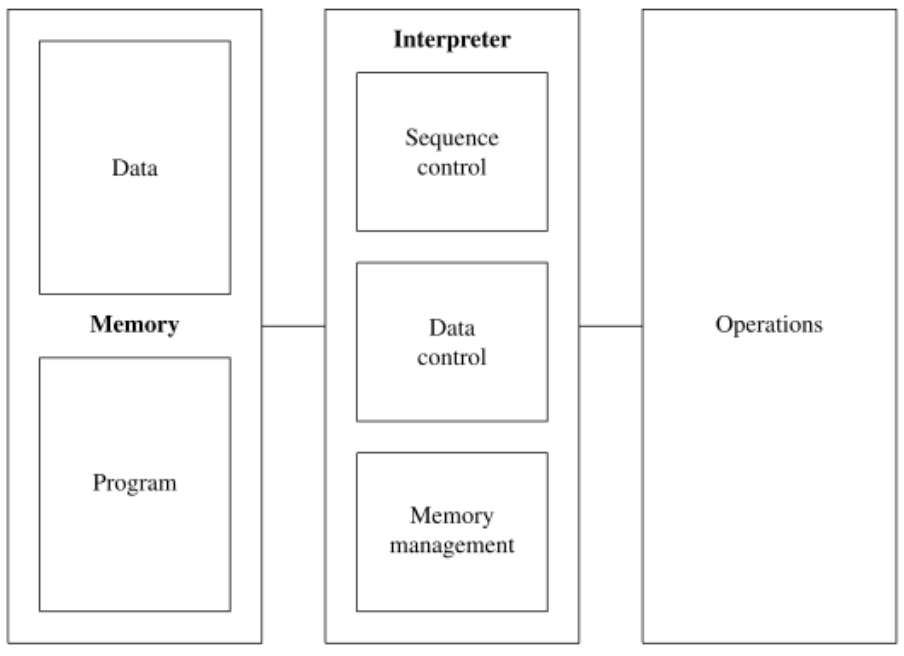
\includegraphics[scale=0.8]{img/am.png}
  % By M. Gabbrielli and S. Martini - M. Gabbrielli and S. Martini, "Abstract Machines", Undergraduate Topics in Computer Science, pp. 1-25, 2010. Available: 10.1007/978-1-84882-914-5_1., CC BY-SA 4.0, https://commons.wikimedia.org/w/index.php?curid=118069333
\end{center}

\subsubsection{Macchina di von Neumann}
Come accennato prima, l'architettura di von Neumann e' un modello semplice ma estremamente flessibile per la reallizzazione di macchine.

\begin{center}
  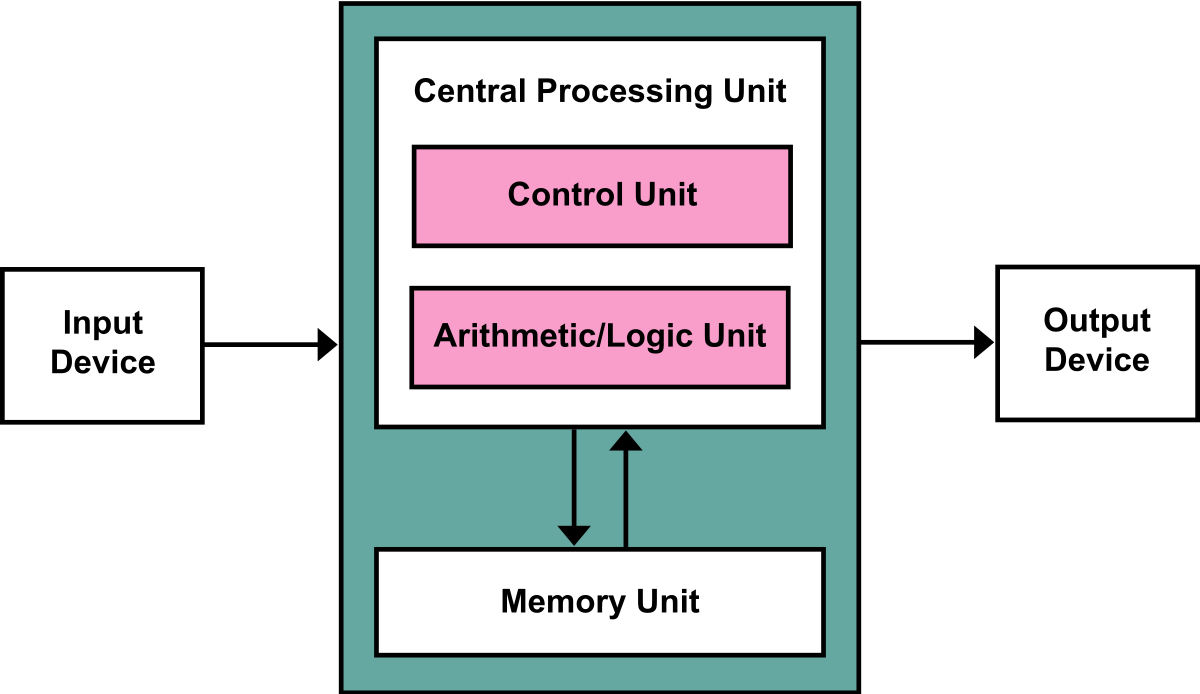
\includegraphics[scale=0.2]{img/vonneumann.png}
\end{center}

E' un modello ben adatto alla programmazione imperativa, ed e' spesso usata come base concettuale per le macchine astratte imperative. Cio' e' dovuto al concetto di "istruzione" (intrinseca al modello di von Neumann), ovvero operazioni che vengono eseguite in modo sequenziale dall' \textbf{interprete}.

\subsubsection{Interprete}
\label{interp}
L'\textbf{interprete} e' la componente fondamentale che da' alla macchina la capacita' di eseguire programmi. E' un semplice algoritmo, anche chiamato ciclo \textit{fetch-decode-execute}, che permette la corretta esecuzione delle istruzioni, coordinando le componenti della macchina astratta finche' non viene eseguita l'istruzione primitiva di arresto, che provoca l'uscita dal ciclo e l'arresto della macchina

\begin{center}
  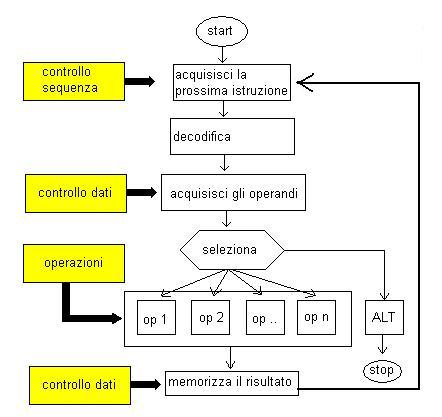
\includegraphics[scale=0.7]{img/interprete.jpg}
\end{center}

Come si vede dall'immagine, l'interprete e' costituito da operazioni e strutture dati che servono per: (implementazione nelle macchine fisiche)
\begin{itemize}
  \item Elaborare dati primitivi (ALU)
  \item Controllo sequenza di esecuzione (PC e salti)
  \item Controllo dati (Metodi di indirizzamento e trasferimento di blocchi ecc.)
\end{itemize}

La struttura dell'interprete \red{rimane invariata per qualsiasi macchina astratta imperativa}, cambiano le altre componenti.

\subsection{Linguaggio Macchina}
Data una macchina astratta $ M $, chiamiamo $ L_M $ il \textbf{Linguaggio Macchina di M}, ovvero l'insieme delle istruzioni che la macchina $ M $ e' in grado di "comprendere". Per chi programma, il linguaggio che si usa per creare programmi eseguibili da una macchina astratta e' semplicemente una sequenza di caratteri. Mentre all'interno della macchina stessa il programma viene trasformato da algoritmi, che possono sfruttare diverse strutture dati, per diventare un linguaggio comprensibile da una macchina astratta di livello piu' basso, o direttamente dalla macchina fisica (se $ M $ e' realizzata da hardware).

\section{Gerarchie di Macchine Astratte e Linguaggi}
Proviamo a costruire una macchina astratta $ M_\mathcal{L} $ che e' in grado di comprendere ed eseguire istruzioni complesse di un linguaggio $ \mathcal{L} $ di alto livello, partendo da zero. Prima di tutto, vediamo in generale come si forma la gerarchia di macchine astratte:

\subsection{Macchina Hardware}
Per prima cosa dobbiamo per forza partire dal \textbf{livello fisico}, dato che ci serve dell'hardware per eseguire il nostro programma automaticamente. Rimanendo sulla strada di macchine imperative, possiamo utilizzare l'architettura di von Neumann per progettare il sistema. Dobbiamo pero' pensare al linguaggio che l'interprete fisico deve riuscire ad eseguire: teoricamente, sarebbe possibile architettare direttamente un interprete fisico che riesca a comprendere il nostro linguaggio di alto livello, ma questo sarebbe davvero molto costoso e' difficile da implementare, quindi evitiamo. Scegliamo allora una serie di istruzioni basiche, del tipo:
\begin{itemize}
  \item \textbf{Operazioni primitive}: operazioni aritmetico logiche, manipolazione bit, I/O
  \item \textbf{Controllo sequenza}: salti (condizionali), chiamate di subroutine e strutture dati per punti di ritorno di sottoprogrammi
  \item \textbf{Controllo dati}: acquisizione di operandi e memorizzazione dei risultati
    \begin{itemize}
      \item Architettura a registri $ \to $ registri indice e indirizzamento indiretto
      \item Architettura a pila $ \to $ gestione pila
    \end{itemize}
  \item \textbf{Gestione memoria}: 
    \begin{itemize}
      \item Architettura a registri $ \to $ nessuna (memoria statica)
      \item Architettura a pila $ \to $ allocazione e recupero dati sulla pila
    \end{itemize}
\end{itemize}

A seconda del livello di complessita' delle singole istruzioni, possiamo dire che la nostra macchina fisica sia:
\begin{itemize}
  \item \textbf{RISC} (Reduced Instruction Set Computers): istruzioni semplici e solitamente poche
  \item \textbf{CISC} (Complex Instruction Set Computers): istruzioni complesse e solitamente tante
\end{itemize}

L'insieme di queste istruzioni si chiama \textbf{linguaggio macchina}.

\subsection{Macchina Microprogrammata}
A volte, nelle macchine hardware di tipo CISC, e' piu' conveniente creare col \textbf{firmware} una macchina astratta che sta sopra il livello hardware e che interpreti le istruzioni macchina. La \textbf{macchina microprogrammata} traduce queste istruzioni in istruzioni piu' semplici ($ \mu $istruzioni) che puo' eseguire l'interprete della macchina hardware ($ \mu $interprete).

Notare che la macchina microprogrammata deve essere per forza scritta in un linguaggio compreso dal livello inferiore.

\subsection{Macchina Software}
A questo punto possiamo scrivere una macchina astratta utilizzando il linguaggio fornito dalla macchina sottostante. Facciamo cio' per implementare algoritmi e strutture dati piu' complesse, che possono servire anche ai livelli superiori.

Solitamente, dopo il livello hardware (o firmware se c'e'), si trova il livello del Sistema Operativo. La macchina astratta di questo livello e' scritta in linguaggio macchina ed estende le capacita' del livello sottostante implementando primitive di livello piu' alto non presenti al livello hardware (come la gestione file). Tale macchina e' conosciuta come la \textbf{host machine} (macchina ospite o MO).

Partendo dalla macchina ospite possiamo implementare finalmente il nostro linguaggio di alto livello, creando direttamente una macchina astratta che lo riconosce (che sia eseguibile dal Sistema Operativo) o utilizzando una macchina intermediaria, possiamo anche tradurre il linguaggio in uno di livello piu' basso usando un compilatore.

\begin{center}
  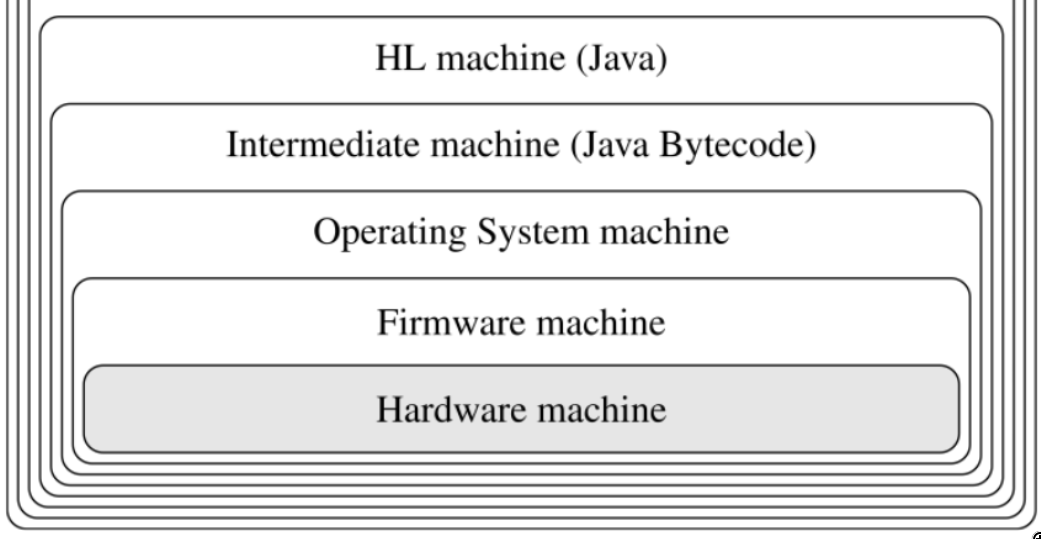
\includegraphics[scale=0.3]{img/2024-12-11-20-16-47.png}
\end{center}

\section{Implementare un linguaggio: Interpreti e Compilatori}
Ora che abbiamo capito come funziona la gerarchia di macchine astratte che ci permette di creare linguaggi di alto livello, definiamo in modo formale il processo:

\subsection{Definizione di programma}
Vogliamo imlementare un linguaggio $ \mathcal{L} $ (cioe' realizzare una macchina astratta $ M_\mathcal{L} $) partendo da una macchina ospite $ M_{\mathcal{L}_O} $. Prima di tutto, definiamo cosa sia un programma scritto in un linguaggio:
\dfn{Programma}{
  $\mathcal{P}_r^\mathcal{L}$ indica un programma $ \mathcal{P}_r $ scritto in un linguaggio $ \mathcal{L} $. 

  A $ \mathcal{P}_r^\mathcal{L} $ e' associata una funzione parziale $ \mathcal{P}^\mathcal{L} $:
  \[
    \mathcal{P}^\mathcal{L}: D \multimap \mspace{-2mu} \to D
  \]
  Dove $ D $ e' l'insieme di dati (se $ \mathcal{P}^\mathcal{L} $ non e' definita per un certo $ d \in D $, allora il programma non termina per quell'input). Tale funzione descrive la \textbf{semantica} del programma $ \mathcal{P}_r^\mathcal{L} $.
}
\nt{
  Per programmi concorrenti la questione e' piu' delicata.
}

Esistono due modi radicalmente diversi per implementare un programma:

\subsection{Implementazione interpretativa pura}
Come abbiamo visto all'inizio del capitolo (\ref{interp}), l'interprete e' la parte fondamentale delle macchine astratte. Quindi, se costruiamo un interprete per un linguaggio $ \mathcal{L} $ usando software scritto con il linguaggio $ \mathcal{L}_O $ della macchina ospite, abbiamo essenzialmente creato una nuova macchina astratta $ M_\mathcal{L} $ sopra a $ M_O $. 

\begin{center}
  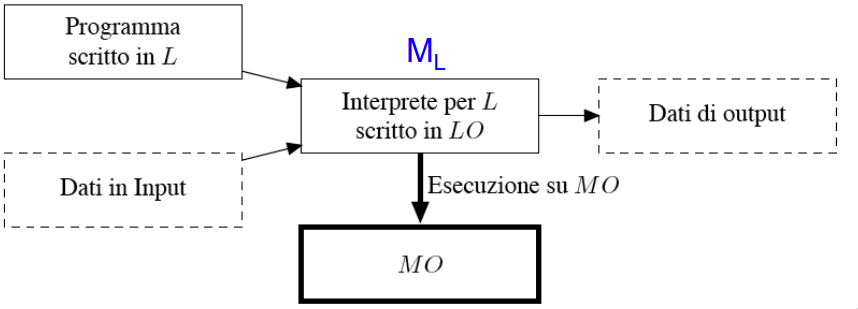
\includegraphics[scale=0.5]{img/2024-12-14-12-08-05.png}
\end{center}

Diamo ora una definizione piu' formale di interprete come funzione (senza interessarci degli aspetti implementativi):
\dfn{Interprete}{
  Un interprete nel lingauggio $ \mathcal{L} $, scritto nel linguaggio $ \mathcal{L}_O $, e' un programma che realizza la funzione parziale:
  \[
    I_\mathcal{L}^{\mathcal{L}_O}: (Prog_\mathcal{L} \times D) \multimap \mspace{-2mu} \to D
  \]
  tale che:
  \[
    I_\mathcal{L}^{\mathcal{L}_O}(\mathcal{P}_r^{\mathcal{L}}, Input) = \mathcal{P}^\mathcal{L}(Input)
  \]
}
Ovvero l'interprete \red{calcola la corretta semantica} del programma scritto nel nostro linguaggio $ \mathcal{L} $.

\subsection{Implementazione compilativa pura}
Oltre all'implementazione interpretativa, esiste un altro modo per rendere un nuovo linguaggio eseguibile su una macchina ospite, che non ha bisogno di creare una nuova macchina astratta (e quindi un nuovo interprete). L'implementazione compilativa si basa sulla \textbf{traduzione} del linguaggio nuovo $ \mathcal{L} $ in un linguaggio riconosciuto da una macchina di livello piu' basso.

\begin{figure*}
  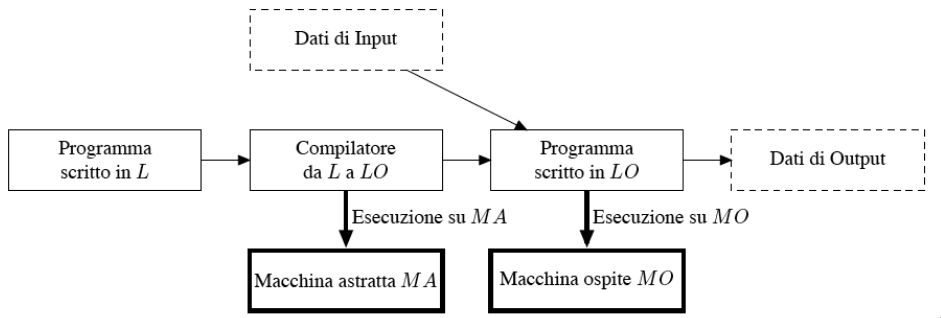
\includegraphics[scale=0.5]{img/2024-12-14-12-09-34.png}
  \caption{Nota: $ M_A $ puo' benissimo coincidere con $ M_O $}
\end{figure*}

Per eseguire tale traduzione, viene usato un programma chiamato \textbf{compilatore}, che puo' essere scritto in un qualunque linguaggio riconosciuto dalle macchine astratte del calcolatore. Il compilatore, quindi, traduce programmi scritti nel linguaggio $ \mathcal{L} $ in nuovi programmi \red{equivalenti} scritti in $ \mathcal{L}_O $:
\dfn{Compilatore}{
  Un compilatore da $ \mathcal{L} $ a $ \mathcal{L}_O $ scritto in un linguaggio $ \mathcal{L}_A $ e' un programma che realizza una funzione:
  \[
    C_{\mathcal{L}, \mathcal{L}_O}^{\mathcal{L}_A}: Prog_\mathcal{L} \to Prog_{\mathcal{L}_O}
  \]
  tale che, dato
  \[
    C_{\mathcal{L}, \mathcal{L}_O}^{\mathcal{L}_A}(P_r^\mathcal{L}) = Pc^{\mathcal{L}_O}_r
  \]
  allora, $ \forall $ Inupt $ \in D $:
  \[
    P^\mathcal{L}(Input) = Pc^{\mathcal{L}_O}_r(Input)
  \]
}
Ovvero il compilatore \red{preserva la semantica} del programma: il programma originale e quello tradotto calcolano la stessa funzione: $ P^\mathcal{L} = Pc^{\mathcal{L}_O} $.

\subsection{Differenze}
Vediamo i pro e i contro dei due metodi:
\begin{itemize}
  \item \textbf{Interprete}
    \begin{center}
      \begin{tabular}{ l | l  }
        Pro & Contro \\
        \hline
        - Flessibile (debugging facile) & - Scarsa efficenza (decodifica per ogni esecuzione) \\
        - Piu' facile da realizzare & \\
        - Occupa meno memoria & 
    \end{tabular}
    \end{center}
  \item \textbf{Compilatore}
    \begin{center}
      \begin{tabular}{ l | l  }
        Pro & Contro \\
        \hline
        - Buona efficenza & - Scarsa flessibilita' \\
        - Piu' facile da realizzare & - Perdita di info (astrazione) del programma sorgente (debuggin difficile) \\
        & - Occupa piu' memoria (non molto rilevante oggi) 
      \end{tabular}
    \end{center}
\end{itemize}

Per riuscire a combinare l'efficenza dei compilatori con la portabilita' dei linguaggi interpretati, nella realta' si utilizza spesso una via di mezzo. Solitamente:
\begin{itemize}
  \item Alcune istruzioni (es. ingresso/uscita) sono sempre \textbf{simulate} (interpretate)
  \item I programmi vengono \textbf{tradotti} in un codice intermedio
\end{itemize}

\begin{center}
  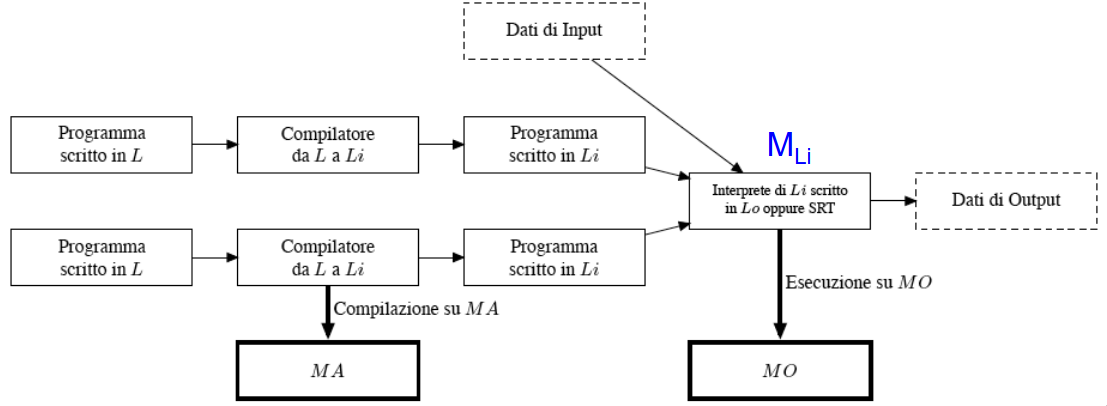
\includegraphics[scale=0.4]{img/2024-12-14-17-02-00.png}
\end{center}

Come si vede nell'immagine, il linguaggio $ L $ viene prima tradotto nel linguaggio intermedio $ L_i $, che poi viene interpretato dall'interprete di $ M_{L_i} $ scritto in $ L_O $. In base a quanto e' diverso l'interprete $ L_i $ da $ L_O $, abbiamo due implementazioni diverse:
\begin{itemize}
  \item Interpretativa: l'interprete della macchina intermedia $ M_{L_i} $ e' sostanzialmente diverso dall'interprete della macchina ospite $ M_{L_O} $. (Es. Java)
  \item Compilativa: $ M_{L_i} = M_{L_O} +  $ opportuni meccanismi, come I/O, gestione memoria, ecc. (Es. C)
\end{itemize}

\subsubsection{Cosa interpretare e cosa compilare}

Abbiamo visto che le soluzioni di tipo compilative sono piu' effcenti, mentre quelle di tipo interpretativo privilegiano flessibilita' e portabilita'. In linea di principio:
\begin{itemize}
  \item Traduzione per i costrutti di $ L $ che corrispondono da vicino a costrutti di $ L_O $
  \item Simulazione per gli altri
\end{itemize}

\subsection{Generazione Compilatori}

Ora che abbiamo esplorato i modi per eseguire programmi scritti in un linguaggio nuovo usando compilatori e interpreti, vediamo come costruire questi ultimi strumenti.

\subsubsection{Si possono sempre realizzare?}
Immaginiamo un interprete e un compilatore scritti nello stesso linguaggio $ L_{osp} $ e che ricevono in input lo stesso linguaggio $ L_{sorg} $. L'interprete e' in grado di calcolare la semantica del programma in input usando $ L_{osp} $ e il compilatore preserva la semantica del programma tradotto, quindi tutte le funzioni che $ L_{sorg} $ puo' calcolare possono essere simulate o tradotte con $ L_{osp} $. Quindi:
\[
L_{osp} \text{ e' non meno espressivo di } L_{sorg}
\]
Dato che, come vedremo piu' avanti, tutti i linguaggi di programmazione "veri" \red{sequenziali} sono ugualmente espressivi (Turing-completi, se forniti di memoria "illimitata"), allora sappiamo che questa condizione vale sempre (se $ L_{osp} $ e' un "vero" linguaggi sequenziale).

\nt{
  Esistono formalismi/linguaggi molto meno espressivi ma che sono utilissimi per la loro efficenza, come ad esempio:
  \begin{itemize}
    \item Automi finiti (analizzatori lessicali)
    \item Automi a pila (analizzatori sintattici)
  \end{itemize}
}

\subsubsection{Come viene generato un compilatore?}

Esistono diversi modi per creare un compilatore/interprete dato un linguaggio $ L $:
\begin{itemize}
  \item \textbf{Strumenti automatici}
    \begin{itemize}
      \item \textbf{Lex}: generatore di analizzatori \textbf{lessicali}
      \item \textbf{Yacc}: generatore di analizzatori \textbf{sintattici}
    \end{itemize}
    Data una descrizione formale della sintassi di $ L $, questi strumenti sono in grado di generare automaticamente un programma che riesce a riconoscere stringhe sintatticamente legali.
  \item \textbf{Implementazione via Kernel}

    Si sceglie $ H \subset L $, ovvero un sottoinisieme proprio di $ L $ che forma un nucleo (kernel) con il quale possiamo costruire:
    \begin{itemize}
      \item $ C^H_{L, L_O} $, ovvero un compilatore scritto in $ H $ che traduce $ L $ in $ L_O $, oppure
      \item $ I^H_L $, ovvero un interprete per $ L $ scritto in $ H $
    \end{itemize}
    Manca poi scrivere un interprete/compilatore per $ H $, in modo da poter eseguire uno di questi due sulla macchina ospite, che se $ H $ e' stato scelto bene non dovrebbe essere troppo difficile.

    Implementare prima un sottoinsieme di $ L $ porta a dei vantaggi:
    \begin{itemize}
      \item Semplifica l'implementazione, dato che $ H $ e' piu' vicina a $ L $ rispetto a $ L_O $
      \item Facilita la portabilita, perche' basta re-implementare $ H $ nel nuovo linguaggio macchina
    \end{itemize}
  \item \textbf{Bootstrapping}

    Immaginiamo di aver creato i seguenti compilatori e interprete, dove $ M_i $ e' una macchina astratta intermedia:
    \begin{itemize}
      \item $ C^{L_i}_{L, L_i} $
      \item $ I^{L_O}_{L_i} $
      \item $ C^L_{L, L_O} $
    \end{itemize}
    Otteniamo un compilatore per $ L $ scritto in $ L_O $ in questo modo:
    \[
      I^{L_O}_{L_i}(C^{L_i}_{L, L_i}, C^L_{L, L_O}) = C^{L_i}_{L, L_O}
    \]
    \[
      I^{L_O}_{L_i}(C^{L_i}_{L, L_O}, C^L_{L, L_O}) = C^{L_O}_{L, L_O}
    \]
    Piu' efficente rispetto al kernel, dato che abbiamo un compilatore che compila direttamente al linguaggio di $ M_O $ senza usare un linguaggio intermedio.

\end{itemize}

\chapter{Introduzione ai linguaggi normali: grammatiche}


\section{Linguaggi (naturali o artificiali)}

La descrizione di un linguaggio avviene su 3 dimensioni:
\begin{itemize}
    \item \textbf{Sintassi}: regole di formazione, ovvero la relazione tra segni
    \item \textbf{Semantica}: attribuzione di significato
    \item \textbf{Pragmatica}: in quale modo frasi corrette e sensate sono usate
    \item \textbf{Implementazione}: come eseguire una frase corretta rispettandone la semantica
\end{itemize}

Partiamo con il descrivere questi elementi

\subsection{Sintassi}

\dfn{sintassi}{La \textbf{sintassi} è la parte della grammatica che studia la struttura delle frasi e il modo in cui le parole si combinano per formare enunciati corretti e significativi}


Si dirama in diversi aspetti: 
\begin{itemize}
    \item \textbf{Aspetto lessicale} che riguarda le parole che si possono usare, quindi:
    \begin{itemize}
        \item descrizione del lessico, intuitivamente i dizionari per i linguaggi naturali assolvono a questo compito
        \item errori dovuti a vocaboli inesistenti
    \end{itemize}
    \item \textbf{Aspetto grammaticale} che si riferisce nel modo in cui è possibile costruire frasi corrette è possibile cotruire con il lessico. Le frasi grammaticalmente corrette possono essere costruite grazie all'uso delle regole grammaticali, che sono in numero finito, mentre il numero di frasi generabili è infinito.
    
    Un errore grammaticale è una frase scorretta, anche se il lessico utilizzato è corretto. Es. "La cane abbaiano"
\end{itemize}

\subsection{Semantica}
\dfn{Semantica}{La \textbf{semantica} è la branca della linguistica che studia il significato delle parole, delle frasi e degli enunciati}

\begin{itemize}
    \item \red{Per il lessico} (quindi lo studio e il significato delle parole) bastano \red{i dizionari}
    \item \red{Per le frasi} è più complicato, \red{devo sapere} infatti:
    \begin{enumerate}
        \item a \red{quale linguaggio appartiene la frase}
        \item su \red{quale linguaggio basarmi per dare significato}
    \end{enumerate}
\end{itemize}

\begin{center}

    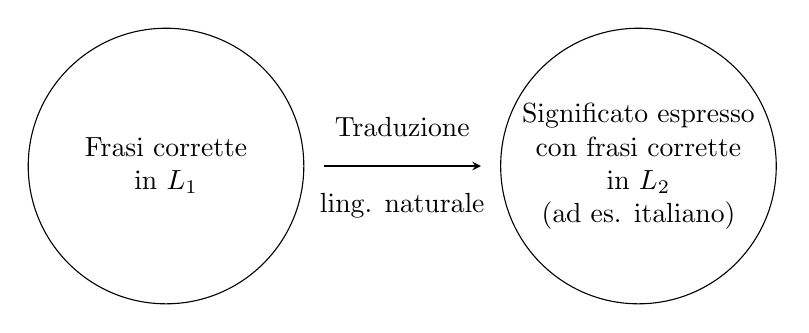
\begin{tikzpicture}
        % Primo cerchio (Frasi corrette in L1)
        \draw (0,0) circle (1.75cm);
        \node at (0,0) {\begin{tabular}{c}
                         Frasi corrette \\ 
                         in \textit{$L_1$}
                         \end{tabular}};
                         
        % Secondo cerchio (Significato espresso con frasi corrette in L2)
        \draw (6,0) circle (1.75cm);
        \node at (6,0) {\begin{tabular}{c}
                         Significato espresso \\ 
                         con frasi corrette \\ 
                         in \textit{$L_2$} \\ 
                         (ad es. italiano)
                         \end{tabular}};
        
        % Freccia tra i due cerchi
        \draw[->] (2,0) -- (4,0);
        \node at (3,0.5) {Traduzione};
        \node at (3,-0.5) {ling. naturale};
    \end{tikzpicture}
\end{center}
\begin{center}
    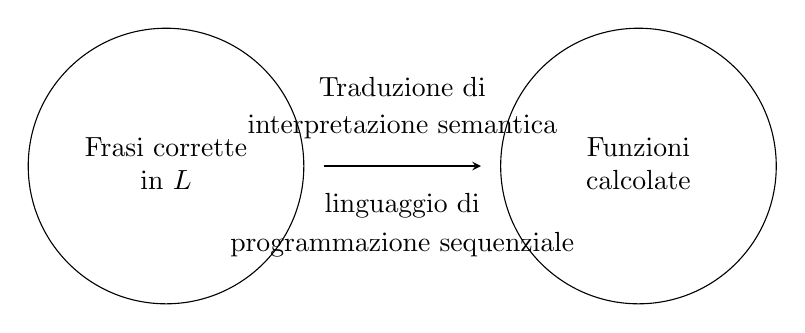
\begin{tikzpicture}
        % Primo cerchio (Frasi corrette in L1)
        \draw (0,0) circle (1.75cm);
        \node at (0,0) {\begin{tabular}{c}
                         Frasi corrette \\ 
                         in \textit{$L$}
                         \end{tabular}};
                         
        % Secondo cerchio (Significato espresso con frasi corrette in L2)
        \draw (6,0) circle (1.75cm);
        \node at (6,0) {\begin{tabular}{c}
                         Funzioni \\ 
                         calcolate \\ 
                         \end{tabular}};
        
        % Freccia tra i due cerchi
        \draw[->] (2,0) -- (4,0);
        \node at (3,1) {Traduzione di};
        \node at (3,0.5) {interpretazione semantica};
        \node at (3,-0.5) {linguaggio di};
        \node at (3,-1) {programmazione sequenziale};
    \end{tikzpicture}
\end{center}

\subsection{Pragmatica}
\dfn{Pregmatica}{
    La \textbf{pragramtica} è un insieme di regole che guidano l'uso e come i contesti influiscono sull'interpretazione di frasi sensate e corrette
}
Ad esempio quando e a chi dare del "tu" o del "lei" quando ci rivolgiamo a delle persone

\subsection{Implementazione}
L'implementazione è \red{l'esecuzione di una frase sintatticamente corretta rispettandone la semantica}

%todo   FINIRE LA FIGURA (ZIO PERA)

\begin{tikzpicture}
    \draw(0,0) circle (1cm);
    
\end{tikzpicture}

La semantica di $P$, è la funzione $f$ che è pure la semantica del programma compilato $Q$, quindi l'implementazione $Q$ di $P$ preseva la semantica di $P$!

\section{Lessico e frasi di un linguaggio}
Innanzi tutto diamo tre definizioni
\dfn{alfabeto}{
    Un \textbf{alfabeto} è un insieme (tipicamente) finito i cui elementi sono detti simboli 
}
Definire l'alfabeto ci porta alla definizione di lessico:
\dfn{Lessico}{
    Il \textbf{lessico} è un insieme di sequenze finite costituite con caratteri o simboli dell'alfabeto
}
Il quale ci porta alla fenizione di frase:
\dfn{frase}{
    Una \textbf{frase} è un insieme sequenze finite contruite con parole del lessico. 
}
È, quindi, facile notare che \red{il lessico è un alfabeto per le frasi}

Si ci si può ora astrarre e definire un linguaggio formale:
\dfn{linguaggio formale}{
    Un \textbf{linguaggio formale} $L$ su alfabeto $A$ è un sottoinsieme di $A^*$ ($L\subseteq A^*$), dove:
    \[
        A^* = \bigcup_{n \geq 0} A^n \quad \text{ dove } A^0 =\{\epsilon\}       
    \]
    e \[
        A^{n+1}= A\cdot A^n \quad n\geq 0    
    \]
    con $A\cdot A^n = \{aw|a\in A \land w \in A^n\}$
}
Si osservi che \red{$A^*$ è un insieme infinito contabile} dato un ordinamento $ < $ sui simboli di $A$, possiamo elencare tutt le parole come segue:
\begin{enumerate}
    \item elenco la parola vuota $\epsilon$ ($A^0$)
    \item poi elenco le parole di lunghezza 1 ($A^1$) secondo l'ordinamento $ < $
    
    Es. $a,b,c,\dots$
    \item poi elenco le parole in $A^2$ secondo $ < $
    
    Es. $aa, ab, ac, \dots, ba, bb, bc, \dots$
    \item così via
\end{enumerate}

Anche se l'alfabeto $A$ fosse infinito (quindi $A=\{a_0, a_1, \dots\}$) $A^*$ sarebbe ancora contabile, ovvero esisterebbe la possibilità di elencare tutte le possibili parole in $A^*$. Infatti, \red{esiste una biezione tra $A$ e $\mathbb{N}$} e riguardo ai numeri naturali si sa che:
\begin{itemize}
    \item $\mathbb{N}\times \mathbb{N}$ (prodotto cartesiano) è numerabile. La dimostrazione viene fatta attraverso il \textit{dove-tailing}, una tecnica comune per dimostrare la numerabilità di coppie di numeri naturali. Questa dimostrazione introduce la cosìdetta \textbf{funzione di decodifica}
    
    \[
        f^2(x_1,x_2) =\frac{(x_1+x_2)(x_1+x_2+1)}{2} + x_2
    \]
    che presi due numeri in $\mathbb{N}$ completa la seguente tabella ordinando i numeri naturali in "diagonale"
    
    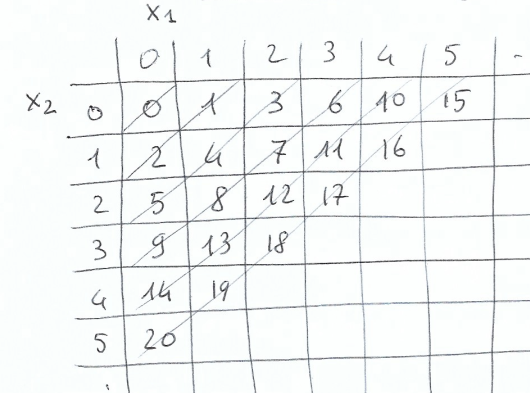
\includegraphics[width=10cm]{funzione-decodifica-tabella.png}

    è pertanto vero, quindi, che
    \[
        f^2:\mathbb{N}\times \mathbb{N}\to \mathbb{N}
    \]
    è biunivoca

    \item $\mathbb{N}^k$ è numerabile. Infatti si può dimostrare attraverso questo algoritmo:
    \[
        f^k(x_1,x_2,\dots,x_k) = \text{ if } (k=2) \text{ then } f^2(x_1,x_2)
        \quad \text{ else } f^2(x_1, f^{k-1}(x_2,\dots,x_k))
    \]
    Ovvero riduce una funzione con $k$ variabili nel dominio ad una serie di funzioni matrioska per ricondurla alla forma $f^2:\mathbb{N}\times\mathbb{N}\rightarrow \mathbb{N}$
    \item $\mathbb{N}^* = \bigcup_{k\geq 0}\mathbb{N}^k$ è numerabile. Infatti:
    \[
        f(x_1,\dots,x_k) = f^2(k,f^k(x_1,\dots, x_k))    
    \]

    
\end{itemize}

\section{Notazioni e definizioni ausiliarie}
Vengono riportate qui alcune definizioni/notazioni
\subsection{Lunghezza}
\dfn{lunghezza}{
    La \textbf{lunghezza} di una parola o stringa è definita per induzione così:
    \begin{itemize}
        \item Caso $|\epsilon|$: $0$
        \item Caso $|aw|$: $1 + |w|$
    \end{itemize}
}
Es: $|abc|=2$ 
\subsection{Concatenazione}
\dfn{Concatenazione}{
    La \textbf{concatenazione} $xy$ tra una stringa $x$ e $y$, è la parola ottenuta giustapponendo $x$ e $y$. Formalmente:
    \[
        w = xy \iff \begin{cases}
            |w|=|x|+|y| \\
            w(j) = x(j) & \text{ per } 1\leq j\leq |x|\\
            w(|x|+j) = x(j) & \text{ per } 1\leq j\leq |y|
        \end{cases}    
    \] 
    Dove $w(j)$ indica il j-esimo simbolo di $w$
}

Questi sono le leggi della concatenazione
\begin{itemize}
    \item Associatività: $x(yz)=(xy)z$
    \item Elemento neutro ($\epsilon$): $x\epsilon = x = \epsilon x$
\end{itemize}

\subsection{Sottostringa}
\dfn{Sottostringa}{
    La stringa $v$ si dive \textbf{sottostringa} di $w \iff \exists x,y \in A^*$ t.c. $w=xvy $ dove $x$ e $y$ possono essere $\epsilon$
}
Si osservi, quindi, che:
\begin{itemize}
    \item Ogni stringa è sottostringa di se stessa
    \item $\epsilon$ è sottostringa di ogni stringa
\end{itemize}

\subsection{Suffisso}
\dfn{suffisso}{
    $v$ si dice \textbf{suffisso} di $w \iff \exists x \in A^x. w=xv$
}
\subsection{Prefisso}
\dfn{prefisso}{
    $v$ si dice \textbf{prefisso} di $w \iff \exists x \in A^x. w=vx$
}
\subsection{Potenza n-esima}
\dfn{potenza n-esima}{
    Si dice \textbf{potenza n-esima} di una stringa $w$ il valore $n\geq 0$ il cui significato è definito per induzione:
    \begin{itemize}
        \item Caso 0: $w^0 = \epsilon$
        \item Caso $n+1$: $w^{n+1}= ww^{n}$
    \end{itemize}
}


\subsection{Linguaggio}
\dfn{linguaggio}{
    Si dice \textbf{linguaggio $L$ su alfabeto $A$} un sottoinsieme $L\subseteq A^*$
}
Vengono riportati qui alcuni esempi
\esempio{
    Se $A=\{a\}$, si possono avere:
    \begin{itemize}
        \item $\emptyset,\{\epsilon\}, \{a,aaa\}$ sono linguaggi finiti
        \item $L_1=\{a^n|\geq 1\}=\{a,aa,aaa,\dots\}=A^*\diagdown \{\epsilon\} $ 
        \item $L_2 =\{a^{2n}|n\geq 0\}=\{\epsilon, aa, aaaa\}$
    \end{itemize}
}
%adssad
\section{Operazione sui linguaggi}
Qui sono elencati le varie operazioni
\subsection{Complemento}
\dfn{complemento}{
    È definito \textbf{complemento} il linguaggio completare ad un linguaggio $L$, ovvero:
    \[
        \overline{L} = \{w\in A^* | w \notin L\} = A^*\diagdown L    
    \]
}
\subsection{Unione e intersezione}
\dfn{unione e intersezione}{
    Ovvi:
    \[
      \begin{array}{l}
            L_1\cup L_2 \{w|w\in L_1 \lor w \in L_2\} \\
            L_1\cap L_2 \{w|w\in L_1 \land w \in L_2\}
      \end{array}
    \]
}

\subsection{Concatenazione}
\dfn{concatenazione}{
    
        È definita \textbf{concatenazione} tale operazione:
        \[
            L_1 \cdot L_2 =\{w_1w_2|w_\in L_1 \land w_2 \in L_2\}
        \]
    
}
Ecco alcuni esempi:
\esempio{
    \begin{itemize}
        \item $L_1 = \{a^n \mid n > 0 \}$ \quad $L_2 = \{b\}$ \\
              $L_1 \cdot L_2 = \{a^n b \mid n > 0\}$
              
        \item $L_1 = \{a^{2n} \mid n > 0 \}$ \quad $L_2 = \{b^m \mid m > 0\}$ \\
              $L_1 \cdot L_2 = \{a^{2n} b^m \mid n, m > 0\}$
              
        \item $L_1 = \{a^m b^n \mid n > 0\}$ \quad $L_2 = \{b^m \mid n > 0\}$ \\
              $L_1 \cdot L_2 = \{a^m b^{n+m} \mid n, m > 0\}$ \\
              \phantom{$L_1 \cdot L_2$} $= \{a^m b^n \mid m \geq n > 0\}$
              
        \item $L_1 = \{a^m \mid m > 1 \}$ \quad $L_2 = \{a^m b^m \mid n > 0 \}$ \\
              $L_1 \cdot L_2 = \{a^{m+n} b^m \mid m > 1, m > 0\}$ \\
              \phantom{$L_1 \cdot L_2$} $= \{a^m b^m \mid m > m > 0\}$
              
        \item $L_1 = \{a b^m \mid n \geq 1\}$ \quad $L_2 = \{a, c\}    \cup \{b^n \mid n \geq 1\}$ \\
              $L_1 \cdot L_2 = \{a b^m a \mid m \geq 1\} \cup \{a b^m c \mid n \geq 1\}$ \\
              \phantom{$L_1 \cdot L_2$} $\cup \{a b^n \mid n \geq 2\}$
              
        \item $A = \{0,1\}$ \\
              $L_1 = \{ w \in A^* \mid w \text{ contiene un numero pari di "0"} \}$ \\
              $L_2 = \{ w \in A^* \mid w = 0y \text{ e } y \in \{1^*\} \}$ \\
              $L_1 \cdot L_2 = \{w \in A^* \mid w \text{ ha un numero dispari di "0"} \}$
    \end{itemize}
}
\subsection{Potenza di un linguaggio}
\dfn{Potenza di un linguaggio}{
    La \textbf{potenza di un linguaggio} viene definita per induzione:
    \begin{itemize}
        \item Caso 0: $L^0 =\{\epsilon\}$
        \item Caso $n+1$: $L\cdot L^n \quad \forall n\geq 0$ 
    \end{itemize}
}

\subsection{Stella di kleene}
\dfn{stella di kleene}{
    Si dice \textbf{stella di kleene}:
    \[
        L^* \bigcup_{n\geq 0} L^n    
    \]
    Oppure 
    \[
        L^+ =   \bigcup_{n\geq 1} L^n   
    \]
    Quest'ultima detta \textbf{chiusura positiva}
}

%asaddsadsa
\section{Definire finitamente un linguaggio}
\subsection{esempio 1: frasi palindrome}
Una frase palindroma è una parola che letta da $sx$ a $dx$ è uguale a se stessa letta da $dx$ a $sx$

Es. "I topi non avevano nipoti"
\begin{itemize}
    \item $A=\{a,b\} \quad L=\{\epsilon, a, b, aa, bb, aba, bab, \dots\}$. Come si nota è piuttosto scomodo
\item Una palindroma può essere: 
        \begin{itemize}
            \item o è la stringa $\epsilon$
            \item oppure a
            \item oppure b
            \item oppure a "palindroma" a
            \item oppure b "palindroma" b
        \end{itemize} 
    \item rappresentazione tramite \textbf{Backus-naur form (BNF)}.
    \[
         \langle P \rangle := \epsilon \mid a\mid b\mid a \langle P \rangle a\mid b \langle P \rangle b   
    \]
    \item  Come \textbf{grammatica}:
    \[
        P\to \epsilon \mid a\mid b\mid aPa\mid bPb    
    \]
    \item definizione ricorsiva in cui:
    \begin{itemize}
        \item $P$ è detto \textit{simbolo non terminale}
        \item $a,b$ sono "simboli terminali"
    \end{itemize}
\end{itemize}
\subsection{Esempio 2}
espressioni aritmetiche formate a partire dalle variabili $a$ e $b$ con gli operatori $\times, +$ e le parantesi $(,)$

Una $expr$ può essere:
\begin{itemize}
    \item \begin{itemize}
        \item la variabile $a$
        \item la variabile $b$
        \item $expr\times expr$
        \item $expr + expr$
        \item ($expr$)
    \end{itemize}
    \item \textbf{bnf}:
      \[
        \langle E \rangle ::= a\mid b\mid \langle E \rangle\times \langle E \rangle \mid \langle E \rangle + \langle E \rangle\mid (\langle E \rangle)
      \]
    \item Grammatica:
    \[
        E\to a\mid b\mid E\times E\mid E+E\mid (E)    
    \]
\end{itemize}

\section{Grammatiche} 
Una grammatica è un insieme di regole che descrivono come le parole e le frasi possono essere combinate per formare espressioni valide. Queste regole determinano la struttura sintattica di un linguaggio, specificando come le unità di base (come le parole o i simboli) si connettono per formare frasi o espressioni più complesse. Ogni grammatica \red{segue lo stesso pattern definito} differenziandosi solo per come sono caratterizzate le produzioni.

Quelle più utili sono le cosiddette grammatiche libere dal contesto (in rapporto tra facilità di analisi ed espressività) 

\dfn{grammatiche libere (dal contesto)}{ \label{dfn: gramLib}
    Una \textbf{grammatica libera} da contesto è una quadrupla $(NT,T,R,S)$ dove:
    \begin{itemize}
        \item \textbf{NT} è un insieme finito di simboli non terminali
        \item $T$ è un insieme finito di simboli terminali
        \item $S\in NT$ è detto simbolo iniziale
        \item $R$ è un insieme finito di produzione (o regole) della forma:
        \[
            V \to w \text{ dove }V\in NT \land w\in (T\cup NT)^*    
        \]
    \end{itemize}
}

Alcuni esempi:
\esempio{
    \[
        G= (\{S\}, \{a,b,+,\times\}, S, R)
    \]
    Con 
    \[
        R=\{S \to a, S \to b, S\to S+S, S\to S\times S\}    
    \]
}

\section{Derivazioni}
\dfn{derivazione immediata}{
    Data $G=(NT, T,R,S)$ libera dal contesto, diciamo che da $v$ si \textbf{deriva immediatamente}  $w$, e lo denotiamo con $v \Rightarrow w$, se:
    \[
        \frac{v =xAy \quad (A\to z )\in R \quad w=xzy}{v\Rightarrow w}    
    \]
    
}
\dfn{derivazione}{
    Diciamo che da $v$ si \textbf{deriva} $w$ (o anche "$v$ si riscrive in $w$"), e lo deontiamo con $v \Rightarrow^* w$, se esiste una sequenza finita (evenutalmente vuota) di derivazione immediate 
    \[
        v \Rightarrow w_0 \Rightarrow w_1 \Rightarrow \dots \Rightarrow w
    \]
    Cioè:
    \[
        \frac{ }{v \Rightarrow^* v} \quad \frac{v\Rightarrow^* w \quad w\Rightarrow z}{v\Rightarrow^* z}    
    \]
    Dove $\Rightarrow^*$ è la chiusa riflessiva e transitiva della relazione $\Rightarrow$
}

\section{Linguaggio Generato}
\dfn{Linguaggio Generato}{
    Il \textbf{linguaggio generato} da una grammatica $<G=(NT, T ,R,S)$ è l'insieme
    \[
        L(G) = \{w\in T^*|S \der w\}
    \]
}

\subsection{Algoritmo di Naif}

Data una grammatica $G$ è opportuno chiedersi come si fa a determinare un linguaggio $L(G)$ e a verificare se $w\in L(G)$. La domanda può essere complessa, tuttavia in casi semplici ci viene in aiuto \textbf{l'algoritmo di Naif} che consiste nel partire da $S$ e provare ad applicare in tutti i modi possibili le produzione (regole) per trovare una derivazione che generi $w$

In certi casi questa verifica è semplice

\esempio{
    \begin{itemize}
        \item 
            Sia $G_3$ con $S\to aSb|ab$

            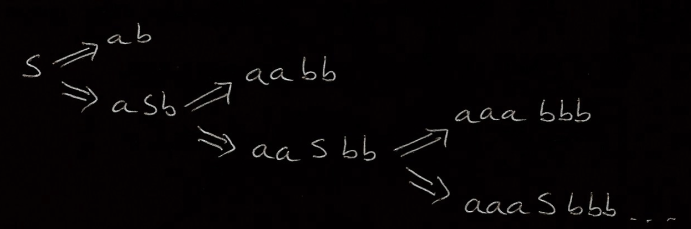
\includegraphics[width=10cm]{alberello.png}
        
            In questo esempio è facile determinare che $L(G_3)=\{a^n b^n|n\geq 1\}$
        \item 
            Sia $G_1 \to aAb \text{ e }A\to aAb\mid \epsilon$ 

            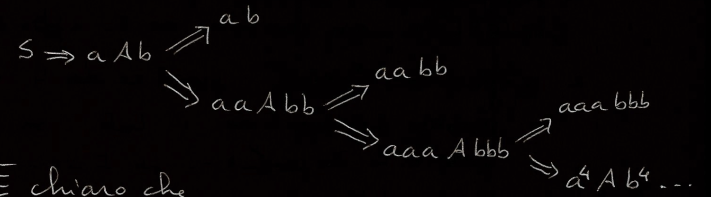
\includegraphics[width=10cm]{alberello-1.png}

            Quindi $L(G_1) = \{a^nb^n\mid n\geq 1\}$
    \end{itemize}

    Si può notare che $G_1 \text{ e } G_3$ sono grammatiche equivalenti perché $L(G_1)=L(G_3)$

    In generale \red{esistono grammatiche diverse che generano lo stesso linguaggio}
    
}

\section{Alberi di derivazione}

Per rappresentare graficamente e semplicemente una certa grammatica esiste uno strumento utilissimo, ovvero l'albero di derivazione

\dfn{albero di derivazione}{ \label{dfn: alberoDer}
    Data una grammatica libera $G= ( NT, T, S, R)$, un albero di derivazione (o di parsing) è un albero ordinato in cui: 
    \begin{itemize}
        \item Ogni nodo è etichettato con un simbolo in $NT \cup \{\epsilon \} \cup T$
        \item la radice è etichettata con $S$
        \item ogni nodo interno è etichettato con un simbolo in $NT$ 
        \item se il nodo $n$
        \begin{itemize}
            \item ha etichetta $A\in NT$ 
            \item i suoi figli sono nell'ordine $m_1,\dots, m_k$ con ,etichetta $x_1,\dots, x_k$ (in $NT\cup T$), allora
            \[
                A \to x_1, \dots , x_k \text{ è una produzione in R }
            \]
        \end{itemize}
        \item se il nodo $n$ ha etichetta $\epsilon$, allora $n$ è una foglia, è figlio unico e, dato $A$ suo padre, $A\to \epsilon$ è una produzione di $R$
        \item se inoltre ogni nodo foglia è etichettato su $T\cup\{\epsilon\}$ è una produzione di $R$
        \item se inoltre ogni nodo foglia è etichettato su $T\cup\{\epsilon\}$, allora l'alberello di derivazione corrisponde ad una derivazione completa
    \end{itemize}
}

Un albero di derivazione, quindi, \red{riassume tante derivazioni diverse ma tutte equivalenti} (ovvero generano lo stesso albero)
\esempio{
    Consideriamo la grammatica 
    \[
        s\to a|b|c|S+S|S \times S
    \]
    Inoltre si consideri la derivazione
    \[
        S \Rightarrow \underbar{S}+S \Rightarrow \underbar{S}\times S + S \Rightarrow a \times \underbar{S}+S \Rightarrow a \times b + \underbar{S} \Rightarrow a\times b + c
    \]
    Allora il suo albero di derivazione è:
    \begin{center}
        
        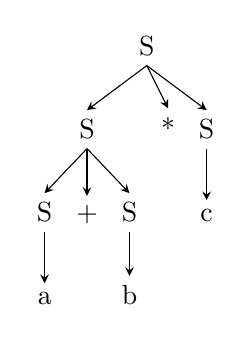
\begin{tikzpicture}
            \Tree [.S 
                    [.S [.S a ] + [.S b ] ] 
                    * 
                    [.S c ]
                ]
        \end{tikzpicture}
    \end{center}
}
Si osservi inoltre che l'albero di derivazione fornisce informazioni semantiche: "quali operandi per quali operatori" e possono essere riassunti nei cosiddetti \red{alberi sintattici}, tipo
\begin{center}
    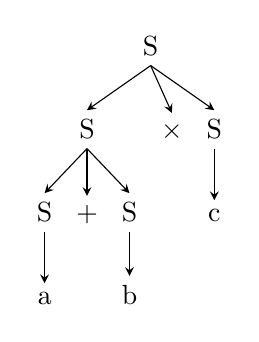
\begin{tikzpicture}
        \Tree [.S 
                [.S [.S a ] + [.S b ] ] 
                $\times$
                [.S c ]
             ]
    \end{tikzpicture}
    e
    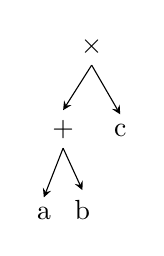
\begin{tikzpicture}
            \Tree [.$\times$ 
                    [
                        .+ 
                        [.a ] 
                        [.b ] 
                    ] 
                    [
                        .c 
                    ] 
                  ]
    \end{tikzpicture}    
\end{center}

        


\teorema{
    Una stringa $w\in T^*$ appartiene a $L(G)$ sse ammette un albero di derivazione completo (le cui foglie, lette da sx a dx diano la stringa $w$) cioè visita in ordine anticipato tralasciando i nonterminali
}


\subsection{Ambiguità}
Per generare una stringa $ w $, una grammatica libera $ G $ puo' avere diversi \textit{alberi di derivazione}, che quindi attribuiscono un significato diverso allo stesso input, vediamo un esempio:
\esempio{ \label{ex: gramAmbi}
    Si consideri la seguente grammatica
    \[
        S\to a|b|c|S+S|S\times S    
    \]
    Si hanno due diverse derivazioni per $a\times b + c$:
    \begin{enumerate}
        \item  $S \Rightarrow \underbar{S}+S \Rightarrow \underbar{S}\times S + S \Rightarrow a \times \underbar{S}+S \Rightarrow a \times b + \underbar{S} \Rightarrow a\times b + c$
        
        con l'albero: 
        \begin{center}
            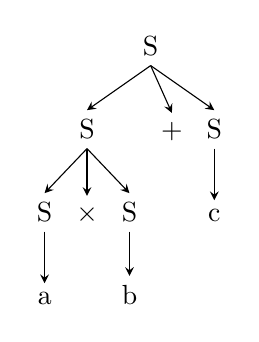
\begin{tikzpicture}
                \Tree [.S 
                        [.S [.S a ] $\times$ [.S b ] ] 
                        + 
                        [.S c ]
                    ]
            \end{tikzpicture} 
        \end{center}
        \item $S \Rightarrow \underbar{S}\times S \Rightarrow a \times \underbar{S} \Rightarrow a  \times \underbar{S} + s \Rightarrow a\times b + \underbar{S} \Rightarrow a\times b + c$
        
        Con l'albero:

        \begin{center}
            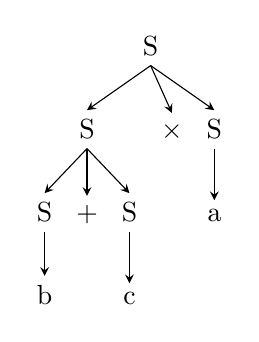
\begin{tikzpicture}
            \Tree [.S 
                [.S 
                    [.S b ] 
                    + 
                    [.S c ] 
                ]
                $\times$
                [.S a ] 
            ]
            \end{tikzpicture}
        \end{center}
    \end{enumerate}

}
Nella grammatica dell'esempio \ref{ex: gramAmbi}, la stringa $a\times b + c $ ha più di un albero di derivazione. In questi casi si dice che la grammatica è quindi \red{inutilizzabile per dare semantica a $a\times b + c $} e viene definita \textbf{ambigua}. Bisogna utilizzare grammatiche non ambigue, o manipolare grammatiche ambigue per disambiguarle.
\dfn{Grammatica ambigua}{
Una grammatica libera $G$ è \textbf{ambigua} se $\exists w \in L(G)$ che ammette più alberi di derivazione.
}
E di conseguenza:
\dfn{Linguaggio ambiguo}{
    Un linguaggio $L$ è \textbf{ambiguo} se tutte le grammatiche $G$, tali che $L(G)=L$, sono ambigue
}

Attenzione! Abbiamo detto che una grammatica e' ambigua se, per lo stesso input, ha \textit{alberi} di derivazione diversi, \textbf{NON} \textit{derivazioni} diverse. Questa distinzione e' necessaria perche' due derivazioni possono differire semplicemente nell'ordine in cui sostituisono i nonterminali, generando pero' lo stesso albero di derivazione e quindi attribuendo lo stesso significato all'input. 

\subsubsection{Derivazioni rightmost e leftmost} 
Per poter studiare l'ambiguita' di una grammatica guardando le sue derivazioni, ci e' utile fissare un'unica strategia per decidere quale nonterminale sostitiure ad ogni passaggio di derivazione. Una convenzione semplice e' quella di prendere il nonterminale piu' a sinistra (o a destra) della stringa intermedia di derivazione. Queste due strategie si chiamano derivazioni \textit{leftmost} e \textit{rightmost}:
\dfn{Derivazione leftmost (e rightmost)}{ 
  Sia $ G = (NT, T, R, S) $ una grammatica libera. Diciamo che $ u \Rightarrow_l v $ se $ u = xXy, v = xzy $, dove $ x \in T^*, y \in (T \cup NT)^* $ e $ X \to z \in R $. Se, invece, $ x \in (T \cup NT)^* $ e $ y \in T^* $, allora $ u \Rightarrow_r v $. 

  Quindi, scriviamo $ u \Rightarrow_l v $ quando sostituiamo il nonterminale di $ u $ che si trova piu' a sinistra, e $ u \Rightarrow_r v $ quando sostituiamo quello piu' a destra. Detto cio', una \textbf{derivazione leftmost} e' una derivazione $ u_1 \Rightarrow^*_l u_n $ tale che:
  \[
  u_1 \Rightarrow_l u_2 \Rightarrow_l ... \Rightarrow_l u_n
  \]
  Quindi ad ogni passo sostituiamo il nonterminale piu' a sx (in modo analogo per rightmost).
}\label{dfn: derLeft}
Si puo' dimostrare che, se per una stringa $ w $ esiste un'albero di derivazione per una grammatica $ G $, allora esistono sicuramente derivazioni leftmost e rightmost di $ w $. In piu', possiamo dimostrare che i seguenti numeri sono uguali:
\begin{itemize}
  \item Il numero di derivazioni leftmost di $ w $
  \item Il numero di derivazioni rightmost di $ w $
  \item Il numero di alberi di derivazione distinti di $ w $
\end{itemize}

Detto cio', possiamo utilizzare la definizione di grammatica ambigua per arrivare alla seguente proposizione:
\mprop{Derivazioni leftmost/rightmost e ambiguita'}{
  Data una grammatica libera $ G $, questa' e \textbf{ambigua} sse $ \exists w \in L(G) $ tale che:
  \begin{center}
    $ w $ ha piu' di una derivazione leftmost/rightmost
  \end{center}
}

\subsection{Rimuovere l'ambiguità}
Alcune grammatiche possono essere manipolate di modo da \begin{itemize}
    \item rimuovere l'ambiguità
    \item generare lo stesso linguaggio
\end{itemize}
In altre, invece, ti tieni l'ambiguità (non è possibile rimuoverla (cazzo)). Questa CAZZATA viene spiegata con solo degli esempi:

\esempio{
    Sia $S$ la grammatica
    \[
        S\to a\mid b\mid c\mid S+S\mid S\times S \text{ è ambigua!}       
    \]
    Problemi: \begin{itemize}
        \item Precedenza del * rispetto al + in modo che $a\times b + c$ sia interpretato come:
        \begin{center}
            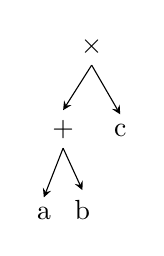
\begin{tikzpicture}
                \Tree [.$\times$ 
                        [
                            .+ 
                            [.a ] 
                            [.b ] 
                        ] 
                        [
                            .c 
                        ] 
                      ]
            \end{tikzpicture}  
        \end{center}
        \item associatività del $+$ e del $\times$
        \begin{center}
            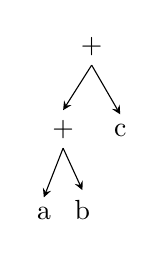
\begin{tikzpicture}
            \Tree [.+
                    [
                        .+ 
                        [.a ] 
                        [.b ] 
                    ] 
                    [
                        .c 
                    ] 
                  ]
        \end{tikzpicture}  
        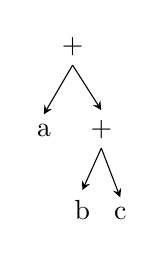
\begin{tikzpicture}
            \Tree [.+
                    [
                        .a
                    ] 
                    [
                        .+ 
                        [.b ] 
                        [.c ] 
                    ] 
                  ]
        \end{tikzpicture}  
    \end{center}
        
        $a+b+c$ ovvero bisogna scegliere l'associatività a dx o sx
        
    \end{itemize}

    Un modo per eliminare questa ambiguità è definire la grammatica così:
    \[
        e\to E+T\mid T \quad T\to A \times T\mid A \quad A \to a\mid b\mid c\mid(E)    
    \]
}

\chapter{Struttura di un compilatore, semantica statica, semantica dinamica}
\section{Vincoli contestuali}
\dfn{vincoli sintattici contestuali}{
    I \text{vincoli sintattici contestuali} sono termini o parole riservate non esprimibili per mezzo di grammatiche libere (perché non possono descrivere vincoli vincoli che dipendono dal contesto) che bisogna evitare di considerare quando si esegue il codice
}

Tradizionalmente i vincoli sintattici contestuali appartengono alla sintassi, ma nel gergo dei $LP$, si intende:
\begin{itemize}
    \item \textbf{Sintassi}: quello che si \red{scrive per mezzo di Grammatiche Libere}
    \item \textbf{semantica} tutto il resto $\dots$
\end{itemize}  

Pertanto \red{i vincoli contestuali sono dunque vincoli semantici, detti di } \textbf{semantica statica} cioè vincoli che possono essere verificati ispezionando il codice \red{senza mandare il programma in esecuzioni}

Il compilatore delega questi controlli di semantica statica alla cosiddetta \textbf{analisi semantica}
\section{Semantica statica}
\dfn{Semantica statica}{
    Per \textbf{semantica statica} si intende l'insieme di quei controlli che possono essere fatti sul testo del programma senza eseguirlo
}
\esempio{
    \texttt{int A;}\\
    \texttt{bool B}\\
    \texttt{A := B} (errore di tipo)
}
\section{semantica dinamica}
Per \textbf{semantica dinamica} si intende una rappresentazione formale dell'esecuzione del programma, la quale può mostrare errori durante l'esecuzione
\esempio{
    \texttt{read(A);}\\
    \texttt{B := $\frac{10}{A}$} (Se $A=0$ si da un errore in esecuzione. F)
}

Staticamente non si può sapere l'errore perché la sua occorrenza \red{dipende dall'input dell'utente che fornirà durante l'esecuzione del programma}

Per implementare una semantica dinamica occorre fornire un modello matematico che descriva indipendentemente dall'architettura su cui il programma viene eseguito, il "comportamento del programma"

\esempio{
    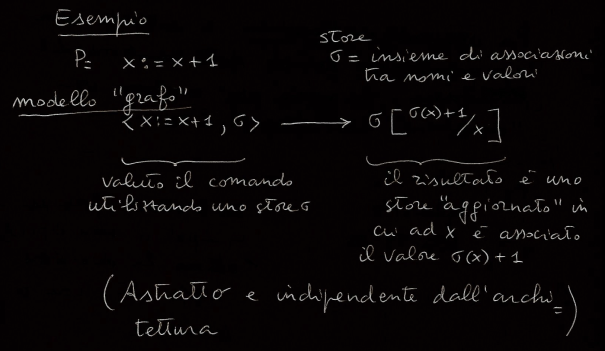
\includegraphics[width=10cm]{esempio-semantica-dinamica.png}
}

\subsection{Utilità della semantica dinamica}
A chi serve la semantica dinamica?

\begin{itemize}
    \item \textbf{Al programmatore}: \textit{ANALISI DEL PROGRAMMA}
    \begin{itemize}
        \item deve sapere esattamente cosa debba fare il suo programma
        \item deve poter dimostrare proprietà del suo programma (ad es.: "termina sempre per ogni possibile input?")
    \end{itemize}
    
    \item \textbf{Al progettista del linguaggio}:
    \begin{itemize}
        \item strumento di specifica del linguaggio
        \item deve poter dimostrare proprietà del linguaggio (ad es.: "è Turing-completo?")
    \end{itemize}
    
    \item \textbf{All'implementatore del linguaggio}:
    \begin{itemize}
        \item riferimento per dimostrare la correttezza dell'implementazione
        
        Infatti \red{un compilatore è corretto quando preserva la semantica dinamica}, quindi per dimostrare che un compilatore è corretto serve avere una semantica per il linguaggio sorgente e per il linguaggio oggetto
    \end{itemize}
\end{itemize}

\subsection{definire la semantica}
Per definire la semantica si utilizzano due tecniche principali: 
\begin{itemize}
    \item \textbf{operazionale}: (macchina astratta a stati e transizioni)
   
    Ovvero si costruisce una specie di automa che, passo a passo, mostra l'effetto dell'esecuzione delle varie istruzioni. \red{vi è una maggiore enfasi su COME si calcola}

    \item \textbf{Denotazionale}: si associa ad ogni programma sequenziale una funzione da input ad output (incluse strutture ausiliarie e memoria). \red{vi è una maggiore enfasi su COSA si calcola}
        
\end{itemize}
\section{Pragmatica nella descrizione di un linguaggio}
\dfn{Pragmatica nella descrizione di un linguaggio}{
    si definisce \textbf{pragmatica nella descrizione di un linguaggio} insieme di regole sul modo in cui è meglio usare le istruzioni a disposizione
}
Esempietti:
\esempio{
    \begin{itemize}
        \item evitare le istruzioni di salto quando possibile
        \item usare le variabili di controllo del \texttt{for}  solo a quello scopo
        \item scelta della modalità più appropriata di passaggio di paramatri ad una funzione
        \item scelta tra iterazione determinata (\texttt{for}) e indeterminata (\texttt{while})
    \end{itemize}
}
\section{
    implementazione
}
\dfn{implementazione}{
    Per \textbf{implementazione} si intende la scrittura di un compilatore per una macchina ospite già realizzata, costruendo così una macchina astratta per il linguaggio
}

\subsection{Correttezza dell'implementazione}

Per far sì che un compilatore sia corretto occorre \red{dimostrare che il programma preservi la semantica}, ovvero il programma sorgente e quello oggetto calcolino la stessa funzione 

\subsection{Struttura di un compilatore}
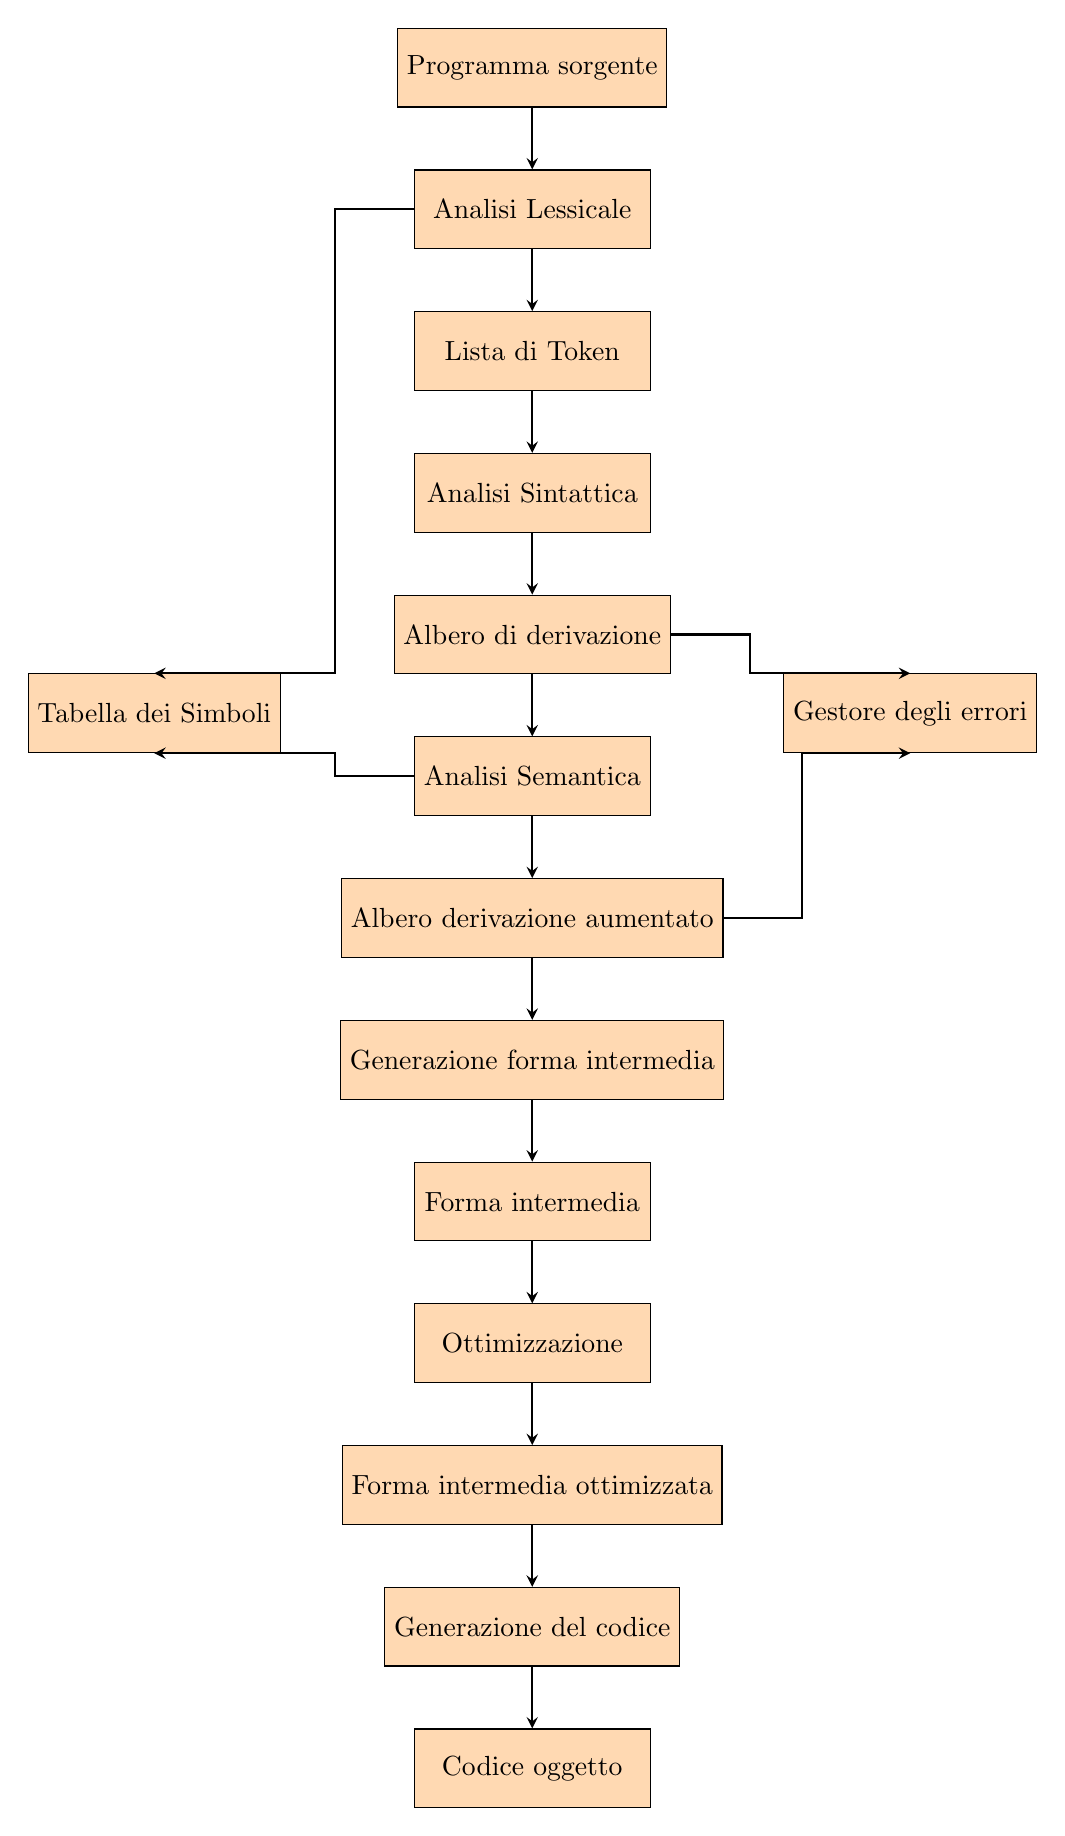
\begin{tikzpicture}[node distance=1.8cm]

    % Blocchi principali
    \node (start) [process] {Programma sorgente};
    \node (lex) [process, below of=start] {Analisi Lessicale};
    \node (tokens) [process, below of=lex] {Lista di Token};
    \node (syn) [process, below of=tokens] {Analisi Sintattica};
    \node (tree) [process, below of=syn] {Albero di derivazione};
    \node (sem) [process, below of=tree] {Analisi Semantica};
    \node (augTree) [process, below of=sem] {Albero derivazione aumentato};
    \node (interForm) [process, below of=augTree] {Generazione forma intermedia};
    \node (form) [process, below of=interForm] {Forma intermedia};
    \node (opt) [process, below of=form] {Ottimizzazione};
    \node (optForm) [process, below of=opt] {Forma intermedia ottimizzata};
    \node (codeGen) [process, below of=optForm] {Generazione del codice};
    \node (objectCode) [process, below of=codeGen] {Codice oggetto};
    
    % Frecce principali
    \draw [arrow] (start) -- (lex);
    \draw [arrow] (lex) -- (tokens);
    \draw [arrow] (tokens) -- (syn);
    \draw [arrow] (syn) -- (tree);
    \draw [arrow] (tree) -- (sem);
    \draw [arrow] (sem) -- (augTree);
    \draw [arrow] (augTree) -- (interForm);
    \draw [arrow] (interForm) -- (form);
    \draw [arrow] (form) -- (opt);
    \draw [arrow] (opt) -- (optForm);
    \draw [arrow] (optForm) -- (codeGen);
    \draw [arrow] (codeGen) -- (objectCode);
    
    % Tabelle di simboli e gestore degli errori
    \node (symTab) [process, left of=tree, xshift=-3cm, yshift=-1cm] {Tabella dei Simboli};
    \node (errManager) [process, right of=tree, xshift=3cm, yshift=-1cm] {Gestore degli errori};
    
    % Frecce verso la tabella dei simboli
    \draw [arrow] (lex.west) -- ++(-1,0) |- (symTab.north);
    \draw [arrow] (sem.west) -- ++(-1,0) |- (symTab.south);
    
    % Frecce verso il gestore degli errori
    \draw [arrow] (tree.east) -- ++(1,0) |- (errManager.north);
    \draw [arrow] (augTree.east) -- ++(1,0) |- (errManager.south);
    
\end{tikzpicture}

\section{fasi principali della compilazione}
\subsection{analisi lessicale (scanner)}
L'analisi lessicale spezza il programma sorgente nei componenti sintattici primitivi chiamati "tokens" (identificatori, numeri, operatori, parametri, parole riservate)
\begin{itemize}
    \item controlla solo che il lessico sia ammissibile 
    \item riempie parzialmente la tabello dei simboli per gli identificatori di variabili, procedure funzioni $\dots$
\end{itemize}

Per realizzare uno scanner avremo bisogno di studiare:
\begin{itemize}
    \item \textbf{grammatiche regolari}
    \item \textbf{espressioni regolari}: un formalismo usato per descrivere i linguaggi generati da grammatiche regolari 
    \item \textbf{automi a stati finiti}: uno strumento che permette di riconoscere i linguaggi regolari
\end{itemize}

\subsection{analisi sintattica (parser)}
A partire dalla lista di tokens, generata dallo scanne, il parser produce l'albero di derivazione del programma, riconoscendo se le frasi sono sintatticamente corrette

Ad esempio controlla che: 
\begin{itemize}
    \item le parentesi siano bilanciate: \texttt{((a)+b)))}
    \item che i comandi siano composti secondo le regole grammaticali \texttt{if(x=5) then then x:=3}
\end{itemize}

Per realizzare un Parser, avremo bisogno di:
\begin{itemize}
    \item grammatiche libere dal contesto
    \item automi a pila
\end{itemize}

\subsection{Analisi semantica}
l'analisi semantica \red{esegue dei controlli di semantica statica} (ovvero sintattici contestuali) per rilevare eventuali errori semantici

Arricchisce l'albero di derivazione generato dal Parser con informazioni sui tipi, verifica i tipi negli assegnamenti, parametri attuali vs. formali, dichiarazione e uso di variabili e genera eventuali errori

\subsection{Generazione della forma intermedia}
Genera codice scritto in un \textbf{linguaggio intermedio} indipendente dall'architettura, facilmente traducibile nel linguaggio macchina di varie macchine diverse. Nel generare questo codice intermedio si esegue la struttura dell'albero sintattico, ricavato dall'albero di derivazione

\subsection{Ottimizzazione}
Si effettuano ottimizzazioni nel codice intermedio per renderlo più efficiente
\begin{itemize}
    \item rimozione di codice inutile (dead code) 
    \item espansione in linea di chiamate di funzioni
    \item fattorizzazione di sottoespressioni
    \item mettere fuori dai cicli sottoespressioni che non variano
\end{itemize}

Alla fine si ottiene un codice intermedio \textbf{ottimizzato}
\subsection{Generazione del codice}
Viene generato codice per una specifica architettura (include anche l'assegnazione dei registri e ottimizzazioni specifiche macchine)

\subsection{Tabella dei simboli}
Memorizza le informazioni sui nomi presenti nel programma (identificatori di variabili, funzioni, procedure)

Es: per le matrice mette, come attributo la dimensione e il tipo dei suoi elementi 

\section{semantica operazionale strutturata}
\subsection{Definizione di un linguaggio a cui dare semantica}
lA \textbf{semantica operazionale strutturata} È utilizzata per descrivere come ogni singola istruzione o espressione in un linguaggio modifica lo stato di un sistema in termini di transizioni di stato

Il suo \textbf{linguaggio} viene \red{definito tramite sintassi atratta semplice ed intuitiva, ma ambigua} ed una stringa viene sempre accoppiata ad un albero sintattico (non ambiguo)

Alcuni elementi fondamentali del linguaggio vengono definiti attraverso \textbf{insiemi di base}:
\begin{itemize}

    \item \textbf{Booleani}: l'insieme dei valori booleani è composto da due valori: \texttt{$\{$tt,ff$\}$}. Le metavariabili sono $t,t_1,t'\in\mathbb{T}$

    \item \textbf{numeri naturali}: $\{0,1,2,\dots\} \quad n,m,p\in\mathbb{N}$
    
    \item \textbf{variabili}: ${a,b,c,\dots, z} \quad v\in Var$
\end{itemize}

Per descrivere espressioni più complesse, vengono definiti alcuni \textbf{insiemi derivati} utilizzando la notazione BNF (Backus-Naur Form)
\begin{itemize}
    \item \textbf{espressioni aritmetiche} (\texttt{exp}):
        \[
            e::= m | v | e+e|e-e|e*e    
        \]
    \item \textbf{espressioni booleane} (\texttt{Bexp}):
    \[
        b::= t|e=e|b \text{ or } b | \lnot b    
    \]
    \item \textbf{Comandi} \texttt{Com}:
    \[
        c::=\text{skip}|v:=e |c;c|\text{ while }b\text{ do }c|\text{if }b\text{ then }c\text{ else }c    
    \]
\end{itemize}

Questo tipo di sintassi è piuttosto semplice ma è ambigua, \red{per una sintassi non ambigua ne dovrei costruire una completa, ma molto più complicata} (dovrei gestire le precedenze, le parentesi ecc...) ma non serve nel dare una semantica in un linguaggio di programmazione perché un \red{parser (analizzatore sintattico) prende in input un programma scritto in sintassi concreta (non ambigua) e restituisce un albero sintattico di sintassi astratta} (quella che stiamo appena definendo), pertanto, nel dare semantica possiamo partite dagli alberi di sintassi astratta (ambigua) e ignorare la parte di anali del parser

\esempio{
    Riportiamo qui un esempio di sintassi astratta.

    Che tipo di albero sintattico vogliamo intendere con la seguente espressione? 
    \[\text{ while }b\text{ do }c_1;c_2\]
    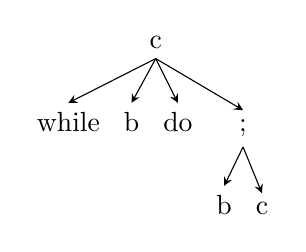
\begin{tikzpicture}
        \Tree [.c
                    [
                        .while
                    ]
                    [
                        .b
                    ] 
                    [
                        .do
                    ]
                    [
                        .; 
                        [.b ] 
                        [.c ] 
                    ] 
                ]
    \end{tikzpicture}
    %TODO LEZ10 P. 2 COMPLETARE
}

\section{Dare semantica ad un linguaggio}
Entriamo nel vivo del discorso, ma prima definiamo, per ogni categoria sintattica (cioè \texttt{Exp}, \texttt{Bexp}, \texttt{Com})un modello detto \textbf{sistema di transizione} che è fondamentalmente un "grafo" di stati

\dfn{sistema di transizione}{
    Un \textbf{sistema di transizione} è una tripla $\langle \Gamma, T, \rightarrow \rangle$ dove
    \begin{itemize}
        \item $\Gamma$ è l'insieme di stati (o configurazione)
        \item $T \subseteq \Gamma$ è l'insieme degli stati terminali (ovvero tutti quegli stati in cui il calcolo è stato terminato con successo)
        \item $\rightarrow \subseteq \Gamma\times\Gamma$ è la relazione di transazione che prende in input uno stato $\in \Gamma$ e restituisce un'altro stato $\in\Gamma$
    \end{itemize}
}
Una computazione a partire dallo stato $\gamma_0$ è una sequenza $\gamma_0\rightarrow\gamma_1\rightarrow\gamma_2\rightarrow\dots$ che può essere finita o infinita, invece con $\rightarrow^*$ si indica la chiusura riflessiva  e transitiva di $\rightarrow$, ovvero:
\[
    \frac{}{\gamma \rightarrow^* \gamma} \quad \frac{\gamma \rightarrow^* \gamma' \quad \gamma' \rightarrow \gamma''}{\gamma \rightarrow^* \gamma''}    
\]
ovvero si può raggiungere da uno stato \red{$\gamma$ uno stato $\gamma''$ in più passi}

\esempio{
    \begin{center}
    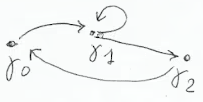
\includegraphics[width=10cm]{rappr-grafica-grafo.png}
    \end{center}
    Questa è una rappresentazione grafica di un grafo in cui i nodi sono gli stati e gli archi le transizioni
}

Se voglio definire la semantica (se voglio usare questo tipo di struttura) del linguaggio con la sintassi definita prima occorre definire uno stato di transazione specifico per \texttt{Exp}, per \texttt{Bexp} e per \texttt{Com}

Vi sono tuttavia \red{diversi problemucci}, del tipo:
\begin{enumerate}
    \item $\Gamma$ è di solito un insieme infinito contabile, allora vi è la \red{necessità di trovare una rappresentazione finita ed implicita attraverso grammatiche}. Questo vuol dire che $\Gamma$ coincide con uno dei linguaggi delle 3 categorie sintattiche (ovvero \texttt{Exp}, \texttt{Bexp}, \texttt{Com})
    \esempio{
        \[
            \Gamma_e = \{\langle e,\sigma \rangle | e \in Exp, \sigma \in Store\}
        \]
        Dove $\sigma$ è una funzione che associa ad ogni variabile un numero naturale, perché lo stato del mio sistema è una coppia in cui la prima parte indica l'espressione che devo valutare, la seconda componente è lo store che indica il valore dell'espressione   
    }
    \item $\rightarrow \subseteq \Gamma\times\Gamma$ è una relazione costituita da infinite coppie $\gamma \rightarrow \gamma'$, anche qui vi è la necessità di trovare una rappresentazione finita ed implicita come minima relazione che soddisfa \red{un certo insieme finito di assiomi e regole di inferenza}, quindi la semantica non è che un insieme di regole di inferenza che mi indicano in modo calcolare le transizioni che mi portano ad eseguire un certo comando
    \item per dare significato alle variabili (che posono solo assumere valore su $\mathbb{N}$) è necessario introdurre uno \textbf{store} $\sigma:Var\rightarrow \mathbb{N}$, come funzione che associa ad ogni variabile un valore
    \[
        \sigma = \{x_1/n_1, x_2/n_2, \dots, x_k/n_k\}    
    \]
    Se supponiamo che $var = \{x_1, x_2, \dots, x_k\}$
\end{enumerate}

\subsection{Semantica delle espressioni artimetiche}
Adesso introduciamo la \textbf{Semantica delle espressioni aritmetiche}, un tipo di semantica operazionale. Deve ovviamente avere un sistema di transizione $\langle \Gamma_e, T_e, \rightarrow_e \rangle$ dove:
\begin{itemize}
    \item $\Gamma_e = \{ \langle e, \sigma \rangle | e \in Exp, \sigma\in Store\}$
    \item $T_e = \{ \langle n, \sigma \rangle | n \in \mathbb{N}, \sigma\in Store\}$
    \item La relazione $\rightarrow_e$ è definita come la minima relazione che soddisfa gli assiomi e le regole di inferenza qui sotto:
    \begin{enumerate}
        \item \textbf{Variabile}:
        \[
        \frac{}{\langle v, \sigma \rangle \rightarrow_e \langle \sigma(v), \sigma \rangle}    
        \]
        Ovvero il tuo stato terminale sarà il numero della variabile $v$ indicato dallo Store (inoltre $\sigma$ rimane inalterato). Quindi valuto ciò che $v$ vale in $\sigma$
        \item \textbf{Somma 1}:
        \[
            \frac{\langle e_0, \sigma \rangle \rightarrow_e \langle e_0', \sigma' \rangle}{\langle e_0 + e_1, \sigma \rangle \rightarrow_e \langle e_0' + e_1, \sigma' \rangle}
        \]

        Nel momento in cui riesco a fare un passo di valutazione da $e_0$ a $e_0'$ alterando anche lo stato dello store da $\sigma$ a $\sigma'$ questa trasformazione si anche applicare durante una somma, in altre parole l’espressione si semplifica o riduce (ad esempio, una variabile viene sostituita con il suo valore), e nel contempo lo stato della memoria potrebbe essere aggiornato se l’espressione stessa comporta una modifica ai valori delle variabili

        \item \textbf{Somma 2}:
        \[
            \frac{\langle e_1, \sigma \rangle \rightarrow_e \langle e_1', \sigma' \rangle}{\langle m + e_1, \sigma \rangle \rightarrow_e \langle m + e_1', \sigma' \rangle}
        \]
        Stessa roba ma con un numero $m$
        \item \textbf{Somma 3}:
        \[
            \frac{}{\langle m+m', \sigma \rangle \rightarrow_e \langle P, \sigma \rangle}   \quad \text{ dove } P = m+m' 
        \]
        \item \textbf{Sottrazione 1}:
        \[
            \frac{\langle e_0, \sigma \rangle \rightarrow_e \langle e_0', \sigma' \rangle}{\langle e_0 - e_1, \sigma \rangle \rightarrow_e \langle e_0' - e_1, \sigma' \rangle}
        \]
        \item \textbf{Sottrazione 2}:
        \[
            \frac{\langle e_1, \sigma \rangle \rightarrow_e \langle e_1', \sigma' \rangle}{\langle m - e_1, \sigma \rangle \rightarrow_e \langle m - e_1', \sigma' \rangle}
        \]
        \item \textbf{Sottrazione 3}:
        \[
            \frac{}{\langle m - m', \sigma \rangle \rightarrow_e \langle p, \sigma \rangle}
        \]
        
   

    \end{enumerate}

    Si noti come la somma e la sottrazione prima valutano la sottoespressione di sinistra ($e_0$) con somma/sottrazione 1 poi, se questa s'è mutata in numero, valutano la sottoespressione di destra ($e_1$) con somma/sottrazione 2 ed infine, se questa s'è mutata in un numero, viene fatta la somma/sottrazione finale con somma/sottrazione 3

    \esempio{
        Esempietto per valutare $\langle (x+2)-y, \{x/5, y/3\} \rangle$:
        
        \begin{center}
            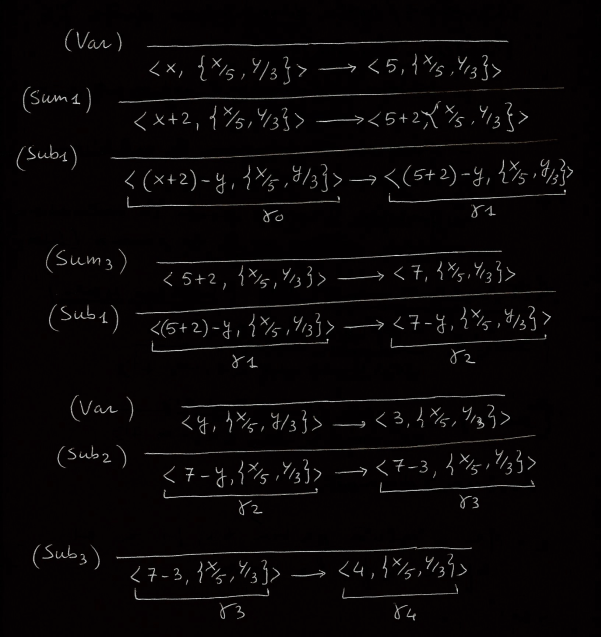
\includegraphics[width=10cm]{esempio-di-transizione.png}
        \end{center}

        Si ha, quindi, che $\gamma_0\rightarrow\gamma_1\rightarrow\gamma_2\rightarrow\gamma_3\rightarrow\gamma_4\in T_e$ cioè $\langle (x+2)-y, \{x/5, y/3\} \rangle \rightarrow^*\langle 4, \{x/5, y/3\} \rangle$
    }
\end{itemize}

\teorema{
    Vogliamo dimostrare che $\rightarrow_e$ è deterministico, ovvero:
    \[
        \gamma\rightarrow_e\gamma'\text{ e } \gamma\rightarrow_e\gamma''\text{, allora }\gamma'=\gamma''\quad \forall \gamma,\gamma',\gamma''  
    \]

    In altre parole significa che \red{da ogni transizione esce al più una transizione}, mai più di una
}
\pf{dimostrazione}{
    mi riduco a dimostrare che $(\inside{e,\sigma}\rightarrow_e \gamma' \land \inside{e,\sigma}\rightarrow_e\gamma'')\Rightarrow\gamma'=\gamma''$ 

    Procedo per induzione strutturale, con HP $(\inside{e,\sigma}\rightarrow_e \gamma' \land \inside{e,\sigma}\rightarrow_e\gamma'')\Rightarrow\gamma'=\gamma''$.
    \begin{enumerate}
        \item $e=m\in \mathbb{N}$: se $\inside{e,\sigma}\nrightarrow_e e$ allora la conclusione è vera perché la premessa è falsa
        \item $e=v\in Var$: Per la regola (Var), l'unica transizione derivabile per $\inside{v,\sigma}$ è $\inside{v,\sigma}\rightarrow_e \inside{\sigma(v), \sigma}$ poiché $\sigma$ è una funzione (cioè $\sigma(v)$ è univoco) e la sola regola (Var) è applicabile allora per forza $\inside{\sigma(v), \sigma} = \sigma'$ e $\inside{\sigma(v), \sigma}=\sigma''$ quindi $\gamma'=\gamma''$
        \item $e = e_0 + e_1$:
            Supponiamo che $\inside{e_0+e_1,\sigma}\rightarrow\gamma'$ e $\inside{e_0+e_1,\sigma}\rightarrow\gamma''$
            
            Ci sono 3 sottocasi da esaminare in accordo nel modo in cui derivo  $\inside{e_0+e_1,\sigma}\rightarrow\gamma'$:
            \begin{enumerate}
                \item  $\inside{e_0,\sigma}\rightarrow\inside{e_0',\sigma'}$ e $\gamma'=\inside{e_0' + e_1, \sigma'}$
                in questo caso ho che $e_0 \notin \mathbb{N}$ e la regola che ho applicato è \texttt{Somma 1}. 
                Allora se $\inside{e_0+e_1, \sigma}\rightarrow \gamma''$ è necessario che $\inside{e_0, \sigma}\rightarrow \inside{e_0'', \sigma''}$ e che $\gamma''=\inside{e_0''+e_1, \sigma''}$.

                Tuttavia per (HP) si ha che $\inside{e_0',\sigma'} = \inside{e_0'',\sigma''}$ pertanto deve essere che $e_0' = e_0''$ e $\sigma' = \sigma''$, da cui discende $\gamma' = \gamma''$
                \item $e_0 = m \in \mathbb{N}$ ed $\inside{e_1, \sigma}\rightarrow\inside{e_1', \sigma'}$ 
                Caso analogo al precedente, dato che ho che $e_1\notin\mathbb{N}$ e la regola che ho applicato è \texttt{Somma 2}. Allora se $\inside{e_0 + e_1, \sigma}\rightarrow \gamma''$, è necessario che $\inside{e_1, \sigma}\rightarrow \inside{e_1'',\sigma''}$ e $\gamma'' = \inside{e_0+e_1'',\sigma''}$. Tuttavia per (HP) si ha che $\inside{e_1',\sigma'} = \inside{e_1'',\sigma''}$ pertanto deve essere che $e_1' = e_1''$ e $\sigma' = \sigma''$, da cui discende $\gamma' = \gamma''$
                \item $e_0 \in \mathbb{N}$ ed $e_1\in \mathbb{N}$
                In questo caso, solo \texttt{Somma 3} è applicabile, ottenendo una sola passibile transizione:
                \[
                    \inside{e_0+e_1,\sigma} \to\inside{P, \sigma} \text{ dove } P = e_0+e_1
                \] 
                Quindi la tesi segue:
                \[
                    \inside{e_0+e_1,\sigma}\to\gamma'\land \inside{e_0+e_1,\sigma}\to\gamma''\implies\gamma'=\gamma''
                \]
            \end{enumerate}

            \item $e=e_1-e_2$: DEL TUTTO ANALOGO AL CASO PRECEDETE
            

            
        
    \end{enumerate}
    Q.e.d.
}

Questo teorema ci porta ad un dio boia di corollario:

\cor{}{
        poiché $\to_e$ è determinisca, a partire da $\inside{e,\sigma}$ arriveremo su una sola configurazione terminale $\inside{n,\sigma}$: "n è il valore di $e$ in $\sigma$"

        È possibile perciò definire una funzione 
        \[
            eval : Expr\times Store \dashrightarrow  \mathbb{N} 
        \]
        che da semantica alle espressione
        \[
            eval (e, \sigma) = \begin{cases}
                m & \text{ se }\inside{e,\sigma}\to^* \inside{m,\sigma}  \\
                \text{indefinita} & \text{altrimenti}
            \end{cases}   
        \]
}

Esempi:
\esempio{
    \begin{itemize}
        \item $eval((x+2)- y, \{x/5, y/3\}) = 4$ dato che
        \[
            \inside{(x+2)-y, \{x/5, y/3\}} \to^* \inside{4, \{x/5, y/3\}}    
        \]
        \item $eval((x+2)-y, \{x/2, y/7\})=indefinito$ dato che
        \[
            \inside{(x+2)-y, \{x/2, y/7\}} \to^* \inside{4-7, \{x/2, y/7\}} \nrightarrow     
        \]
    \end{itemize}
}

Inoltre sia introdotta la definizione di equivalenza:
\dfn{Equivalenza tra espressioni}{
    Siano $e$ ed $e'$ due espressioni, allora si dicono \textbf{equivalenti} sse $\forall\sigma\in Store \quad eval(e,\sigma)=eval(e',\sigma)$

    E si denota con $e \equiv e'$
}
Esempietto:
\esempio{
    $v_1+(v_2+v_3)\equiv(v_1 + v_2) + v_3$
}

Si osservi come \texttt{Eval} è definita rispetto alla disciplina di valutazione \texttt{IS} (interno destro), pertanto, rigorosamente, \texttt{Eval} è denotato come $Eval_{is}$. Si può, inoltre, dimostrare che anche per \texttt{ID} (interno destro), il risultato della valutazione è lo stesso:
\[
    Eval_{is} = Eval_{id}    
\]

Dove $Eval_{id}(e,\sigma) = \begin{cases} m & \text{ se }\inside{e,\sigma}\to^*_{id} \inside{m,\sigma}  \\ \text{indefinita} & \text{altrimenti}\end{cases}$

Come vedremo, è possibile definire anche altre siscipline di valutazione come Esterna Sinistra, Esterne Destra, Esterna parallela.
\subsection{Semantica delle espressioni booleane}
Arriviamo alle espressioni booleane con la seguente grammatica:
\[
    b ::= t|e=e|b\text{ or }b| \lnot b    
\]
(ricordo che $t$ è una metavariabile con un valore di verità true o false)
E il seguente sistema di transazione:
\[
    \inside{\Gamma_b, T_b, \to_b} \text{ dove } \Gamma_b = \{\inside{b,\sigma}|b\in Bexp, \sigma\in Store\} \text{ e } T_b=\{\inside{tt,\sigma}, \inside{ff,\sigma}| \sigma\in Store\}    
\]

e $\to_b$ è la minima relazione generata dai seguenti assiomi e regole di inferenza:
\begin{itemize}
    \item \textbf{Eq1} 

    \[
        \frac{\langle e_0 = e_1, \sigma \rangle \to_b \langle e_1', \sigma' \rangle}{\langle m = e_1, \sigma \rangle \to_b \langle m = e_1', \sigma' \rangle}
    \]
    \item \textbf{Eq2}
    \[
        \frac{\inside{e_1, \sigma}\to_e\inside{e_1',\sigma'}}{\langle m = e_1, \sigma \rangle \to_b \langle m = e_1', \sigma' \rangle}
    \]
    \item \textbf{Eq3}
    \[  
        \frac{}
        {\langle m = m, \sigma \rangle \to_b \langle t, \sigma \rangle} \text{ dove } t = \begin{cases} 
            \text{tt} & \text{se } m = n \\
            \text{ff} & \text{se } m \neq n 
        \end{cases}  
    \]
    \item \textbf{Or1}
    \[
        \frac{\inside{b_0,\sigma}\to_b\inside{b_0',\sigma'}}{\inside{b_0 \text{ or }b_1,\sigma} \to_b \inside{b_0' \text{ or }b_1, \sigma'}}  
    \]
    \item \textbf{Or2}
    \[
        \frac{}{\inside{tt \text{ or }b_1, \sigma}\to_b\inside{tt, \sigma}}    
    \]
    \item \textbf{Or3}
    \[
        \frac{}{\inside{ff \text{ or } b_1, \sigma}\to_b \inside{b_1,\sigma}}    
    \]
    \item \textbf{Neg1}
    \[
        \frac{\inside{b,\sigma}\to_b\inside{b', \sigma'}}{\inside{\lnot b, \sigma}\to_b\inside{\lnot b', \sigma'}}    
    \]
    \item \textbf{Neg2}
    \[
        \frac{}{\inside{\lnot b, \sigma}\to_b\inside{t', \sigma}}\text{ dove }t' = \begin{cases}
            tt \text{ se }t=ff
            ff \text{ se }t=tt
        \end{cases}  
    \]
\end{itemize}

Si tenga presente che \texttt{Eq1}, \texttt{Eq2} e \texttt{Eq3} sono cosiddette \textbf{interne sinistre} perché inizio a valutare la sottoespressione di sinistra per poi restituire un valore di verità $t$ sse ho ottenuto numeri in tutte e due le sottoespressioni mentre  \texttt{Or1}, \texttt{Or2} e \texttt{Or3} sono \textbf{esterne sinistre} perché inizio a valutare la sottoespressione di sinistra per poi restituire un valore di verità $t$ sse ho ottenuto numeri almeno in una sottoespressione. Quindi se nelle interne dovevo avere dei numeri in tutte le sottoespressioni per poi eseguire la valutazione finale nelle esterne per eseguire la valutazione finale mi basta avere una quantità sufficiente

Anche per i booleani si ha questo teorema:
\teorema{
    $\to_b$ è deterministica, ovvero 
    \[
        (\gamma \to_b \gamma' \land \gamma\to_b\gamma'')\implies \gamma' = \gamma''    
    \]
}
Che porta al seguente corollario:
\cor{}{
    si può, quindi, definire:
    \[
        eval_b(b,\sigma) = \begin{cases}
            t & \text{se }\inside{b,\sigma}\to^*\inside{t,\sigma}\\
            \text{indefinita} & \text{altrimenti}
        \end{cases}       
    \]
}

E si ha anche la seguente definizione:
\dfn{Equivalenza booleani}{
    Siano $b$ ed $b'$ due booleani, allora si dicono \textbf{equivalenti} sse $\forall\sigma\in Store \quad eval_b(b,\sigma)=eval_b(b',\sigma)$

    E si denota con $b \equiv b'$
}
\esempio{
    \[
        \lnot((3=v)\lor (3=4)) = \lnot(v=3)       
    \]
}

Si possono definire per $b_0$ or $b_1$ regole di valutazioni diverse da \texttt{ES}. Ad esempio \texttt{ED} o \texttt{IS}, ma non sono tutte equivalenti, si provi, ad esempio, con \texttt{ED}:

\begin{itemize}
    \item \textbf{Or1'}:
    \[\frac{\inside{b_1, \sigma}\to_b\inside{b_1',\sigma'}}{\inside{b_0 \text{ or }b_1, \sigma}\to_b\inside{b_0 \text{ or } b_1', \sigma'}}\]
    \item \textbf{Or2'}:
    \[
        \frac{}{\inside{b_0 \text{ or }tt, \sigma}\to_b \inside{tt, \sigma}}    
    \]
    \item \textbf{Or3'}:
    \[
        \frac{}{\inside{b_0 \text{ or }ff, \sigma}\to_b \inside{b_0, \sigma}}    
    \]
\end{itemize}
\esempio{
    $\gamma=\inside{}$
}
  

\chapter{Analisi lessicale: espressioni regolari, DFA, NFA}
\section{analisi lessicale}
partiamo dalla definizione
\dfn{Analisi lessicale}{
    Riconoscere nella stringa in ingresso gruppi/sequenze di simboli che corrispondono a specifiche categorie sintattiche
}

La stringa in input,poi, è trasformata in una sequenza di simboli astratti, detti \textbf{token}, si analizzi la figura:
\begin{center}
    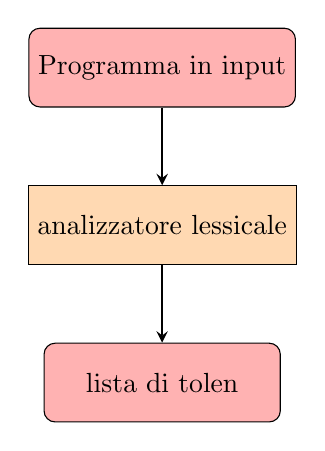
\begin{tikzpicture}[node distance=2cm]

        % Nodes
        \node (inizio) [startstop] {Programma in input};
        \node (algorithm) [process, below of=inizio] {analizzatore lessicale};
        \node (fin) [startstop, below of=algorithm] {lista di tolen};
        
        % Arrows
        \draw [arrow] (inizio) -- (algorithm);
        \draw [arrow] (algorithm) -- (fin);
        
\end{tikzpicture}
\end{center}

\subsection{token}
\dfn{Token}{
    un token è una coppia (nome, valore), dove:
    \begin{itemize}
        \item il \textit{nome} è un simbolo astratto che rappresenta una categoria semantica
        \item il \textit{valore} una sequenza di simboli del testo in ingresso
    \end{itemize}
}
Esempietto:
\esempio{
    Un esempio di token è $\inside{Ide, x1}$, dove:
    \begin{itemize}
        \item $Ide$: è l'informazione che identifica una classe di token
        \item $x_1$: è l'informazione che identifica lo specifico token 
        \item 
    \end{itemize}
}
Siano inoltre tali definizioni
\dfn{Pattern}{
    è la descrizione generale della forma dei valori di una classe di token
}
\esempio{
    Sia $(x\mid y)(x\mid y\mid 0\mid 1)^*$ un'espressione regolare per rappresentare un Pattern
}

\dfn{
    lessema
}{
    si definisce \textbf{lessema} una stringa istanza di un pattern
}
\esempio{
    nel nostro esempio $x1$ è un'istanza di un pattern
}

vedremo che ad ogni nome di categoria sintattica è associato un pattern che specifica i possibili valori che possono essere presi per quel nome, come lessemi

\esempio{
    dalla strinfa $C$ si ha:
    \begin{center}
        \texttt{if}$(x==0)$ \texttt{printf("zero")}
    \end{center}

    un analizzatore lessicale potrebbe produrre la seguente sequenza di token:
    \begin{itemize}
        \item $\inside{\text{\texttt{if}}}$
        \item $\inside{\text{\texttt{(}}}$
        \item $\inside{ide, x}$
        \item $\inside{Operel, ==}$
        \item $\inside{const-num, 0}$
        \item $\inside{\text{\texttt{)}}}$
        \item $\inside{Ide, \text{\texttt{printf}}}$
        \item $\inside{\text{\texttt{(}}}$
        \item $\inside{const-string, \text{\texttt{zero}}}$
        \item $\inside{\text{\texttt{)}}}$
    \end{itemize}
}
In realtà, normalmente lo scanner \red{associa agli identificatori un indirizzo della tabella dei simboli}, quindi  $\inside{ide, x}$ è in realta  $\inside{ide, \text{puntatore alla tabello dei simboli}}$

\subsection{espressioni regolari}
Nello stesso modo in cui possiamo scrivere espressioni matematiche utilizzando operatori matematici ($ +, \times,... $) e' possibile, utilizzando appositi operatori regolari, definire \textbf{espressioni regolari} che descrivono un linguaggio. Ad esempio:
\[
  (a \mid b)c^*
\]
dove 'a', 'b' e 'c' vengono intesi come i linguaggi $ \{a\} $, $ \{b\} $ e $ \{c\} $, '$ \mid $' e' l'operazione di unione, quindi $ \{a\} \cup \{b\} = \{a, b\} $. Fra le parentesi e la 'c' e' sottintesa l'operazione di congiunzione '$ \cdot $', ma ha priorita' l'operatore $ ^* $ che ha lo stesso effetto della stella di Kleene. Quindi diventa:
\[
  \{a, b\}\cdot \{c\}^* = \{a, b, ac, bc, acc, bcc, ...\}
\]
Definiamo formalmente questo tipo di espressioni e i linguaggi che definiscono:
\dfn{espressioni regolari}{
    fissato un alfabeto $A =\{a_1,a_2,\dots,a_n\}$, definiamo le espressioni regolari su $A$ con la seguente $BNF$
    \[
        r::= \varnothing\mid\varepsilon\mid a\mid r\cdot r\mid r|r\mid r^*    
    \]
}
\nt{
  La definizione non e' ciclica perche' le espressioni sono definite da altre espressioni piu' piccole.
}
\nt{
  Non confondere le ER $ \emptyset $ e $ \varepsilon $: la prima identifica il linguaggio vuoto, che non accetta nessuna stringa, mentre il linguaggio associato alla seconda accetta la stringa vuota.
}
\nt{
    Si tenga presente che questa è una sintassi astratta ambigua, ci vorrebbero le parentesi per disanbiguare, tuttavia noi assumiamo che:
    \begin{itemize}
        \item la concatenazione, disgiunzione e ripetizione associano a \texttt{sx}
        \item la precedenza tra gli operatori sia: \texttt{* > $\cdot$ > |}
        \item la concatenazione $\cdot$ è di solito omessa
    \end{itemize}

    Per cui, ad esempio, $b*a|c$ corrisponde all'albero sintattico:
    \begin{center}
        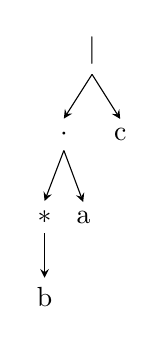
\begin{tikzpicture}
            \Tree[
                .$|$
                [
                    .$\cdot$
                    [
                        .$*$
                        b
                    ]
                    a
                ]
                c
            ]
        \end{tikzpicture}
    \end{center}
    
    Quindi secondo una sintassi non ambigua: $(((b)^*)\cdot(a))|(c)$ 
}
\subsubsection{linguaggio denotato da una espressione regolare}
\dfn{}{
    dato l'alfabeto $A$, definiamo la funzione:
    \[
        \mathcal{L}:\text{\texttt{Exp-Reg}}\to\mathcal{P}(A^*)
    \]
    Come segue:
    \begin{align*}
        \mathcal{L}[\varnothing] &= \varnothing \text{ (linguaggio vuoto)} \\
        \mathcal{L}[\varepsilon] &= \{\varepsilon\}  \text{ (linguaggio che contiene solo la stringa vuota)} \\
        \mathcal{L}[a] &= \{a\} \\
        \mathcal{L}[r_1 \cdot r_2] &= \mathcal{L}[r_1] \cdot \mathcal{L}[r_2] \\
        \mathcal{L}[r_1 | r_2] &= \mathcal{L}[r_1] \cup \mathcal{L}[r_2] \\
        \mathcal{L}[r^*] &= (\mathcal{L}[r])^*
    \end{align*}    
}

\nt{
    Si ricordi che:

    \begin{align*}
        L_1 \cdot L_2 &= \{xy \mid x \in L_1, y \in L_2\} \\
        L_1 \cup L_2 &= \{x \mid x \in L_1 \text{ or } x \in L_2\} \\
        L^\circ &= \{\varepsilon\} \\
        L^{n+1} &= L \cdot L^n \\
        L^* &= \bigcup_{n \geq 0} L^n
    \end{align*}
    
}
\subsubsection{linguaggio regolare}
\dfn{Linguaggio regolare}{
    un linguaggio $L\subseteq A^*$ è definito regolare sse $\exists$ una espressione regolare $r$ tale che:
    \[
        L=\mathcal{L}[r]    
    \]
    
}
\mprop{}{
     ogni linguaggio finito è regolare   
    }
\esempio{
    Sia $L=\{a,bc\}$ con $r=a\mid bc$
    si ha che:
    \[
            \mathcal{L}[a\mid bc] = \mathcal{L}[a]\cup \mathcal{L}[bc] =\{a\}\cup \mathcal{L}[b]\cdot \mathcal{L}[c] = \{a\}\cup\{b\}\cdot\{c\} = \{a,bc\}=L
    \]
}

Si osservi che esistono anche linguaggi regolari infiniti:
\[
\begin{aligned}
    \mathcal{L}[a^*b] &= \mathcal{L}[a^*] \cdot \mathcal{L}[b] = (\mathcal{L}[a])^* \cdot \mathcal{L}[b] \\
    &= \{a\}^* \cdot \{b\} = \bigcup_{m \geq 0} \{a^m\} \cdot \{b\} \\
    &= \{\varepsilon, a, aa, \ldots\} \cdot \{b\} = \{a^m b \mid n \geq 0\}.
\end{aligned}
\]

\[
\begin{aligned}
    \mathcal{L}[a \mid a^*b] &= \mathcal{L}[a] \cup \mathcal{L}[a^*b] = \{a\} \cup \{a^m b \mid n \geq 0\}.
\end{aligned}
\]

\[
\begin{aligned}
    \mathcal{L}[(a \mid b) \cdot b^*] &= \mathcal{L}[a \mid b] \cdot \mathcal{L}[b^*] = (\mathcal{L}[a] \cup \mathcal{L}[b]) \cdot (\mathcal{L}[b])^* \\
    &= \{a, b\} \cdot \{b\}^* = \{a b^m \mid n \geq 0\} \cup \{b^n \mid n \geq 1\}.
\end{aligned}
\]

\ex{espressioni regolari}{
    $A=\{0,1\}$
    \begin{itemize}
        \item $0^*10^*$
        
        Con $\quad L_2\{w\in A^*\mid A^*\mid w \text{ contiene un solo }1\}$
        \item $(0\mid 1)^*001(0\mid1)^*$
        
        Con $\quad L_1\{w\in A^*\mid A^*\mid w \text{ contiene un solo }1\}$
        \item $1^*(011^*)^*$
        
        Con $\quad L_3 =\{w\in A^*\mid w \text{ contiene }001 \text{ come sottostringa}\}$
    \end{itemize}
}
\subsubsection{altri operatori ausiliari}
% TODO non ho voglia, ma io si
\dfn{}{
  \begin{itemize}
    \item Ripetizione positiva: $ r^+ = rr* $
    \item Possibilita': $ r? = r \mid \varepsilon $
    \item Elenco: $ [a_1, ..., a_n] = a_1 \mid ... \mid a_n $
  \end{itemize}
}

\subsection{equivalenza tra espressioni regolari}
\dfn{
    equivalenza
}{
    Due espressioni regolari $r$ ed $s$ sono \textbf{equivalenti} sse $\mathcal{L}[r]=\mathcal{L}[s]$ (cioè demotano lo stesso linguaggio) e lo denotiamo con $r\equiv s$
}

Esistono molte leggi per $\equiv$, alcune sono le seguenti 
\begin{align*}
    r | s &\equiv s | r \quad \text{(1 è commutativa)} \\
    r | (s | t) &\equiv (r | s) | t \quad \text{(1 è associativa)} \\
    z | z &\equiv z \quad \text{(1 è idempotente)} \\
    z \cdot (s \cdot t) &\equiv (z \cdot s) \cdot t \quad \text{($\cdot$ è associativa)} \\
    \varepsilon \cdot z &\equiv z \cdot \varepsilon \equiv z \quad \text{($\varepsilon$ è l'elemento neutro per $\cdot$)} \\
    (r^*)^* &\equiv r^* \quad \text{(* è idempotente)} \\
    r (s | t) &\equiv r s | r t \quad \text{(distribuisce a sinistra su |)} \\
    (r | s) t &\equiv r t | s t \quad \text{(distribuisce a destra su |)}
\end{align*}

In alcuni casi è facile dimostrare queste leggi:
\begin{align*}
    \mathcal{L}[r | s] &= \mathcal{L}[r] \cup \mathcal{L}[s] \\
    &= \mathcal{L}[s] \cup \mathcal{L}[r] \\
    &= \mathcal{L}[s | r] \\
    \\
    \mathcal{L}[r | r] &= \mathcal{L}[r] \cup \mathcal{L}[r] \\
    &= \mathcal{L}[r] \\
    \\
    \mathcal{L}[r \varepsilon] &= \mathcal{L}[r] \cdot \{\varepsilon\} \\
    &= \mathcal{L}[r] \\
    \\
    \mathcal{L}[\varnothing^*] &= (\mathcal{L}[\varnothing])^* \\
    &= \varnothing^* \\
    &= \varnothing^0 \cup \varnothing^1 \cup \varnothing^2 \cup \dotsb \\
    &= \{\varepsilon\} \cup \varnothing \cup \varnothing \\
    &= \{\varepsilon\} \\
    &= \mathcal{L}[\varepsilon] \\
    \\
    \mathcal{L}[r \cdot \varnothing] &= \mathcal{L}[r] \cdot \mathcal{L}[\varnothing] \\
    &= \mathcal{L}[r] \cdot \varnothing \\
    &= \varnothing \\
    &= \mathcal{L}[\varnothing]
\end{align*}


Le espressioni regolari servono per specificare il pattern di una categoria sintattica, ovvero la forma dei possibili lessemi, tuttavia occorre riconoscere se una certa sequenza in ingresso è un lessema per una certa categoria sintattica. A questo ci vengono in aiuto gli automi a stati finiti

\section{Automi a stati finiti}
Un \textbf{automa a stati finiti} (o DFA, deterministic finite automaton, per la versione deterministica) è un modello computazionale utilizzato per rappresentare e analizzare linguaggi regolari. È un \red{dispositivo astratto che processa stringhe di simboli e decide se appartengono o meno a un linguaggio}

Si può immaginare il DFA come una automa ideale dotato di una testina di lettura, una sequenza di simboli in input da leggere e un sistema di stati, del tipo

%todo aggiungere immagine 

Dove inizialmente 
\begin{itemize}
    \item la testina di lettura è posizionata sul primo carattere dell'input
    \item e vi è un controllo su sullo stato iniziale $q_0$
\end{itemize}

E funziona ciclicamente nel modo seguente:
\begin{itemize}
    \item leggi il carattere in input e in baso allo stato in cui si trova decide:
    \begin{itemize}
        \item di cambiare di stato
        \item di spostare la testina sull'input successivo
    \end{itemize}
    FINO A CHE:
    \item ha finito di leggere l'input (e riconosce la stringa)
    \item non ha riconosciuto la stringa 
\end{itemize}

\subsection{diagrammi di transazione}
il funzionamento di un automa finito  è ben descritto dai cosiddetti \textbf{diagrammi di transizione}

\begin{center}
    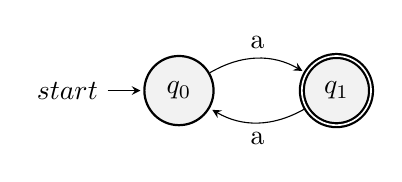
\begin{tikzpicture}[shorten >=1pt, node distance=2cm, on grid, auto] 
    \node[state, initial] (q_0)   {$q_0$}; 
    \node[state, accepting] (q_1) [right=of q_0] {$q_1$}; 
     
    \path[->] 
     (q_0) edge [bend left] node {a} (q_1)
     (q_1) edge [bend left] node {a} (q_0);
 \end{tikzpicture}
\end{center}

Riconoscere una stringa $w$ significa trovare un cammino etichettato $w$ sul grafo a partire dallo stato iniziale che finisce su uno stato finale 
\[
    L =\{a^{2n+1}\mid n\geq 0\} = \{a^n\mid n \text{ è dispari}\} = \mathcal{L}[a(aa)^*]    
\]
\esempio{
    \begin{itemize}
        \item Primo esempio:
        Sia $L=\{w\in \{0,1\}^*\mid \text{ in  }w\text{ il numero di }0\text{ e }1\text{ è sempre pari}\}$

        Il suo automa è:
        \begin{center}
            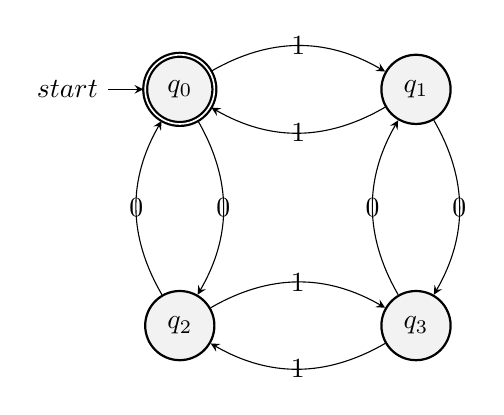
\begin{tikzpicture}
            \node[state, initial, accepting] (q0) {$q_0$};
            \node[state, right of=q0] (q1) {$q_1$};
            \node[state, below of=q0] (q2) {$q_2$};
            \node[state, right of=q2] (q3) {$q_3$};
            
            \path[->]
            (q0) edge [bend left] node {$1$} (q1)
            (q1) edge [bend left] node {$1$} (q0)

            (q2) edge [bend left] node {$1$} (q3)
            (q3) edge [bend left] node {$1$} (q2)

            (q2) edge [bend left] node {$0$} (q0)
            (q0) edge [bend left] node {$0$} (q2)

            (q1) edge [bend left] node {$0$} (q3)
            (q3) edge [bend left] node {$0$} (q1);
            
        \end{tikzpicture}
        \end{center}
        \item secondo esempio
        
        Sia $L=\mathcal{L}[(a|b)^*ba]$

        il suo automa è:
        \begin{center}
            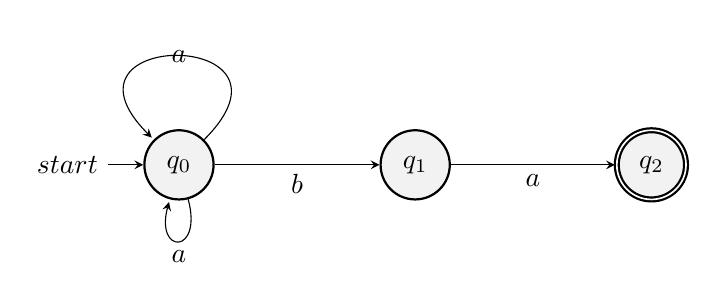
\begin{tikzpicture}
                \node[state, initial] (q0) {$q_0$};
                \node[state, right of=q0] (q1) {$q_1$};
                \node[state, accepting, right of=q1] (q2) {$q_2$};

                \path[->]
                    (q0) edge[loop below] node {$a$} (q0)
                    (q0) edge[loop ] node {$a$} (q0)
                    (q0) edge[below] node {$b$} (q1)
                    (q1) edge[below] node {$a$} (q2);
            \end{tikzpicture}
        \end{center}

        Si noti che $ba\in L[M]$ (ovvero $ba$ appartiene al linguaggio riconosciuto dall'automa $M$)  perché esiste un cammino da $q_0$ a $q_2$ etichettato $ba$

        Questo linguaggio è \red{non deterministico}:
        \begin{itemize}
            \item $(q_0, b)$ offre 2 mosse o su $q_0$ o su $q_1$
            \item $(q_1, b)$ non offre mosse
            \item $(q_2, a/b)$ non offre mosse 
        \end{itemize}

        \item terzo esempio:
        
        Sia $L[M]=\mathcal{L}[a^*b^*]$

        Riconosciuto dal seguente automa:
        \begin{center}
            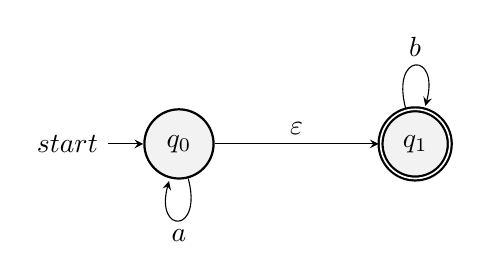
\begin{tikzpicture}
                \node[state, initial] (q0) {$q_0$};
                \node[state, accepting, right of=q0] (q1) {$q_1$};

                \path[->]
                    (q0) edge[loop below] node {$a$} (q0)
                    (q0) edge[above] node {$\varepsilon$} (q1)
                    (q1) edge[loop above] node {$b$} (q1);
            \end{tikzpicture}
        \end{center}

        Che \red{nondeterministico} perché è possibile spostarsi dallo stato $q_0$ allo stato $q_1$ senza leggere l'input. 
        
        Se vogliamo un automa deterministico:
        \begin{center}
            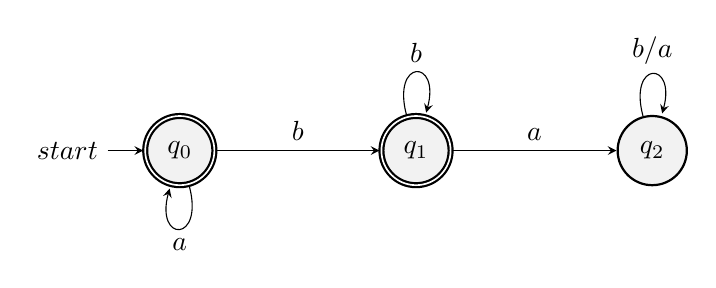
\begin{tikzpicture}
                \node[state, accepting, initial] (q0) {$q_0$};
                \node[state, accepting, right of=q0] (q1) {$q_1$};
                \node[state, right of=q1] (q2) {$q_2$};

                \path[->]
                    (q0) edge[loop below] node {$a$} (q0)
                    (q0) edge[above] node {$b$} (q1)
                    (q1) edge[loop above] node {$b$} (q1)
                    (q1) edge[above] node {$a$} (q2)
                    (q2) edge[loop above] node {$b/a$} (q2);
            \end{tikzpicture}
        \end{center}   
        Dove $q_2$ è uno stato pozzo d'errore. Inoltre da ogni stato per ognuno dei due simboli ($a$ e $b$), esce una e una sola transizione e non vi sono transizioni $\varepsilon$

        
    \end{itemize}
}
\subsection{Automi a stati finiti non deterministico}
Adesso formalizziamo la definizione
\dfn{Automi a stati finiti non deterministici}{
    Si defisnisce  \textbf{NFA o automa a stati finiti non deterministico} una quintupla $(\Sigma, Q, \delta, q_0, F)$ dove:
    \begin{itemize}
        \item $\Sigma$ è un alfabeto finito di simboli in input
        \item $Q$ è un insieme finito di stati
        \item $q_0\in Q$ è lo stato iniziale 
        \item $F\subseteq Q$ è l'insieme degli stati finali
        \item $\delta$ è la funzione di transizione con tipo
        
        \[
            \delta : Q\times (\Sigma\cup\{\varepsilon\})\to \mathcal{P}(q)    
        \]
    \end{itemize}
    
}
Esempietto:
\esempio{
    \[
        \Sigma = \{a, b\} \quad Q = \{q_0, q_1, q_2\} \quad q_0 \text{ iniziale} \quad F = \{q_2\}
    \]

    \[
        \delta =
        \begin{array}{c|c|c|c}
            & a & b & \varepsilon \\
            \hline
            q_0 & \{q_0\} & \{q_0, q_1\} & \varnothing \\
            q_1 & \{q_2\} & \varnothing & \varnothing \\
            q_2 & \varnothing & \varnothing & \varnothing \\
        \end{array}
    \]

    \vspace{1cm}

    Si può vedere la seguente tabella mutarsi in automa
    \vspace{0.5cm}

    \begin{center}
        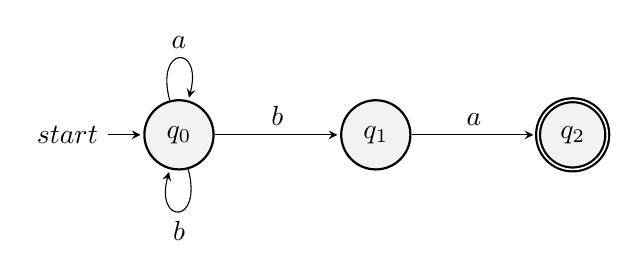
\begin{tikzpicture}[shorten >=1pt, node distance=2.5cm, on grid, auto]
        % Stati
        \node[state, initial] (q0) {$q_0$};
        \node[state] (q1) [right=of q0] {$q_1$};
        \node[state, accepting] (q2) [right=of q1] {$q_2$};

        % Transizioni
        \path[->]
        (q0) edge[loop above] node {$a$} ()
            edge[loop below] node {$b$} ()
            edge[above] node {$b$} (q1)
        (q1) edge node {$a$} (q2);
        \end{tikzpicture}
    \end{center}

}
\subsection{Linguaggio riconosciuto/accettato}
Fornisco prima, formalmente, prima alcune definzioni:

\dfn{mossa}{
    Si definisce \textbf{mossa} da uno stato $q$ ad uno stato $q'$ leggendo un simbolo $\sigma$ dall'input e la si denota con $\vdash_n$ tale derivazione (attraverso regole di inferenza logica):
    \[
        \frac{q'\in\delta(q, \sigma)}{(q,\sigma w)\vdash_n (q',w)} \text{ con }\begin{array}{l}
            \sigma\in \Sigma\cup\{\varepsilon\}\\
            w\in\Sigma^*
        \end{array}   
    \]
}

Da cui discende la definizione di cammino
\dfn{cammino (chiusura riflessiva e transitiva di $\vdash_n$)}{
    Si definisce cammino da uno stato $q$ ad uno stato $q''$ tale derivazione:
    \[
        \frac{(q,w)\vdash_n^*(q',w')\quad (q',w')\vdash_n (q'',w'')}{(q,w)\vdash_n^*(q'',w'')}    
    \]

    Inoltre si ha:
    \[
        \frac{}{(q,w)\vdash_N^*(q,w)}    
    \]
}

da cui discenda la definizione di riconoscimento
\dfn{riconoscimento}{
    Una stringa $w$ si definisce \textbf{riconosciuta} se è vera tale proposizione:
    \[
        w\in L[N]\iff \exists q\in F.(q_0,w)\vdash_n^* (q,\varepsilon)    
    \]
}

e da cui discende la definizione di linguaggio accettato
\dfn{linguaggio accettato}{
    Un lingaggio $L$ si definisce \textbf{accettto da un automa $N$}, indicato con $L[N]$, è
    \[
        L[N] =\{w\in\Sigma^*\mid \exists q\in F. (q_0, w)\vdash_n^* (q,\varepsilon)\}       
    \]
}

\nt{
    due NFA $N_1$ e $N_2$ si dicono \textbf{equivalenti} sse accettano lo stesso linguaggio, cioè se $L[N_1]= L[N_2]$
}

Gli NFA sono comodi, ovvero facili da costruire, tuttavia sono \red{inefficienti}, infatti accettare $w$ significa cercare un cammino su un grafo nondeterministico, il che porta a tante potenziali strade alternative.

In alternativa si possono costruire dei DFA ovvero automi deterministici a stati finiti 

\subsection{Automi a stati finiti deterministici}
Un DFA a differenza degli NFA ha le seguenti caratteristiche:
\begin{itemize}
    \item $\delta (q,\sigma)$ è sempre un singoletto (solo una mossa possibile)
    \item non ci sono mosse $\varepsilon$
\end{itemize}
E questo implica
\begin{itemize}
    \item una scansione completa dell'input garantita
    \item in un tempo $O(|w|)$ sappiamo se $w$ è accettata o meno
    \item difficile da definire
\end{itemize}

Introduciamo la definizione formalmente
\dfn{
    Automi deterministici a stati finiti 
}{
    Un \textbf{automa deterministico a stati finiti} (DFA) è una quintupla $(\Sigma, Q, \delta, q_0, F)$ dove:
    \begin{itemize}
        \item $\Sigma$ è un alfabeto finito di simboli in input
        \item $Q$ è un insieme finito di stati
        \item $q_0\in Q$ è lo stato iniziale 
        \item $F\subseteq Q$ è l'insieme degli stati finali
        \item $\delta$ è la funzione di transazione con tipo
        
        \[
            \delta : Q\times \Sigma\to Q    
        \]
        e si ha che $(q,\sigma) = q'$
    \end{itemize}
}

Si osservi che
\clm{}{}{
    Un DFA è un particolare tipo di NFA tale che:
    \begin{itemize}
        \item $\forall q\in Q.\;\delta(q,\varepsilon)=\varnothing$
        
        Ovvero \red{non ci sono transizioni $\varepsilon$}
        \item $\forall \sigma\in \Sigma.\;\forall q\in Q.\;\exists q'\in Q.\;\delta(q,\sigma)=\{q'\}$
        
        Ovvero l'insieme delle mosse possibile è sempre un singoletto
    \end{itemize}

    \begin{center}
       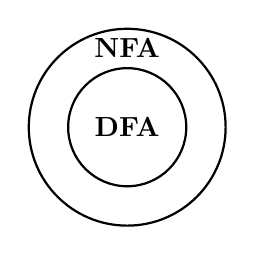
\begin{tikzpicture}
        % Cerchi per gli automi
        \draw[thick] (0, 0) circle (0.75cm) node[pos=0, yshift=0cm] {\textbf{DFA}};
        \draw[thick] (0, 0) circle (1.25cm) node[pos=0, yshift=1cm] {\textbf{NFA}};
    \end{tikzpicture} 
    \end{center}
    
}

Si vuole ora dimostrare che i \red{DFA sono tanto espressivi quanto gli NFA}, sebbene siano un loro sottoinsieme proprio

\mprop{}{
    Per ogni NFA, è prossibile costruire un DFA ad esso equivalente

}
\dimostrazione{
    Occorre seguire contemporaneamente tutti i possibili cammini alternativi dell'NFA di modo che gli stati del DFA che andranno a costruire sono costituiti sa insiemi di stati dell'NFA
}
Per dimostrare questa cosa occorre prima introdurre diversi concetti

\subsubsection{$\varepsilon$-closure}

\dfn{$\varepsilon$-closure}{
    L'\(\varepsilon\)-closure di uno stato \(q \in Q\), denotata come \(\varepsilon\text{-closure}(q)\), è definita come l'insieme degli stati \(q'\) tali che esiste un cammino da \(q\) a \(q'\) usando solo transizioni \(\varepsilon\), inclusivamente \(q\) stesso.

    In simboli:
    \[
        \varepsilon\text{-closure}(q) = \{ q' \in Q \mid q \xrightarrow{\varepsilon^*} q' \},
    \]

    In altre parole si puo defnire come il minimo insieme che rispetta le seguenti regole:
    \[
        \frac{}{\{q\}\subseteq \varepsilon\text{-closure}(q)}\quad\frac{p\in \varepsilon\text{-closure}(q)}{\delta(p,\varepsilon)\subseteq \varepsilon\text{-closure}(q)}    
    \]

}
nel caso abbiamo un insieme $P$ di nodi allarghiamo la definizione di $\varepsilon\text{-closure}$ a quella di:
\[
    \varepsilon\text{-closure}(P) = \bigcup_{p\in P}\varepsilon\text{-closure}(p)
\]

\esempio{
    Considera il seguente NFA:
    \begin{itemize}
        \item Stati: \(Q = \{q_0, q_1, q_2\}\)
        \item Transizioni:
        \begin{itemize}
            \item \(\delta(q_0, \varepsilon) = \{q_1\}\)
            \item \(\delta(q_1, \varepsilon) = \{q_2\}\)
            \item \(\delta(q_2, a) = \{q_2\}\)
        \end{itemize}
    \end{itemize}
    Il calcolo dell'\(\varepsilon\)-closure è presto fatto:
    \begin{itemize}
        \item \(\varepsilon\text{-closure}(q_0)\):
        \begin{itemize}
            \item Da \(q_0\), puoi raggiungere \(q_1\) attraverso una transizione \(\varepsilon\)
            \item Da \(q_1\), puoi raggiungere \(q_2\) attraverso un'altra \(\varepsilon\)
        \end{itemize}
        Quindi: \(\varepsilon\text{-closure}(q_0) = \{q_0, q_1, q_2\}\)
        \item  \(\varepsilon\text{-closure}(q_1)\):
        \begin{itemize}
            \item  Da \(q_1\), puoi raggiungere \(q_2\) attraverso una transizione \(\varepsilon\)
        \end{itemize}
        Quindi: \(\varepsilon\text{-closure}(q_1) = \{q_1, q_2\}\)
        \item \(\varepsilon\text{-closure}(q_2)\):
        \begin{itemize}
            \item \(q_2\) non ha transizioni \(\varepsilon\) in uscita
        \end{itemize}
        Quindi: \(\varepsilon\text{-closure}(q_2) = \{q_2\}\)
    \end{itemize}

}

Qui è presentato l'algoritmo per calcolare la $\varepsilon$-closure:
\begin{algorithm}
    \caption{$\varepsilon$-closure}
    \KwIn{Stato $p$}
    \KwOut{insieme di stati raggiungibili da $p$ con mosse $\varepsilon$}

    $T\gets P$\tcp*{inizalizzazione}
    $\varepsilon$-closure($p$) = P\tcp*{inizalizzazione}

    \While{$T\neq \varnothing$}{
        scegli un $r\in T$ e rimuovilo da $T$\;
        \ForEach{$s\in\delta(r,\varepsilon)$}{
            \If{$s\neq\varepsilon$-closure($p$)}{
                add $s$ to $\varepsilon$-closure($p$)\;
                add $s$ to T\;
            }
        }
    }
\end{algorithm} 
\clm{}{}{
    usando le $\varepsilon$-closure. si può definire il linguaggio riconosciuto da un NFA in modo elegante. 
    
    Definiamo la seguente funzione
    \[
        \hat{\delta}:Q\times \Sigma^* \mathcal{Q}(P)
    \]
    per in induzione
    \[
        \hat{\delta}(q,\varepsilon) = \epsilon\text{-closure}(q)
    \]
    \[
        \hat{\delta}(q,xa) = \varepsilon\text{-closure}(q) \text{ dove }P=\{p\in Q\mid \exists r\in \hat{\delta}(q,x)\land p\in (r,a)\}
    \]
    

    Pertanto si può dimostrare (dimostrazione difficile) che:
    \[
        w\in L[N] \iff \exists p \in F t.c. p\in \hat{\delta}(q_0,w)
    \]
}
\subsubsection{funzione mossa}
\dfn{
    funzione mossa
}{
    Si definisce la \textbf{funzione mossa} come estensione della funzione di transizione $\delta$ di un NFA come:
    \[
        \begin{array}{l}
            mossa:\mathcal{P}(Q)\times \Sigma\to \mathcal{P}(Q)\\
            mossa(P,a) = \bigcup_{p\in P}\delta (p,a)
        \end{array}
    \]
    Cioe l’insieme delle mosse $a$ da un insieme di nodi $P$ e l’unione di tutte le mosse $a$ di ogni nodo dell’insieme. `
}

\subsubsection{funzione transazione}
\dfn{funzione transizione}{
    Si definisce \textbf{transizione} e la si denota con $\Delta$ tale funzione:
    \[ 
        \Delta(A,b)=\varepsilon\text{-closure}(mossa(A,b)) 
    \]
    Con $A$ un insieme di stati e $b$ una transizione
}

\subsubsection{costruzione per sottoinsiemi del DFA}
Qua di seguito l’algoritmo per la costruzione di sottoinsiemi, che serve per passare da un NFA a un DFA equivalente

\begin{algorithm}
    \caption{costruzionePerSottoinsiemi()}
    \KwIn{NFA $N=(\Sigma, Q,\delta,q_0,F)$}
    \KwOut{DFA $M_N=(\Sigma,T,\Delta, \varepsilon\text{-closure}(q_0), \mathcal{F})$}
    $S\gets\varepsilon\text{-closure}(q_0)$\tcp*{stato iniziale del DFA}
    $T=\{S\}$\tcp*{$T$ è il l'insieme degli stati del DFA}
    \While{c'è un $P\in T$ non marcato}{
        marca $P$\;
        \ForEach{$a\in\Sigma$}{
            $R\gets \varepsilon\text{-closure}(mossa(P,a))$\;
            \If{$R\notin T$}{
                add $R$ to $T$\tcp*{$R$ non ha marca}
                definisci $\Delta(P,a) = R$\;
        }
    }
}
\end{algorithm}

Definiamo quindi il DFA equivalente:
\dfn{DFA quivalente}{
    Si definisce il DFA equivalente tale automa:
    \[
        M_n = (\Sigma, T,\Delta, \varepsilon\text{-closure}(q_0), \mathcal{F})    
    \]
    dove $R\in \mathcal{F}\iff \exists q\in R$ con $q\in F$
}

Si può notare come l'algoritmo che definisce la funzione di transizione (vista poch'anzi) rispetta le limitazioni dei DFA: non ci sono mosse epsilon e per ogni caraere dell’alfabeto esiste una ed
una sola mossa in qualunque stato
\esempio{
    Consideriamo l’NFA seguente (relativo all’espressione regolare $((a|b)^*ab)$:
    \begin{center}
        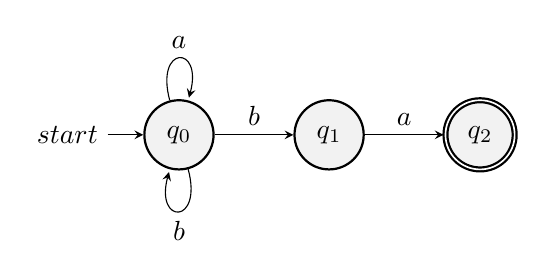
\begin{tikzpicture}[node distance=1cm]
        \node[state, initial] (q0) {$q_0$};
        \node[state] (q1) [right=of q0] {$q_1$};
        \node[state, accepting] (q2) [right=of q1] {$q_2$};

        % Transizioni
        \path[->]
        (q0) edge[loop above] node {$a$} ()
            edge[loop below] node {$b$} ()
            edge[above] node {$b$} (q1)
        (q1) edge node[above] {$a$} (q2);
    \end{tikzpicture}
    \end{center}
    

    Vogliamo ora trovare un DFA equivalente ad esso, applichiamo l’algoritmo di costruzioni per sottoinsiemi:
    \begin{itemize}
        \item calcoliamo lo stato iniziale $S=\varepsilon\text{-closure}(q_0)$, che è $S=q_0$. 
        \item Creiamo $T$ e gli inseriamo $S$ marcandolo
        \item Per ogni simbolo dobbiamo calcolare $\varepsilon\text{-closure}(mossa(P,a))$, ma visto che l'alfabeto è $\{a,b\}$ lo facciamo 2 volte:
        \begin{itemize}
            \item per il carattere $a$ calcoliamo con $P=S=\{q_0\}$:
              \[
                \begin{array}{l}
                    R = \varepsilon\text{-closure}(mossa(P,a)) = \epsilon\text{-closure}\left(\bigcup_{p\in\{q_0\}}\delta (p,a)\right)\\
                    =\varepsilon\text{-closure}(\delta(q_0,a)) =\epsilon\text{-closure}(\{q_0\}) =\{q_0\}
                \end{array}
              \]
                 
            Si definisca $\delta(S,a)=\{q_0\}$ e visto che $\{q_0\}\in T$ non lo andiamo a ri-aggiungere
            \item per il carattere $a$ calcoliamo con $P=S=\{q_0\}$:
              \[
                \begin{array}{l}
                    R = \varepsilon\text{-closure}(mossa(P,b)) = \epsilon\text{-closure}\left(\bigcup_{p\in\{q_0\}}\delta (p,b)\right) \\                
                    =\varepsilon\text{-closure}(\delta(q_0,b)) =\epsilon\text{-closure}(\{q_0, q_1\}) =\{q_0,q_1\}
                \end{array}
              \]
            visto che $\{q_0,q_1\}\notin T$ lo andiamo ad aggiungere
        \end{itemize}
        \item si calcoli ora con $P=\{q_0, q_1\}$ andando a calcolare la stessa cosa:
        \begin{itemize}
            \item per $a$ si ha:
              \[
                \begin{array}{l}
                    R=    \varepsilon\text{-closure} (mossa(P,a)) = \epsilon\text{-closure}\left(\bigcup_{p\in\{q_0, q_1\}}\delta(p,a)\right)\\                 
                    = \varepsilon\text{-closure} (\{q_0\}\cup\{ q_2\}) = \{q_0,q_2\}
                \end{array}
              \]
            quindi $\Delta(\{q_0,q_1\}, a)=\{q_0,q_2\}$. Visto $\{q_0,q_2\}\notin T$ lo aggiungiamo 
            \item  per $b$ si ha $R=\{q_0,q_1\}$. Quindi $\Delta(\{q_0, q_1\}, b) = \{q_0,q_1\}$ e non lo si raggiunge
        \end{itemize}
        \item ripetiamo per $P=\{q_0, q_2\}$ (salto i calcoli)
    \end{itemize}

    alla fine di sto ambaradam si ottiene $DFA \;N'=(\Sigma, \{\{q_0\},\{q_0,q_1\}, \{q_0,q_2\}\}, \Delta, \{q_0\}, \{q_0,q_2\})$ che in forma di diagramma di transizione e:
    \begin{center}
        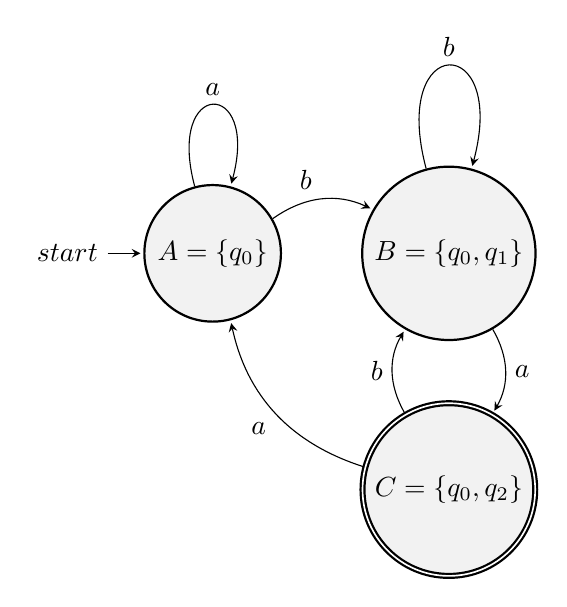
\begin{tikzpicture}[shorten >=1pt, node distance=3cm, on grid, auto]

            % Stati
            \node[state, initial] (q0) {$A=\{q_0\}$};
            \node[state] (q1) [right=of q0] {$B=\{q_0, q_1\}$};
            \node[state, accepting] (q2) [below=of q1] {$C=\{q_0, q_2\}$};
        
            % Transizioni
            \path[->]
                (q0) edge[loop above] node {$a$} () % loop su q0 con "a"
                     edge[bend left] node {$b$} (q1) % da q0 a q1 con "b"
                (q1) edge[loop above] node {$b$} () % loop su q1 con "b"
                     edge[bend left] node {$a$} (q2) % da q1 a q2 con "a"
                (q2) edge[bend left] node {$b$} (q1) % da q2 a q1 con "b"
                     edge[bend left] node {$a$} (q0); % da q2 a q0 con "a"
        
        \end{tikzpicture}
            \end{center}
}

esempio bello corposo:
\esempio{
    \begin{center}
        \begin{tikzpicture}[shorten >=1pt, node distance=2cm, on grid, auto]
            % Stati
            \node[state, initial] (q0) {$q_0$};
            \node[state] (q2) [right of=q0] {$q_2$};
            \node[state, accepting] (q4) [right of=q2] {$q_4$};
            \node[state] (q1) [above of=q1] {$q_1$};
            \node[state] (q3) [right of=q1] {$q_3$};
        
            % Transizioni
            \path[->]
                (q0) edge[bend left] node {$\varepsilon$} (q1)
                     edge node[below] {$b$} (q2)
                (q1) edge node {$a$} (q0)
                     edge node {$\varepsilon$} (q2)
                     edge node {$\varepsilon$} (q3)
                     edge node {$a$} (q4)
                (q2) edge node[below] {$b$} (q4)
                (q3) edge[bend left] node {$a$} (q4)
                (q4) edge[bend left] node {$\varepsilon$} (q3);
        \end{tikzpicture}
        \end{center}
        
        si noti i seguenti calcoli

        \vspace{0.5cm}
        \begin{math}
            A = \varepsilon\text{-closure}(q_0) = \{q_0, q_1, q_2, q_3\} \\
            \Delta(A, a) = \varepsilon\text{-closure}(\text{move}(A, a)) = \epsilon\text{-closure}(\{q_0, q_4\}) = \{q_0, q_1, q_2, q_3, q_4\} = B \\
            \Delta(A, b) = \varepsilon\text{-closure}(\text{move}(A, b)) = \epsilon\text{-closure}(\{q_2, q_3, q_4\}) = \{q_2, q_3, q_4\} = C \\
            \Delta(B, a) = \varepsilon\text{-closure}(\text{move}(B, a)) = \epsilon\text{-closure}(\{q_0, q_4\}) = B \\
            \Delta(B, b) = \varepsilon\text{-closure}(\text{move}(B, b)) = \epsilon\text{-closure}(\{q_2, q_4\}) = C \\
            \Delta(C, a) = \varepsilon\text{-closure}(\text{move}(C, a)) = \epsilon\text{-closure}(\{q_4\}) = \{q_3, q_4\} = D \\
            \Delta(C, b) = \varepsilon\text{-closure}(\text{move}(C, b)) = \epsilon\text{-closure}(\{q_4\}) = D \\
            \Delta(D, a) = \varepsilon\text{-closure}(\text{move}(D, a)) = \epsilon\text{-closure}(\{q_4\}) = \varnothing = D \\
            \Delta(D, b) = \varepsilon\text{-closure}(\text{move}(D, b)) = \epsilon\text{-closure}(\varnothing) = \varnothing = E \\
            \Delta(E, a) = \varepsilon\text{-closure}(\text{move}(E, a)) = \epsilon\text{-closure}(\varnothing) = \varnothing = E \\
            \Delta(E, b) = \varepsilon\text{-closure}(\text{move}(E, b)) = \epsilon\text{-closure}(\varnothing) = \varnothing = E
        \end{math}
        \vspace{0.5cm}

        il cui DFA $M_N$ è:
        
        \begin{center}
        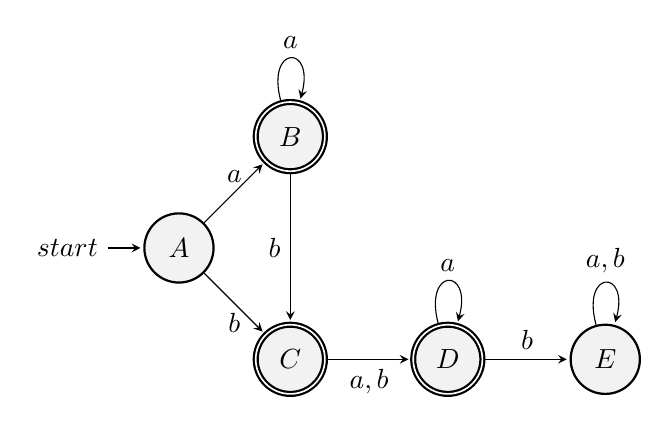
\begin{tikzpicture}[shorten >=1pt, node distance=2cm, on grid, auto]
            % Stati
            \node[state, initial] (A) {$A$};
            \node[state, accepting] (B) [above right=of A] {$B$};
            \node[state, accepting] (C) [below right=of A] {$C$};
            \node[state, accepting] (D) [right=of C] {$D$};
            \node[state] (E) [right=of D] {$E$};
        
            % Transizioni
            \path[->]
                (A) edge[above] node {$a$} (B)
                    edge[above] node[below] {$b$} (C)
                (B) edge[loop above] node {$a$} ()
                    edge node[left] {$b$} (C)
                (C) edge[below] node {$a,b$} (D)
                (D) edge[above] node {$b$} (E)
                    edge[loop above] node {$a$} ()
                (E) edge[loop above] node {$a, b$} ();
        \end{tikzpicture}
        \end{center}
}

\subsubsection{casi pessimi}

\clm{}{
    Vi sono tuttavia casi pessimi in cui il DFA equivalente è esponenzialmente più grande di del DFA, ovvero che se il NFA $N$ ha $n$ stati il suo $M_n$ può averne $2^n$
}

\esempio{
        Sia $N$ il seguente NFA con 2 stati:
        \begin{center}
            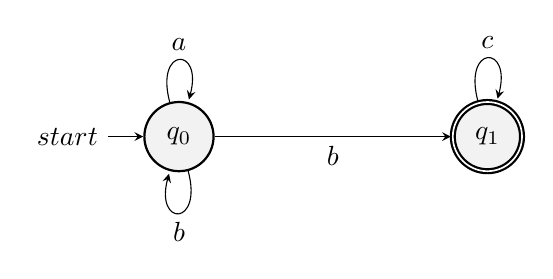
\begin{tikzpicture}
            \node[state, initial] (q0) {$q_0$};
            \node[state, accepting] (q1) [right=of q0] {$q_1$};

            \path[->]
                (q0) 
                    edge node[below] {$b$} (q1)
                    edge[loop below] node {$b$} ()
                    edge[loop above] node {$a$} ()
                (q1) 
                    edge[loop above] node {$c$} (); 
        \end{tikzpicture}
        \end{center}
        

        per costruire il suo $M_N$ si hanno i seguenti nodi
        \begin{itemize}
            \item $A=\{q_0\}$
            \item $B=\{q_0, q_1\}$
            \item $A=\{q_1\}$
            \item $D=\varnothing$
        \end{itemize} 

        in diagramma di transazione diventa:
        \begin{center}
            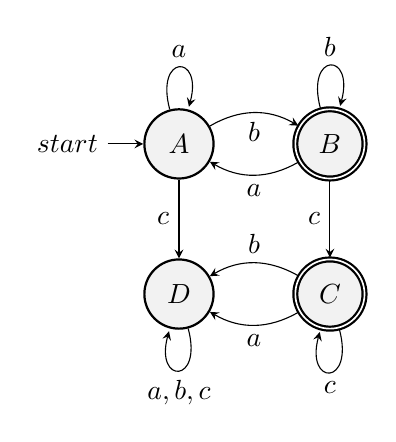
\begin{tikzpicture}[node distance=1cm]
            \node[state, initial] (a) {$A$};
            \node[state, accepting] (b) [right=of a] {$B$};
            \node[state] (d) [below=of a] {$D$};
            \node[state, accepting] (c) [right=of d] {$C$};

            \path[->]
                (a) 
                    edge[bend left] node[below] {$b$} (b)
                    edge[loop above] node {$a$} ()
                    edge[above] node[left] {$c$} (d)
                (b) 
                    edge[loop above] node {$b$} ()
                    edge[above] node[left] {$c$} (c)
                    edge[bend left] node[below] {$a$} (a)
                (d) 
                    edge[loop below] node {$a,b,c$} ()
                (c) 
                    edge[loop below] node {$c$} ()
                    edge[bend right] node[above] {$b$} (d)
                    edge[bend left] node[below] {$a$} (d);
        \end{tikzpicture}
        \end{center}
        

}



Adesso si può dimostrare il teorema dell'equivalenza
\subsubsection{teorema d'equivalenza tra NFA e DFA}

\thm{
    Bonzo-GioLaPalma
}{
    Sia $N=(\Sigma, Q,\delta,q_0, F)$ un NFA  e sia $M_n$ l'automa ottenuto con la costruzione per sottoinsiemi. allora $M_n$ è un DFA e si ha che 
    \[
        L[N]=L[M_n]    
    \]
    In altre parole, $ N $ e $ M_n $ sono equivalenti.
}
\dimostrazione{
    Sia \( N = (Z, \Sigma, \delta, q_0, F) \) un NFA e sia \( M_N = (\Gamma, \Sigma, \Delta, A, F') \) l'automa ottenuto con l'algoritmo.

\begin{itemize}
    \item \( M_N \) è \textbf{deterministico}: Infatti $\Delta(A, a)$ con $A\in T\land a\in \Sigma$ è definita in modo univoco 
        

    \item  Quindi mi riduco a dimostrare che $L[N]=L[M_n]$
    \begin{itemize}
        \item si osservi che per un DFA, $\varepsilon$-closure$(R)=R$
        \item chiamiamo $i_m=\varepsilon$-closure$(q_0)$ lo stato iniziale di $M_n$
    \end{itemize}
\end{itemize}



Vogliamo dimostrare che $\forall w\in \Sigma^*$

\[
\delta(q_0, w) = \Delta(A, w) 
\]
per induzione sulla lunghezza di $w$
\begin{itemize}
    \item \textbf{Caso base}: \( |w| = 0 \text{ cioè } w=\varepsilon \):
    \[
        \hat{\delta}(A, \varepsilon) = \epsilon\text{-closure}(q_0)
    \]
    \[
        \hat{\Delta} (i_m,\varepsilon) =     \epsilon\text{-closure}(i_m)= i_M=<\epsilon\text{-closure}(q_0)
    \]
    \item \textbf{Caso induttivo}:\( w = xa \) con \( x \in \Sigma^*, a \in \Sigma \)
    Per ipotesi induttiva, sappiamo che:
    \[
        \hat{\delta}(q_0, x) = \Delta(\{q_0\}, x) = \{p_1, \dots, p_k\}
    \]
    
    Per definizione di \(\hat{\delta}\):
    \[
        \hat{\delta}(q_0, xa) = \Delta\big(\varepsilon\text{-closure}\big(\bigcup_{i=1}^{k} \delta(p_i, a)\big)\big)
    \]
    
    Similmente:
    \[
        \Delta(\{q_0\}, xa) = \Delta(\{p_1, \dots, p_k\}, a)
    \]
    
    In base all'algoritmo, la definizione di \(\Delta\) ci dice che:
    \[
        \Delta(\{p_1, \dots, p_k\}, a) = \varepsilon\text{-closure}\big(\text{mossa}(\{p_1, \dots, p_k\}, a)\big)= \varepsilon\text{-closure}\big(\bigcup_{i=1}^{k} \delta(p_i, a)\big)= \hat{\delta}(q_0, xa)
    \]
    OK.
    
    ---
    
    Infine, abbiamo che:
    \[
        w \in L[N] \iff \exists p \in \hat{\delta}(q_0, w) \text{ con } p \in F
    \]
    
    \[
        \iff \exists p \in \Delta(i_H, w) \text{ con } p \in F
    \]
    
    \[
        \iff w \in L[M_N] \quad \forall w \in \Sigma^*
    \]
    
    Quindi:
    \[
        L[N] = L[M_N] \quad \text{c.v.d.}
    \]
    
\end{itemize}

}

\subsection{Da espressioni regolarei a NFA equivalenti}

\thm{Basta - Dario è sVenuto}{
    Data un'espressione regolare $S$, possiamo costruire un NFA $N[s]$ tale che:
    \[
        \mathcal{L}[s] = L[N[s]]
    \]

    ovvero un linguaggio individuato da un linguaggio regolare è equivalente ad un linguaggio riconosciuto da un automa non deterministico a stati finiti costruito a partire da $S$, questo significa che \red{gli NFA riconoscono TUTTI i linguaggi regolari}, vedremo poi che riconoscono solo i linguaggi regolari
}
\dimostrazione{
    Dimostreremo il teorema per induzione sulla sintassi astratta della espressione regolare $S$.

    Si costruisca un possibile NFA associato all'espressione regolare $S$, in modo da mantenere i seguente due invarianti:
    \begin{itemize}
        \item lo stato iniziale non ha archi entranti
        \item $N[s]$ ha un solo stato finale senza archi uscenti
    \end{itemize}

    Procedo ad esaminare i vari casi 
    \begin{itemize}
        \item Sia $s=\varnothing$
        
        In questo caso sarà possibile costruire un NFA con due stati (iniziale e finale) non connessi, quindi $N[s]$:
        \begin{center}
            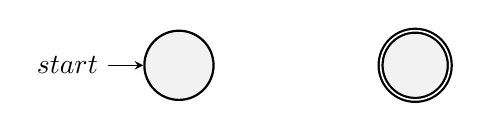
\begin{tikzpicture}
                \node[state, initial] (A) {};
                \node[state, accepting] (B) [right of=A] {};
            \end{tikzpicture}
        \end{center}
        Si osservi che $\mathcal{L}[\varnothing]=\varnothing=L[N[s]]$
        \item Sia $s=\varepsilon$
        
        In questo caso sarà possibile costruire un NFA con due stati (iniziale e finale) connessi da un $\varepsilon$, quindi $N[s]$:

        \begin{center}
            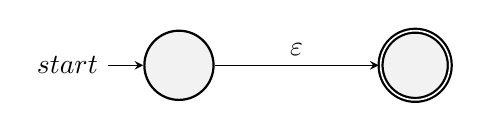
\begin{tikzpicture}
                \node[state, initial] (A) {};
                \node[state, accepting] (B) [right of=A] {};

                \path[->]
                    (A) edge[above] node{$\varepsilon$} (B);
            \end{tikzpicture}


        \end{center}
        Si osservi che, in questo caso, $\mathcal{L}[\varepsilon] = \{\epsilon\}=L[N[s]]$
        \item Sia $S = a$
        
        In questo caso sarà possibile costruire un NFA con due stati (iniziale e finale) connessi da una transizione $a$, quindi $N[s]$:

        \begin{center}
            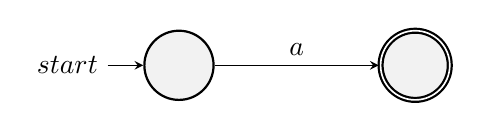
\begin{tikzpicture}
                \node[state, initial] (A) {};
                \node[state, accepting] (B) [right of=A] {};

                \path[->]
                    (A) edge[above] node{$a$} (B);
            \end{tikzpicture}
        \end{center}

        Si osservi che, in questo caso, $\mathcal{L}[a] = \{a\}=L[N[s]]$
        \item caso $s= r|t$
        
        Ipotizziamo di avere già costruito gli automi $N[t]$ ed $N[r]$, per costruire "l'or" è possibile partire da uno stato iniziale $i$ e collegarlo con transizioni $\varepsilon$ ai due automi, da entrambi si confluisce in uno stato finale $f$ con transazioni $\epsilon$
        
        \begin{center}
            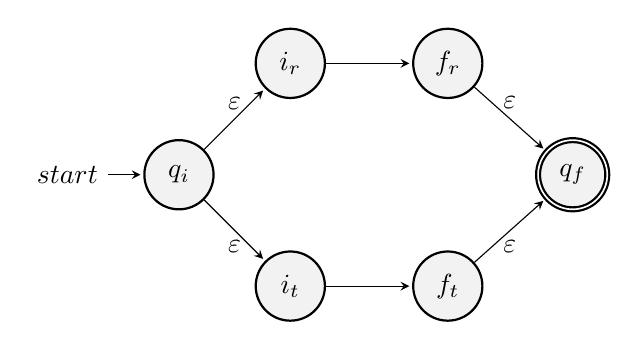
\begin{tikzpicture}[shorten >=1pt, node distance=2cm, on grid, auto]
                % Stati
                \node[state, initial] (qi) {$q_i$};
                \node[state] (ir) [above right=of qi] {$i_r$};
                \node[state] (fr) [right=of ir] {$f_r$};
                \node[state] (it) [below right=of qi] {$i_t$};
                \node[state] (ft) [right=of it] {$f_t$};
                \node[state, accepting] (qf) [right=5cm of qi] {$q_f$};
            
                % Transizioni
                \path[->]
                (qi) edge[above] node {$\varepsilon$} (ir)
                     edge[below] node {$\varepsilon$} (it)
                (ir) edge[above] (fr)
                (fr) edge[above] node {$\varepsilon$} (qf)
                (it) edge[above] (ft)
                (ft) edge[below] node {$\varepsilon$} (qf);

                %TODO inserire cerchi per contenere gli automi
                
            \end{tikzpicture}
            
        \end{center}

        Algebricamente si può dimostrare che $\mathcal{L}[r|t]=\mathcal{L}[t]\cup \mathcal{L}[r]$

        e per ipotesi induttiva si ha:
        \[
            \mathcal{L}[t]\cup \mathcal{L}[r] =L[N[r]]\cup L[N[t]] =L[N[r|t]]
        \]
        \item Sia $s=r\cdot t$
        
        Ipotizziamo di avere già costruito gli automi $N[t]$ ed $N[r]$, per costruire la concatenazione è possibile fondere lo stato finale del primo automa con quello del secondo automa, si ha, quindi, che $N[s]$:

        \begin{center}
            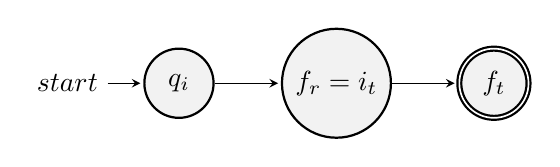
\begin{tikzpicture}
                [shorten >=1pt, node distance=2cm, on grid, auto]
                % Stati
                \node[state, initial] (ir) {$q_i$};
                \node[state] (frit) [right=of ir] {$f_r = i_t$};
                \node[state, accepting] (ft) [right=of frit] {$f_t$};
                
                % Transizioni
                \path[->]
                    (ir) edge (frit)
                    (frit) edge (ft);
            \end{tikzpicture}            
        \end{center}

        %TODO inserire cerchi per gli automi probabile libreria FIT

        \item Sia $s=r^*$
        
        Ipotizzando di aver già costruito $N[r]$ è possibile costruire l'automa creando un ciclo $\varepsilon$ dalla fine di $N[r]$ al suo inizio

        \begin{center}
            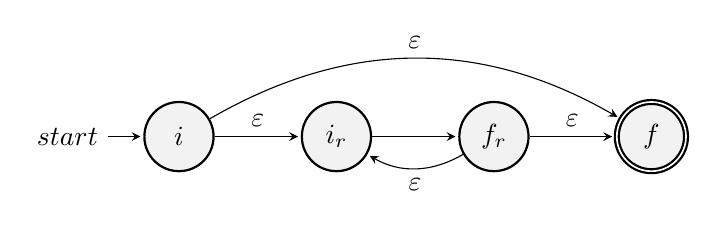
\begin{tikzpicture}
                [shorten >=1pt, node distance=2cm, on grid, auto]
                % Stati
                \node[state, initial] (i) {$i$};
                \node[state] (it) [right=of i] {$i_r$};
                \node[state] (ft) [right=of it] {$f_r$};
                \node[state, accepting] (f) [right=of ft] {$f$};

                
                % Transizioni
                \path[->]
                    (i) edge node {$\varepsilon$} (it)
                        edge[bend left] node {$\varepsilon$} (f)
                    (it) edge (ft)
                    (ft) 
                        edge node {$\varepsilon$} (f)
                        edge[bend left] node {$\varepsilon$} (it);
                    
            \end{tikzpicture}            
        \end{center}

        Si osservi che:

        \[
            \mathcal{L}[r^*] = (\mathcal{L}[r])^* 
        \]
        per ipotesi induttiva

        \[
            (\mathcal{L}[r])^* = (L[N[r]])^* = L[N[r^*]]
        \]
    \end{itemize}
}
\esempio{
    Sia $S= (a|b^*)ba$ un'espressione regoalre e costruiamnone l'albero sintattico

    \begin{center}
       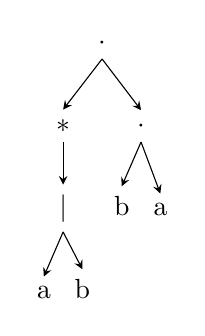
\begin{tikzpicture}
        \Tree[
                .$\cdot$
                [
                    .$*$
                    [
                        .$|$
                        a
                        b
                    ]
                ]
                [
                    .$\cdot$
                    b
                    a
                ]
        ]
    \end{tikzpicture} 
    \end{center}

    Partiamo dalle foglie e risaliamo alla radice (bottom-up)
    Si ha:

    \begin{itemize}
        \item $N[a]$:
        \begin{center}
            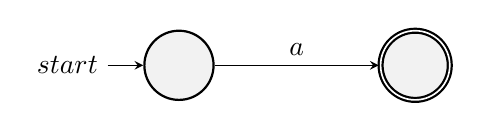
\begin{tikzpicture}
                \node[state, initial] (A) {};
                \node[state, accepting] (B) [right of=A] {};

                \path[->]
                    (A) edge[above] node{$a$} (B);
            \end{tikzpicture}
        \end{center}

        \item $N[b]$:
        \begin{center}
            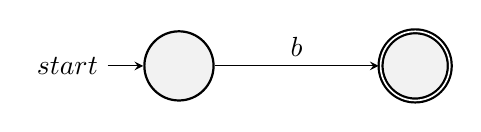
\begin{tikzpicture}
                \node[state, initial] (A) {};
                \node[state, accepting] (B) [right of=A] {};

                \path[->]
                    (A) edge[above] node{$b$} (B);
            \end{tikzpicture}
        \end{center}

        \item  $N[a|b]$:
        
        \begin{center}
            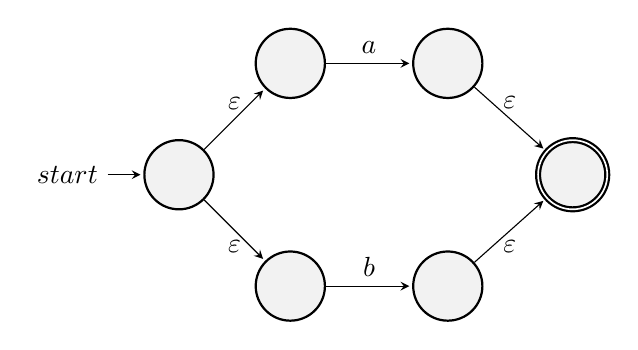
\begin{tikzpicture}[shorten >=1pt, node distance=2cm, on grid, auto]
                % Stati
                \node[state, initial] (qi) {};
                \node[state] (ir) [above right=of qi] {};
                \node[state] (fr) [right=of ir] {};
                \node[state] (it) [below right=of qi] {};
                \node[state] (ft) [right=of it] {};
                \node[state, accepting] (qf) [right=5cm of qi] {};
            
                % Transizioni
                \path[->]
                (qi) edge[above] node {$\varepsilon$} (ir)
                     edge[below] node {$\varepsilon$} (it)
                (ir) edge[above] node {$a$} (fr)
                (fr) edge[above] node {$\varepsilon$} (qf)
                (it) edge[above] node {$b$} (ft)
                (ft) edge[below] node {$\varepsilon$} (qf);

                %TODO inserire cerchi per contenere gli automi
                
            \end{tikzpicture}
            
        \end{center}

        \item  $N[(a|b)^*]$:
        
        \begin{center}
            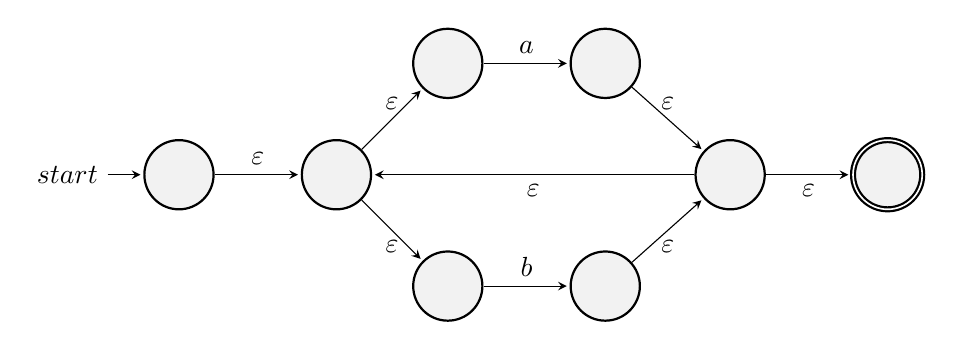
\begin{tikzpicture}[shorten >=1pt, node distance=2cm, on grid, auto]
                % Stati
                \node[state, initial] (i) {};
                \node[state] (qi) [right=of i] {};
                \node[state] (ir) [above right=of qi] {};
                \node[state] (fr) [right=of ir] {};
                \node[state] (it) [below right=of qi] {};
                \node[state] (ft) [right=of it] {};
                \node[state] (qf) [right=5cm of qi] {};
                \node[state, accepting] (f) [right=of qf] {};
            
                % Transizioni
                \path[->]
                (i) edge[above] node {$\varepsilon$} (qi)
                (qi) edge[above] node {$\varepsilon$} (ir)
                     edge[below] node {$\varepsilon$} (it)
                (ir) edge[above] node {$a$} (fr)
                (fr) edge[above] node {$\varepsilon$} (qf)
                (it) edge[above] node {$b$} (ft)
                (ft) 
                    edge[below] node {$\varepsilon$} (qf)
                    
                (qf) edge[below] node {$\varepsilon$} (f)
                    edge[below] node {$\varepsilon$} (qi);

            \end{tikzpicture}
            
        \end{center}
        \item $N[ba]$:
        \begin{center}
            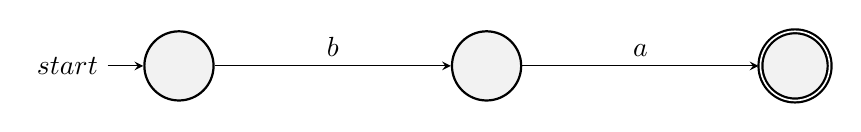
\begin{tikzpicture}
                \node[state, initial] (A) {};
                \node[state] (B) [right=of A] {};
                \node[state, accepting] (C) [right=of B] {};

                \path[->]
                    (A) edge[above] node{$b$} (B)
                    (B) edge[above] node{$a$} (C);
            \end{tikzpicture}
        \end{center}

        \item $N[s]$:
        \begin{center}
            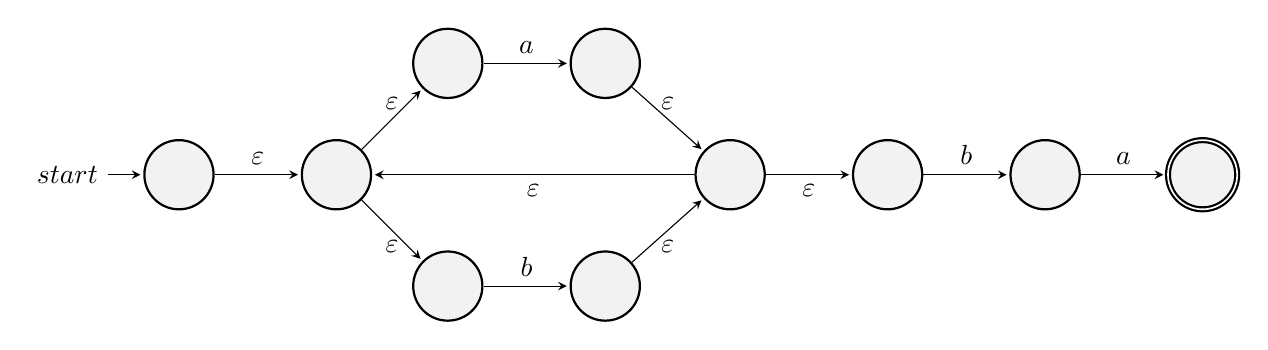
\begin{tikzpicture}[shorten >=1pt, node distance=2cm, on grid, auto]
                % Stati
                \node[state, initial] (i) {};
                \node[state] (qi) [right=of i] {};
                \node[state] (ir) [above right=of qi] {};
                \node[state] (fr) [right=of ir] {};
                \node[state] (it) [below right=of qi] {};
                \node[state] (ft) [right=of it] {};
                \node[state] (qf) [right=5cm of qi] {};
                \node[state] (f) [right=of qf] {};
                \node[state] (B) [right=of f] {};
                \node[state, accepting] (C) [right=of B] {};
            
                % Transizioni
                \path[->]
                (i) edge[above] node {$\varepsilon$} (qi)
                (qi) edge[above] node {$\varepsilon$} (ir)
                     edge[below] node {$\varepsilon$} (it)
                (ir) edge[above] node {$a$} (fr)
                (fr) edge[above] node {$\varepsilon$} (qf)
                (it) edge[above] node {$b$} (ft)
                (ft) 
                    edge[below] node {$\varepsilon$} (qf)
                    
                (qf) 
                    edge[below] node {$\varepsilon$} (f)
                    edge[below] node {$\varepsilon$} (qi)
                (f) edge[above] node{$b$} (B)
                (B) edge[above] node{$a$} (C);

            \end{tikzpicture}
            
        \end{center}


        
    \end{itemize}

    


}

Altro esempietto:
\esempio{
        TODO da fare l'automa diretto qui

\[
\begin{aligned}
    &\text{Costruiamo il DFA associato a } N[s]: \\
    &A = \varepsilon\text{-closure}(0) = \{0\} \\
    &\Delta(A, a) = \varepsilon\text{-closure}(\{1\}) = \{1, 2, 3\} = B \\
    &\Delta(A, b) = \varepsilon\text{-closure}(\varnothing) = \varnothing = C \\
    &\Delta(B, a) = \varepsilon\text{-closure}(\{5\}) = \{5\} = D \\
    &\Delta(B, b) = \varepsilon\text{-closure}(\{3\}) = \{3, 4, 2\} = E \\
    &\Delta(D, a) = \varnothing = C, \quad \Delta(D, b) = \varnothing = C \\
    &\Delta(E, a) = \varepsilon\text{-closure}(\{5\}) = D, \quad \Delta(E, b) = \varepsilon\text{-closure}(\{3\}) = E \\
    &\Delta(C, a) = \varnothing = C, \quad \Delta(C, b) = \varnothing = C
\end{aligned}
\]

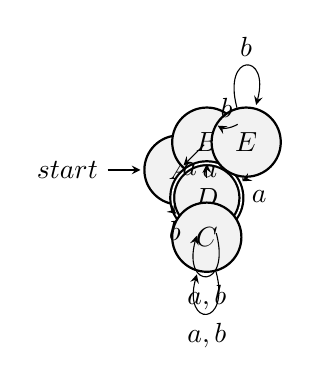
\begin{tikzpicture}[shorten >=1pt, node distance=0.5cm, on grid, auto]
    % Stati
    \node[state, initial] (A) {$A$};
    \node[state] (B) [above right=of A] {$B$};
    \node[state, accepting] (D) [below right=of A] {$D$};
    \node[state] (C) [below of=D] {$C$};
    \node[state] (E) [right=of B] {$E$};

    % Transizioni
    \path[->]
        (A) edge node {$a$} (B)
            edge[bend right] node[below] {$b$} (C)
        (B) edge node {$a$} (D)
            edge[bend left] node[above] {$b$} (E)
        (D) edge[loop below] node {$a,b$} (D)
        (C) edge[loop below] node {$a,b$} (C)
        (E) edge[loop above] node {$b$} (E)
            edge[bend left] node {$a$} (D);
\end{tikzpicture}

\[
\text{DFA associato a } N[a \; b^* \; a]
\]

}

\subsection{Da NFA a espressione regolare}
Aggiungo una dimostrazione presa dal libro di Michael Sipser, "Introduction to the Theory of Computation", che descrive come creare un'espressione regolare partendo direttamente da un NFA. Nella sezione successiva introdurremo le grammatiche regolari con le quali e' possibile dimostrare lo stesso teorema, quindi questa parte non e' necessaria ma solo un'idea interessante e piu' diretta.

Come anticipato precedentemente, e' possibile anche dimostrare la direzione inversa del teorema, ovvero che dato un NFA che riconosce un linguaggio $ L[N] $, e' sempre possibile generare un'espressione regolare che riconosca lo stesso linguaggio. Quindi vale il teorema generale:
\thm{Teoremone Piccolomini}{
  Un linguaggio e regolare sse esiste un automa a stati finiti che lo riconosce.
}
Sopra abbiamo gia dimostrato che preso un linguaggio regolare (ovvero descritto da un'espressione regolare) possiamo sempre costruire un NFA equivalente. Ci tocca dimostrare la direzione inversa, ovvero che preso un qualsiasi NFA, il linguaggio che riconosce e' regolare e quindi esiste un'espressione regolare che lo descrive.

Dato che abbiamo dimostrato col teorema Bonzo-GiolaPalma che un NFA e' sempre convertibile a un DFA, possiamo partire proprio da un DFA e definire un procedimento per ottenere un'espressione regolare equivalente. Dividiamo in due parti questo processo: prima convertiamo il DFA in un GNFA (General Nondeterministic Finite Automata), che ora defineremo, poi convertiamo il GNFA in un'ER.

\subsubsection{Automi finiti nondeterministici generali}
I GNFA sono praticamente dei NFA con funzione di transizione che funziona utilizzando le ER. Possono leggere blocchi alla volta dall'input, non solo caratteri, e se tale blocco soddisfa l' ER di una transizione che parte dallo stato corrente, allora si puo' seguire l'arco e cambiare stato. Ovviamente e' fortemente nondeterministico e possono esserci molti modi per elaborare la stessa sequenza di caratteri. 

\begin{center}
  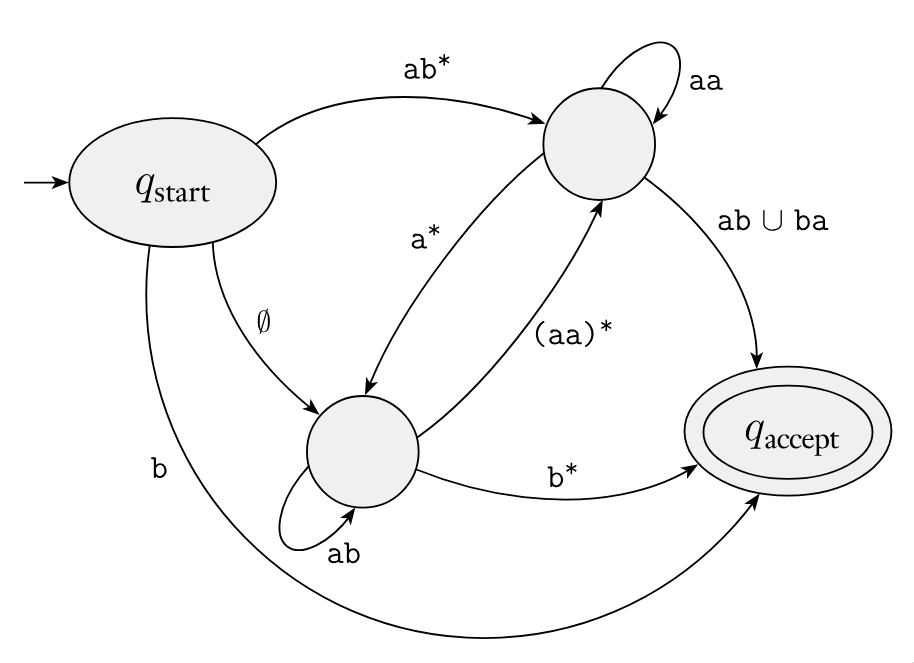
\includegraphics[scale=0.3]{img/2024-12-16-18-28-52.png}
\end{center}
Formalmente:
\dfn{GNFA}{
  Un \textbf{automa finito nondeterministico generale} e' una quintupla $ (Q, \Sigma, \delta, q_{\text{start}}, q_{\text{accept}}) $ tale che:
  \begin{itemize}
    \item $ Q $ e' un insieme finito di stati
    \item $ \Sigma $ e' l'alfabeto dell'input
    \item $ \delta: (Q - q_{\text{accept}}) \times (Q - q_{\text{start}}) \to \mathcal{R}_\Sigma $ e' la funzione di transizione
  \end{itemize}
  
  Dove $ \mathcal{R}_\Sigma $ e' l'insieme di tutte le ER sull'alfabeto $ \Sigma $.
}
 
Un GNFA riconosce una stringa $ w \in \Sigma^* $ se esitono una suddivisione $ w = w_1w_2...w_k $ con $ w_i \in \Sigma^* $ e una serie di stati $ q_0,q_1,...,q_k $ tali che:
\begin{enumerate}
  \item $ q_0 = q_{\text{start}} $
  \item $ q_k = q_{\text{accept}} $
  \item $ \forall i > 0. w_i \in \mathcal[R_i] $, dove $ R_i = \delta(q_{i-1}, q_i) $
\end{enumerate}


Per i fini della dimostrazione, ci interessiamo solo di GNFA specifici che rispettano le seguenti condizioni:
\begin{itemize}
  \item Lo stato iniziale ha archi che vanno verso tutti gli altri stati, ma nessuno entrante.
  \item Lo stato finale e' unico e ha archi entranti da tutti gli altri stati, ma nessuno uscente. Inoltre e' distinto dallo stato iniziale.
  \item Senza contare lo stato iniziale e lo stato finale, gli stati hanno archi che vanno verso tutti gli altri stati e anche verso loro stessi.
\end{itemize}

\subsubsection{Da DFA a GNFA}
Convertire un DFA in un GNFA in forma speciale e' semplice: basta aggiungere uno stato iniziale con arco $ \varepsilon $ verso lo stato iniziale vecchio, aggiungere uno stato finale con archi $ \epsilon $ entranti da tutti i vecchi stati finali e se ce piu' di un arco nella stessa direzione fra due nodi, fonderli insieme creando un unico arco la cui ER corrispondente e' l'unione delle ER dei vecchi archi. Infine, se mancano degli archi, aggiungere transizioni segnati dall'ER $ \emptyset $, che non puo' essere mai usata. 

\subsubsection{Da GNFA a ER}
Per ottenere l'ER a partire dal GNFA, l'idea principale e' la seguente:\\
Diciamo che il GNFA ha $ k $ stati. Sappiamo che $ k \geq 2 $ perche ci devono essere uno stato finale e uno iniziale distinti. Se riusciamo a rimuovere uno stato alla volta, che non sia finale o iniziale, mantenendo il nuovo GNFA appena ottenuto equivalente a quello prima, arriviamo ad un punto dove $ k=2 $ e l'automa e' costituito semplicemente da un arco che applica l'ER che ci porta dallo stato iniziale direttamente a quello finale, e che descrive quindi il linguaggio riconosciuto dal DFA iniziale.

Dobbiamo fare in modo che quando uno stato $ q_{\text{rip}} $ viene rimosso, le ER sugli archi vengano modificate in modo da simulare tutti i percorsi che sono stati rimossi. Quindi le nuove ER devono considerare sia le stringhe che portano direttamente dallo stato $ q_i $ allo stato $ q_j $, che le stringhe che portavano da $ q_i $ a $ q_j $ passando da $ q_{\text{rip}} $.

\begin{center}
  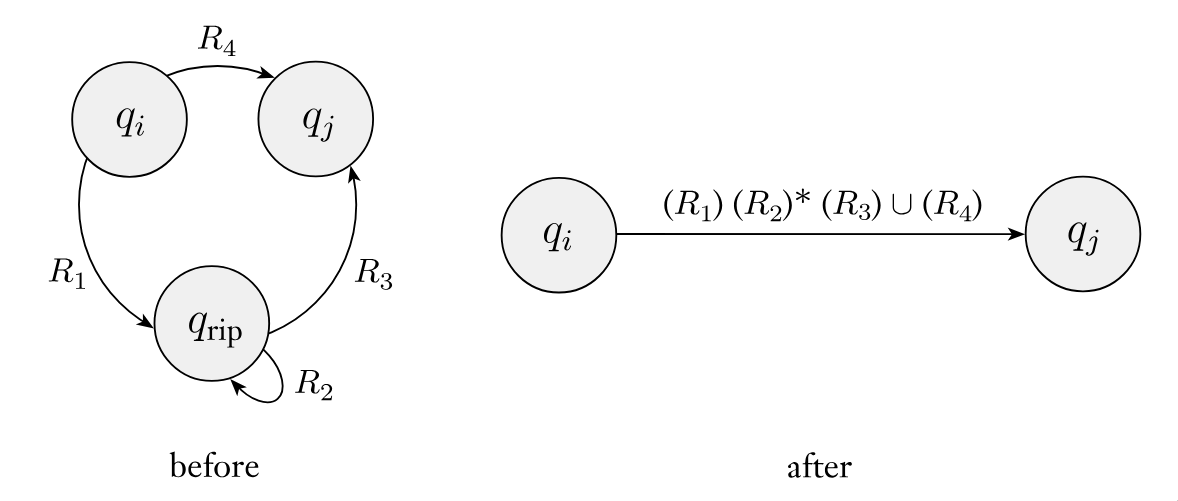
\includegraphics[scale=0.3]{img/2024-12-16-18-31-08.png}
\end{center}

Quindi, se nel vecchio GNFA:
\begin{enumerate}
  \item $ q_i $ va da $ q_{\text{rip}} $ per l'ER $ R_1 $
  \item $ q_{\text{rip}} $ va a se stesso per $ R_2 $
  \item $ q_{\text{rip}} $ va a $ q_j $ per $ R_3 $
  \item $ q_i $ va a $ q_j $ per $ R_4 $
\end{enumerate}
allora nel nuovo GNFA dobbiamo etichettare l'arco da $ q_i $ a $ q_j $ con l'ER:
\[
  (R_1)(R_2)^*(R_3)\cup (R_4)
\]
Ad ogni iterazione applichiamo questa trasformazione per ogni arco fra una coppia $ q_i q_j $ (anche quando $ i = j $). Formalizziamo tutto cio' (zio perone):
\pf{Dimostrazione formale}{
  Sia $ M $ il DFA equivalente all'NFA del teorema. Usando la procedura descritta sopra trasformiamo $ M $ in un GNFA $ G $. Usiamo la procedura ricorsiva CONVERT($ G $) per ottenere l'ER equivalente:
  \begin{enumerate}
    \item Sia $ k $ il numero di stati di $ G $
    \item Se $ k = 2 $, ritorna l'espressione regolare associata ai due nodi
    \item Se $ k > 2 $, seleziona uno stato $ q_{\text{rip}} \in Q $ che sia diverso dallo stato iniziale e finale e sia $ G' = (Q', \Sigma, \delta', q_{\text{start}}, q_{\text{accept}}) $ tale che:
      \begin{itemize}
        \item $ Q' = Q \setminus \{q_{\text{rip}}\} $
        \item $ \forall q_i \in Q' \setminus \{q_{\text{start}}\}, \forall q_j \in Q' \setminus \{q_{\text{accept}}\}: $
          \[
            \delta'(q_i, q_j) = (R_1)(R_2)^*(R_3)\cup(R_4)
          \]
          con $ R_1 = \delta(q_i, q_{\text{rip}}), R_2 = \delta(q_{\text{rip}}, q_{\text{rip}}), R_3 = \delta(q_{\text{rip}}, q_j), R_4 = \delta(q_i, q_j) $
      \end{itemize}
  \end{enumerate}

  Ora dimostriamo che CONVERT($ G $) ritorni il valore corretto. 

  Dimostriamo per induzione su $ k $, il numero di stati del GNFA $ G $:
  \begin{itemize}
    \item \textbf{Caso base:}

      Se $ k = 2 $, per la definizione di GNFA specifico abbiamo uno stato iniziale e un arco che lo collega allo stato finale. L'ER dell'arco descrive tutte le stringhe che portano $ G $ allo stato finale, quindi e' equivalente a $ G $.
    \item \textbf{Caso induttivo su $ k $:}

      Assumiamo che CONVERT($ G' $) equivale a $ G' $, dove $ G' $ e' il caso con $ k-1 $ stati. Dimostriamo che $ G' $ e $ G $ sono equivalenti. Prendiamo una parola $ w \in \Sigma^* $ accettata da $ G $. Quindi siano
      \[
      q_{\text{start}}, q_1, q_2, q_3, ..., q_{\text{accept}}
      \]
      la sequenza di stati di $ G $ di un percorso che accetta $ w $. Se $ q_{\text{rip}} $ (lo stato rimosso da $ G $ per creare $ G' $) non appartiene a questa sequenza, allora chiaramente $ w $ e' riconosciuto anche da $ G' $. Questo e' perche' i nuovi archi fra tutti gli stati mantengono l'ER originale tramite un'unione. Altrimenti, se $ q_{\text{rip}} $ fa parte del percorso, basta rimuovere tutte le evenienze dalla sequenza per trovare un percorso per cui $ G' $ accetta $ w $. Questo e' perche' nella definizione di CONVERT, facciamo in modo che le nuove ER fra due nodi considerino descrivino anche tutte le stringhe che portavano fra i due stati passando da $ q_{\text{rip}} $. 

      Al contrario, se $ G' $ riconosce $ w $, ad ogni arco e' associata un'ER che riconosce stringhe che in $ G $ fanno passare da $ q_i $ a $ q_i $ sia direttamente che tramite $ q_{\text{rip}} $. Quindi ovviamente anche $ G $ riconosce $ w $. Avendo dimostrato che $ G $ e $ G' $ sono equivalenti, possiamo usare l'ipotesi induttiva per dire che CONVERT($ G $) equivale a $ G $.
  \end{itemize}
}


\subsection{Chiusura dei linguaggi regolari rispetto alle operazioni regolari}
Per aiutarci ad architettare automi finiti o per distinguere linguaggi regolari da altri tipi di linguaggi che vedremo piu' avanti, puo' tornare utile sapere se sono chiusi rispetto alle operazioni regolari (concatenazione, unione, stella di Kleene). Generalmente, diciamo che un'insieme di oggetti e' chiusa rispetto a un'operazione se applicando quest'ultima a qualunque elemento dell'insieme, il risultato appartiene sempre allo stesso insieme. Quindi se consideriamo come macro-insieme l'insieme di tutti i linguaggi regolari e dimostriamo la chiusura rispetto a una certa operazione, allora siamo sicuri che il risultato di questa operazione applicata a linguaggi regolari sara' sempre un linguaggio regolare. Partiamo con l'operazione di unione:
\thm{Chiusura di linguaggi regolari rispetto all'unione}{
  La classe dei linguaggi regolari e' chiusa sotto l'unione.

  In altre parole, se $ A_1 $ e $ A_2 $ sono linguaggi regolari, lo e' anche $ A_1 \cup A_2 $.
}
Dato che abbiamo gia' dimostrato l'equivalenza fra DFA e NFA, possiamo usare il nondeterminismo per dimostrare il teorema sopra (e' possibile anche usare solo DFA, ma e' piu' lunga). L'idea della dimostrazione e' quella di creare due NFA, $ N_1, N_2 $ che riconoscono rispettivamente i linguaggi $ A_1, A_2 $, e poi di unirli per creare un nuovo NFA $ N $ che riconosca $ A_1 \cup A_2 $. Quindi, $ N $ deve riconoscere sia le stringhe di $ A_1 $ che di $ A_2 $. Creando un nuovo stato iniziale e collegandolo ai due stati iniziali di $ N_1 $ e $ N_2 $ con mosse $ \varepsilon $, quindi usando il nondeterminismo per accettare sia i casi in cui l'input appartiene ad $ A_1 $, sia quando appartiene ad $ A_2 $. 

\begin{center}
  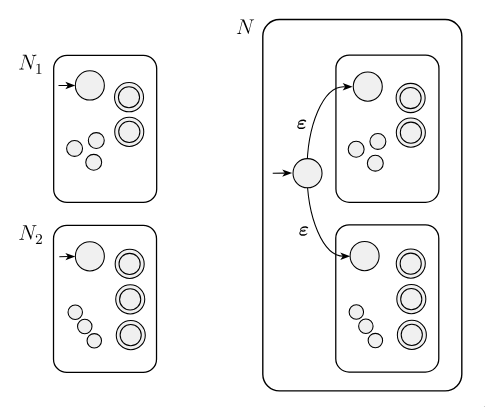
\includegraphics[scale=0.3]{img/2024-12-16-18-34-40.png}
\end{center}

\pf{Dimostrazione formale}{
  Siano $ N_1 = \{Q_1, \Sigma, \delta_1, q_1, F_1\} $ e $ N_2 = \{Q_2, \Sigma, \delta_2, q_2, F_2\} $ NFA che riconoscono rispettivamente $ A_1 $ e $ A_2 $.

  Costruisco un nuovo NFA $ N = \{Q, \Sigma, \delta, q_0, F\} $ per riconoscere $ A_1 \cup A_2 $ in tale modo:
  \begin{enumerate}
    \item $ Q = \{q_0\} \cup Q_1 \cup Q_2 $
    \item $ F = F_1 \cup F_2 $
    \item $ \forall q \in Q. \forall a \in \Sigma. \delta(q, a) = \begin{cases}
    \delta_1(q, a) & q \in Q_1\\
    \delta_2(q, a) & q \in Q_2\\
      \{q_1, q_2\} & q = q_0 \land a = \varepsilon\\
      \emptyset & q = q_0 \land a \neq \varepsilon
    \end{cases} $
  \end{enumerate}

  Quindi per il teorema Basta-Dario e' sVenuto, $ A_1 \cup A_2 $ e' un linguaggio regolare.
}
Ora passiamo alla concatenazione:
\thm{Chiusura dei linguaggi regolari rispetto alla concatenazione}{
  I linguaggi regolari sono chiusi sotto la concatenzazione.

  In altre parole, se $ A_1 $ e $ A_2 $ sono linguaggi regolari, anche $ A_1 \cdot A_2 $ e' regolare.
}
Il punto chiave di questa dimostrazione e' come sapere quando finisce la parola di $ A_1 $ e inizia una stringa di $ A_2 $. Infatti, con i DFA risulta molto piu' complicato, ma dato che possiamo usare i NFA risulta abbastanza banale. Come prima, vogliamo costruire un NFA $ N $ utilizzando altri due NFA $ N_1 $ e $ N_2 $ che riconoscono $ A_1 $ e $ A_2 $. Possiamo fare cio' collegando tutti gli stati finali di $ N_1 $ allo stato iniziale di $ N_2 $, usando transizioni $ \varepsilon $ per accettare tutti i possibili casi. E' possibile, infatti, che una sotto-strina di una parola in $ A_1 $ appartenga anch'essa ad $ A_1 $, quindi senza il nondeterminismo sarebbe impossibile sapere quando passare a $ N_2 $. Se alla fine dell'input $ N_2 $ e' su uno stato finale, allora la parola appartiene a $ A_1 \cdot A_2 $.

\begin{center}
  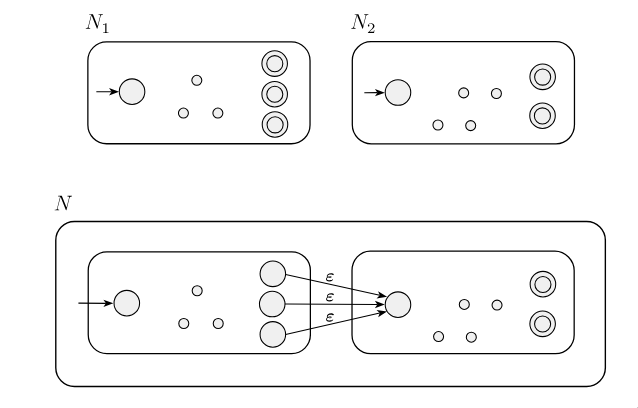
\includegraphics[scale=0.3]{img/2024-12-16-18-35-25.png}
\end{center}

\pf{Dimostrazione formale}{
  Siano $ N_1 = \{Q_1, \Sigma, \delta_1, q_1, F_1\}, N_2 = \{Q_2, \Sigma, \delta_2, q_2, F_2\} $ NFA che riconoscono rispettivamente $ A_1, A_2 $.

  Costruisco il NFA $ N = \{Q, \Sigma, \delta, q_1, F_2\} $ che riconosce $ A_1 \cdot A_2 $ in tale modo:
  \begin{enumerate}
    \item $ Q = Q_1 \cup Q_2 $
    \item $ \forall q \in Q. \forall a \in \Sigma: \delta(q, a) = \begin{cases}
        \delta_1(q, a) & q \in Q_1\setminus F_1\\
      \delta_1(q, a) \cup \{q_2\} & q \in F_1 \land a = \varepsilon\\
      \delta_1(q, a) & q \in F_1 \land a \neq \varepsilon\\
      \delta_2(q, a) & q \in Q_2
    \end{cases} $
  \end{enumerate}

  Sempre per il teorema Basta-Dario e' sVenuto, $ A_1 \cdot A_2 $ e' regolare.
}
Finiamo con la stella di Kleene:
\thm{Chiusura dei linguaggi regolari rispetto alla stella di Kleene}{
  I linguaggi regolari sono chiusi rispetto alla stella di Kleene.

  In altre parole, se $ A_1 $ e' un linguaggio regolare, allora lo e' anche $ A_1^* $.
}
Come nei primi due casi, vogliamo dimostrare per costruzione che esiste un NFA $ N $ che riconosce $ A_1^* $. Considero l' automa $ N_1 $ che riconosce $ A_1 $. Noi vogliamo che $ N $ riconosca una concatenazione di qualunque lunghezza di parole in $ A_1 $, quindi possiamo usare l'idea della dimostrazione precedente e collegare tutti gli stati finali di $ N_1 $ questa volta al proprio stato iniziale, sempre con transizioni $ \varepsilon $. Non possiamo dimenticarci pero' che anche $ \epsilon \in A_1^* $, quindi basta aggiungere un nuovo stato iniziale che sia pure finale e collegarlo al vecchio stato iniziale con un'altra transizione $ \epsilon $.

\begin{center}
  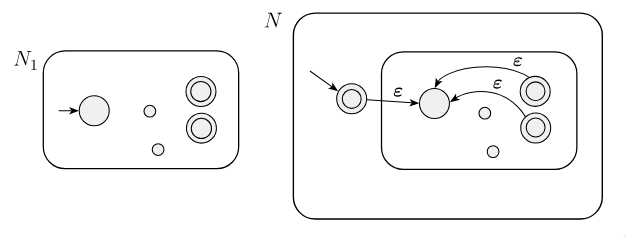
\includegraphics[scale=0.3]{img/2024-12-16-18-36-09.png}
\end{center}

\pf{Dimostrazione formale}{
  Sia $ N_1 = \{Q_1, \Sigma, \delta_1, q_1, F_1\} $ un NFA che riconosce il linguaggio regolare $ A_1 $.

  Costruisco $ N = \{Q, \Sigma, \delta, q_0, F\} $ che riconosce $ A_1^* $ nel seguente modo:
  \begin{enumerate}
    \item $ Q = \{q_0\} \cup Q_1 $
    \item $ F = \{q_0\} \cup F_1 $
    \item $ \forall q \in Q, \forall a \in \Sigma: \delta(q, a) = \begin{cases}
    \delta(q, a) & q \in Q_1 \setminus F_1\\
    \delta(q, a) & q \in F_1 \land a \neq \varepsilon\\
      \delta(q, a) \cup \{q_1\} & q \in F_1 \land a = \varepsilon\\
      \{q_1\} & q = q_0 \land a = \varepsilon\\
      \emptyset & q = q_0 \land a \neq \varepsilon
    \end{cases} $
  \end{enumerate}

  Gia lo sapete cosa ci dicono il Basta e il Darione, $ A_1^* $ e' regolare.
}

TODO: intersezione

\section{Grammatiche regolari}

\dfn{grammatiche regoalre}{
    Una grammatica libero si definisce \textbf{regoalre} sse ogni produzione è della forma $V\to aW$ oppure $V\to a$  dove $V,W\in NT\land a\in T$. Per il simbolo iniziale $S$ è ammessa anche la produzione $S\to \varepsilon$
}

\nt{
    A volte si userà la definizione più lasca che permette produzione $V\to \varepsilon$ anche per nonterminali diversi da $S$ 
}

Di seguito riportati degli esempi
\esempio{
    Sia $G$ la seguente grammatica regolare:
    \[
        \begin{array}{l}
            A \to aA\mid bB\mid bA\\
            B\to a
        \end{array}
    \]

    Si ha che $L(G)= (A|b)^*ba$!!

    Adesso si costruisca un NFA a $G$:
    \begin{center}
        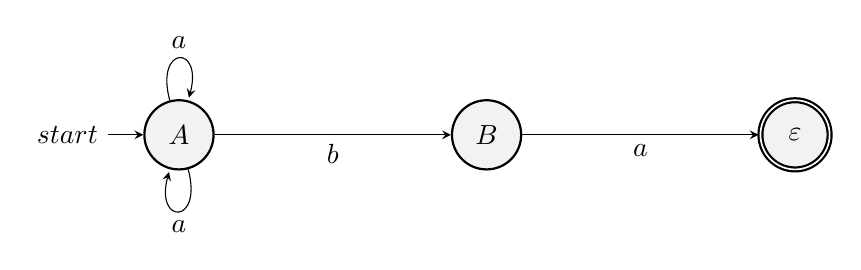
\begin{tikzpicture}
            \node[state, initial] (A) {$A$};
            \node[state] (B) [right=of A] {$B$};
            \node[state, accepting] (C) [right=of B] {$\varepsilon$};

            \path[->]
                (A) edge[loop below] node {$a$} ()
                    edge[loop above] node {$a$} ()
                    edge[below] node {$b$} (B)
                (B) edge[below] node {$a$} (C);
        \end{tikzpicture}
    \end{center}

    si ha che:
    \begin{itemize}
        \item abbiamo associato a ogni nonterminale uno stato dell'NFA
        \item abbiamo aggiunto stato finale $\varepsilon$
    \end{itemize}
}

Esempio 2:
\esempio{
    Sia $G$ la seguente grammatica regolare:
    \[
        \begin{array}{l}
            A\to aA\mid bB \\
            B\to bB\mid aC\mid a\\
            c\to aA \mid bB
        \end{array}
    \]
    l'NFA è:

    \begin{center}
       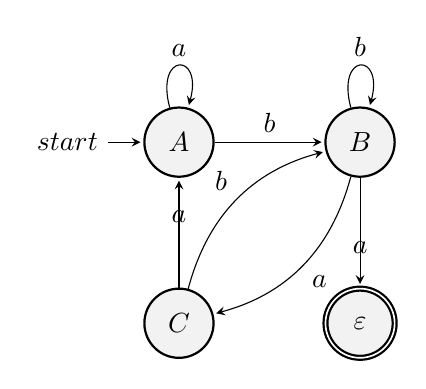
\begin{tikzpicture}[shorten >=1pt, node distance=2.3cm, on grid, auto]
        \node[state, initial] (A) {$A$};
        \node[state] (B) [right=of A] {$B$};
        \node[state] (C) [below=of A] {$C$};
        \node[state, accepting] (D) [below=of B] {$\varepsilon$};

        \path[->]
                (A) edge[loop above] node {$a$} ()
                    edge[above] node {$b$} (B)
                (B) 
                    edge[loop above] node {$b$} ()
                    edge[below] node {$a$} (D)
                    edge[bend left] node[align=left] {$a$} (C)
                (C)
                    edge[above] node {$a$} (A)
                    edge[bend left] node[align=left] {$b$} (B);

    \end{tikzpicture} 
    \end{center}
    
}

\subsection{da grammatiche regolari a NFA equivalenti}
\thm{}{
    Data una grammatica regoalre $G$ si può costruire un NFA $N_G$ equivalente
}
\dimostrazione{
    Sia $G=(NT, T, R, S)$, definiamo inoltre $N_G=(T,Q,\delta, S,\{\varepsilon\})$ come segue:
    \begin{itemize}
        \item $Q=NT\cup \{\varepsilon\}$
        \item $\delta$ definita come segue:
            \begin{itemize}
                \item $(V\to aZ\in R)\implies (Z\in\delta (V,a))$
                \item $(V\to a\in R)\implies (\varepsilon\in\delta (V,a))$
                \item $(V\to \varepsilon\in R)\implies (\epsilon\in\delta (V,\epsilon))$
            \end{itemize}
    \end{itemize}
    Si può dimostrare che
    \[
        S\implies^*_G w \text{ con la grammatica} G \iff (S,w)\vdash_{N_G}^* \text{ con l'automa }N_G
    \]

    non verrà dimostrata quest'ultima parte cazzo
}

\subsection{Da DFA a grammatiche regolari}
\thm{}{
    Da un DFA $M$ possiamo definire una grammatica regolare $G_M$ tale che:
    \[
        L[M] = L(G_M)
    \]
}
\dimostrazione{
    Sia $\mathcal{M} = (\Sigma, Q, \delta, q_0, F)$ il DFA. La grammatica $G_{\mathcal{M}} = (Q, \Sigma, R, q_0)$ ha:
    \begin{itemize}
        \item \textbf{Per non terminali:} gli stati di $\mathcal{M}$.
        \item \textbf{Per terminali:} l'alfabeto di $\mathcal{M}$.
        \item \textbf{Per simbolo iniziale:} lo stato iniziale di $\mathcal{M}$.
        \item \textbf{Per produzioni $R$:}
        \begin{itemize}
            \item Per ogni $\delta(q_i, a) = q_j$, la produzione $q_i \to a q_j \in R$.
            \item Inoltre, se $q_j \in F$, anche $q_i \to a \in R$.
            \item Se $q_0 \in F$, allora $q_0 \to \varepsilon \in R$.
        \end{itemize}
    \end{itemize}

    Versione alternativa che usa la definizione di grammatica regolare più lasca:
    \begin{itemize}
        \item Per ogni $\delta(q_i, a) = q_j$, la produzione $q_i \to a q_j \in R$.
        \item Se $q \in F$, allora $q \to \varepsilon \in R$.
    \end{itemize}

    Si può dimostrare che:
    \[
        w \in L[\mathcal{M}] \iff w \in L(G_{\mathcal{M}})
    \]
}

\esempio{
    Sia $M$:
    \begin{center}
        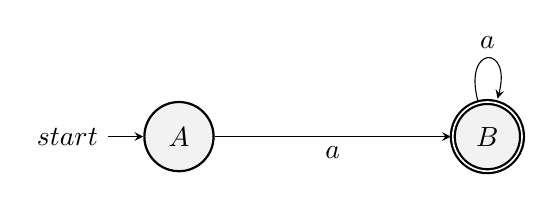
\begin{tikzpicture}
            \node[state, initial] (A) {$A$};
            \node[state, accepting] (B) [right=of A]{$B$};

            \path[->]
                (A) edge[below] node {$a$}(B)
                (B) edge[loop above] node{$a$}(); 
        \end{tikzpicture}
    \end{center}

    Si ha che $aa^*$ è l'espressione regolare che descrive $L[M]$ 

    Secondo la costruzione appena descritta $G_M$ è:
    \[
        \begin{array}{l}
            A\to aB\mid a\\
            B\to aB\mid a
        \end{array}
    \]
    secondo la variante, invece:
    \[
        \begin{array}{l}
            A \to aB\\
            B\to aB\mid \varepsilon
        \end{array}
    \]
}

\esempio{
    sia il seguente automa $M$:
    \begin{center}
        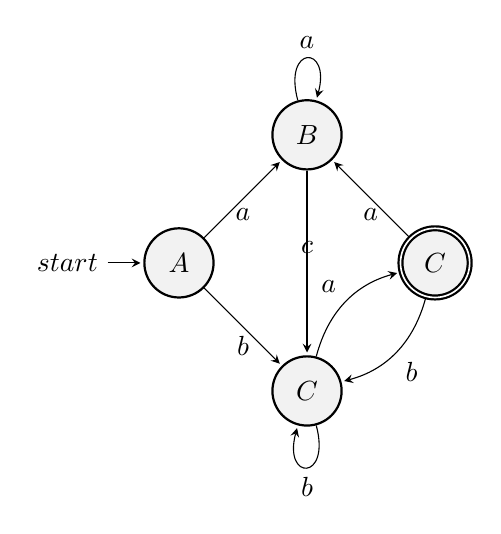
\begin{tikzpicture}[shorten >=1pt, node distance=2.3cm, on grid, auto]
            \node[state, initial] (a) {$A$};
            \node[state] (b) [above right=of a] {$B$};
            \node[state] (c) [below right=of a] {$C$};
            \node[state, accepting] (d) [below right=of b] {$C$};

            \path[->]
                (a) 
                    edge[below] node {$a$} (b)
                    edge[below] node {$b$} (c)
                (b)
                    edge[loop above] node {$a$} ()
                    edge[above] node {$c$} (c)
                (c)
                    edge[loop below] node {$b$} ()
                    edge[bend left] node {$a$} (d)
                (d)
                    edge[below] node {$a$} (b)
                    edge[bend left] node {$b$} (c);
        \end{tikzpicture}
    \end{center}
}

secondo il metodo descritto si ha che $G_M$ è:
\[
    \begin{array}{l}
        A\to aB \mid bC\\
        B\to aB\mid bC\\
        C\to bC\mid aD\mid a\\
        D\to aB\mid bC
    \end{array}
\]
alternativamente:
\[
    A\to aB\mid bC\\
    B\to aBmid bC\\
    C\to bC\mid aD\\
    D\to aB\mid bC\mid \varepsilon
\]
\subsection{Grammatiche regolari ed espressioni regolari}
\thm{}{
    Il linguagio definito da una grammatica regolare $G$ è un linguaggio regolare, cioè è possibile costruire una espressione regolare $S_G$ tale che:
    \[
        L(G)= \mathcal{L}[S_G]
    \] 
}
\pf{sketch della dimostrazione}{
    idea della prova:
    \begin{itemize}
        \item \textbf{caso semplice}: un solo non terminale:
        \[
            A\to aA\mid b\mid \varepsilon
        \]
        è intuitivo vedere che $a^*(b|\varepsilon)$ è la espressione regolare associata
        \item \textbf{caso medio}: due non terminali
        \[
            \begin{array}{l}
                A\to aA\mid bB\mid c\\
                B\to cA\mid aB\mid d
            \end{array}
        \]
        ricaviamo $B$ dalla seconda equzione 
        \[
            B\approx a^*(cA|d) \text{ dove }A\text{ compare nella espressione regolare}
        \]
        ora sostituiamo $B$ nella prima "equazione"
        \[
            A\approx aA\mid ba^*(cA\mid d)\mid c
        \]
        con opportune manipolazioni su espressioni regolari, usando leggi che abbiamo visto, possiamo scrivere
        \[
            A\approx aA\mid ba^*cA\mid ba^*d \mid c
        \]
        e quindi 
        \[
            a\approx (a\mid ba^*c)A \mid ba^*d\mid c
        \]
        ora siamo nella forma "semplice"-

        $A$ ha associata la espressione regolare
        \[
            (a\mid ba^*c)^*(ba^*d\mid c) 
        \]
        \item \textbf{in generale}
        
        \[
        A_1 \simeq a_{11} A_1 \mid \dots \mid a_{1m} A_m \mid b_{1} \mid \dots \mid b_{1p_1}
        \]
        \[
        A_2 \simeq a_{21} A_1 \mid \dots \mid a_{2n} A_n \mid b_{21} \mid \dots \mid b_{2p_2}
        \]
        \[
            \vdots
        \]
        \[
        A_m \simeq a_{m1} A_1 \mid \dots \mid a_{mn} A_n \mid b_{n1} \mid \dots \mid b_{np_n}
        \]

        Si parte con:
        \[
            A_m \simeq S_m \big[ A_1, \dots, A_{n-1} \big]
        \]
        cioè si costruisce una espressione regolare per \( A_m \) che usa \( A_1, \dots, A_{n-1} \).

        Poi si procede sostituendo \( A_n \) (o meglio \( S_n \big[ A_1, \dots, A_{n-1} \big] \)) al posto di \( A_n \) nell'equazione per \( A_{n-1} \), cioè:
        \[
            A_{n-1} \simeq S_{n-1} \big[ A_1, \dots, A_{n-2} \big]
        \]

        e così via fino ad arrivare ad \( A_1 \) (che è il simbolo iniziale).


    \end{itemize}
}

\esempio{
    Sia $G$ la seguente grammatica
    \[
        \begin{array}{l}
            A\to aB\mid \varepsilon\\
            B\to bA\mid \varepsilon
        \end{array}   
    \]
    PEr $B$ la espressione regoalre associata è $(bA\mid \varepsilon)$, sostituisco questa al posto di $B$ nella prima equazione

    \[
        A\approx a (bA\mid \varepsilon)\mid \epsilon
    \]
    manipolo la espressione regoalre
    \[
        A\approx abA\mid a\mid \varepsilon
    \]
    siamo ora nel caso semplice
    \[
        A\approx (ab)^*(a\mid \varepsilon)_{S_G}
    \]
}

\nt{
    la grammatica regolare $G$ con unica prodizone $A\to aA$ definisce il linguaggio vuoto, non $a^*$ quindi $S_G = \varnothing$
}

\subsection{Per riassumere le relazione tra espressioni regolari, linguaggi regolari e automi NFA e DFA}
\vspace{0.5cm}
\begin{center}
    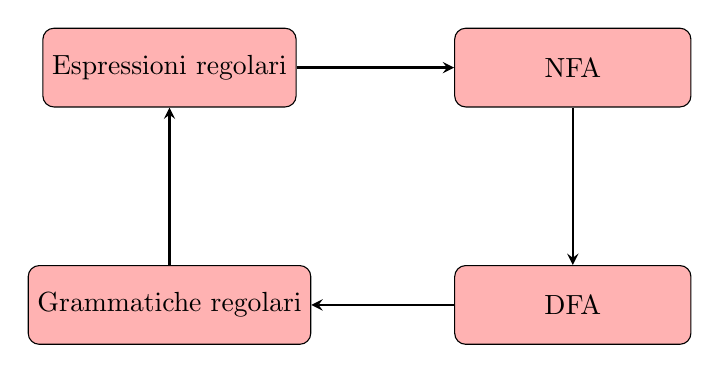
\begin{tikzpicture}[node distance=2cm]
        % Nodes
        \node (regexp) [startstop] {Espressioni regolari};
        \node (nfa) [startstop, right=of regexp] {NFA};
        \node (reggram) [startstop, below=of regexp] {Grammatiche regolari};
        \node (dfa) [startstop, below=of nfa] {DFA};
        
        % Arrows
        \draw [arrow] (regexp) -- (nfa);
        \draw [arrow] (nfa) -- (dfa);
        \draw [arrow] (dfa) -- (reggram);
        \draw [arrow] (reggram) -- (regexp);
    \end{tikzpicture}
\end{center}

\clm{}{}{
    Si osservi che tutti questi formalismi sono equivalenti

    \red{Tutti generano/riconoscono/descrivono la stessa classe di linguaggi, ovvero i linguaggi regolari} 
}

Tuttavia vi è un serio problema, infatti, per costruire uno scanner si parte dalla specifica dei pattern associati alle categorie sintattiche del linguaggio, mediante espressioni regolari. Per poi
\[
    \text{\texttt{regexp}}\to \text{\texttt{NFA}} \to \text{\texttt{DFA}}
\]

ma se l'NFA ha $n$ stati il DFA potrebbe averne al più $2^n$, pertanto serve trovare un DFA equivalente più piccolo possibile
\[
    \min(\text{\texttt{DFA}}) \text{ minimizzato}
\] 

\subsection{minimizzazione}
Alle volte per minimizzare degli automi occorre individuare stati equivalenti nello stesso automa, eliminarli e fonderli insieme costruendo, così, l'automa minimo. Prima della definizione formale occorre definire la seguente notazione:
\dfn{notazione $\hat{\delta}$}{
    Per un DFA $N=(\Sigma, Q,\delta,q_0, F)$ si ha che
    \[
        \begin{array}{ll}
            & \hat{\delta}:Q\times\Sigma^*\to Q \text{ è definita come}\\
            &\hat{\delta}(q,\varepsilon) = q\\
            & \hat{\delta}(q,xa) = \delta(\hat{\delta}(q,x)a)
        \end{array}
    \]

    Si ha quindi 
    \[
        w\in L[N] \iff \hat{\delta}(q_0, w)\in F
    \]
}
\subsubsection{equivalenza/indistinguibilità}
\dfn{stati equivalenti/indistinguibili}{
    due stati si dicono $q_1$ e $q_2$ di un DFA $N$ si definiscono \textbf{equivalenti (o indistinguibili)} se 
    \[
        \forall x\in \Sigma^*\;(\hat{\delta}(q_1,x)\in F\iff \hat{\delta}(q_2, x)\in F)  
    \]
}
Simmetricamente si può definire la non equivalenza
\dfn{
    non equivalenza/indistinguibilità
}{
    due stati $q_1$ e $q_2$ \textbf{non sono equivalenti (o indistinguibili)} se
    \[
        \exists x\in\Sigma^*\;((\hat{\delta}(q_1,x)\in F \land \hat{\delta}(q_2,x)\notin F)\lor (\hat{\delta}(q_1,x)\notin F \land \hat{\delta}(q_2,x)\in F))
    \]
    $q_1$ e $q_2$ pertanto sono distinguibili
}

\nt{
    Una strategia per individuare la distinguibilità tra due stati è cercare di distinguere due stati a partire da $x\in \Sigma^*$ partendo dalla più corta $\varepsilon$
}

Si noti questo esempio
\esempio{
    Sia $N$ il seguente DFA:
    \begin{center}
        \begin{tikzpicture} [node distance=1cm]
            \node[state, initial] (a) {$A$};
            \node[state] (b) [above right=of a] {$B$};
            \node[state] (c) [below right=of a] {$C$};
            \node[state, accepting] (d) [above right=of c] {$D$};

            \path[->]
                (a) 
                    edge node[above] {$a$} (b)
                    edge node[above] {$b$} (c)
                (b)
                    edge[loop above] node {$a$} ()
                    edge node[left] {$b$} (c)
                (c)
                    edge[loop below] node {$b$} ()
                    edge[bend left] node[below] {$a$} (d)
                (d)
                    edge[bend left] node[below] {$b$} (c)
                    edge node[above] {$a$} (b);
        \end{tikzpicture}
    \end{center}

    Inanzi tutto cerco di vedere quali coppie di stati NON sono equivalenti, a partire dalla stringa $\varepsilon$:

    \begin{itemize}
        \item $\varepsilon$ distingue ogni stato in $F$ da ogni stato in $Q\backslash F$, dato ceh $\hat{\delta}(q,\epsilon)=\epsilon$, sicuramente non sono equivalenti:
        \[
            \cancel{(A,D)} \quad \cancel{(B,D)} \quad \cancel{(C,D)}
        \]

        Infatti $A\notin F\land D\in F$, $B\notin F\land D\in F$ e $C\notin F\land D\in F$
        \item adesso si consideri le stringhe di lunghezza q, ovvero $a$ e $b$
        \begin{itemize}
            \item si parti con la lettera $a$:
            \begin{itemize}
                \item $a$ distingue $B$ e $C$ perché
                \[
                    \delta(B,a) = A \text{ e }\delta(C, a) = D
                \]
                E $(B,D)$ l'avevo già cancellata del primo punto
                \item $a$ distingue anche $A$ e $C$ perché
                \[
                    \delta(A,a) = B \text{ e }\delta(C, a) = D
                \]
                E $(B,D)$ l'avevo già cancellata del primo punto
            \end{itemize}
            \item $b$ non permette di fare ulteriori distinzioni
        \end{itemize}
        \item procedo con le stringhe di lunghezza lunghe 2, ma non riesco a fare nessuna ulteriore distinzione. quindi ho finito
    \end{itemize}

    Non sono riuscito a distinguere solo $A$ e $B$, quindi sono equivalenti e li fondo. Il nostro automa finale sarà

    \begin{center}
        \begin{tikzpicture}[node distance=1cm]
            \node[state, initial] (ab) {$A,B$};
            \node[state] (c) [right=of ab] {$C$};
            \node[state, accepting] (d) [right=of d] {$D$};

            \path[->]
                (ab)
                    edge[loop above] node {$a$} ()
                    edge node[above] {$b$} (c)
                (c)
                    edge[loop above] node {$b$} ()
                    edge[bend left] node[above] {$a$} (d)
                (d)
                    edge[bend left] node[above] {$b$} (c)
                    edge[bend left] node[below] {$a$} (ab);
        \end{tikzpicture}
    \end{center}
}

\subsubsection{Famiglia di relazioni}
\dfn{famiglia di relazioni}{
    Dato un DFA $M=(\Sigma, Q, delta, q_0, F)$, defininiamo una famiglia relazione $\sim_i \subseteq Q\times Q$ nel seguente modo:
    \begin{itemize}
        \item $\sim_0 = F\times F\cup (Q\setminus F)\times (Q\setminus F)$ 
        
        ovvero stati che non possono essere distinti da $\varepsilon$
        \item $q_1 \sim_{i+1} q_2 \iff \forall a\in \Sigma\quad \delta(q_1, a)\sim_i\delta(q_2, a)$
        
        ovvero $q_1$ e $q_2$ sono in relazione $\sim,_{i+1}$ se $\forall x \in \Sigma^*$ cin $|x|\leq i+1$
        
        \[
            \hat{\delta}(q_1, x)\in F \iff \hat{\delta}(q_2, x)\in F
        \]
    \end{itemize}
}

\nt{
    Si osservi che:
    \begin{itemize}
        \item La relazione $Id =\{(q,q)\mid q\in Q\}$ è tale che $Id\subseteq \sim_i \forall i$. Si ha in fatti che uno stato è sempre equivalente a se stesso 
        \item $\sim_i$ è una relazione d'equivalenza $\forall i$
        \item \begin{itemize}
                \item $\sim_0$ ha solo 2 classi d'equivalenza, ovvero $F$ e $Q\setminus F$
                \item Per $\sim_i$, riflessività e simmetria sono ovvie, mentre la transitività è meno banale:
                \[
                    q_1 \sim_i q_2 \text{ e }q_2\sim_i q_3 \implies q_1 \sim_i q_3
                \]
            \end{itemize}
        \item Ad ogni passo, rimuovo qualche coppia! \\
            Si verifica che:
            \[
                \sim_0 \supseteq \sim_1 \supseteq \sim_2 \supseteq \sim_3 \supseteq \dots
            \]
            Ossia una \textbf{catena decrescente} (o non crescente) di relazioni di equivalenza.
    
        \item Se esiste un \(K\) tale che \(\sim_K = \sim_{K+1}\), allora per ogni \(j > K\) vale che \(\sim_j = \sim_K\). \\
            In altre parole: Non appena la relazione non viene modificata in un passo, ho trovato la soluzione
    
        \item Un tale \(K\) esiste sicuramente ed è minore di:
            \[
            |\sim_0| = |F \times F| + |(Q \setminus F) \times (Q \setminus F)| = |F|^2 + |Q \setminus F|^2
            \]
            Questo perché, nella peggiore delle ipotesi, ad ogni passo iterativo si rimuove solo una (o al massimo due) coppia.
        
            In realtà si può dimostrare che \(K < |Q| - 1\), poiché \(|Q|\) è la lunghezza del massimo cammino aciclico. Infatti, negli esempi che abbiamo visto, ho considerato solo stringhe che non portavano a cicli.
    
    \end{itemize}
}

\teorema{
    Siano $\sim_2$, $\sim_1$ e $\sim_3$ le relazioni d'equivalenza mostrate poc'anzi si ha che
    \[
        \sim_2=\sim_1 \implies \sim_3=\sim_2
    \]
}
\pf{Dimostrazione con un esempio}{
    Supponiamo, per assurdo, che \(r_2 = r_1\) ma che \(r_3 \neq r_2\), cioè esistano \(A, B\) tali che:
    \[
    A \sim_2 B \quad \text{ma} \quad A \not\sim_3 B,
    \]
    ossia:
    \[
    \sim_3 \subset r_2 = r_1.
    \]

    Allora, poiché \(A \not\sim_3 B\), deve essere:
    \[
    A \xrightarrow{a_1} A_1 \xrightarrow{a_2} A_2 \xrightarrow{a_3} A_3
    \]
    \[
    B \xrightarrow{a_1} B_1 \xrightarrow{a_2} B_2 \xrightarrow{a_3} B_3
    \]
    con \(A_3 \in F\) e \(B_3 \notin F\) (ovviamente).

    Ma allora \(A_1 \not\sim_2 B_1\) e poiché \(r_2 = r_1\), deve essere:
    \[
    A_1 \not\sim_1 B_1.
    \]
    Ma allora:
    \[
    A_1 \xrightarrow{b} A_u \quad B_1 \xrightarrow{b} B_u
    \]
    con \(A_u \in F\) e \(B_u \notin F\) (ovviamente).

    Ma allora \(A \not\sim_2 B\) perché:
    \[
    A \xrightarrow{a_1} A_1 \xrightarrow{b} A_u \quad B \xrightarrow{a_1} B_1 \xrightarrow{b} B_u,
    \]
    contraddicendo l'ipotesi iniziale.

    \[
    \implies \text{non è possibile che } r_1 = r_2 \text{ e } r_3 \subset r_2.
    \]

    \bigskip

    Quindi, se \(\sim_{K+1} = \sim_K\), allora per ogni \(j > K\) vale \(\sim_j = \sim_K\)
}

\esempio{
    Proviamo a minimizzare il DFA seguente:
    \begin{center}
        \begin{tikzpicture}[shorten >=1pt, node distance=2cm, on grid, auto]
           \node[state, initial] (A)   {A}; 
           \node[state] (B) [right=of A] {B}; 
           \node[state, accepting] (C) [below=of A] {C}; 
           \node[state, accepting] (D) [right=of C] {D};
           \node[state, accepting] (E) [below=of C] {E}; 
           \node[state] (F) [right=of E] {F};
            
            \path[->] 
            (A) edge [bend left] node[above] {0} (B)
                edge node {1} (C)
            (B) edge [bend left] node[above] {0} (A)
                edge node {1} (D)
            (C) edge node[above left] {1} (F)
                edge node[left] {0} (E)
            (D) edge node[above right] {0} (E)
                edge node[right] {1} (F)
            (E) edge [loop below] node {0} ()
                edge node {1} (F)
            (F) edge [loop below] node {0,1} ();
        \end{tikzpicture}
    \end{center}
    Costruiamo ora l'insieme \(\sim_0\) come per definizione:
    \[
        \sim_0 = \{(A,A), (B,B), (A,F), (B,A), (B,F), (F,F), (F,A), (F,B)\} 
    \]
    \[
        \cup
    \]
    \[
        \{(C,C), (C,D), (C,E), (D,C), (D,D), (D,E), (E,C), (E,D), (E,E)\}.
    \]

    Procediamo ora per costruire l'insieme \(\sim_1\). Per velocizzare controlliamo solo le coppie in \(\sim_0\) e ovviamente non quelle identiche (tipo \((A,A)\)). Per ora consideriamo solo stringhe di lunghezza \(1\) ("0" e "1"). Otteniamo:
    \[
    \sim_1 = \{(A,A), (A,B), (B,B), (A,F), (B,A), (B,F), (F,F)\} \cup
    \]
    \[
    \{(C,C), (C,D), (C,E), (D,C), (D,D), (D,E), (E,C), (E,D), (E,E)\}.
    \]

    Si ha che \(\sim_2 = \sim_1\), quindi possiamo terminare e ridisegnare il DFA. Gli stati equivalenti sono quindi quelli che non compaiono nelle coppie \((A,B), (F)\), \((C,D,E)\). Otteniamo quindi:

    \begin{center}
    \begin{tikzpicture}[shorten >=1pt, node distance=2cm, on grid, auto]
    \node[state, initial] (AB)   {A, B}; 
    \node[state] (CDE) [right=of AB] {C, D, E}; 
    \node[state, accepting] (F) [right=of CDE] {F};
        
        \path[->] 
        (AB) edge [loop above] node {0} ()
            edge node {1} (CDE)
        (CDE) edge [loop above] node {0} ()
            edge node {1} (F)
        (F) edge [loop above] node {0,1} ();
    \end{tikzpicture}
    \end{center}

    È semplice anche dire che la regex associata è \(0^*10^*\). Inoltre, lo stato \(F\) rappresenta uno stato di errore a cui si arriva con stringhe del tipo \(0^*10^*10^+\).
}

\subsubsection{tabella d'equivalenza}

Le tabella di equivalenza sono un modo per memorizzare l'equivalenza ,di modo, da costruire un algoritmo per la minimizzazione poi, l'idea è la seguente 

\begin{itemize}
    \item \textbf{Tabella con solo coppie "vere".}
    \item Al round 0 dell'algoritmo iterativo, metto una marca \( X_0 \) per indicare che la coppia è distinta:

          \((\text{finale}, \text{non finale})\) oppure \((\text{non finale}, \text{finale})\).
    \item Al round 1, metto la marca \( X_1 \) per distinguere le coppie \((q_1, q_2)\) non ancora marcate che, per qualche \( a \in \Sigma \), 
          hanno \((\delta(q_1, a), \delta(q_2, a))\) già marcata.
    \item Al round 2, metto la marca \( X_2 \) e così via per le coppie successive.
    \item \textbf{Condizione di arresto:} se non riesco a mettere nessuna nuova marca in un round, l'algoritmo termina.
\end{itemize}
\esempio{
    Prendiamo in esame il DFA dell'esempio precedente

    Prima di tutto costruiamo una tabella con solo delle coppie che non sono identiche per far ciò la costruiamo a scaletta. Si ha che:

    \[
        \begin{array}{|c|c|c|c|c|c|c|}
            \hline
            & A & B & C & D & E \\ \hline
            B  & X_0 &    &    &    &    \\ \hline
            C  & X_0 & X_0 &    &    &    \\ \hline
            D  & X_0 & X_0 & X_0 &    &    \\ \hline
            E  & X_0 & X_0 & X_0 & X_0 &    \\ \hline
            F  & X_1 & X_1 & X_0 & X_0 & X_0 \\ \hline
        \end{array}
    \]
}

Per calcolarla è possibile utilizzare il seguente algoritmo
\begin{algorithm}
    \caption{Costruzione di una tabella d'equivalenza}
    \KwIn{DFA N}
    \KwOut{tabella d'equivalenza}

    Sia $T^{n\times n}$ dove $T$ è il numero di stati in $n$\;
    marca $x_0$ ogni coppia $(q_1, q_2)$ tale che $q_1\in F$ e $q_2\in Q\setminus F$ o viceversa\;
    $b \gets true$\;
    $i\gets 1$\;
    \While{b}{
        $b\gets false$\;
        \ForEach{$(q_1, q_2)$ non marcata}{
            \If{$\exists a\in \Sigma$ con $(\delta(q_1,a),\delta(q_2,a))$ già marcate}{
                marca $(q_1, q_2)$ con $x_i$\;
                $b\gets true$\;
            }
        $i\gets i+1$\;
        }
    }
\end{algorithm}

\thm{}{
    Dato un DFA $M=(\Sigma, Q, \delta, q_0, F)$  l’algoritmo della tabella a scala termina, inoltre due stati $p$ e $q$ sono distinguibili se e solo se la casella $(p, q)$ (o la casella $(q, p))$ e marcata 
}
\dimostrazione{
    Procedo a dimostrare le due parti 
    \begin{itemize}
        \item Poiché abbiamo visto che $\exists k.\sim_k=\sim_{k+1}$ e quando l'algoritmo iterativo termina entro $k$ iterazioni
        \item procedo a dimostrare la distinguibilità:
        \begin{itemize}
            \item $\Rightarrow$
            Se $p$ e $q$ sono distinguibili, allora $\exists x\in \Sigma^*.\hat{\delta}(p,x)\in F$ e $\hat{\delta}(q,x \notin F)$ (o viceversa).

            Se prendo $k=|x|$, allora di sicuro $(p,q)\notin \sim_k$ cioè $(p,q)$ viene marcata entro il round $k$
            \item $\Leftarrow$
            
            Se $(p,q)$ sono marcati, allora sicuramente $(p,q)$ sono distinguibili:

            occorre prendere la catena di coppie che portano ad una coppia non presente in $\sim_0$. ad esempio
            \[
                (p,q)\to (p',q')\to (p'', q'')
            \]
            Allora $ab$ è la stringa che distingua $p$ e $q$
        \end{itemize} 
    \end{itemize}
}

\subsection{automa minimo}
\dfn{Automa minimo}{
    Dato un DFA $M = (\Sigma, Q, \delta, q_0, F)$, l'automa minimo equivalente $M_{min} = (\Sigma, Q_{min}, \delta_{min}, [q_0], F_{min})$ è dato da:
    \begin{itemize}
        \item $Q_{min} = \{[q]\mid q\in Q\}$ con $[q]=[q'\in Q\mid q\sim q']$
        
        Gli stati di $M_{min}$ sono classi di equivalenza di stati di $M$
        \item $\delta_{min}([q],a) = [\delta(q,a)]$
        \item $F_{min} = \{[q]\mid q\in F\}$
    \end{itemize}
}

\nt{
    non esistono 2 stati distinti in $M_{min}$ che siano tra loro equivalenti:
    \[
        [q]\neq[q'] \implies q \cancel{\sim} q'    
    \]
}

Adesso estendiamo la notazione di $\hat{\delta}$ per i DFA $M_{min}$
\[
    \begin{array}{l}
        \hat{\delta}_{min} : Q_{min}\times\Sigma^* \to Q_{min}\\
        \hat{\delta}_{min}([q],\varepsilon) = [q]\\
        \hat{\delta}_{min}([q], xa) =\hat{\delta}_{min}(\hat{\delta}_{min}([q],x),a)\\
        w\in L [M_{min}]\iff\hat{\delta}_{min}([q_0],w)\in F_{min}
    \end{array}
\]

\thm{Morbidelli - Morigi (innamorato italiano, innamorata giapponese)}{
    Dato un DFA $M=(\Sigma, Q, \delta, q_0, F)$ l'automa $M_{min} = (\Sigma, Q_{min}, \delta_{min}, [q_0], F_{min})$ riconosce lo stesso linguaggio di $M$, ed ha il minimo numero di stati tra tutti gli automi deterministici per questo linguaggio
}

\dimostrazione{
    Dimostriamo per gradi:
    \begin{itemize}
        \item dimostro che $M_{min}$ è ben definito, cioè $\delta_{min}$ non dipende dallo specifico stato scelto per rappresentare la classe di equivalenza.
        
        Si ha se $q\sim q'$, allora:
        \begin{itemize}
            \item $[q] = [q']$
            \item $\delta_{min}([q], a)=[\delta]=[\delta(q',a)] = \delta_{min}([q',a])$
        \end{itemize}

        Se non fosse vero allora $\delta(q,a)$ e $\delta(q', a)$ sarebbero distinguibili, quindi pure $q$ e $q'$
        \item Per dimostrare che $L[M]=L[M_{min}]$, dimostrare che 
        \[
            \hat{\delta} (q_0, w) = r \iff \hat{\delta}([q_0], w) = [r]
        \]
        ovvero che
        \[
            \hat{\delta}([q_0], w) = [\hat{\delta}, w]
        \]
        si fa la dimostrazione per induzione su $|w|$
        \begin{itemize}
            \item Caso base: $|w| = 0$ cioè $e=\varepsilon$
            \[
                \hat{\delta}(q_0,\varepsilon) = q_0 \quad \hat{\delta}([q_0], \epsilon) =[q_0]  =[\hat{\delta}(q_0, \epsilon)]
            \]
            Dimostrato
            \item Passo induttivo: $w = xa$
            \[
                \hat{\delta}(q_0, xa) = \delta(\hat{\delta}(q_0, x),a)
            \]
            e, per definizione di $\hat{\delta}_{min}$
            \[
                \hat{\delta} ( [q_0], xa) = \delta_{min}( \hat{\delta}([q_0],x),a) 
            \]
            Per ipotesi induttiva
            \[
                \delta_{min}( \hat{\delta}([q_0],x),a) = \delta_{min}([\hat{\delta}(q_0, x)],a)
            \]
            per definizione di $\delta_{min}$
            \[
                \delta_{min}([\hat{\delta}(q_0, x)],a) = [\delta(\hat{\delta}(q_0,x),a)]
            \]
            per definizione di $\hat{\delta}$
            \[
                [\delta(\hat{\delta}(q_0,x),a)] = [\hat{\delta}(q_0, xa)]
            \]
            Quindi
            \[
                w\in L[M]\iff \hat{\delta}(q_0,w) = r\in F \iff \hat{\delta}_{min}([q_0], w) = [r]\in F_{min} \iff w\in L[M_{min}]
            \]
        \end{itemize}
        \item rimane da dimostrare che è minimo, ovvero che un qualunque altro automa deterministico $N$ non puà avere meno stati
        Supponiamo esista un DFA $N$ tale che $L[N]=L[M_{min}]$, ma con un numero di stati inferiore a quelli di $M_{min}$
        \begin{itemize}
            \item Gli stati iniziali di \( N \) e \( M_{\text{min}} \) devono essere equivalenti (nell'automa \( N \cup M_{\text{min}} \)), poiché \( L[N] = L[M_{\text{min}}] \).
                  \begin{itemize}
                      \item Infatti, si suppone che \( N \) e \( M_{\text{min}} \) abbiano lo stesso linguaggio.
                  \end{itemize}
        
            \item Se più \( q \in M_{\text{min}} \) e \( q' \in N \) sono equivalenti, nell'automa \( N \cup M_{\text{min}} \), allora sono equivalenti anche i loro successori per ogni \( a \in \Sigma \).
        
            \item \( N \) non ha stati inaccessibili dal suo iniziale (altrimenti si potrebbe costruire un automa \( N' \) con ancora meno stati). 
                  \begin{itemize}
                      \item \( M_{\text{min}} \) non ha stati inaccessibili per costruzione.
                  \end{itemize}
                  Di conseguenza, ogni stato di \( M_{\text{min}} \) è equivalente ad almeno uno stato di \( N \) (per il punto precedente).
        
            \item Poiché \( N \) ha meno stati di \( M_{\text{min}} \), due stati \( p \) e \( p' \) di \( M_{\text{min}} \) devono essere equivalenti ad uno stesso stato \( q \) di \( N \). 
                  \begin{itemize}
                      \item Ma la relazione di equivalenza \( \sim \) è transitiva, quindi \( p \sim p' \) e dunque \( p \) e \( p' \) devono essere equivalenti!
                      \item Ma questo è impossibile!
                  \end{itemize}
                  Per costruzione di \( M_{\text{min}} \), non ci sono due stati diversi in \( M_{\text{min}} \) equivalenti tra loro.
        \end{itemize}
    \end{itemize}
}

\section{Espressivita' dei linguaggi regolari e pumping lemma}
Finora abbiamo parlato solo di linguaggi regolari, senza dimostrare l'esistenza di altri tipi di linguaggi piu' espressivi. In questa sezione, faremo vedere che esistono linguaggi che non possono essere riconosciuti da automi finiti.

Prendiamo come esempio il linguaggio $ B = \{0^n 1^n \mid n \geq 0\} $. Per costruire un automa che lo riconosca, dobbiamo ricordarci il numoro di $ 0 $ inseriti all'inizio per controllare che il numero di $ 1 $ sia uguale. Ma, dato che il valore di $ n $ non ha un limite superiore, dobbiamo rappresentare un numero infinito di valori di $ n $ con un numero finito di stati, che dimostreremo essere impossibile in questo caso.

Potrebbe sembrare che qualunque linguaggio simile a $ B $ con $ n $ illimitato sia non regolare, ma questo non e' corretto. Anche se a prima apparenza puo' sembrare che un linguaggio necessiti di memoria infinita, ci possono essere modi intelligenti per circonvenire questa apparente necessita'. Prendiamo, ad esempio, il linguaggio $ C = \{w \mid w \text{ha un ugual numero di sottostringhe 01 e 10}\} $, si puo' dimostrare che questo linguaggio sia regolare! Quindi la nostra intuizione puo' spesso sbagliare, vediamo ora un modo per dimostrare per certo che certi linguaggi non sono regolari:

\subsection{Pumping lemma}
Il pumping lemma e' un teorema che attribuisce una proprieta' speciale a tutti i linguaggi regolari. Se un linguaggio non ha questa proprieta', allora sappiamo per certo che non e' regolare. In breve, la proprieta' dice che ogni stringa di un linguaggio regolare puo' essere "pompata" se e' almeno lunga quanto una specifica lunghezza chiamata \textbf{lunghezza di pompaggio HHahaHAahaha}. Ovvero, ognuna di queste stringhe ha una sezione che puo' essere concatenata a se stessa un numero illimitato di volte e la stringa risultante fa sempre parte dello stesso linguaggio. 

\thm{Pumping lemma}{
  Sia $ A $ un linguaggio regolare, allora $ \exists p $ tale che $ \forall s \in A. s \geq p $, $ s $ puo' essere suddivisa in tre parti $ s = xyz $ tali che:
  \begin{enumerate}
    \item $ \forall i \geq 0. xy^iz \in A $
    \item $ |y| > 0 $
    \item $ |xy| \leq p $
  \end{enumerate}
}
In questa formalizzazione, $ y $ e' la parte della stringa che puo' essere ripetuta (condizione 1), che deve essere non nulla per non rendere trivialmente vero il teorema (condizione 2). La terza condizione sara' utile per dimostrare che certi linguaggi non sono regolari, e ci dira' che prendiamo la \textbf{prima} porzione della stringa che puo' essere ripetuta. Vediamo perche':

\subsubsection{Dimostrazione}
Prima della dimostrazione formale, proviamo a capire l'idea di base. Sia $ M = (Q, \Sigma, \delta, q_1, F) $ un DFA che riconosce $ A $. Poniamo che la lunghezza di pompaggio sia uguale al numero di stati di $ M $ ($ p = |Q| $). Se in $ A $ non ci sono stringhe di tale lunghezza, allora il teorema e' ovviamente vero perche' vale per tutte le zero stringhe a cui puo' essere applicato.

Altrimenti, $ \exists w \in A. |w| = n \geq p $ che viene accettato da $ M $ passando da una serie di stati $ q_1, q_3, q_{20}, q_9, ..., q_{13} $ (dove $ q_1 $ e' lo stato iniziale e $ q_{13} \in F $), che avra' lunghezza uguale a $ n+1 $. Dato che $ n \geq p $, siamo sicuri che $ n+1 > p $, quindi ci sono piu' stati nella sequenza di quanti stati distinti esistano. Allora, ci deve essere per forza uno stato che si ripete (per il \textbf{pigeonhole principle}):
\[
s = \mid_{q_1} s_1  \mid_{q_3} s_2 \mid_{q_{20}} s_3 \mid_{q_9} s_4 \mid_{q_{17}} s_5 \mid_{q_9} s_6 \mid_{q_6} ... \mid_{q_{35}} s_n \mid_{q_{13}}
\]
in questo caso, lo stato $ q_9 $ e' il primo che si ripete. Possiamo ora dividere $ s $ in tre parti $ x, y $ e $ z $: $ x $ e' la parte di $ s $ prima di di $ q_9 $, $ y $ e' la parte fra le due ripetizioni di $ q_9 $ e $ z $ e' la parte rimanente. 

\begin{center}
  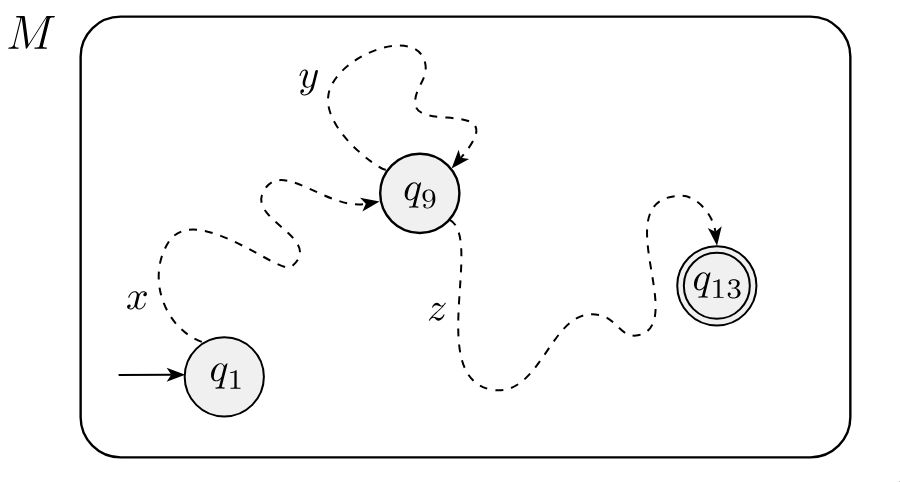
\includegraphics[scale=0.3]{img/2024-12-08-17-37-33.png}
\end{center}

Vediamo perche' questa suddivisione rispetta le tre condizioni. Consideriamo l'input $ xyyz $ passato a $ M $: $ x $ ci porta da $ q_1  $ a $ q_9 $, la prima $ y $ ci porta da $ q_9 $ a $ q_9 $, anche la seconda ci porta da $ q_9 $ a $ q_9 $, infine $ z $ ci porta da $ q_9 $ a $ q_{13} $ (lo stato finale). Quindi $ xyyz $ e' accettato da $ M $, ma anche $ xy^iz $ per lo stesso motivo. Nel caso $ xy^0z $ vediamo che viene riconosciuto anche lui, quidi la prima condizione e' verificata. Dato che $ y $ e' la parte della stringa che ci porta da $ q_9 $ a $ q_9 $, deve essere per forza non nulla perche $ M $ e' deterministico. Infine, la terza condizione e' rispettata dato che, per la \textbf{pigeonhole principle} la prima ripetizione deve avvenire per forza entro i primi $ p+1 $ stati, quindi $ |xy| \leq p $.

\pf{Dimostrazione formale}{
  Sia $ M = (Q, \Sigma, \delta, q_1, F) $ un DFA che riconosce il linguaggio regolare $ A $ e $ p = |Q| $.

  Sia $ s = s_1s_2...s_n $ una stringa in $ A $ tale che $ |s| = n \geq p $ e siano $ r_1, r_2, ..., r_{n+1} $ la sequenza di stati che attraversa $ M $ quando viene dato $ s $ come input, quindi $ r_{i+1} = \delta(r_i, s_i) $. Dato che $ n+1 \geq p+1 $, per il pigeonhole principle fra i primi $ p+1 $ stati ce ne deve essere uno che si ripete. Chimiamo $ r_j $ il primo e $ r_l $ la ripetizione, quindi abbiamo che $ l \leq p+1 $. 

  Ora siano $ x = s_1 ... s_{j-1} $, $ y = s_j ... s_{l-1} $ e $ z = s_l ... s_{n} $. Dato che $ x $ porta $ M $ da $ r_1 $ a $ r_j $, $ y $ porta da $ r_j $ a $ r_l $ e $ z $ porta da $ r_l $ a $ r_{n+1} $ e siccome $ r_j $ e $ r_l $ sono lo stesso stato, $ M $ deve accettare $ xy^iz $ $ \forall i \geq 0 $. Siccome $ j \neq l $, $ |y| > 0 $; e $ l \leq p+1 $, quindi $ |xy| \leq p $. Abbiamo quindi soddisfatto tutte le condizioni del pumping lemma.
}

\subsubsection{Utilizzo ed esempi}
Per dimostrare che $ B $ non e' un linguaggio regolare, prima assumiamo che $ B $ sia regolare e poi dimostriamo che non vale la proprieta' $ P $ del pumping lemma:
\[
\lnot P \implies B \text{ non e' regolare}
\]
Dato che porprio per il lemma, $ B $ e' regolare $ \implies P $. Quindi, bisogna assumere che $ p $ sia la lunghezza garantita dal pumping lemma e prendere una stringa $ s \in B. |s| \geq p $ tale che noi sappiamo che $ z $ non puo' essere pompata. Dimostriamo questo mostrando che per qualunque suddivisione $ xyz $ che rispetti le ultime due condizioni, la prima condizione non vale mai. Solitamente possiamo raggruppare i tipi di suddivisione in diverse categorie che possono essere analizzate individualmente, in modo da non dover controllare davvero ogni suddivisione. Trovando $ s $, abbiamo dimostrato $ \lnot P $ e quindi che $ B $ non e' regolare. 

Per trovare $ s $, solitamente ci vuole un po' di creativita. Bisogna provare a trovare una stringa che raccolga l'"essenza" dell'irregolarita' del linguaggio, vediamo un paio di esempi per chiarire:
\ex{}{
  $ B = \{0^n 1^n \mid n \geq 0\} $
}
\ex{}{
  $ C = \{w \mid w \text{ ha lo stesso numero di 0 e 1}\} $
}
\ex{}{
  $ F = \{ww \mid w \in \{0, 1\}^*\} $
}
TODO: fai esercizi (che sono risolti sul libro)

\chapter{Linguaggi liberi nondeterministici}
Fino ad ora abbiamo studiato due modi equivalenti per descrivere linguaggi: gli \textbf{automi finiti} e le \textbf{espressioni regolari}. Abbiamo anche visto le limitazioni di questi metodi, che non riescono ad accettare linguaggi, anche alcuni semplici come $ \{0^n 1^n \mid n \geq 0\} $. 

Per espandere la quantita' di linguaggi che possiamo studiare, introduciamo le cosidette \textbf{grammatiche libere (dal contesto)}, un metodo piu' potente che permette di descrivere certe proprieta' di linguaggi che hanno una struttura ricorsiva. Inizialmente queste grammatiche sono state studiate per analizzare linguaggi umani, ma piu' recentemente hanno visto svariate applicazioni, come nel caso dei \textbf{parser}, utilizzati dalla maggior parte di compilatori e interpreti per estrarre il significato dal codice. 

L'insieme dei linguaggi che possono essere riconosciute da grammatiche libere sono i \textbf{linguaggi liberi (dal contesto)}, che includono propriamente i linguaggi regolari. Per riconoscere tali linguaggi, introdurremo un nuovo tipo di automa: l'\textbf{automa a pila} (PDA - pushdown automata).

\section{Grammatiche libere}
Per qualche motivo, le grammatiche libere le abbiamo viste all'inizio, io le metterei qua ma va beh andate qui per capire cosa sono: \ref{dfn: gramLib}

\subsection{Semplificazione e forme normali}
Questa roba qua invece e' stata messa nei linguaggi liberi deterministici, secondo me ha piu' senzo metterla qua' o fare proprio un capitolo solo sulle grammatiche: \ref{semplificazioneGram}

\section{PDA}
In che modo possiamo modificare gli automi visti fin'ora (DFA/NFA) per far si che riescano a riconoscere linguaggi non-regonalari?

Vediamo ad esempio il linguaggio $ L = \{ww^R \mid w \in \{a, b\}^*\} $. Si puo' dimostrare (fallo per esercizio) che non e' un linguaggio regolare, dato che per riconoscerlo si dovrebbe \textbf{memorizzare} tutta la prima parte della parola palindroma (la cui lunghezza non e' limitata). Quindi serve una forma di memoria ausiliaria, che nei PDA e' imlementata con una \textbf{pila} con memoria illimitata. 

Essendo una pila (LIFO), ci sono certe restrizioni per come puo' essere gestita la memoria:
\begin{itemize}
  \item Si puo' leggere solo il primo elemento in cima alla pila (top)
  \item Si puo' rimuovere solo l'elemento top
  \item Si puo' aggiungere elementi solo in cima alla pila (in modo che diventino il nuovo top)
\end{itemize}

I PDA possono essere \textit{nondeterministici}, e come tali hanno una potenza espressiva maggiore rispetto ai PDA deterministici (DPDA). Dimostreremo alla fine della sezione che i PDA (nondeterministici) hanno lo stesso potere espressivo delle grammatiche libere.

\subsection{Definizione formale}
La definizione formale di un PDA e' simile a quella dei NFA, con l'aggiunta della presenza della pila. Questa pila contiene simboli di un alfabeto che puo' essere diverso rispetto a quello di input, quindi dobbiamo definire sia un alfabeto $ \Sigma $ per l'input, sia l'alfabeto $ \Gamma $ per la pila. L'operazione di transizione, che ci dice come si comporta l'automa, ha come dominio $ Q \times \Sigma_\epsilon \times \Gamma $ (dove $ \Sigma_\epsilon = \Sigma \cup \{\epsilon\} $), quindi la mossa del PDA e' determinata dallo stato corrente, dal carattere in input e dal carattere in cima alla pila. Di questi, il secondo puo' essere anche $ \epsilon $, quindi la macchina puo' fare una mossa senza leggere l'input, ma il simbolo in cima alla stack viene sempre letto (e consumato). 

Dato un input, l'automa puo' spostarsi su un nuovo stato e aggiungere un numero arbitrario di elementi alla pila (anche nessuno). Inoltre, dato che il nondeterminismo ha come conseguenza la possibilita' di avere diverse transizioni possibili dato lo stesso input, dobbiamo considerare come codominio l'insieme di tutti i possibili insiemi che hanno come elementi coppie del tipo $ Q \times \Gamma^* $, ovvero l'insieme potenza $ \mathcal{P}(Q \times \Gamma^*) $. 

\dfn{PDA}{
  Un automa a pila nondeterministico e' una 7-pla $ (Q, \Sigma, \Gamma, \delta, q_0, \bot, F) $ dove:
  \begin{itemize}
    \item $ Q $ e' un insieme finito di stati
    \item $ \Sigma $ e' un alfabeto di input finito
    \item $ \Gamma $ e' un alfabeto per la pila finito
    \item $ \delta: Q \times \Sigma_\epsilon \times \Gamma \to Q \times \Gamma^* $ e' la funzione di transizione
    \item $ q_0 $ e' lo stato iniziale
    \item $ \bot \in \Gamma $ e' il primo simbolo sulla pila
    \item $ F \subset Q $ e' l'insieme degli stati finali
  \end{itemize}

}

\subsection{Transizioni}

A ogni passo di computazione, possiamo attribuire a un PDA una \textbf{descrizione instantanea} (o configurazione) che ci dice lo stato corrente $ q \in Q $, l'input rimasto $ w \in \Sigma^* $ e la stringa sulla pila $ \beta \in \Gamma^* $ (dove l'elemento top e' il "carattere piu' a sinistra"): 
\[
(q, w, \beta) 
\]

Le mosse possono essere definite come una derivazione da una configurazione a quella successiva (indicata col simbolo $ \vdash_N $, come con gli altri automi). Mostriamo, usando l'inferenza logica, i due tipi di mossa:
\begin{enumerate}
  \item Lettura di un carattere in input ($ a \in \Sigma $):
    \[
     \frac{(q', \alpha) \in \delta(q, a, X)}{(q, a w, X \beta) \vdash_N (q', w, \alpha \beta)} 
    \]
  \item Senza lettura dell'input:
    \[
      \frac{(q', \alpha) \in \delta(q, \epsilon, X)}{(q, w, X \beta) \vdash_N (q', w, \alpha \beta)}
    \]
\end{enumerate}

Come per gli automi finiti, introduciamo anche $ \vdash^*_N $, la chiusura riflessiva e transitiva di $ \vdash_N $:
\[
  \frac{}{(q, w, \beta) \vdash^*_N (q, w, \beta)} \text{ e } \frac{(q, w, \beta) \vdash^*_N (q', w', \beta') \vdash_N (q'', w'', \beta'')}{(q, w, \beta) \vdash_N (q'', w'', \beta'')}
\]

\subsection{Linguaggio Accettato}
Ci sono diversi modi in cui possiamo determinare se una stringa e' accettata o meno da un PDA. Oltre al classico riconoscimento per stato finale, possiamo dire che una stringa e' accettata se alla fine dell'input la pila e' vuota:
\begin{itemize}
  \item $ L[N] = \{w \in \Sigma^* \mid (q_0, w, \bot) \vdash^*_N (q, \epsilon, \alpha). q \in F\} $
  \item $ P[N] = \{w \in \Sigma^* \mid (q_0, w, \bot) \vdash^*_N (q, \epsilon, \epsilon)\} $
\end{itemize}

Osserviamo che non per forza un PDA deve svuotare la pila alla fine di un input accettato, quindi in generale:
\[
  L[N] \neq P[N]
\]
Dimostriamo pero' che questi due metodi di riconoscimento hanno la stessa espressivita':
\thm{}{
  Dato un PDA $ N $ si ha che:
  \begin{itemize}
    \item Se $ L = L[N] $ e' il linguaggio riconosciuto da $ N $ per stato finale, allora $ \exists N' $ PDA tale che $ L = P[N'] $, dove $ P[N'] $ e' il linguaggio riconociuto da $ N' $ per pila vuota.
    \item Viceversa, se $ L = P[N] $ allora $ \exists N'' $ PDA tale che $ L = L[N''] $.
  \end{itemize}
  Quindi i PDA che riconoscono per stato finale e quelli che riconoscono per pila vuota sono equivalenti.
}
Vediamo prima un'osservazione che ci servira' per dimostrare questo teorema:
\nt{
  Si osservi che, se la pila viene completamente svuotata, il PDA che abbiamo definito non puo' avere altre transizioni. Questo e' perche' $ \epsilon \not\in \Gamma $, e quindi non e' neanche presente nel dominio della funzione di transizione. Quindi se la pila di un PDA e' vuota, allora si blocca.
}
Detto questo, passiamo a una dimostrazione per costruzione di entrambe gli enunciati: TODO aggiungi figure
\pf{Dimostrazione}{
  Dimostriamo (in ordine inverso) i due versi:
  \begin{itemize}
    \item Sia $ N $ un PDA che accetta un linguaggio $ L $ per pila vuota ($ L = P[N] $). Costruiamo un PDA $ N' $ che riconosca lo stesso linguaggio per stato finale. L'idea e' quella di aggiungere un elemento in fondo alla pila, in modo tale da poter riconoscere quando la pila di $ N $ si sarebbe svotata, e di aggiungere transizioni da tutti gli stati ad un nuovo stato finale. Per aggiungere l'elemento sulla pila, basta aggiungere un nuovo stato iniziale con una transizione verso il vecchio stato iniziale che non legga l'input e che aggiunga un elemento $ Z \not\in \Gamma $ sotto a $ \bot $. 

      Le  transizioni aggiuntive non leggono caratteri in input (sono nondeterministiche) e guardano se in cima alla pila e' presente l'elemento finale aggiunto inizialmente. In questo modo, se la pila non arriva mai all'ultimo elemento allora e' impossibile arrivare allo stato finale, mentre se la pila viene svuotata e' possibile spostarsi sullo stato finale. Se $ N' $ si trova nell'ultimo caso ma non ha finito di leggere la stringa, il PDA si blocca e la parola non viene accettata. Altrimenti viene riconosciuta, sse appartiene al linguaggio $ L $.
    \item Sia $ N $ un PDA che accetta un linguaggio $ L $ per stato finale ($ L = L[N] $). Costruiamo un PDA $ N'' $ che riconosca lo stesso linguaggio per pila vuota. L' idea e' simile a quella sopra: aggiungiamo un elemento $ Z \not\in \Gamma $ in fondo alla pila (sempre per evitare che la pila si svuoti, rendendo impossibili ulteriori transizioni), e aggiungiamo delle transizioni nondeterministiche, questa volta solo dagli stati finali di $ N $, che portano a uno stato da cui parte un'unica transizione verso se stesso. Questa transizione non fa altro che rimuovere elementi dalla pila senza leggere input, in modo che se $ N $ arriva ad uno stato finale dopo aver conumato tutto l'input, allora $ N'' $ ha una possibile strada che svuota completamente la pila. Altrimenti, o la pila non viene mai svuotata, oppure viene svotata ma senza consumare tutto l'input (e quindi non viene riconosciuta). Osservare che in tutte le altre transizioni non si puo' leggere $ Z $ dalla pila (dato che non appartiene all'alfabeto della pila), quindi non potra' accadere che la pila si svuoti consumando tutto l'input senza raggiungere lo stato aggiunto, riconoscendo erroneamente l'input.
  \end{itemize}
}

\section{Equivalenza fra grammatiche libere e PDA}
In questa sezione dimostreremo che i PDA e le grammatiche libere hanno lo stesso potere espressivo, ovvero che riconoscono lo stesso insieme di linguaggi. Quindi sia le grammatiche libere che i PDA riconoscono linguaggi liberi e faremo vedere come costruire un PDA equivalente partendo da una CFG (context free grammar) e viceversa. Dato che per definizione un linguaggio e' libero sse esiste una grammatica libera che lo descrive, ci riduciamo a dimostrare il seguente teorema:
\thm{}{
  Un linguaggio e' libero sse esiste un PDA che lo riconosce
}

Dobbiamo dimostrare le due direzioni. Dato che sono un po' corpose, separiamole in due lemmi:
\subsection{Da grammatica libera a PDA}
\mlenma{}{
  Dato un linguaggio libero $ L $, esiste un PDA $ N $ tale che 
  \[
    L = P[N]
  \]
}
Notare che potevamo anche scrivere $ L = L[N] $, dato che abbiamo dimostrato che i due metodi di riconoscimento hanno la stessa espressivita'. Per la dimostrazione ci e' piu' utile costruire un PDA che riconosca per pila vuota, andiamo a vedere come costruirlo:
\pf{Idea della dimostrazione}{
  Data la grammatica libera $ G $ che descrive $ L $, vogliamo costruire un PDA $ N $ che accetta un input $ w $ se esiste una derivazione di $ G $ che porta a $ w $. Ricordiamo che una derivazione e' la serie di sostituzioni che fa una grammatica, partendo dalla variabile iniziale, per generare una stringa. Ad ogni passo viene generata una \textbf{stringa intermedia} formata da terminali e non-terminali. Il compito di $ N $ e' quello di decidere se esistono una serie di sostituzioni (prese dalle regole di $ G $) che generano $ w $.

  La parte difficile e' sapere quale sostituzione e' quella giusta, dato che possono esserci piu' regole di sostituzione per una sola variabile. Fortunatamente, utilizzando il nondeterminismo possiamo semplicemente considerare tutte le opzioni come percorsi validi. 

  Allo stato iniziale, quindi, il PDA si ritrova solo il nonterminale $ S $ sulla pila. Poi passa per una serie di stringhe intermedie prima di avere solo terminali, che se combaciano con l'input significa che esiste una derivazione di $ G $ che genera $ w $ e quindi $ N $ lo accetta. Se in tutte le possibili diramazioni nondeterministiche l'input non combacia con la stringa nella pila, allora $ G $ non puo' generarlo e non viene riconosciuto da $ N $. 

  L'unico problema e' che un PDA puo' solo accedere al primo elemento della pila. Questo significa che se un non-terminale non e' top, non possiamo sostituirlo senza rimuovere tutti i terminali sopra, quindi non possiamo tenere in memoria l'intera stringa intermedia. Possiamo risolvere questo problema consumando il top ogni volta che appare un terminale che combacia con il carattere in input, passando quindi al carattere successivo. Se non combaciano, il PDA deve fare \textit{backtracking} e provare una nuova combinazione di sostituzioni. Se per tutte le combinazioni c'e' un terminale in top che non combacia con l'input, la stringa non viene accettata. 

  Notare che in questo modo, il PDA svolge una \textbf{derivazione leftmost} (\ref{dfn: derLeft}) dal simbolo iniziale all'input.
}
\pf{Dimostrazione formale}{
  Sia $ L $ un linguaggio libero. Allora per definizione esiste una grammatica $ G = (NT, T, R, S) $ che lo descrive. Vogliamo costruire un PDA $ N $ tale che $ L = P[N] $. Sia $ N = (\{q\}, T, NT \cup T, \delta, q, S, \emptyset) $. Aggiungiamo le transizioni $ \forall a \in T $, $ \forall A \in NT $:
    \begin{align*}
      \delta(q, a, a) &= \{(q, \epsilon)\}\\
      \delta(q, \epsilon, A) &= \{(q, \beta) \mid A \to \beta \in R\}
    \end{align*}
  Si puo' dimostrare per induzione sulla lunghezza dell'input che:
  \[
    S \Rightarrow_l^* w \iff (q, w, s) \vdash_N^* (q, \epsilon, \epsilon) 
  \]
}

\subsection{Da PDA a grammatica libera}
\mlenma{}{
  Dato un PDA $ N $ tale che $ L = P[N] $, possiamo costruire una grammatica libera $ G $ tale che:
  \[
    L = L[G]
  \]
}
Questa direzione e' molto piu' lunga e complessa rispetto alla prima, dato che "programmare" un automa e' molto piu' semplice rispetto a "programmare" una grammatica. E piu' semplice dimostrare il lemma se consideriamo un PDA con un solo stato, quindi ci torna utile il seguente lemma:
\mlenma{}{
  Per ogni PDA $ N $, esiste un PDA $ N' $ con un solo stato tale che:
  \[
    P[N] = P[N']
  \]
}
Questo lemma ci dice che ogni PDA puo' essere trasformato in un PDA equivalente che ha un solo stato. Non lo dimostriamo perche sbattecazz.

Ora ci possiamo ricondurre a dimostrare il lemma con l'ipotesi aggiuntiva che $ N $ ha un solo stato:
\pf{Idea della dimostrazione}{
  Dato che la dimostrazione formale e' davvero lunghissima, tale da mandare in tilt anche il dio degli audiolibri detto "Il Guerriero", ne parleremo solo schematicamente.

  L'idea e' la seguente: dato un PDA $ N = (\{q\}, \Sigma, \Gamma, \delta, q, \emptyset) $ a uno stato, generiamo una grammatica libera $ G = (T, NT, R, S) $ equivalente tale che:
  \begin{align*}
    \forall a \in \Sigma_\epsilon, \forall A \in \Gamma. & (q, B_1B_2...B_k)  \in \delta(q, a, A) \text{ con } k \geq 0:\\
    & A \to aB_1B_2...B_k \in R
  \end{align*}

  Si puo' dimostrare che $ S \Rightarrow^* w \iff (q, w, s) \vdash_N^* (q, \epsilon, \epsilon) $.
}
\subsection{Relazione fra linguaggi regolari e linguaggi liberi}
Abbiamo quindi dimostrato che gli automi a pila riconoscono la classe di linguaggi liberi. Dato che gli automi finiti riconoscono i linguaggi regolari e possono essere convertiti in PDA che ignorano la pila, possiamo dire che:
\mprop{Relazione fra linguaggi regolari e linguaggi liberi}{
  I linguaggi regolari sono un sottoinsime proprio dei linguaggi liberi.
}
TODO: figura

\section{Proprieta'}
\subsection{Chiusura}
Come nei linguaggi regolari, anche i linguaggi liberi sono chiusi rispetto alle operazioni regolari:
\thm{}{
  I linguaggi liberi sono chiusi per:
  \begin{enumerate}
    \item Unione
    \item Concatenazione
    \item Ripetizione (stella di Kleene)
  \end{enumerate}
}
\pf{Dimostrazione}{
  Siano $ L_1, L_2 $ i linguaggi generati da due grammatiche libere $ G_1 = (NT_1, T_1, R_1, S_1), G_2 = (NT_2, T_2, R_2, S_2) $ e assumiamo che $ NT_1 \cap NT_2 = \emptyset $, allora:
  \begin{enumerate}
    \item \textbf{Unione:}

      Costruisco la grammatica libera $ G = (NT_1 \cup NT_2 \cup \{S\}, T_1 \cup T_2, R_1 \cup R_2 \cup \{S \to S_1 \mid S_2\}, S) $. Si puo' dimostrare che $ L(G) = L_1 \cup L_2 $.

    \item \textbf{Concatenazione:}

      Costruisco la grammatica libera $ G = (NT_1 \cup NT_2 \cup \{S\}, T_1 \cup T_2, R_1 \cup R_2 \cup \{S \to S_1S_2\}, S) $. Si puo' dimostrare che $ L(G) = L_1 \cdot L_2 $.

    \item \textbf{Ripetizione:}

      Costruisco la grammatica libera $ G = (NT_1 \cup \{S\}, T_1, R_1 \cup \{S \to \epsilon \mid S_1S\}, S) $. Si puo' dimostrare che $ L(G) = L_1^* $.
  \end{enumerate}
}
Rispetto all'intersezione:
\thm{}{
  Dati un linguaggio libero $ L_1 $ e un linguaggio regolare $ L_2 $, la loro intersezione $ L_1 \cap L_2 $ e' un liguaggio libero.
}
Notare che questo teorema \textbf{NON} dice che i linguaggi liberi sono chiusi rispetto all'intersezione (infatti vedremo dopo che non lo sono). Dimostriamolo:
\pf{Idea della dimostrazione}{
  Vogliamo in qualche modo eseguire contemporaneamente sia il PDA che riconosce il linguaggio libero (per stato finale), sia il DFA che riconosce il linguaggio regolare. Se alla fine dell'input sono entrambe in stato di riconoscimento, allora significa che la stringa fa parte sia del linguaggio regolare che di quello libero, quindi appartiene all'intersezione.
}
\pf{Dimostrazione}{
  Dati un PDA $ N_1 = (Q_1, \Sigma, \Gamma, \delta_1, q_1, Z, F_1) $ e un DFA $ N_2 = (Q_2, \Sigma, \delta_2, q_2, F_2) $ che riconoscono rispettivamente il linguaggio libero $ L_1 = L[N_1] $ e il linguaggio regolare $ L_2 = L[N_2] $, costruiamo un PDA $ N $ che riconosca il linguaggio $ L_1 \cap L_2 $:
   \begin{itemize}
      \item $ N = (Q_1 \times Q_2, \Sigma, \Gamma, \delta, \innerproduct{q_1}{q_2}, Z, F_1 \times F_2) $
      \item $ \forall q \in Q_1, \forall p \in Q_2,\forall a \in \Sigma,\forall X \in \Gamma: $
        \[
          \delta(\innerproduct{q}{p}, a, X) = \{(\innerproduct{r}{s}, \gamma) \mid s = \delta_2(p, a) \land \innerproduct{r}{\gamma} \in \delta_1(q, a, X)\}
        \]
   \end{itemize}
   Si puo' dimostrare che $ \forall w \in \Sigma^* $:
   \[
     (q_1, w, Z) \vdash_{N_1}^* (q, \epsilon, \gamma) \land \hat{\delta}_2(q_2, w) = q'
   \]
   \begin{center}
     sse
   \end{center}
   \[
     (\innerproduct{q_1}{q_2}, w, Z) \vdash_N^* (\innerproduct{q}{q'}, \epsilon, \gamma)
   \]
   Quindi, se $ q \in F_1 $ e $ q' \in F_2 $ e quindi $ w \in L_1 \cap L_2 $, anche $ N $ riconosce $ w $ dato che $ \innerproduct{q}{q'} \in F_1 \times F_2 $. Vale anche la direzione opposta, quindi $ L_1 \cap L_2 = L[N] $. 
}
Possiamo usare questa proprieta' per dimostrare che un linguaggio non e' libero. Infatti, dato un linguaggio $ L_1 $ che vogliamo analizzare, basta trovare un linguaggio $ L_2 $ regolare per cui $ L_1 \cap L_2 $ non e' libero. Se riusciamo a trovare tale linguaggio, allora siamo sicuri che $ L_1 $ non e' regolare:
  \begin{align*}
    & \forall L_1, \\
    & \exists L_2 \text{ regolare } L_1 \cap L_2 \text{ non e' libero} \implies L_1 \text{ non e' libero}
  \end{align*}

I linguaggi liberi, come anticipato, non sono chiusi per intersezione. Per dimostrarlo, basta trovare una controprova:
\pf{Controprova}{
  Consideriamo i due linguaggi liberi $ L_1 = \{a^nb^nc^m \mid n,m\geq 0\} $ e $ L_2 = \{a^nb^mc^m \mid n,m\geq 0\} $. Le uniche stringhe che appartengono sia a $ L_1 $ che a $ L_2 $ sono quelle che hanno lo stesso numero di tutti e tre i caratteri, ovvero: $ L_1 \cap L_2 = \{a^nb^nc^n \mid n\geq 0\} $. Vediamo ora il \textbf{pumping thorem} per dimostrare che questo linguaggio non e' libero.
}
\subsection{Pumping Theorem}
Il \textbf{pumping theorem} ci serve per dimostrare qundo linguaggio non fa parte della classe di linguaggi liberi. Si ricordi il pumping lemma (TODO: aggiungi ref), introdotto con i linguaggi regolari. Il pumping theorem e' abbastanza simile, dato che anche questo dimostra l'esistenza di una \textbf{lunghezza di pompaggio} per i linguaggi liberi, tale che ogni stringa di lunghezza maggiore o uguale puo' essere pompata. In questo caso, pero', non c'e' una sola sezione che puo' essere ripetuta, ma due. Vediamo in dettaglio:
\thm{}{
  Se $ L $ e' un linguaggio libero, allora esiste un numero $ p $ tale che, sia $ s \in L $ con $ |s| \geq p $, allora $ s $ puo' essere divisa in cinque sezioni $ s = uvxyz $ che soddisfano tali condizioni:
  \begin{enumerate}
    \item $ \forall i \geq 0, uv^ixy^iz \in L $
    \item $ |vy| > 0 $
    \item $ |vxy| \leq p $
  \end{enumerate}
}
La seconda condizione ci dice che $ v $ o $ y $ devono essere non nulli, se no il teorema diventa ovviamente vero per ogni linguaggio. La terza condizione ci puo' aiutare in alcune dimostrazioni.
\pf{Idea della dimostrazione}{
  Per capire questa dimostrazione, e' necessario avere ben presente le grammatiche libere e i relativi alberi di derivazione (\ref{dfn: alberoDer}). Infatti dato che $ L $ e' un linguaggio libero, avra' anche una grammatica che lo genera. 

  Consideriamo una parola $ s \in L $ "abbastanza lunga" (defineremo dopo cosa significa): questa avra' almeno un'\textbf{albero di derivazione} che la genera. Avendo scelto $ s $ abbastanza lunga, allora la distanza massima dalla radice $ S $ a una foglia (ovvero l'\textbf{altezza dell'albero}) e' tale da garantire, per il \textbf{pigeonhole principle}, il ripetersi di uno dei nonterminali fra i nodi del percorso.

  Chiamiamo $ A $ il nonterminale ripetuto. Come si vede dalla figura, possiamo rimpiazzare il sottoalbero radicato nella seconda ripetizione di $ A $ con il sottoalbero radicato nella prima ripetizione di $ A $, ottenendo un albero di derivazione valido e quindi una stringa appartenente a $ L $. Possiamo ripetere questa procedura all' infinito, e vale anche se facciamo al contrario.

  Quindi, se divido $ s $ in cinque sezioni $ uvxyz $ come indica la figura, e' possibile ripetere $ v $ e $ y $ e ottenere sempre parole che appartengono a $ L $.

\begin{center}
  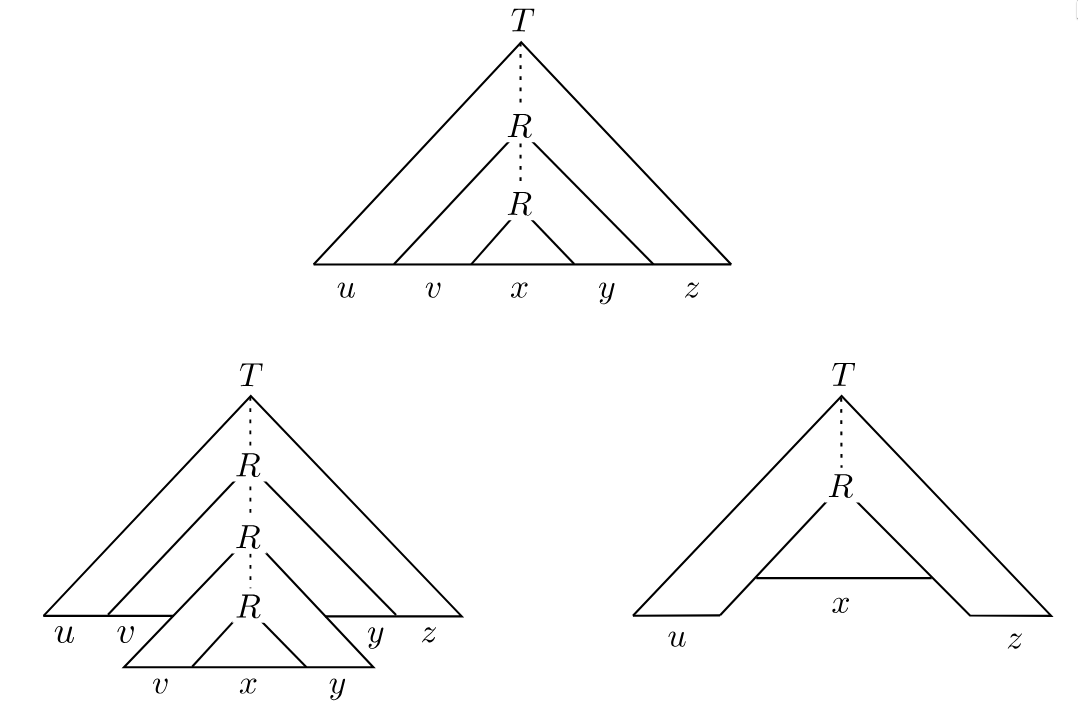
\includegraphics[scale=0.3]{img/2024-12-07-18-52-41.png}
\end{center}

}

Entriamo ora nei dettagli e proviamo a dimostrare in modo piu' formale tutte e tre le condizioni, oltre a vedere come calcolare la lunghezza di pompaggio $ p $:
\pf{Dimostrazione}{
  Sia $ G = (T, NT, R, S) $ una grammatica libera che genera $ L $. Sia $ b $ il massimo numero di simboli (sia $ T $ che $ NT $) che si trovano nella parte destra di una produzione in $ R $ ($ b = max \{|\alpha| \mid A \to \alpha \in R\} $). Possiamo assumere che $ b \geq 2 $, dato che altrimenti la grammatica sarebbe banale. In qualsiasi albero di derivazione generato da $ G $, il massimo numero di figli che puo' avere un nodo e' $ b $. In altre parole, ci saranno un massimo di $ b $ nodi che distano $ 1 $ dalla radice $ S $, al massimo $ b^2 $ che distano $ 2 $ e in generale un massimo di $ b^h $ nodi che distano esattamente $ h $ dalla radice. Quindi, se un albero e' alto $ h $ la stringa che genera e' lunga al massimo $ b^h $. Viceversa, se una stringa e' lunga almeno $ b^h + 1 $, allora il suo albero di derivazione sara' alto almeno $ h+1 $.
  \[
    |w| \geq b^h + 1 \implies \text{height(parseTree(w))} \geq h+1
  \]
  Sia $ |NT| $ il numero di nonterminali in $ G $, impostiamo la lunghezza di pompaggio nel seguente modo: $ p = b^{|NT|+1} $. Dato che $ b \geq 2 $, sappiamo che $ p > b^{|NT|} $, e quindi $ p \geq b^{|NT|}+1 $ (tecnicamente si puo' mettere maggiore stretto, ma per la dimostrazione non serve). Cosi' facendo, se $ s $ e' una stringa di $ L $ tale che $ |s| \geq p $, sappiamo che il suo albero di derivazione e' alto almeno $ |NT|+1 $:
  \[
    |w| \geq p = b^{|NT|+1} \geq b^{|NT|}+1 \implies \text{height(parseTree(w))} \geq |NT|+1
  \]
Notare che l'implicazione vale anche se poniamo $ b^{|NT|}+1 $ come pumping length, ma per garantire la terza condizione dobbiamo scegliere la lunghezza maggiore che puo' generare un albero alto $ |NT|+1 $, vedremo dopo perche'.

Per vedere come pompare una stringa $ w \in L, |w| \geq p $, chiamiamo $ \tau $ il suo albero di derivazione che ha il minor numero di nodi (questa condizione serve per garantire la seconda condizione). Sappiamo che $ \text{heigth}(\tau) \geq |NT|+1 $, ovvero che esiste un percorso dalla radice a una foglia lungo almeno $ |NT|+1 $. Contando la radice, ci sono $ |NT|+2 $ nodi lungo questo percorso, di cui uno e' la foglia che e' quindi un terminale. Quindi i restanti $ |NT| + 1 $ nodi sono tutti nonterminali, e per il \textit{pigeonhole principle} almeno uno si deve ripetere. Chiamiamo $ A $ il nonterminale che si ripete entro i $ |NT|+1 $ nonterminali "piu' in basso", ovvero piu' vicini alla foglia, lungo il percorso (questa scelta serve per garantire la terza condizione).

Dividiamo $ w $ in cinque parti $ uvxyz $ come nella figura. L' occorrenza superiore di $ A $ ha un sottoalbero piu' grande che genera $ vxy $, mentre quella piu' in basso ha un sottoalbero piu' piccolo e genera solo $ x $. Entrambe le sottostringhe sono generate dalla stessa variabile, quindi possiamo sostituire l'una con l'altra e ottenere un nuovo albero di derivazione valido. Sostituendo il minore con il maggiore ripetutamente ci da tutti gli alberi di derivazione per le stringhe $ uv^ixy^iz $ con $ i > 1 $. Sostituendo il maggiore con il minore otteniamo la stringa $ uxz $ (il caso in cui $ i = 0 $), quindi abbiamo stabilito che questa divisione soddisfa la prima condizione, vediamo le altre due:

Per la condizione 2, dobbiamo accertarci che $ u $ e $ y $ non siano entrambe $ \epsilon $. Usando l'eliminazione del not, assumiamo che siano entrambe $ \epsilon $ e dimostriamo il falso. Se fosse cosi', potremmo sostituire il sottalbero minore a quello maggiore ottenendo comunque la stringa iniziale ($ uxz = uv^ixy^iz $), pero' con un albero piu' piccolo. Ma questo e' assurdo, perche' come ipotesi avevamo stabilito che $ \tau $ fosse l'albero di derivazione di $ w $ con meno nodi. 

La terza condizione dice che $ |vxy| \leq p $. Questa e' la sottostringa generata dalla prima occorrenza di $ A $ (dalla radice verso le foglie), il cui sottoalbero e' alto al massimo $ |NT| + 1 $, dato che le due ripetizioni di $ A $ devono essere entro i $ |NT|+1 $ nonterminali piu' vicini alla foglia. La stringa piu' lunga che puo' generare un albero di quell'altezza e' $ b^{|NT|+1} = p $, quindi $ |vxy| \leq p $ come volevamo dimostrare.
}


\chapter{linguaggi liberi deterministici}

\section{PDA e linguaggi deterministici}
\subsection{PDA deterministici}
\dfn{PDA deterministico}{
    Un PDA $N=(\Sigma, Q, \Gamma, \delta, q_0, \bot, F)$ si dice \textbf{deterministico} sse:
    \begin{enumerate}
        \item \(\forall q \in Q, \; \forall z \in \Gamma, \; \big(\forall a \in \Sigma, \; (\delta(q, \epsilon, z) \neq \varnothing \implies \delta(q, a, z) = \varnothing)\big)\)
        \item $\forall q \in Q, \; \forall z \in \Gamma, \; \forall a \in (\Sigma \cup \{\epsilon\}), \; \big(|\delta(q, a, z)| \leq 1\big)$

    \end{enumerate}
}
Ovvero un PDA è libero deterministico sse in ogni configurazione, il PDA ha al massimo una transizione possibile per un dato stato, simbolo di input, e simbolo in cima alla pila e se ha una transizione $\epsilon$ disponibile allora non ha altri tipi di transizioni.

Quindi un PDA:
\begin{itemize}
    \item ha al massimo una transizione
    \item non ha conflitti tra transizioni $\epsilon$ e transizioni che leggono un simbolo
\end{itemize}
\subsection{Definizione di linguaggi liberi deterministici}
\dfn{Linguaggio libero deterministico}{
    Un linguaggio è \textbf{libero deterministico} se è accettato per stato finale da un DPDA
}
\teorema{
    la classe dei linguaggi liberi deterministici è includa propriamente nella classe dei linguaggi liberi :)
}
\esempio{
    \begin{itemize}
        \item Sia $L_1=\{ww^R\mid w\in\{a,b\}^*\}$ è libero, am si può dimostrare che non esiste un DPDA che lo riconosca, infatti con un DPDA non esiste un modo deterministico per riconoscere quando finisce $w$ e inizia $w^R$
        \item $L_2=\{wcw^R\mid w\in\{a,b\}^*\}$ è libero deterministico grazie al segnaposto $c$ è possibile riconoscere quando inizia $w^R$, si ha infatti:
        \begin{tikzpicture}[node distance=0cm]
            % States
            \node[state, initial] (q0) {\(q_0\)};
            \node[state, right of=q0] (q1) {\(q_1\)};
            \node[state, right of=q1] (q2) {\(q_2\)};
            \node[state, accepting, right of=q2] (q3) {\(q_3\)};
            
        
            % Transitions
            \draw (q0) edge[loop above] node[align=center] {\(a, Z \to aZ\) \\ \(b, Z \to bZ\)} (q0);
            \draw (q0) edge[below] node {\(c, Z \to Z\)} (q1);
            \draw (q1) edge[loop above] node[align=center] {\(a, a \to \varepsilon\) \\ \(b, b \to \varepsilon\)} (q1);
            \draw (q1) edge[below] node {\(\varepsilon, Z \to Z\)} (q2);
            \draw (q2) edge[below] node {\(\varepsilon, Z \to \varepsilon\)} (q3);
        
        \end{tikzpicture}        
    \end{itemize}
}

\teorema{
    Se $L$ è regolare, allora $\exists\; DPDA$ $N$ tale che $L=L[N]$ per stato finale
    
  %  \begin{center}
   %     \includegraphics[width=10cm]{gerarchia_automi.png}
    %\end{center}
    \begin{tikzpicture}
        % Cerchi per gli automi
        \draw[thick] (0, 0) circle (1.25cm) node[pos=0, yshift=0cm] {\textbf{DFA}};
        \draw[thick] (0, 0) circle (2.5cm) node[pos=0, yshift=1.75cm] {\textbf{DPDA}};
        \draw[thick] (0, 0) circle (3.75cm) node[pos=0, yshift=3.25cm] {\textbf{PDA}};
    
        % Cerchi per i linguaggi
        %\draw[thick] (8, 0) circle (1.5cm) node[pos=0, below right, xshift=-1.3cm] {\textbf{Linguaggi regolari}};
        %\draw[thick] (8, 0) circle (3cm) node[pos=0, above right, xshift=-2.1cm] {\textbf{Linguaggi liberi deterministici}};
        %\draw[thick] (8, 0) circle (4.5cm) node[pos=0, above right, xshift=-2.8cm] {\textbf{Linguaggi liberi}};
        
        % Annotazioni linguaggi
        \node[right] at (8, -1) {\(a^*b^*\)};
        \node[below] at (7, -2) {\(wcw^R\)};
        \node[below right] at (8.5, -3.5) {\(ww^R\)};
    \end{tikzpicture}
    
}
\pf{dimostrazione}{
    Se $L$ è regoalre, allora $\exists$ DFA $M$ tale che $L=L[M]$. A partire da $M$, posso costruire un DPDA $N$ si compore come $M$ senza mai manipolare lo stack, allora si che $L=L[N]$ per stato finale 
}
\subsubsection{Prefix propriety}
Si giunge così al seguente fatto:
\clm{}{}{
    Un linguaggio libero deterministico $L$ è riconosciuto da un $DPDA$ per pila vuota sse $L$ gode della "perfix propriety", ovvero 
    \[
        \nexists x,y\in L : x \text{ è prefisso di }y       
    \]
}
Pertanto si ha che:
\begin{itemize}
    \item Se $L$ è non gode della prefix propriety non può essere riconosciuto da un $PDPA$ per pila vuota
    \item Se $L$ è libero deterministico gode della prefix propriety, allora può essere riconosciuto da un $PDPA$ per pila vuota
    \item Se $L$ è libero deterministico, allora $L\$ =\{w\$ \mid w\in L\}$ gode della prefix propriety, infatti $L\$$ può essere riconosciuto da un $PDPA$ per pila vuota.
    
    Dove $\$\notin\Sigma$ ovvero $\$$ non è un simbolo dell'alfabeto di $L$, ma grazie ad esso alla fine di ogni linguaggio regolare vale la prefix propriety
\end{itemize}

\esempio{
    Sia $L_1 = \{a^nb^n\mid n\geq 0\}$ il seguente linguaggio che non gode della prefix propriety, in quanto $\epsilon\in L_1$ e $\epsilon$ è prefisso di $ab$

    \begin{tikzpicture}
        % States
        \node[state, initial, accepting] (q0) {\(q_0\)};
        \node[state, right of=q0] (q1) {\(q_1\)};
        \node[state, right of=q1] (q2) {\(q_2\)};
        \node[state, accepting, right of=q2] (q3) {\(q_3\)};
        
    
        % Transitions
        
        \draw (q0) edge[below] node {$\epsilon, Z/Z$} (q1);
        \draw (q1) edge[loop above] node[align=center] {$a,Z/AZ$} (q1);
        \draw (q1) edge[loop below] node[align=center] {$a,A/AA$} (q1);
        \draw (q1) edge[below] node {$b,A/\epsilon$} (q2);
        \draw (q2) edge[loop above] node[align=center] {$b,A/\epsilon$} (q2);
        \draw (q2) edge[below] node[align=center] {$\epsilon,Z/\epsilon$} (q3);
    
    \end{tikzpicture}
    
    Si ha quindi che il seguente linguaggio è riconosciuto da un DPDA \textit{per stato finale} e non \textit{per pila vuota}. Tuttavia il seguente linguaggio con il $\$\notin\Sigma$ è riconosciuto da un DPDA per \textit{per pila vuota}

    Sia $L_1\$$:


    \begin{tikzpicture}
        % States
        \node[state, initial] (q0) {\(q_0\)};
        \node[state, accepting, below of=q0] (q1) {\(q_1\)};
        \node[state, right of=q0] (q2) {\(q_2\)};
        \node[state, right of=q2] (q3) {\(q_3\)};
        
    
        % Transitions
        
        \draw (q0) edge[below] node {$a, Z/AZ$} (q2);
        \draw (q0) edge[left] node {$\$,Z/\epsilon$} (q1);
        \draw (q3) edge[loop above] node[align=center] {$b,A/\epsilon$} (q3);
        \draw (q3) edge[left] node[align=right] {$\$, Z/\epsilon$} (q1);
        \draw (q2) edge[loop above] node[align=center] {$a,A/AA$} (q2);
        \draw (q2) edge[below] node[align=center] {$b,A/\epsilon$} (q3);
    
    \end{tikzpicture}

    Si verifichi, infatti, come egli venga riconosciuto per pila vuota

}

\esempio{
    Sia $L_3 = \{a^nb^m\mid n\geq m \geq 0\}$ e dato che $\epsilon\in L_3$ tale linguaggio non gode della prefix propriety

    \begin{tikzpicture}
        \node[state, initial, accepting] (q0) {$q_0$};
        \node[state,  accepting, right of=q0] (q1) {$q_1$};
        \node[state,  accepting, right of=q1] (q2) {$q_2$};
        \node[state,  accepting, right of=q2] (q3) {$q_3$};

        \draw (q0) edge[above] node[align=center] {$a,Z/AZ$} (q1);
        \draw (q1) edge[above] node[align=center] {$b,A/\epsilon$} (q2);
        \draw (q2) edge[above] node[align=center] {$\epsilon, Z/\epsilon$} (q3);
        \draw (q2) edge[loop above] node[align=center] {$b,A/\epsilon$} (q2);
        \draw (q1) edge[loop above] node[align=center] {$b,A/AA$} (q1);
        
    \end{tikzpicture}

    e sia $L_3\$$:

    \begin{tikzpicture}
        \node[state, initial] (q0) {$q_0$};
        \node[state,  right of=q0] (q1) {$q_1$};
        \node[state,  right of=q1] (q2) {$q_2$};
        \node[state,  above of=q1] (q3) {$q_3$};
        \node[state,  below of=q1] (q4) {$q_4$};

        \draw (q0) edge[above] node[align=center] {$a,Z/AZ$} (q1);
        \draw (q0) edge[left] node[align=center] {$\$,Z/\epsilon$} (q3);
        \draw (q1) edge[above] node[align=center] {$b,A/\epsilon$} (q2);
        \draw (q1) edge[left] node[align=center] {$\$,A/\epsilon$} (q4);
        \draw (q2) edge[right] node[align=center] {$\$, Z/\epsilon$} (q3);
        \draw (q2) edge[right] node[align=center] {$\$, A/\epsilon$} (q4);

        \draw (q2) edge[loop right] node[align=center] {$b,A/\epsilon$} (q2);
        \draw (q1) edge[loop above] node[align=center] {$b,A/AA$} (q1);
        \draw (q4) edge[loop left] node[align=center] {$\epsilon,X/\epsilon$} (q4);

        
    \end{tikzpicture}


}

\subsubsection{non ambiguità dei linguaggi liberi deterministici}
\mprop{}{
    Se $L$ è libero deterministico, ovvero riconosciuto da un $DPDA$ per \textit{stato finale}, allora $L$ è generabile da una \textbf{grammatica libera non ambigua}.
    
    Si ha quindi che i \red{linguaggi liberi deterministici non sono ambigui}
}


%! errori e non capisco il motivo puercos zios
\subsubsection{Proprietà dei linguaggi liberi deterministici}

I lunguaggi liberi deterministici presentano le seguenti proprietà:
\mprop{chiusura solo per complementazione}{
    Sia $L$ un linguaggio libero deterministico, allora questo è chiuso per complementazione, ovvero:
\[
        (\exists \; \text{DPDA} \; N \; : \; L = L(N)) \implies (\exists \; \text{DPDA} \; N' \; : \; \overline{L} = L(N')) \quad \text{dove} \quad \overline{L} = \Sigma^* \setminus L
\]
}
\dimostrazione{
    Bisogna rendere totale la $\delta$ di $N$, eventualmente aggiungendo stati non finali, e poi $N'$ si ottiene da questo $N$ "aumentato", semplicemente scambiando \red{finali e non finali} 
}

\mprop{
    Non chiusura per intersezione
}{
    Un linguaggio libero deterministico non è chiuso per intersezione
}
\esempio{
    $L_1 =\{a^nb^nc^m\mid n,m\geq 0\}$ è libero deterministico\\
    $L_2 =\{a^mb^nc^n\mid n,m\geq 0\}$ è libero deterministico\\
    ma\\
    $L_1\cap L_2 =\{a^nb^nc^n\mid n\geq 0\}$ non è libero!

}

\mprop{
    non chiusura per unione
}{
    Un linguaggio libero deterministico non è chiuso per unione
}
\dimostrazione{
    Assumiamo per assurdo che un linguaggio libero deterministico sia chiuso per unione, allora:
    \[
        L_1\cap L_2 = \overline{\overline{L_1}\cup \overline{L_2}}    
    \]

    Per questo fatto e la proprosizione precedente si è verificato un assurdo
}

\subsection{Analizzatori sintattici: parser}
\begin{tikzpicture}[node distance=2cm]

        % Nodes
        \node (grammar) [startstop] {Grammatica Libera};
        \node (algorithm) [process, right of=grammar, xshift=4cm] {Algoritmo di \\ Costruzione (YACC)};
        \node (parser) [startstop, right of=algorithm, xshift=4cm] {Parser};
        \node (tokens) [startstop, below of=grammar, yshift=-2.5cm] {Lista di Token};
        \node (parser2) [process, right of=tokens, xshift=4cm] {Parser};
        \node (tree) [startstop, right of=parser2, xshift=4cm] {Albero di Derivazione};
        \node (additional) [below of=parser] {fondamentalmente un \\$DPDA$ con output};
        
        % Arrows
        \draw [arrow] (grammar) -- (algorithm);
        \draw [arrow] (algorithm) -- (parser);
        \draw [arrow] (tokens) -- (parser2);
        \draw [arrow] (parser2) -- (tree);
        \draw [wavearrow] (additional) -- (parser);
        
        % Additional text
        
        
        
        
\end{tikzpicture}

I parser possono essere:
\begin{itemize}
    \item \textbf{nondeterministici}: se, durante la ricerca di una derivazione, si scopre che una scelta è improduttiva e non porta a riconoscere l'input, \red{il parser torna indietro} (\textit{backtracking}), disfa parte della derivazione appena costruita e scegli un'altra produzione, \red{tornando a leggere parte dell'input}
    \item \textbf{deterministici}: leggono l'input una sola volta ed \red{ogni loro decisione è definitiva}
\end{itemize}

entrambi cercano di sfruttare informazioni dall'input per guidare la ricerca della derivazione

\subsubsection{introduzione al top-down parsing}
\dfn{}{
    Data $G=(NT,T,S,R)$ lebera, costruiamo il $PDA\;M=(T,\{q\}, T\cup NT, \delta, q, S, \varnothing)$, che riconosce per pila vuota, dove $\delta:Q\times(\Sigma\cup\{\epsilon\})\times\Gamma→Q\times\Gamma^*$ è definita:
    \begin{itemize}
        \item \textbf{espandi}: $(q,\beta)\in \delta(q,\epsilon, A)$ se $A\to\beta\in R$ 
        \item \textbf{consuma}: $\forall a\in T((q,\epsilon)\in \delta(q,a, a))$ 
    \end{itemize} 
    Tale che $L(G)=P[M]$ (riconoscimento per pila vuota)
}

Quindi, grazie alla prima regola se il simbolo in cima alla pila è un non terminale $A$, l'automa può espanderlo sostituendolo con la produzione $\beta$, come descritto nelle regole $R$ della grammatica, mentre secondo la regola di consumazione si ha che se il simbolo sulla cima della pila e il simbolo corrente della stringa in input sono entrambi a, allora l'automa può eliminare quel simbolo dalla pila e procedere nella lettura dell'input.

\esempio{
    Sia $G$ la seguente grammatica:
    \[
        \begin{array}{l}
            S\to aSb\mid \epsilon
        \end{array}    
    \]

    Si ha che $S\implies aSb \implies aaSbb \implies aabb$

    \begin{center}
       \begin{tikzpicture}
        \node[state] (q) {$q_0$};
        \draw (q) edge[loop right] node[align=center] {$b,b/\epsilon$} (q);
        \draw (q) edge[loop above] node[align=center] {$a,a/\epsilon$} (q);
        \draw (q) edge[loop left] node[align=center] {$\epsilon,S/\epsilon$} (q);
        \draw (q) edge[loop below] node[align=center] {$\epsilon,S/aSb$} (q);
    \end{tikzpicture} 
    \end{center}

    Si osservi che il seguente automa che riconosce il linguaggio della grammatica $S$ non è un PDPA

    Nella maggior parte delle configurazioni standard di un Pushdown Automaton (PDA) utilizzato per il parsing top-down, la pila viene inizializzata con il simbolo iniziale della grammatica, nel nostro caso, quindi, la serie di passaggi che porteranno a riconoscere il linguaggio sarà:
    \[
        \begin{array}{l}
            (q,aabb,S) \vdash (q,aabb,aSb)\\
            \vdash (q,abb,Sb)\vdash (q,abb,aSbb)\\
            \vdash  (q,bb,Sbb)\vdash (q,bb,bb)\\
            \vdash (q,b,b)\vdash (q,\epsilon,\epsilon)
        \end{array}
    \]
    che costruisce il seguente albero di derivazione 
    \begin{center}
        \begin{tikzpicture}
            \Tree [.S 
                        a
                        [.S
                            a
                            [.S
                                $\epsilon$
                            ]
                            b
                        ]
                        b
                ]
        \end{tikzpicture}
    \end{center} 

    Si ha, quindi:
    \begin{itemize}
        \item derivazione canonica a sx (leftmost)
        \item costruzione dell'albero dall'alto in basso
    \end{itemize}

    %TODO triangolo
}

Tuttavia in questo esempio è facile verificare che il parser è nondeterministico, infatti l'automa è un $PDA$, tuttavia questo nondeterminismo può essere risolto \red{scegliendo la produzione in baso al simbolo di lettura nell'input} (\textbf{look-ahead}), ad esempio:
\begin{itemize}
    \item se leggo $a$, espando $S\to aSb$
    \item se leggo $b$, espando $S\to \epsilon$
\end{itemize}

\begin{center}
  \begin{tabular}{rrr}
    \textbf{input} & \textbf{stack}&\textbf{azione}\\
    $\underline{a}abb\$$&$S$&leggo $a$ e espando in $aSb$ \\
    & $\underline{a}Sb$&consumo\\
    $\underline{a}bb\$$&$Sb$&leggo $a$ e espando in $aSb$\\
    &$\underline{a}Sbb$&conumo\\
    $\underline{b}b\$$ & $Sbb$&leggo $b$ e espando in $\epsilon$\\
    &$\underline{b}b$&consumo\\
    $b\$$&$b$&leggo $b$ e espando in $\epsilon$ \\
    $\$$ & $\epsilon$& fin
\end{tabular}  
\end{center}

\nt{
    Non tutte le grammatiche sono adatte per il top down-parser
}
\esempio{
    Sia $G$ la segnuete grammatica:
    \[
        S\to Sb\mid a        
    \]
    e $L(G)=ab^*$ (linguaggio regolare semplice)

    L'automa che riconosce il linguaggio è:
    \begin{center}
        \begin{tikzpicture}
         \node[state] (q) {$q$};
         \draw (q) edge[loop right] node[align=center] {$b,b/\epsilon$} (q);
         \draw (q) edge[loop above] node[align=center] {$a,a/\epsilon$} (q);
         \draw (q) edge[loop left] node[align=center] {$\epsilon,S/a$} (q);
         \draw (q) edge[loop below] node[align=center] {$\epsilon,S/Sb$} (q);
     \end{tikzpicture} 
     \end{center}

     Con i seguenti passaggi:
     \[
        (q,ab,S)\vdash(q,ab,Sb)\vdash(q,ab,Sbb)\vdash\dots   
     \]
     Qui il determinismo non funziona, infatti se vogliamo espandere quando leggiamo $a$ in input non possiamo anche consumare, pertnato l'automa espanderà all'infinito

     Occorre manipolare la grammatica affinche non vi siano ricorsioni sinistre
}

\subsubsection{
    Introduzione al botto-up parsing
}
\clm{}{}{
    Data una grammatica libera $G = (NT, T, R, S)$, costruiamo un $PDPA\;M = (T,\{q\},T\cup NT\cup\{Z\},\delta,q,Z,\varnothing)$ che riconosce $L(G).\$$ dove:
    \begin{itemize}
        \item \textbf{shift}: $\forall a \in T,\Big(\forall X\in T\cup NT\cup Z,\big((q,aX)\in \delta(q,a,Z)\big)\Big)$
        \item \textbf{reduce}: $(A\to\alpha R)\implies(q,A)\in\delta (q,\epsilon,\alpha^R)$ 
        
        Con $\alpha^R$ una generalizzazione dei $PDA$ in cui si consuma una stringa sulla pila anziché solo il top
        \item \textbf{accept}: \((q,\epsilon)\in \delta (q,\$,SZ)\)
        
        Con $S$ che deve essere alla fine sulla pila e $\$$ simbolo di fine input
    \end{itemize}
}

Cominciamo subito con un esempio
\esempio{
    Sia $G$ la seguente grammatica:
    \[S\to aSb\mid ab\]

    
\begin{center}
    \begin{tikzpicture}
        \node[state] (q) {$q$};
        
        \draw (q) edge[loop above] node[align=center] {$a,a/\epsilon$} (q);
        \draw (q) edge[loop right] node[align=center] {$b,b/\epsilon$} (q);
        \draw (q) edge[out=330, in=300, looseness=8] node[align=center] {$c,c/\epsilon$} (q);
        \draw (q) edge[out=210, in=240, looseness=8] node[align=center] {$d,d/\epsilon$} (q);
        \draw (q) edge[loop left] node[align=center] {$e,e/\epsilon$} (q);
    \end{tikzpicture}
\end{center}

\begin{center}
    \begin{tabular}{lll}
        \textbf{stack}&\textbf{input}&\textbf{azione}\\
        $Z$ & $aabb\$$ & shift\\
        $Za$ & $abb\$$ & shift\\
        $Zaa$ & $bb\$$ & shift\\
        $Zaab$ & $b\$$ & reduce $S\to ab$\\
        $ZaS$&$b\$$ & shift \\
        $ZaSb$ & $\$$ & reduce $S\to aSb$\\
        $ZS$ & $\$$ & \textit{accept}\\
        $\epsilon$ & $\epsilon$ &
    \end{tabular}
\end{center}

In passaggi, $S\implies aSb \implies aabb$. Viene prodotto il seguente albero di derivazione:

\begin{center}
    \begin{tikzpicture}
    \Tree[.S 
        a
        [.S
            a
            b
        ]
        b
    ]
    \end{tikzpicture}    
\end{center}

Si può verificare come come la costruzione dell'input sia:
\begin{itemize}
    \item \textbf{left-to-right} (come leggo l'input)
    \item \textbf{right-derivatione}
    \item 
\end{itemize}

Tuttavia  è facile verificare che c'è molto nondeterminismo:
\begin{itemize}
    \item Conflitti: Shift-Reduce
    \begin{enumerate}
        \item $zaab \quad b\$ \quad$ (può fare shift)
        \item $zaabb \quad \$ \quad$ (ma è un percorso infruttuoso)
    \end{enumerate}
    \item Conflitti: Reduce-Reduce
    
    Più riduzioni possibili (non ci sono in quest'esempio, ma con grammatiche più complesse è possibile)

\end{itemize}
}

Per ottenere un DPDA, serve introdurre informazioni aggiuntive per risolvere i conflitti:
\begin{itemize}
    \item \textbf{Più stati:} (o strutture particolari di supporto alle decisioni, come un DFA dei prefissi validi).
    \item \textbf{Look-ahead:} (guardare l'input in avanti).
\end{itemize}

Vediamo un esempio più corposo relativo alle grammatiche delle espressioni aritmetiche:

\esempio{
    Sia $G$ tale grammatica:
    \[
        \begin{aligned}
            & E \to T + E \mid T \\
            & T \to T \times A \mid A \\
            & A \to a \mid b \mid (E)
        \end{aligned}
    \]
    Si ha:

    %! modificare il reduce
    \[
        \begin{array}{|c|l|}
        \hline
        \textbf{G} & \textbf{M} \\
        \hline
        & t_0 : \delta(q, a, X) = (q, aX) \; \forall aX \quad \text{SHIFT} \\
        \text{(R1)} \; E \to T + E  & t_1 : \delta(q, \epsilon, E + T) = (q, E) \\
         \text{(R2)} \; E \to T & t_2 : \delta(q, \epsilon, T) = (q, E) \\
        \text{(R3)} \; T \to T \ast A & t_3 : \delta(q, \epsilon, A \ast T) = (q, T) \quad \text{REDUCE} \\
        \text{(R4)} \; T \to A & t_4 : \delta(q, \epsilon, A) = (q, T) \\
        \text{(R5)} \; A \to (E) & t_5 : \delta(q, \epsilon, (E)) = (q, A) \\
        \text{(R6)} \; A \to a & t_6 : \delta(q, \epsilon, a) = (q, A) \\
        \text{(R7)} \; A \to b & t_7 : \delta(q, \epsilon, b) = (q, A) \\
                            & t_8 : \delta(q, \$, EZ) = (q, \epsilon) \quad \text{ACCEPT} \\
        \hline
        \end{array}
    \]
    La cui sequenza è:
    \[
        a*(b)\Leftarrow A*(b) \Leftarrow T*(b)\Leftarrow T*(A) \Leftarrow T*(T)\Leftarrow T*(E)\Leftarrow T*A \Leftarrow T \Leftarrow E
    \]

    La cui pila-stack-input è:
    \[
        \begin{array}{|c|c|c|}
            \hline
            \textbf{Stack} & \textbf{Input} & \textbf{Action} \\
            \hline
            Z & a \ast (b) \$ & \text{shift} \\
            Z a & \ast (b) \$ & \text{reduce } R_6 \\
            Z A & \ast (b) \$ & \text{reduce } R_4 \\
            Z T & \ast (b) \$ & \text{shift} \\
            Z T \ast & (b) \$ & \text{shift} \\
            Z T \ast ( & b) \$ & \text{shift} \\
            Z T \ast ( b & ) \$ & \text{shift} \\
            Z T \ast ( b ) & \$ & \text{reduce } R_7 \\
            Z T \ast ( A & ) \$ & \text{reduce } R_4 \\
            Z T \ast ( T & ) \$ & \text{reduce } R_2 \\
            Z T \ast ( E & ) \$ & \text{shift} \\
            Z T \ast ( E ) & \$ & \text{reduce } R_5 \\
            Z T \ast A & \$ & \text{reduce } R_3 \\
            Z T & \$ & \text{reduce } R_2 \\
            Z E & \$ & \text{accept} \\
            \epsilon &\epsilon & \\
            \hline
        \end{array}
    \]

    Il cui albero di derivazione:
    \begin{center}
        \begin{tikzpicture}
        \Tree[.E 
            [.T
                [.T
                    [
                        .A
                        [
                            .a
                        ]
                    ]
                ]
                *
                [
                    .A
                    $($
                    [
                        .E
                        [
                            .T
                            [
                                .A
                                [
                                    .b
                                ]
                            ]
                        ]
                    ]
                    $)$
                ]
            ]
        ]
        \end{tikzpicture}    
    \end{center}



}

L'automa è non deterministico perché:
\begin{enumerate}
    \item Chi ha precedenza tra \textit{shift} e \textit{reduce}?
    
    \textbf{Ad esempio:}
    \begin{enumerate}
        \item[1)] $Z a \quad * \, (b) \, \$ \quad$ \textit{shift}
        \item[2)] $Z a * \quad (b) \, \$ \quad$ non buono! Qui \textit{reduce} è in conflitto con \textit{shift}!
    \end{enumerate}
    
    \textbf{Altro esempio:}
    \begin{enumerate}
        \item $Z T \quad * \, (b) \, \$ \quad$ \textit{reduce } $R_2$
        \item $Z E \quad * \, (b) \, \$ \quad$ non buono! Qui \textit{shift} è in conflitto con \textit{reduce}!
    \end{enumerate}
    
    \item Chi ha precedenza tra due diverse \textit{reduce}?
    
    \textbf{Ad esempio:}
    \begin{enumerate}
        \item $Z T * A \quad \$ \quad$ \textit{reduce } $R_3$
        \item $Z T \quad \$$
        \item $Z T * T \quad \$ \quad$ se faccio, \textit{reduce } $R_4$ \\
        Qui \textit{reduce} $R_3$ è in conflitto con \textit{reduce} $R_4$!
    \end{enumerate}
    
    È buona norma scegliere in modo tale che ciò che si trova nella pila sia un prefisso (a rovescio) di una parte destra di una produzione della grammatica.
    
    \textbf{Ad esempio:}
    \begin{enumerate}
        \item $Z a$
        \item $Z A$ con la ``norma'' produco chi coincide con ciò che è un prefisso di una parte destra che comincia con $A$.
    \end{enumerate}
\end{enumerate}

\subsubsection{problema con le pruzioni $\epsilon$}
Sia la produzione $S\to \epsilon$

TODO! NON HO CAPITO


\section{Semplificazione delle grammatiche}
Per avere \textbf{PDA} efficienti e con minor non determinismo è necessario semplificare le grammatiche. Ad esempio:
\begin{itemize}
    \item Eliminare le produzioni $\epsilon$ (del tipo $A\to\epsilon$) inadatte al bottom up parsing
    \item Eliminare le \red{produzione unitarie} (del tipo $A\to B$ che possono creare dei cicli $A \implies^+ A$) 
    \item Eliminare \red{simboli inutili}, cioè quei terminali e non terminali che non sono raggiungibili/generabili a partire dal simbolo inziale $S$
    
    es. gli stati d'errore 

    \item  Eleminare \red{la ricorsione sinistra} (del tipo $A \to A\alpha$), perché inadatte al top - down parsing
    \item \red{fattorizzare} le grammatiche, per ottenere grammatiche con meno non determinismo nel top-down parsing
\end{itemize}

\subsection{Eliminare le produzioni $\epsilon$}
Per fare ciò si usi un algoritmo che ha:
\begin{itemize}
    \item in \red{input}: una $G$ libera con produzione $\epsilon$ 
    \item in \red{output}: una $G'$ libera senza produzione $\epsilon$ tale che $L(G') = L(G)\backslash\{\epsilon\}$ 
\end{itemize}

\osservazione{
    Se $\epsilon \in L(G)$ e si vuole ottenere una $G''$ t.c. $L(G)= L(G'')$, basta considerare $G' = (NT,T,S,R')$ e definire $G'' = G' \cup \{S' \to \epsilon | S\}$ t.c.
    \[
        G'' = (NT\cup\{S'\},T,S',R'\cup \{S' \to \epsilon|S\})
    \]
}
\subsubsection{simboli annullabili}
Per l'algoritmo occorre innanzi tutto definire i \textbf{simboli annullabili}
\dfn{simboli annullabili}{ \label{semplificazioneGram}
    I \textbf{simboli annullabili} sono quei non terminali tale che possono riscriversi in uno o più passi in $\epsilon$, ovvero:
    \[
        N(G) = \{A\in NT | A \implies^{+} \epsilon\}    
    \]
    Dove $N(G)$ è l'insieme dei simboli annullabili e viene calcolato induttivamente come segue:
    \begin{itemize}
        \item $N_0 (G) = \{A\in NT | A\to \epsilon \}$, questo è il caso in cui un non terminale $A$ viene riscritto direttamente in $\epsilon$ tramite una produzione
        \item $N_{i+1}(G) = N_i (G) \cup\{B\in NT | B \to c_1,\dots, c_k \in \mathbb{R}\text{ e } c_1,\dots, c_k \in N_i(G)\}$ questo è il caso in cui un non terminale $B$ possa essere ricondotto a a $\epsilon$ in più passi
    \end{itemize}
}

Ovviamente $\exists i_c$ tale che $N_{i_c}(G)=N_{i_c+1}(G)$, cioè che ad un certo punto non aggiungo nessun altro $B$ all'insieme ($NT$ è finito)
\teorema{
    L'insieme $N(G) = N_{i_c}(G)$ è esattamente l'insieme di tutti i simboli annullabili
}

\subsubsection{algoritmo per il calcolo della grammatica}


Una volta calcolato \( N(G) \) per \( G = (N, T, S, R) \), costruiamo la grammatica \( G' = (N, T, S, R') \) dove per ogni produzione \( A \rightarrow \alpha \in R \) con \( \epsilon \not\in \alpha \), in cui occorrono simboli annullabili \( Z_1, \ldots, Z_k \), mettiamo in \( R' \) tutte le produzioni del tipo \( A \rightarrow \alpha' \) dove \( \alpha' \) si ottiene da \( \alpha \) cancellando tutti i possibili sottoinsiemi di \( Z_1, \ldots, Z_k \) (incluso \( \varnothing \)), ad eccezione del caso in cui \( \alpha' \) risulta \( \epsilon \), in altre parole si creano tutte le possibili combinazioni di $\alpha$ eliminando uno o più di questi simboli $Z_1,\dots,Z_n$:

\begin{itemize}
    \item in \( G' \) non mettiamo produzioni \( A \rightarrow \epsilon \in R \),
    \item in \( G' \) non introduciamo mai produzioni del tipo \( A \rightarrow \epsilon \).
\end{itemize}

\teorema{
    Data una grammatica libera \( G \), la grammatica \( G' \) determinata dall'algoritmo sopra non ha \( \epsilon \)-produzioni, e \( L(G') = L(G) \setminus \{\epsilon\} \)
}

\esempio{
    Sia $G$ una grammatica tale che:
    \[
        G = \begin{cases}
            S \to AB \\
            A\to aAA\mid\epsilon\\
            B\to bBB\mid\epsilon
        \end{cases}    
        \quad
        N_0(G)=\{A,B\} \text{ e }N_1(G)=\{A,B,S\} = N(G)
    \]
    Quindi tutti sono simboli annullabili

    Adesso procedo con l'algoritmo, procedo per ogni simbolo annullabili
    \begin{itemize}
        \item $S\to AB$: secondo l'algoritmo devo cancellare in tutti i modi possibili i simboli non terminali che compaiono nella parte destra della produzione. In questo caso dobbiamo considerare 4 casi:
        \begin{itemize}
            \item $\emptyset\implies S\to AB$, rinuncio a cancellare
            \item $\{B\}\implies S\to A$, se cancello $B$ rimane $A $nella parte destra
            \item $\{A\}\implies S\to B$
            \item $\{A,B\}\implies S\to \epsilon$ dato che non devo mai introdurre produzioni del tipo \( A \rightarrow \epsilon \) \red{non posso cancellare $A$ e $B$}
        \end{itemize}
        Unisco i vari sottoinsiemi e si ha:
        \[
            S\to AB|B|A
        \]
        \item $A\to aAA\in R$. dobbiamo considerare 4 casi:
        \begin{itemize}
            \item $\emptyset\implies A\to aAA$
            \item $\{A\}\implies A\to aA$
            \item $\{A,A\}\implies A\to a$
        \end{itemize}
        Quindi si ha:
        \[
            A\to aAA|aA|a    
        \]
        \item si ha la stessa cosa con $B$, quindi cancellarehe verrà trasformato in 
        \[
            B\to bBB|bB|b    
        \]
        Così la nuova grammatica sarà:
        \[
            G' = \begin{cases}
                S\to AB|A|B\\
                A\to aAA|aA|a\\
                B\to bBB|bB|b
            \end{cases}    
        \]
    \end{itemize}
}
\subsection{Eliminazione delle produzioni unitarie}


\dfn{Produzione unitaria}{
    Una produzione si dice \textbf{unitaria} quando $A\to B$ si ha che $A,B\in NT$
}

\subsubsection{coppie unitarie}
Per eliminare queste produzioni unitarie si deve però calcolare quelle che sono definite le "coppie unitarie"
\dfn{Coppia unitaria}{
    Una coppia $(A,B)$ si dice \textbf{unitaria} qunado $A\implies^* B$ (quindi quando $A$ può riscriversi in 0 o più passi nel non terminale $B$) usando solo produzioni unitarie. 
    
    Vi è qui ripostata la definizione induttiva:
    \begin{itemize}
        \item $U_0(G) = \{(A,A)|A\in NT\}$, quindi ogni non terminale fa coppia con se stesso
        \item $U_{i+1}(G) = U_i (G)\cup \{(A,C)|(A,B)\in U_i(G)\}$ e $B\to C\in R$, quindi è l'insieme delle coppie al passo $i$ unito alle coppie alle coppie $(A,C)$ tali che $(A,B)$ sono coppie presenti nell'insieme dell'iterazione precedente e $B\to C \in R$
    \end{itemize} 
}

Anche in questo caso $\exists i_c$ t.c. $U_{i_c}(G) = U_{i_c+1}(G)$ dato che $NT$ è finito. Pertanto per definizione si ha che $U(G) = U_{i_c}(G)$, detto insieme di tutte le coppie unitarie

\subsubsection{algoritmo per il calcolo dell'eliminazione delle produzioni unitarie}

Data $G = (N, T, R, S)$ libera, si definisce una $G' = (N, T, R', S)$ dove, per ogni $(A, B) \in U(G)$, $R'$ contiene 
tutte le produzioni $A \rightarrow \alpha$, dove $B \rightarrow \alpha \in R$ 
e non è unitaria

\osservazione{
    Poiché, per ogni $A \in N$, la coppia $(A, A) \in U(G)$, $R'$ contiene tutte le produzioni non unitarie di $R$ e in aggiunta un po' di altre.
}

\teorema{
    Sia $G = (NT, T , R, S)$ libera e sia $U(G)$ l'insieme selle sue coppie unitarie. Sia $G' = (NT, T, R', S)$ la grammatica ottenuro dall'algoritmo $G'$ non ha produzione unitarie e $L(G) =  L (G')$
}

Esempietto:
\esempio{
    Prediamo con esempio la grammatica non ambigua $E$ delle espressioni aritmetiche:
    \[
        E = \begin{cases}
            E\to E+ T|T\\
            T\to T * A|A\\
            A\to a|b|(E)
        \end{cases}       
    \]
    Si noti subito che ha 2 produzioni unitarie: $E\to T \text{ e }T\to A$.
    Iniziamo a calcolare l'insieme delle coppie unitarie:
    \begin{itemize}
        \item $U_0(G) = \{(E,E),(T,T),(A,A)\}$ e grazie al cuzzo
        \item $U_1(G) =U_0(G) \cup \{(E,T),(T,A)\}$
        \item $U_2(G) =U_1(G) \cup \{(E,A)\} = U_3(G) = U(G)$ dato che da che da $E$ si arriva ad $T$ e si arriva $A$
    \end{itemize}

    Per calcolare la grammatica $G'$ devo prendere tutte le produzioni non unitarie della grammatica originale, ovvero: 
    \[
        G' = \begin{cases}
            E\to E+T\\
            T\to T\times A\\
            A\to a|b|(E)
        \end{cases}
    \]
    In aggiunta:
    \[
        \begin{cases}
            E\to E+T  & \text{ perché } (E,T)\in U_1(G)\\
            T\to a|b|(E) & \text{ perché } (T,A)\in U_1(G)\\
            E\to a|b|(E) & \text{ perché } (E,A)\in U_2(G)
        \end{cases}
    \]
    Pertanto $G'$ sarà:
    \[
        G' = \begin{cases}
            E\to E+T | T\times A|a|b|(E)\\
            T\to T\times A|a|b|(E) \\
            A\to a | b | (E)
        \end{cases}    
    \]

    Sia ha che non contiene produzioni unitarie ed è equivalente a $G$
}
\subsection{Rimuovere i simboli inutili}

\dfn{Simboli generatori, raggiungibili e utili}{
    Un simbolo $X\in T\cup NT$ è 
    \begin{itemize}
        \item Un \red{generatore} $\iff \exists w \in T^*$ con $x\implies^* w$ 
        
        Quindi un generatore è o un terminale (un simbolo può riscriversi in se stesso) oppure un non terminale che in uno o più passi. è definito induttivamente come segue:
        \begin{itemize}
            \item $G_0(G)= T$ se $a\in T, a\implies^* a$ (quindi tutti i terminali sono generatori)
            \item $G_{i+1}(G)= G_i(G)\cup \{B\in NT|B \to C_1,\dots C_k \in R \land C_1,\dots, C_k \in G_i(G)\}$
        \end{itemize}
        \item Un \red{raggiungibile} $\iff (\exists\alpha,\beta \in (T\cup NT)^*.( S\implies^*\alpha X \beta))$. Sono definiti induttivamente:
        \begin{itemize}
            \item $R_0(G) = \{S\}$
            \item $R_{i+1}(G) = R_i(G)\cup\{x_1, \dots, x_k\} \forall B\in R_i (G), B\to x_i,\dots, x_k \in R$ 
        \end{itemize}
        \item \red{utile} sse è sia un generatore e sia raggiungibile, ovvero se $S\implies^* \alpha X \beta\implies^* x\in L(G)$ cioè $X$ compare in almeno una derivazione di una stringa $z\in L(G)$
    \end{itemize}
}


\subsubsection{algoritmo per l'eliminazione dei simboli inutili}
\begin{enumerate}
    \item Prima di tutto elimino tutti i non-generatori (e tutte le produzione che usano almeno uno di questi)
    \item Poi dalla nuova grammatica, elimino tutti i non - raggiungibili (E tutte le produzioni che li usano)
\end{enumerate}

\teorema{
    Sia $G=(NT,T,R,S)$ una grammatica libera t.c. $L(G) \neq \emptyset$
    \begin{itemize}
        \item Sia $G_1$ la grammatica che si ottiene da $G$ eliminando tutti i simboli che non a appartengono a $G(G)$ (insieme dei generatori), e tutte le produzioni che fanno uso di algoritmo di tali simboli
        \item Sia $G_2$ la grammatica che si ottiene da $G_1$ eliminando tutti i simboli che non appartengono a $R(G)$, e tutte le produzioni che fanno uso di almeno uno di tali simboli 
    \end{itemize}
    
    Allora $G_2$ non ha simboli inutili e $L(G_2) = L(G)$
}
\dimostrazione{
     La dimostrazione si divide nelle due parti dell'enunciato:
     \begin{itemize}
        \item $L(G_2 )\subseteq L (G)$ è ovvio, dato che $G_2$ contiene meno produzioni di $G$
        \item $L(G)\subseteq L(G_2)$: dobbiamo dimostrare che $S\implies^*_G w$ (ovvero se $S$ deriva $W$ usando le produzioni di $w$) allora $S\implies^*_{G_2 }w$
        
        Si ha che ogni simbolo usato in $S\implies^*_G w$ è, ovviamente, sia raggiungibile sia generatore

        Quindi quelle derivazioni è anche una derivazione per $G_2$

        Q.e.d.
     \end{itemize}
}

\osservazione{
    L'ordine dei due generatori è importante! 
    \begin{itemize}
        \item prima elimino i non-generatori
        \item poi i non - raggiungibili
    \end{itemize}
    ma se inverto l'ordine, allora può capitare che non elimino tutti i simboli inutili
}


Esempietto di eliminazione di tutti quei simboli non utili (inutili)

\esempio{
    Si parta da questa grammatica:
    \[
        G = \begin{cases}
            S \to AB|a \\
            B\to b
        \end{cases}       
    \]
    Poiché $a\implies^*a, b\implies^*b, S\implies^*a, B\implies^*b$ si ha che i generatori saranno $\{S,B,a,b\}$ (dove manca $A$). Possiamo così eleminare tutte le produzioni che includono $A$:
    \[
        G' = \begin{cases}
            S\to a\\
            B\to b
        \end{cases}    
    \]
    Adesso posso eliminare tutti i non raggiungibili da $S$, che in questo caso l'unico è solo $B$. Si ha che:
    \[
        G'' = S\to a    
    \]
    Si ha che $G''$è equivalente a $G$, ma non contiene simboli utili 
}

Esempio secondo:
\esempio{
    \[
        \begin{array}{l}
        G = 
        \begin{cases}
        S \rightarrow aC \\
        A \rightarrow a \\
        B \rightarrow bB \\
        C \rightarrow b \mid AC \\
        D \rightarrow a \mid aS
        \end{cases}
        \end{array}
    \]

    Poiché \( G(G) = \{ S, a, C, b, A, D \} \) e solo \( B \) non è generatore, possiamo eliminare tutte le produzioni che includono \( B \). Si ha quindi:

    \[
        \begin{array}{l}
        G_1 = 
        \begin{cases}
        S \rightarrow aC \\
        A \rightarrow a \\
        C \rightarrow b \mid AC \\
        D \rightarrow a \mid aS
        \end{cases}
        \end{array}
    \]

    A questo punto, notiamo che solo \( D \) non è raggiungibile, quindi possiamo eliminarlo. Si ottiene:

    \[
        \begin{array}{l}
        G_2 = 
        \begin{cases}
        S \rightarrow aC \\
        A \rightarrow a \\
        C \rightarrow b \mid AC
        \end{cases}
        \end{array}
    \]

    $G_2$ è la grammatica semplificata, equivalente a $G$, senza simboli inutili.
}
In questo esempio si ha che $L(G_2) = \{ab,aab,aaab,\dots\} = a^+b$

Si osservi però che è possibile trovare una grammatica più semplice per il linguaggio $a^+ b$:
\[
        S\to aS | ab
\]
\subsection{mettere insieme le cose}
Se, nel semplificare la grammatica $G$, \red{seguiamo questo ordine}:
\begin{itemize}
    \item Eliminare le $\epsilon\text{-produzioni}$
    \item Eliminare le produzioni unitarie (ovvero i cicli)
    \item eliminare i simboli inutili
\end{itemize}
allora la grammatica risultante \red{è garantita non avere nè $\epsilon\text{-produzioni}$, ne produzioni unitarie, ne simboli inutili ed è equivalente a quella di partenza}. 

\osservazione{
    Si presti attenzione all'ordine poiché alcune delle costruzioni possono interagire tra di loro


    durante la fase di eliminazione delle $\epsilon\text{-produzioni}$, potremmo introdurre produzioni unitarie, pertanto le $\epsilon\text{-produzioni}$ vanno eliminate prima della fase di eliminazione delle produzioni unitarie
}
Esempietto:
\esempio{
    \[
G = 
\begin{cases}
S \rightarrow a A a \mid a a \\
A \rightarrow C \\
C \rightarrow S \mid \varepsilon
\end{cases}
\]

\begin{enumerate}
    \item \textbf{Togliere le $\varepsilon$-produzioni}

    \[
    N(G) = \{ S, C, A \} \Rightarrow G' = 
    \begin{cases}
    S \rightarrow a A a \mid a a \\
    A \rightarrow C \\
    C \rightarrow S
    \end{cases}
    \]

    \item \textbf{Togliere le produzioni unitarie}

    \[
    U(G') = \{ (A, A), (C, C), (S, S), (A, C), (C, S), (A, S) \}
    \]
    
    \[
    G'' = 
    \begin{cases}
    S \rightarrow a A a \mid a a & \text{perché } (S, S) \in U(G') \\
    C \rightarrow a A a \mid a a & \text{perché } (C, S) \in U(G') \\
    A \rightarrow a A a \mid a a & \text{perché } (A, S) \in U(G')
    \end{cases}
    \]

    \item \textbf{Rimuovere i simboli inutili}

    \[
    G(G'') = \{ S, a, A, C \} \quad \text{tutti i generatori}
    \]
    \[
    R(G'') = \{ S, a, A \} \quad \text{ma non } C
    \]
    
    \[
    G''' = 
    \begin{cases}
    S \rightarrow a A a \mid a a \\
    A \rightarrow a A a \mid a a
    \end{cases}
    \]
\end{enumerate}


}

In questo esempio si ha che $L(G''') = \{aa,aaaa, \dots\} = (aa)^+$

Si osservi però che è possibile trovare una grammatica più semplice per il linguaggio $ (aa)^+$:
\[
        S\to aSa | aa 
\]
o anche 
\[
    S\to aaS|aa    
\]

\subsection{forme normali}
le \textbf{forme normali} sono particolari configurazioni di rappresentazione di un linguaggio formale o di un'espressione logica che rispettano determinate regole e strutture. Ne studieremo di due tipi:
\begin{itemize}
    \item \textbf{Chomsky}: Una grammatica è in forma normale di Chomsky se ogni produzione ha la forma $A\to BC$ o $A\to a$, dove $A, B,C\in NT$ e $a\in T$. Ogni produzione deriva quindi o una coppia di variabili o un singolo terminale. Questa forma è utile, per esempio, negli algoritmi di parsing
    \item \textbf{Greibach}: Una grammatica è in forma normale di Greibach se ogni produzione ha la forma $A\to a\alpha$, dove $A\in NT$, $a\in T$ e $\alpha$ è (eventualmente) una stringa di variabili. La GNF è usata in particolare per costruire parser discendenti
\end{itemize}
\subsubsection{Forma normale di Chomsky}
\dfn{Forma normale di Chomsky}{
    Una grammatica si dice in \textbf{forma normale di Chomsky} se sono nella forma:
    \[ 
        \begin{array}{l}
            A\to BC\\
            A\to a   
        \end{array}
    \] 
    Dove $\epsilon$ è trattato a parte $S\to \epsilon|BC$ e $S$ non compare mai a destra in una produzione 
}
\osservazione{
    se $G$ è libera in forma normale di Chomsky, allora:
    \begin{itemize}
        \item non ha $\epsilon\text{-produzioni}$
        \item non ha produzioni unitarie
    \end{itemize}
}

\osservazione{
    ogni grammatica libera $G$ può essere trasformata in una equivalente $G'$ in forma normale di Chomsky
}
\subsubsection{Forma normale di Greibach}
\dfn{forma normale di Greibach}{
    Una grammatica si dice in \textbf{forma normale di Greibach} se sono nella forma:
    \[ 
        \begin{array}{l}
            A\to aBC\\
            A\to aB \\
            A\to a   
        \end{array}
    \] 
    Dove $\epsilon$ è trattato a parte $S\to \epsilon|BC$ e $S$ non compare mai a destra in una produzione
}
\osservazione{
    se $G$ è libera in forma normale di Greibach, allora:
    \begin{itemize}
        \item non ha $\epsilon\text{-produzioni}$
        \item non ha produzioni unitarie
        \item non è ricorsiva a sinistra
        \item ogni produzione applicata in una derivazione allunga il prefisso di terminali $\implies$ il parser costruito a partire della forma normale di Greibach sono meno non deterministici
    \end{itemize}
}
\osservazione{
    ogni grammatica libera $G$ può essere trasformata in una equivalente $G'$ in forma normale di Greibach
}
\subsection{Eliminare la ricorsione a sinistra}
L'eliminazione della ricorsione a sinistra è un problema tipico dei parser top-down
\dfn{produzione ricorsiva a sinistra}{
    Si definisce \textbf{una produzione ricorsiva a sinistra} una produzione del tipo
    \[
        A\to A\alpha \in R    
    \]
}
\dfn{grammatica ricorsiva a sinistra}{
    Si definisce una \textbf{grammatica ricorsiva a sinistra} una grammatica $G$ del tipo:
    \[
        A\implies^+ A\alpha \text{ per qualche }A\in NT, \alpha \in (T\cup NT)^*       
    \]
}

Una tipica ricorsione a sinistra è: 
\[
    A\to A_{\alpha_1}|\dots|A_{\alpha_n} | \beta_1|\dots|\beta_n    
\]
Dove le stringhe $\beta_i$ non cominciano per $A$. Queste produzioni possono essere rimpiazzate da
\[
    \begin{array}{l}
        A\to \beta_1A'|\dots|\beta_m A'\\
        A'\to \alpha_1 A'|\dots|\alpha_n A'|\epsilon
    \end{array}    
\]
Se nella grammatica originale avviamo la derivazione 
\[
    A\implies A\alpha_{i_1} \implies A\alpha_{i_2}\alpha_{i_1} \implies\dots\implies A\alpha_{i_k}\dots\alpha_{i_2}\alpha_{i_1} \implies \beta_i \alpha_{i_k}\dots\alpha_{i_2}\alpha_{i_1}
\]
Con la nuova grammatica si ha:
\[
    A\implies\beta_iA'\implies \beta_i \alpha_{i_k} A' \implies\dots\implies\beta_i\alpha_{i_k}\dots\alpha_{i_2}A'\implies\beta_i\alpha_{i_k}\dots\alpha_{i_1}A'\implies\beta_i\alpha_{i_k}\dots\alpha_{i_1}
\]

Esempi concreti:
\esempio{
    \[
        \begin{array}{l}
            A\to Aa|b \\
            \Rightarrow\\
            A\to bA'\\
            A' \to aA'|\epsilon    
        \end{array}
    \]
    Poi
    \[
        \begin{array}{l}
            A \to Ab|Ac|d\\
            \Rightarrow\\
            A\to dA'\\
            A'\to b A'|cA'|\epsilon
        \end{array}    
      \]
}

\osservazione{
    Se $G=[A\to Aa]$, non si può applicare l'algoritmo perché mancano le produzione di base da cui partire ($A\to\beta_1|\dots|\beta_m$). Infatti, $L(G) = \emptyset$ e la grammatica corrispente non ha produzioni
}

\subsection{Ricorsione sx non-immediata}
Consideriamo 
\[
        G = \begin{cases}
            S\to Ba|b\\
            B\to Bc|Sc|d
        \end{cases}
\]
In $G$ c'è ricorsione sx immediata ($B\to Bc$) ma anche non immediata ($S\implies Ba\implies Sca$)
\subsubsection{algoritmo per il calcolo della ricorsione non immediata}

\begin{algorithm}[H]
    \SetAlgoNlRelativeSize{-1}
    \SetNlSty{textbf}{}{}
    \caption{ricorsione non immediata}
    \KwIn{una $G$ libera senza $\epsilon$-prod, senza produzioni unitarie, ma con ricorsione sc non immediata}
    \KwOut{una $G$ libera senza $\epsilon$-prod, senza produzioni unitarie e senza alcuna ricorsione a sx}
    
    Let $NT = \{A_1, A_2, \ldots, A_n\}$ in un ordine fissato\;

    \For{$i=1$\KwTo $n$}{
        \For{$j=1$\KwTo $i-1$}{
            Sostituisci ogni produzione della forma $A_i \to A_j \alpha$ con le produzioni $A_i \to \beta_1\alpha|\dots|\beta_k\alpha$,dove $A_j \to \beta_1 | \ldots | \beta_k$ sono produzioni correnti per $A_j$\;
            

            Elimina la ricorsione immediata su $A_i$\;
        }

    }

\end{algorithm}


\begin{itemize}
    \item L'obiettivo dell'algoritmo è che, alla fine, ogni produzione del tipo $A_i \to A_k \alpha$ sia tale che $i < k$, in modo che sia impossibile avere ricorsione sx non immediata.
    
    \item Quando $i = 1$, l'unica cosa che viene fatta è l'istruzione 2), che rimuove l'eventuale ricorsione sx immediata. Al termine, $A_1 \to A_k \alpha$ avremo $i < k$.
    
    \item Alla $i$-esima iterazione del \texttt{for} esterno, tutti i non-terminali $A_m$ con $m < i$ hanno produzioni con la proprietà desiderata.
    
    Ora il ciclo \texttt{for} interno (istruzione 1) aumenta progressivamente l'indice del non-terminali in prima posizione; finché, al termine del ciclo $(j = i - 1)$, avremo che ogni produzione $A_i \to A_k \alpha$ è tale che $i < k$.
    
    Ora l'istruzione 2) rimuove l'eventuale ricorsione sx immediata da $A_i$, sicché ogni produzione $A_i \to A_k \alpha$ è tale che $i < k$.
    
    \item Quindi al termine dell'algoritmo, avremo che ogni produzione $A_i \to A_k \alpha$ è tale che $i < k$, garantendo l'impossibilità di creare ricorsione sx non immediata.
\end{itemize}

\esempio{
    Come esempio si consideri la grammatica di prima, ovvero
    \[
        G = \begin{cases}
            S\to Ba|b\\
            B\to Bc|Scd
        \end{cases}    
    \]

    Si segua passo-passo l'algoritmo <3:
    \begin{itemize}
        \item \texttt{i=1} (ovvero $S$): il ciclo interno non viene eseguito e, siccome non c'è ricorsione immediata per $S$, non viene fatto nulla
        \item \texttt{i=2} (cioè $A_i = B$): il ciclo interno ($j$ da 1 a 1) si esegue solo per $A_j=A_1 = S$.
        
        Allora la produzione $B \to Sc$ viene rimpiazzata con:

        \[
            B \to Bac | bc    
        \]

        Ora le produzioni complessive per $B$ sono :

        \[
            B\to Bc | Bac |bc |d     
        \]

        Dalla quale dobbiamo eliminare la ricorsione immediata, il risultato è:
        \[
            \begin{array}{l}
                B \to bcB'|sB'\\
                B' \to cB' |acB' |\epsilon
            \end{array}    
        \]
    \end{itemize}

    Pertanto la gigagrammatica risultante è:

    \[
            \begin{array}{l}
                S\to Ba|B\\
                B \to bcB'|sB'\\
                B' \to cB' |acB' |\epsilon
            \end{array}    
        \]
}
\subsection{Fattorizzazione a sinistra}

Si prendi in esempio la seguente grammatica:
\[
            A\to aBbC|aBd
\]
Se, in un top-down parsing, sulla pila ha $A$ e leggo in input $a$, non sono in grado di determinare quale produzione scegliere tipico del nondeterminismo, pertanto occorre \red{raccogliore la parte comune (aB) alle 2 produzioni e introduco un nuovo nonterminale per rappresentare il resto delle produzione}, quindi:
\[
    \begin{array}{l}
        A\to aBA'\\
        A'\to bC|d
    \end{array}
\]

\subsubsection{algortimo per il calcolo della fattorizzazione}
\begin{algorithm}[H]
    \SetAlgoNlRelativeSize{-1}
    \SetNlSty{textbf}{}{}
    \caption{Fattorizzazione LU}
    \KwIn{Grammatica $G$ non fattorizzata}
    \KwOut{Grammatica $G'$ fattorizzata}
    
        Let $N$ be a new variable\;
        $N\gets NT$\;

        \While{è pssibile modificare a $N$ o all'insieme delle produzione}{
            
            \ForEach{$A\in N$}{
                Sia $\alpha$ il prefissio più lungo comune alle parti destre di alcune produzione di $A$\;
                \If{$\alpha\neq\epsilon$}{
                    Sia $A$ un nuovo non terminale \;
                    $N \gets N\cup \{A\}$\;
                    rimpiazza tutte le produzione per $A$ del tipo
                    \[
                        A\to \alpha\beta_1|\dots|\alpha\beta_k|\gamma_1|\dots|\gamma_h  
                    \]
                    con le produzioni:
                    \[
                        \begin{array}{l}
                            A\to \alpha A'| \gamma_1|\dots|\gamma_h\\
                            A'\to \beta_1|\dots|\beta_k    
                        \end{array}
                    \]
                } 
            }
        }
\end{algorithm}    

\esempio{
    Riporto una grammatica da fattorizzare:
    \[
        \begin{array}{l}
            E\to T|T+E|T-E\\
            T\to A|A*T\\
            A\to a|b|(E)
        \end{array}       
    \]
    Dove sia $E$ che $T$ si possono fattorizzare, perciò diventa:
    \[
        \begin{array}{l}
            E\to TE'\\
            E'\to \epsilon|+E|-E\\
            T\to AT'|\\
            T'\to \epsilon |*T\\
            A\to a|b|(E)
        \end{array}       
    \]
    
        
}

\chapter{Parser Top-Down}
Un \textbf{parser Top-Down} è un tipo di analizzatore sintattico per analizzare strutture gerarchiche, come le frasi di una lingua o la struttura di un codice. \red{Funziona esplorando e costruendo l'albero sintattico partendo dalla radice e procedendo verso le foglie}, quindi "dall'alto verso il basso"

Adesso presentiamo un primo esempio di parser Top-Down \textbf{nondeterministico} che usa implicitamente una pila per gestire le chiamate ricorsive

\section{Parser a discesa ricorsiva}
Data una grammatica libera $G = (NT,T,S,R),\forall A\in NT$ con produzioni:
\[
    A\to X_1^1\dots X^1_{n_1} |\dots|    X_k^1\dots X^k_{n_k}
\]

Definisce la funzione
\begin{algorithm}
    \caption{A()}

    scegli non deterministicamente $h$ tra $1$ e $k$, ovvero una produzione $X_k^h\dots X^h_{n_h}$\;
    \For{$i=1$\KwTo $n_h$}{
        \If{$X_i^h \in NT$}{Nothing()\;}
        \ElseIf{$X_i^h = \text{ simbolo corrente dell'input}$}{
            avanza di un simbolo nell'input\;
        }
        \Else{
            Fail() \tcp*{backtracking! si torna alla riga 2 e si sceglie un'altra produzione}
            \Return\;
        }
    }
\end{algorithm}

Si comincia invocando la funzione per il simbolo iniziale $S$

\esempio{
    Sia $G$ la grammatica:
    \[
        S\to ac|aSb
    \]
    Col linguaggio:
    \[
        L = \{a^{n+1}cb^n|n\geq 0\}    
    \]
    e sia $aacb$ un input.
    Si ha
    \begin{center}
    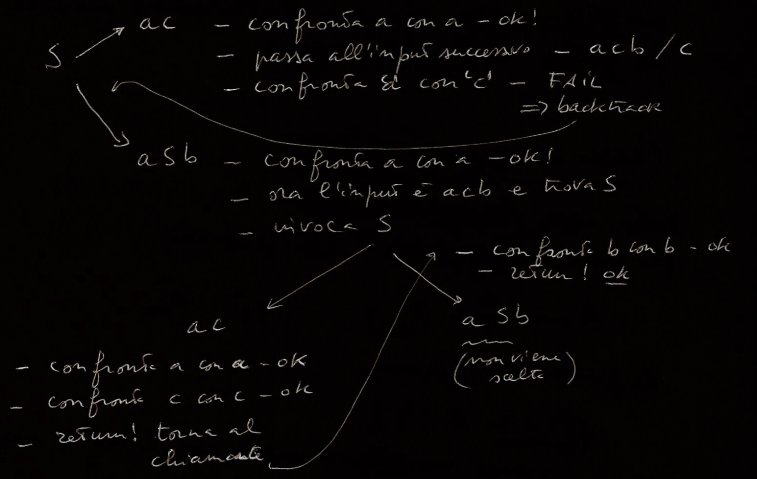
\includegraphics[width=10cm]{top-down-discesa-esempio.png}
    \end{center}

    \begin{center}
            \begin{tabular}{c c}
            \textbf{input} & \textbf{Stack delle chiamate} \\
            \\
            \underline{a} a c b & S \\
            \phantom{a}  & \underline{a} c \\
            \phantom{a} \underline{a} c b & c \textit{fail} \\
            \\
            \underline{a} a c b & S \\
            \phantom{a} & \underline{a} S b \\
            \phantom{a} \underline{a} c b & S b \\
            \phantom{a} & \underline{a} c b \\
            \phantom{a} \underline{c} b & \underline{c} b \\
            \underline{b} & b \\
            & \underline{ok} \\
            \end{tabular}
    \end{center}
}
Tuttavia il parser a discesa ricorsiva è \red{parecchio inefficiente a causa della sua natura nondeterminista}, vi è infatti la necessita nel peggiore dei casi di esplorare tutte le alternative

\teorema{
    Sia $w$ la lunghezza della stringa in inout, e sia $b$ il  massimo numero di produzioni per uno stesso nonterminale, allora la complessità computazionale di un parser a discesa riscorsiva nel caso peggiore è:
    \[
        O(b^{|w|})    
    \]
}

Per ovviare ovviare a questo problema di infecenza dobbiamo guidare la scelta della produzione per creare un parser top-down deterministico. Per farlo occorrono delle fuzioni ausiliarie

\section{Parser predittivo}
Il \textbf{parser predittivo} è un tipo parser deterministico (sotto alcune specifiche condizione che si vedranno più avanti), molto più efficiente in quanto non ha il backtracking, tuttavia per definirlo occorre prima definire delle funzioni ausiliarie
\subsection{First}
\dfn{First}{
    Data una grammatica libera $G \text{ e }\alpha\in(T\cup NT)^*$, di definisce \textbf{First($\alpha$)} come l'insieme dei terminali che possono stare in prima posizione in una stringa che si deriva da $\alpha$ 
    \begin{itemize}
        \item per $a \in T, a \in First(\alpha) \iff \alpha \implies^* a\beta \text{ per }\beta\in(T\cup NT)^*$
        \item inoltre $(\alpha \implies^*\epsilon)\implies \epsilon \in First(\alpha)$
    \end{itemize}
}
\osservazione{
    Sia la grammatica
    \[
        A \to \alpha_1 | \alpha_2       
        \]
        Se $First(\alpha_1)\cap First(\alpha_2) = \emptyset$ la scelta della produzione è deterministica
        }
Qui vi è riportato un esempietto:
\esempio{
    \[
        A\to aB|bC       
    \]
    Si ha che:
    \[
    \begin{array}{l}
        First(aB)= \{a\} \\
        First(bC) = \{b\} 
    \end{array}
    \]
    Pertanto abbiamo del determinismo con un solo carattere in lettura
}
\subsubsection{algoritmo per calcolare il first}
\begin{algorithm}[H]
    \SetAlgoNlRelativeSize{-1}
    \SetNlSty{textbf}{}{}
    \caption{First()}
    \KwIn{Una grammatica credo}
    \KwOut{bho}
    
        \For{$x\in T$}{
            $First(x)\gets \{x\}$\tcp*{un terminale è il primo elemento di se stesso}
        }
        \For{$X\in NT$}{
            $First(X)\gets \emptyset$\tcp*{per ogni x non terminale si inizializza il suo first a "0"}
        }
        \While{
            almeno un $First(X)$ può essere modificato in una iterazione\
        }{
            \ForEach{$x\to Y_1,\dots,Y_k$}{
                \ForEach{$i=1$\KwTo $k$}{
                    \tcp{se ciascuno di questi simboli $y_1,\dots,Y_{i-1}$ può derivare la stringa vuota $\epsilon$}
                    \If{$Y_1,\dots,Y_{i-1}\in N(G)$ }{
                        $First(X)\gets First(X)\cup (First(Y_i)\backslash\{\epsilon\})$\tcp*{allora è possibile aggiungere gli elementi di $FIRST(Y_i)$ a $FIRST(X)$ per la produzione $y_1,\dots,y_k$}
                    }
                    \tcp{Se invece uno dei simboli da $Y_1$ a $Y_{i-1}$ non è annullabile, si interrompe la ricerca per quella produzione, perché non possiamo "saltare" i simboli non annullabili per arrivare a $Y_i$}
                }
            }
        }
        \ForEach{
            $X\in N(G)$
        }{
            $First(X) = First(X)\cup\{\epsilon\}$\;
        }
\end{algorithm}

In generale per una stringa $\alpha$ si ha che:
\begin{itemize}
    \item Se \( \alpha = \varepsilon \), allora \( FIRST(\alpha) = \{\varepsilon\} \).
    \item Se \( \alpha = X \beta \) e \( X \notin N(G) \), allora \( FIRST(X \beta) = FIRST(X) \).
    \item Se \( \alpha = X \beta \) e \( X \in N(G) \), allora $FIRST(X \beta) = (FIRST(X) \setminus \{\varepsilon\}) \cup FIRST(\beta)$
\end{itemize}

In pratica se 
\[
    A\to \alpha_1 | \dots | \alpha_k    
\]
si ha che
\[
    First(A) = First (\alpha_1)\cup\dots\cup First(\alpha_k)   
\]

\esempio{
    Si ossrvi la seguente grammatica:
    \[
        \begin{array}{l}
            S\to Ab|c\\
            A\to aA|\epsilon
        \end{array}       
    \]

    \begin{align*}
        FIRST(S) &= FIRST(Ab) \cup FIRST(c) \\
                 &= (FIRST(A) \setminus \{\epsilon\}) \cup FIRST(b) \cup \{\epsilon\} \\
                 &= \{a\} \cup \{b\} \cup \{c\} = \{a, b, c\}
    \end{align*}
    
    \begin{align*}
        FIRST(A) &= FIRST(aA) \cup FIRST(\epsilon) \\
                 &= \{a\} \cup \{\epsilon\} = \{a, \epsilon\}
    \end{align*}
}
\subsection{Follow}
\dfn{Follow}{
    Data una grammatica libera \( G \) e \( A \in NT \), definiamo che \( Follow(A) \) è l'insieme dei terminali che possono comparire immediatamente a destra di \( A \) in una forma sentenziale.

    \begin{itemize}
        \item Per ogni \( a \in T \), \( a \in Follow(A) \) se \( S \Rightarrow^* \alpha A a \beta \) per qualche \( \alpha \) e \( \beta \in (T \cup NT)^* \).
        
        \item \( \$ \in Follow(A) \) se \( S \Rightarrow^* \alpha A \) (Poiché \( S \Rightarrow^* S \), allora \( \$ \in Follow(S) \) !)
    \end{itemize}
}
Riporto qui un esempio 
\esempio{
    \begin{align*}
        S &\rightarrow A b \mid c \\
        A &\rightarrow a A \mid \varepsilon
    \end{align*}
    
    \[
    Follow(S) = \{\$\} \quad Follow(A) = \{b\}
    \]
    
    \begin{itemize}
        \item \( S \Rightarrow^* S \)
        \item \( S \Rightarrow^* Ab \)
    \end{itemize}    
}
\subsubsection{algoritmo per calcolare il Follow}
\begin{algorithm}[H]
    \SetAlgoNlRelativeSize{-1}
    \SetNlSty{textbf}{}{}
    \caption{Follow()}
    \KwIn{Una grammatica credo}
    \KwOut{bho}
    
        \ForEach{$X\in NT$}{
            $First(X)\gets \emptyset$\tcp*{per ogni X non terminale si inizializza il suo first a "0"}
        }
        $Follow(S)\gets \{\$\}$\;
        \While{
            almeno un $Follow(X)$ può essere modificato in una iterazione
        }
        {
            \ForEach{$X\to\alpha Y\beta$}{
                $Follow(Y)\gets Follow(Y)\cup(First(\beta)\backslash \{\epsilon\})$\;
            }
            \ForEach{$X\to\alpha Y$}{
                \ForEach{$X\to \alpha \beta, \epsilon\in First(\beta)$}{
                    $Follow(Y)\gets Folloe
                    (Y)\cup Follow(X)$\;
                }
            }
        }
\end{algorithm}
in pratica, occorre cercare tutte le produzioni in cui $Y\in NT$ appare e, per ognuna di esse, applicare la 1 o la 2 sopra
\esempio{
    \begin{center}
    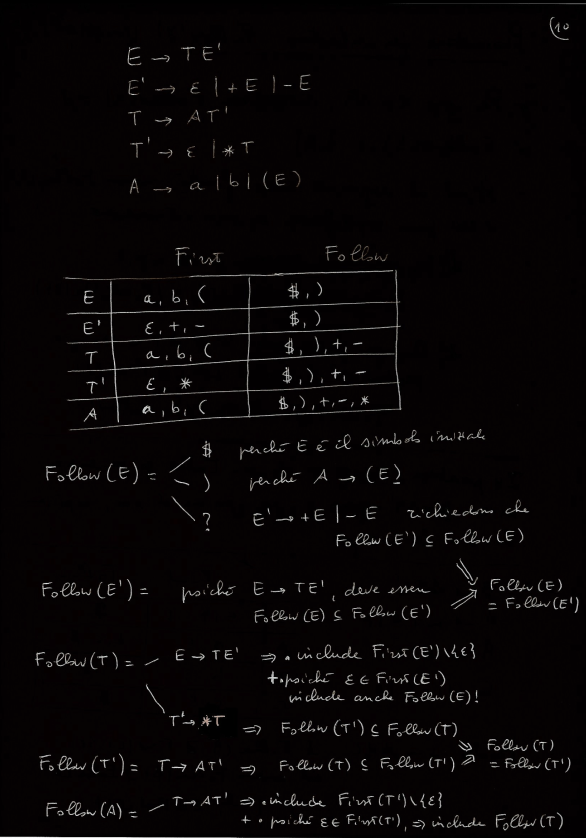
\includegraphics[width=10cm]{esempio-follow.png}
    \end{center}
}
Adesso che abbiamo introdotto i le procedure First e Follow occorre fare un passo in più per definire i parser

\subsection{Parser per linguaggi $LL(1)$}
\subsubsection{tabella di parsing LL(1)}
La tabella di parsing $LL(1)$ è una struttura di dati usata nei parser sintattici molto utili per risolvere il non determinismo. Questi parser leggono l'input da sinistra a destra (da qui il primo "L" di "LL"), costruendo una derivazione sinistra, o leftmost (da qui il secondo "L") e usano un solo simbolo di lookahead (da cui il "(1)").

Questa tabella è formata da una \textbf{matrice bidimensionale $M$} che è formata da:
\begin{itemize}
    \item \textbf{righe}: non-terminali
    \item \textbf{colonne}: terminali (incluso \$)
    \item \textbf{casella} $(A, a)$: $M[A, a]$ contiene le produzioni che possono essere scelte dal parser mentre tenta di espandere $A$ e l'input corrente è $a$.
\end{itemize}

Se ogni casella contiene \red{al più una produzione}, allora il parser è \red{deterministico}!


Per riempire la tabella occorre procedere in questo modo:

Per ogni produzione $A \rightarrow \alpha$:
\begin{enumerate}
    \item per ogni $a \in T$ e $a \in \text{First}(\alpha)$, inserisci $A \rightarrow \alpha$ nella casella $M[A, a]$
    \item se $\varepsilon \in \text{First}(\alpha)$, inserisci $A \rightarrow \alpha$ in tutte le caselle $M[A, x]$ per $x \in \text{Follow}(A)$ (x può essere \$)
\end{enumerate}

Ogni casella vuota, dopo aver elaborato tutte le produzioni, è un errore (cioè la funzione ricorsiva chiama `fail')

\subsubsection{grammatica $LL(1)$}

\dfn{grammatica $LL(1)$}{
    Una grammatica si definisce $LL(1)$ sse ogni casella della tabella di parsing $LL(1)$ contirne al più una produzione, ovvero non presenta conflitti
}

Si ha che \red{se $G=LL(1)$ allora il parser è predittivo e deterministico}, questo perché il parser ricostruisce l'albero di derivazione per l'input $w$, in modo top-down, predicendo quale produzione usare (tra le molte possibili) guardando il prossimo carattere dell'input

\teorema{
    $G$ è $LL(1)$ sse per ogni coppia di produzioni distinte con la stessa testa 
    \[
        A\to \alpha|\beta       
    \]
    si ha che \begin{enumerate}
        \item $First(\alpha)\cap First(\beta)=\emptyset$
        \item \begin{enumerate}
            \item $(\epsilon\in First(\alpha))\implies (First(\beta)\cap Follow(A) = \emptyset)$
            \item $(\epsilon\in First(\beta))\implies (First(\alpha)\cap Follow(A) = \emptyset)$
        \end{enumerate}
    \end{enumerate}
}
\dimostrazione{
    Se sono soddisfatte le condizione 1 e 2 per ogni coppia di produzioni distinte con medesima testa allora la tabella di parsing $LL(1)$ contiene al più una prodizone in ogni cassella. 
    Ma vale anche viceversa!
}

\subsubsection{Linguaggio $LL(1)$}
\dfn{Linguaggio $LL(1)$}{
    Un linguaggio si definisce $LL(1) \iff \exists G' \text{ grammatica } = LL(1)$ che lo genera 
}
\esempio{
    Sia $G$ la segunete grammatica:
    \[
        \begin{array}{l}
            S\to A|B\\
            A \to ab|cd\\
            B\to ad|cb
        \end{array}       
    \]
    Si può notare che $G$ non è $LL(1)$ dato che $S\to A|B$ e 
    \[
        \begin{array}{l}
            First(A) = \{a,c\}\\
            First(B) = \{a,c\}\\
            First(A)\cap First(B) = \{a,c\}
        \end{array}
    \]
    Dal teorema sopra fornito si può dimostrare che non è $LL(1)$\\
    Tuttavia si può manipolarla per farla diventare $LL(1)$, quindi espando $S$:
    \[
        S\to ab|cd|ad|cb    
    \]
    \[
        \begin{array}{l}
            S\to aT|cT'\\
            T\to b|d\\
            T'\to b|d
        \end{array}    
    \]
    Poi osservo che $T$ e $T'$ sono identici, sia quindi $G'$ la nuova grammatica:
    \[
        \begin{array}{l}
            S\to aT|cT  \\
            T\to b|d
        \end{array}
    \]
    Si può dimostrare che è $LL(1)$, pertanto, per la definizione di linguaggio $LL(1)$ e nonostante $G$ non sia $LL(1)$, si ha che $L(G) =\{ ab,cd,ad,cb\}$ è un linguaggio $LL(1)$ perché $G'$ che lo genera è una grammatica $LL(1)$  
    }

    \teorema{
        Ogni linguaggio regolare è generabile da una grammatica $G$ di classe $LL(1)$
    }
    \dimostrazione{
        Sia $L$ un linguaggio regolare, allora $\exists \text{ DFA }M=(Q,\Sigma , \delta, q_0, F):L=[M]$.

        A partira da $M$ si può costruire una grammatica regolare $G=(NT,T,S,R)$ basata sul seguente automa $M$:
        \begin{itemize}
            \item $NT=\{[q]|q\in Q\}$, cioè un non terminale per ogni stato $q$
            \item $T= \Sigma$ cioè un terminale per ogni simbolo dell'alfabeto
            \item $S=[q_0]$ simbolo iniziale lo stato iniziale
            \item $R$ (insieme delle produzioni) è definito come:
            \begin{itemize}
                \item se $\delta (q,a) = q'$, allora $[q]\to a[q']\in R$
                
                Infatti $\delta (q,a) = q'$ vuol dire che l'automa si trova allo stato $q$ e legge in input $a$ allora arriverà allo stato $q'$, che viene "tradotto" nella grammatica $[q]\to a[q']$ che corrisponde ad una produzione in cui il non terminale $[q]$ produce il terminale $a$ e il non terminale $[q']$, per passare al non terminale $[q']$ occorre, infatti, fare match con $a$
                \item se $q\in F$, allora $[q]\to \epsilon\in R$
            \end{itemize}
        \end{itemize}

        Poi che $M$ è deterministico, \( \forall q \in Q \forall a \in \Sigma \quad \exists! q'. q \xrightarrow{a} q' \), cioè \( [q] \) avrà una sola produzione \( [q] \to a[q'] \) che "inizia" per \( a \) e dato che se \( q \) è finale, allora \( [q] \to \epsilon \) è applicabile solo per i \(\text{Follow}([q]) = \{\$\} \implies \text{ nessun conflitto}\), dato che nessuna produzione genera $\$$, si ha che $G$ è $LL(1)$
    }
    \esempio{
        \begin{center}
            \begin{tikzpicture}[shorten >=1pt,node distance=2cm,on grid,auto] 
              \node[state,initial] (q_0)   {$q_0$}; 
              \node[state,accepting] (q_1) [right=of q_0] {$q_1$}; 
              \path[->] 
                (q_0) edge [loop above] node {a} ()
                      edge [bend left]  node {a} (q_1)
                (q_1) edge [bend left]  node {a} (q_0);
            \end{tikzpicture}
        \end{center} 
            Le produzioni corrispondenti sono:
                \begin{center}
                    \begin{tabular}{ ll }
                        $[q_0] \to a[q_1] \mid a[q_0]$\\
                        $[q_1] \to a[q_0] \mid \epsilon$ \\  

                \end{tabular}
            \end{center}
            
               
            
            La grammatica \( G \) è \( LL(1) \), perché:
            \[
                \text{First}(a[q_0]) \cap \text{First}(\epsilon) = \emptyset, \quad \text{First}(a[q_1]) \cap \text{First}(\epsilon) = \emptyset
            \]
    }
    
    Riporto qui un esempio di tabella di parsing $LL(1)$:
    \esempio{
        Sia $G$ la seguente grammatica:
        \[
            \begin{array}{l}
                E \to T E' \\
                E' \to \varepsilon \, | \, + T E' \, | \, - T E' \\
                T \to A T' \\
                T' \to \varepsilon \, | \, \ast T \\
                A \to a \, | \, b \, | \, (E)
                
            \end{array}       
    \]
    
    Si può costruire la seguente tabella di First e Follow:
    \[
        \begin{array}{|c|c|c|}
            \hline
            \text{Produzione} & \text{First} & \text{Follow} \\
            \hline
            E & a, b, ( & \$, ) \\
            E' & +, -, \varepsilon & \$, ) \\
            T & a, b, ( & +, -, \$, ) \\
            T' & \ast, \varepsilon & +, -, \$, ) \\
            A & a, b, ( & \ast, +, -, \$, ) \\
            \hline
        \end{array}
        \]
        
        Ed ecco a voi la tabella di parsing:
        \[
            \begin{array}{|c|c|c|c|c|c|c|}
                \hline
                & a & b & ( & + & \ast & \$ \\
                \hline
                E & E \to T E' & E \to T E' & E \to T E' &  &  &  \\
                E' &  &  &  & E' \to + T E' & E' \to - T E' & E' \to \varepsilon \\
                T & T \to A T' & T \to A T' & T \to A T' &  &  &  \\
                T' &  &  &  & T' \to \varepsilon & T' \to \ast T & T' \to \varepsilon \\
                A & A \to a & A \to b & A \to (E) &  &  &  \\
                \hline
            \end{array}
            \]
            
            \begin{center}
                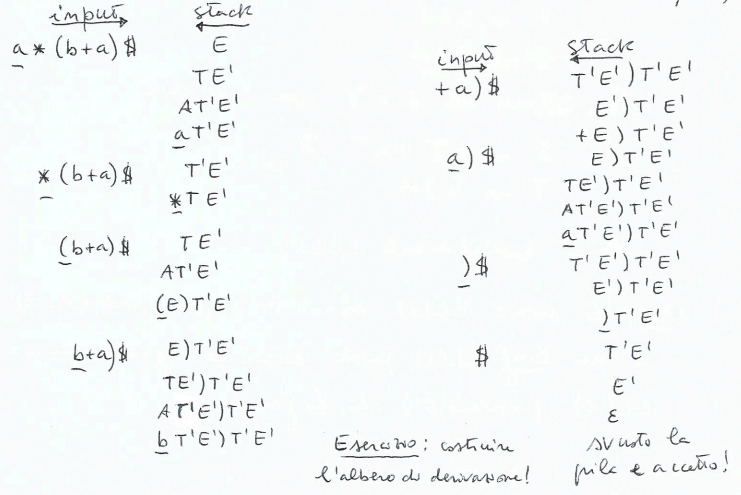
\includegraphics[width=7cm]{parser-con-pila.png}
            \end{center}   
}

\subsubsection{Algoritmo Per il calcolo di un parser $LL(1)$}

\begin{algorithm}
    \caption{Parser $LL(1)$}
    \KwIn{Stringa $w$}
    \KwOut{Niente}

    $Pila\gets S\$$\tcp*{cima della pila a sinistra}
    $X\gets S$ \tcp*{top della pila}
    \tcp{lettura in input}
    $input \gets w\$$\;
    $i_c = \text{ primo carattere dell'input}$\;
    \tcp{viene eseguito il ciclo While finché la pila non è vuota o l'input non è stato consumato}
    \While{$X\neq \$$}{
        \If{$X$ è un terminale}{
            \tcp{si controlla se $X$ fa "match" con $i_c$}
            \If{$X = i_c$}{
                Pop $X$ dalla pila\tcp*{rimuovo $X$ dalla pila}
                avanza $i_c$ sull'input\;
            }
            \Else{
                Errore()\tcp*{no match}
            }
        }
        \Else{
            \tcp{se nella tabella di Parsing $M$ esiste una regola $X\to Y_1, \dots, Y_n$}
            \If{$M[X,i_c] = X\to Y_1, \dots, Y_n$}{
                Pop $X$ dalla pila\;
                Push $Y_1, \dots, Y_n$ sulla pila \tcp*{mette sulla pila i simboli $Y_1, \dots, Y_n$ con $Y_1$ in cima}
                In output la produzione $X\to Y_1, \dots, Y_n$\; 
            }
            \Else{
                Errore ()\tcp*{se non esiste una regola  in $M[X,i_c]$ si genera un errore, viene definito caso "bianco"} 
            }
            $X\gets$ top della pila\tcp*{Aggiorna $X$ con il nuovo simbolo in cima alla pila}
        }
    }
    \If{$i_c\neq \$$}{
        Errore()\tcp*{pila svuotata ma vi è ancora dell'input da leggere}
    }
\end{algorithm}



Un altro esempio:
\esempio{
    Sia $G$ la seguente grammatica:
    \[
    \begin{aligned}
        S &\to aAB \, | \, bS \\
        A &\to a \\
        B &\to b
    \end{aligned}
    \]
    Che genera il seguente linguaggio
    \[    
        L(G) = L\big(b^*aab\big)
    \]
    Si ha che questa grammatica \(G\) è LL(1), perché:
    \[
        First(aAB) \cap First(bS) = \varnothing, \quad \{a\} \cap \{b\} = \varnothing
    \]

    Si può prosegure con la tabella First e follow:
    \[
        \begin{array}{|c|c|c|}
        \hline
        Simbolo & First & Follow \\
        \hline
        S & a, b& \$ \\
        A & a& b \\
        B & b& \$ \\
        \hline
        \end{array}
    \]
    Da cui si può costruire la seguente tabella di parsing:
    \[
        \begin{array}{|c|c|c|c|}
        \hline
        & a & b & \$ \\
        \hline
        S & S \to aAB & S \to bS &  \\
        A & A \to a &  &  \\
        B &  & B \to b &  \\
        \hline
        \end{array}
    \]
    
    Viene qui descritto il funzionamento del parser con pila con diversi input:
    \begin{center}
    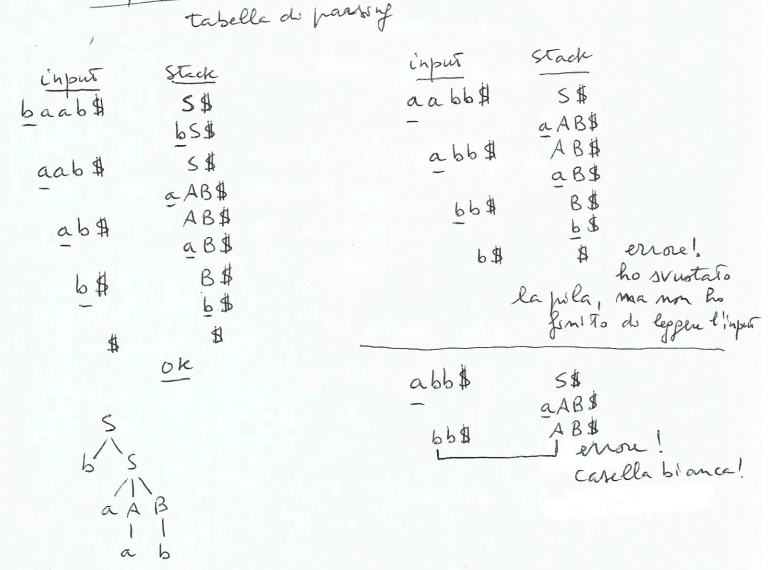
\includegraphics[width=10cm]{parser-pila-2.png}
    \end{center}


}

\subsection{Parser per linguaggi $LL(K)$}
\subsubsection{grammatiche $LL(K)$}
Le grammatiche $LL(k)$ sono "un'estensione" del concetto di grammatiche $LL(1)$, dove il parser ha la capacità di guardare in avanti fino a $k$ simboli per determinare le scelte di parsing

Per questi tipi di grammatica gli insiemi $First \text{ e }Follow$ assumo significati diversi rispetto a alle grammatiche $LL(K)$
\dfn{First $LL(K)$}{
    L'insieme \(First_k(\alpha)\) contiene tutte le stringhe di lunghezza \( k \) o minore derivabili dall'inizio di una produzione con \( \alpha \), in particolare
    $w\in First_k(\alpha) \iff \alpha \implies^{*}w\beta \text{ con } |w|=k,w\in T^{*}, \beta\in (T\cup NT)^* \text{ oppure }  \alpha \Rightarrow^* w  \text{ con } |w| \leq k \text{ e }  w \in T^* $
}
\dfn{Follow $LL(K)$}{
    L'insieme Follow\(_k(A)\) definisce quali stringhe possono apparire immediatamente dopo un simbolo non terminale \( A \) in una derivazione a partire dal simbolo iniziale \( S \). In particolare:
    \( w \in \text{Follow}_k(A) \) se \( S \Rightarrow^* \alpha A w \beta \) con \( |w| = k \), \( w \in T^* \), e \( \alpha, \beta \in (T \cup NT)^* \), oppure, \( S \Rightarrow^* \alpha A w \) con \( |w| \leq k \) e \( w \in T^* \).
}

\subsubsection{Tabella di Parsing $LL(K)$}
\begin{itemize}
    \item \textbf{Righe}: non terminali.
    \item \textbf{Colonne}: $\{ w \in T^* \mid |w| \leq k \}$ (solo quelle necessarie).
\end{itemize}

\noindent Per ogni produzione $A \to \alpha$, la tabella $M[A, w]$ contiene:
\begin{itemize}
    \item $A \to \alpha$, per ogni $w \in \text{First}_k(\alpha)$ ($w \neq \varepsilon$);
    \item $w \in \text{Follow}_k(A)$ se $\varepsilon \in \text{First}_k(\alpha)$.
\end{itemize}

\noindent Ogni entrata/casella contiene al più una produzione. Se non esistono $w_1$ e $w_2$ tali che $w_1$ prefisso di $w_2$ con le due entrate corrispondenti su una riga entrambe riempite, allora $G$ è una grammatica LL(k).

\vspace{1em}
\noindent \textbf{Nota Bene:} 
Le colonne sono tante quante sono le stringhe $w$ che appartengono a $\text{First}_k(\alpha)$ per $A \to \alpha$ o a $\text{Follow}_k(A)$ per $A \to \alpha$. Questo va verificato per tutte le produzioni:
\[
w \in \text{First}_k(\alpha).
\]

\esempio{
    Sia $G$ la seguente grammatica
    \[
        S\to aSb\mid ab\mid c
    \]
    Si ha che $L(G) = \{a^nb^n\mid n\geq 1\}\cup\{a^ncb^n\mid n\geq 0\}$, inoltre:
    \begin{itemize}
        \item $First_2(aSb) =\{aa,ac\}$
        \item $First_2(ab) =\{ab\}$
        \item $First_2(c) = \{c\}$
    \end{itemize}

    Si può dimostrare che $G$ è $LL(2)$ dato che:
    \begin{itemize}
        \item $First_2(aSb)\cap First_2(ab)=\varnothing$
        \item $First_2(aSb)\cap First_2(ab)=\varnothing$
        \item $First_2(aSb)\cap First_2(ab)=\varnothing$
    \end{itemize}
    Da cui si può ricavare la tabella di parsing:
    \[
        \begin{array}{|c|c|c|c|c|}
        \hline
        Simbolo & aa & ab & ac & c \\
        \hline
        S & S \to aSb& S\to ab&S\to aSb & S\to c \\
        \hline
        \end{array}
    \]

}
        
\teorema{
    \begin{itemize}
        \item Una grammatica ricorsiva sinistra non è $LL(K)$ per nessun $K$
        \item Una grammatica ambigua non è $LL(K)$
        \item Se $G$ è $LL(K)$ per qualche $k$, allora $G$ non è ambigua 
        \item Se $G$ è $LL(K)$, allora $L(G)$ è libero deterministico
        \item esiste $L$ libero deterministico tale che non esiste G di classe $LL(K)$ per nessun $K$, tale che $L=L(G)$
    \end{itemize}
}


Viene qui riportato il funzionamento del parser con pila:
\subsubsection{Linguaggio $LL(K)$}

\dfn{Linguaggio $LL(K)$}{
    un linguaggio $L$ è di classe $LL(K)$ se $G$ di classe $LL(K)$ tale che $L=L(G)$
}

\teorema{
    $\forall k\geq 0$, la classe dei linguaggi $LL(K)$ contiene strettamente la classe dei linguaggi $LL(K)$
}
\osservazione{
    $\forall k\geq 0,$ la classe dei linguaggi $LL(K+1)$ contiene strettamente la classe dei linguaggi $LL(K)$
    \begin{center}
    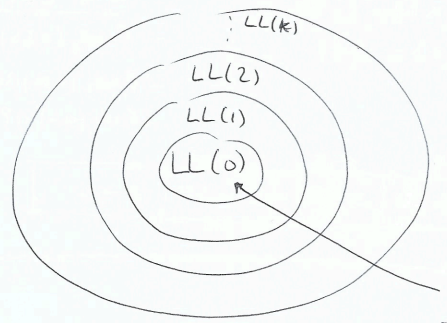
\includegraphics[width=10cm]{gerarchia-dei-linguaggi.png}
    \end{center}
    Si ha che: $(\forall A \in NT, \quad \exists! \alpha \in (T \cup NT)^*, \quad A \to \alpha \implies G \text{ è } LL(0))\implies L(G) = \{w\}$ ovvero una sola parola al massimo
}

\red{Nella pratica tuttavia si usano solo $LL(1)$}, spesso la si può manipolare trasformandola in $LL(1)$

\esempio{
    \[
      \begin{array}{l}
        S\to Asb\mid ab\mid c\\
      \end{array}       
    \]
    $G$ è un $LL(2)$ ma non $LL(1)$
    Si fattorizza
    \[
    \begin{array}{l}
        S\to aT|c\\
        T\to Sb|b
    \end{array}
    \]
    Ottenuta fattorizzando $G$ è $LL(1)$ infatti:
    \begin{itemize}
        \item $First(aT)\cap First(c)=\varnothing$
        \item $First(Sb)\cap First(b)=\varnothing$
    \end{itemize}
    Si ha che $L = \{a^n b^n\mid n\geq 1\}\cup \{a^ncb^n\mid n\geq 0\}$ è un linguaggio di classe $LL(1)$ perché $G'$ è $LL(1)$
}
\subsubsection{Casi speciali}
Sia 
\[
    L= \{a^i b^j | i\geq j\} \text{ è libero deterministico}    
\]
Ma non è $LL(K)$ per nessun $K$!

Adesso, mostriamo una grammatica per $L$ e dimostriamo che non è LL(K) per nessun $K$.
Sia $G$ la seguente grammatica:
\[
    \begin{array}{l}
        S\to aS|B\\
        B\to aBb|\epsilon    
    \end{array}
\]

\begin{center}
    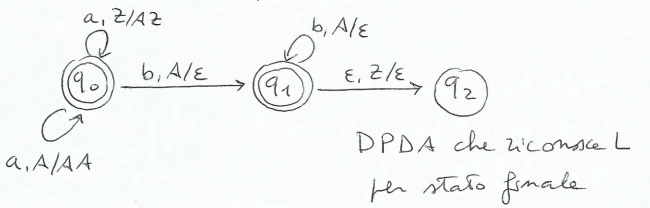
\includegraphics[width=10cm]{l-libero-deterministico-non-ll-k.png}
\end{center}

Sia $G$ una grammatica libero per $L$
\[
    S\to aS\mid B \\
    B\to aBb \mid \epsilon    
\]
e poniamo $L=L(G)$

%! NON HO CAPITO CAZZO

Per scegliere tra $S\to aS$ e $S\to B$ dovrei leggere fino in fondo l'input per sapere quante $b$ in meno di $a$ ci sono nella stringa! Allora $G$ non può essere $LL(k)$ per nessun $k$. Infatti quanto possa essere grande il $K$ posso trovare una stringa più lunga che richiede di leggere più di $k$ simboli di lookahead

Non è tuttavia possibile alcuna $G'$ e $k$ tali che
\[
    L(G') = L \text{ e }G'\in L(K)    
\]
La dimostrazione non verrà illustrata 

\chapter{Bottom up parser}

Il \textbf{parser bottom up} è un tipo di analizzatore sintattico che che costruisce l'albero di derivazione partendo dalle foglie, viene anche detto \textbf{Shift-Reduce} in quanto possiede due operazioni fondamentali:
\begin{itemize}
    \item \texttt{Shift}: un simbolo terminale viene spostato dall'input alla pila 
    \item \texttt{Reduce}: una serie di simboli (terminali e non terminali) sulla cima della pila corrisponde al "reverse" di una parte destra di una produzione, ovvero:
    \[
        A\to\alpha \in R - \alpha^R \text{ sulla pila}
    \]
    La stringa $\alpha^T$ viene rimossa dalla pila e sostituita con $A$, quindi $\alpha$ viene ridotta ad $A$
\end{itemize}

Possono essere di diversi tipi

\section{Parser shift-reduce nondeterministico}
\begin{algorithm}
    \caption{Parser shift-reduce nondeterministico}
    \KwIn{Una grammatica libera $G$ con simbolo iniziale $S$ e una stringa $w\in T^*$}
    \KwOut{Una stringa $w\in T^*$}

    Inizializziamo la pila a $\$$\;
    Inizializziamo l'input con $w\$$\;
    usaimo il $PDA$ seguente per trovare la derivazione per $w\$$:
    \[
        M=(T, \{q\},\underbracket{T\cup NT \cup \{\$\}}_{\Gamma: \text{ovvero i simboli sulla pila}}, \delta, \varnothing)
    \]
    Dove:
    \begin{enumerate}
        \item $(q,aX)\in \delta (q,a,X)\forall A\in T\forall X\Gamma\quad \text{SHIFT}$
        \item $(q,A)\in\delta(q,\epsilon, \alpha^R)$ se $A\in \alpha\in R\quad \text{REDUCE}$
        \item $(q,\epsilon)\in \delta(q,\$,S\$)\quad \text{accept}$
    \end{enumerate}\;
    ogni volta che facciamo "reduce", forniamo in output la produzione usata\;
    alla fine, $S\$$ sulla pila, con $\$$ in input $\implies$ accettiamo\;
\end{algorithm}

\nt{
    generalizzazione della def. di $PDA$ dove non si consuma solo il top della pila, ma una serie di caratteri contigui a caminciare dal top
}

\esempio{
    Sia la seguente grammatica
    \[
        \begin{array}{l}
            E\to T\mid T+E \mid T-E\\
            T\to A\mid A*T\\
            A\to a\mid b\mid (E)
        \end{array}
    \]
    \[
        \begin{array}{|c|l|l|l|l|}
        \hline
        \textbf{N.} & \textbf{Pila} & \textbf{Input} & \textbf{Azione} & \textbf{Output} \\ \hline
        1  & \$                  & a+b*b\$              & Shift         &                 \\ \hline
        2  & \$a                & +b*b\$               & Reduce        & A \to a         \\ \hline
        3  & \$A                & +b*b\$               & Reduce        & T \to A         \\ \hline
        4  & \$T                & +b*b\$               & Shift         &                 \\ \hline
        5  & \$T+               & b*b\$                & Shift         &                 \\ \hline
        6  & \$T+b              & *b\$                 & Reduce        & A \to b         \\ \hline
        7  & \$T+A              & *b\$                 & Shift         &                 \\ \hline
        8  & \$T+A*             & b\$                  & Shift         &                 \\ \hline
        9  & \$T+A*b            & \$                   & Reduce        & A \to b         \\ \hline
        10 & \$T+A*B            & \$                   & Reduce        & T \to A * T     \\ \hline
        11 & \$T+A*T            & \$                   & Reduce        & E \to T + T     \\ \hline
        12 & \$E                & \$                   & Reduce        & E \to T + T     \\ \hline
        13 & \$E                & \$                   & Accept        &                 \\ \hline
        \end{array}
    \]

    Si ha che:
    \[
        E\implies T+E\implies T+T \implies T + A* T \implies T+A*A \implies T + A * b \implies T + b * b \implies A + b*b  \implies a + b*b
    \]

    Il cui albero è:
    \begin{center}
        \begin{tikzpicture}
            \Tree [
                .E
                [
                    .T
                    [
                        .A
                        [
                            .a
                        ]
                    ]
                ]
                [
                    .+
                ]
                [
                    .E
                    [
                        .T
                        [
                            .A
                            [
                                .b
                            ]
                        ]
                        [
                            .*
                        ]
                        [
                            .T
                            [
                                .A
                                [
                                    .b
                                ]
                            ]
                        ]
                    ]
                ]
            ]
        \end{tikzpicture}
    \end{center}
    
    Le cui proprietà sono:
    \begin{center}
        \item Costruzione dell'albero di derivazione \textit{bottom-up}    
        \item Derivazione canonica a destra a rovescio
        \item forte non-determinismo:
        \begin{itemize}
            \item \textbf{conflitti shift-reduce}:
            \begin{itemize}
                \item $\$a \quad +b*b\$ \quad \text{shift}$
                \item $\$ a+ \quad b*b \$$
            \end{itemize}
            \item \textbf{Conflitti reduce-reduce}
            \begin{itemize}
                \item $\$T+A*T\quad\$$ reduce $E\to T$
                \item $\$T+A*E\quad\$$
            \end{itemize}
        \end{itemize}
    \end{center}
}

\nt{Si noti quindi che questo tipo parser genera moltissimi confilitti, in diverse sistuazioni era appunto possibile scegliere strade che non portano a riconoscere la stringa. F}

Per "risolvere" tale nondeterminismo occorre fornire al PDA una tabella parsing (struttura di controllo) che "aiuti" a scegliere l'azione giusta, ed è grazie all'uso di questa che nascono i cosiddetti \textbf{parser LR}

\section{Parser LR}
\dfn{Parser LR}{
    Il \textbf{parser LR} è un tipo di analizzatore sintattico che utilizza un approccio bottom-up per analizzare un input e verificare se appartiene al linguaggio generato da una grammatica libera. Il termine LR indica che:
    \begin{itemize}
        \item L: sta per \textit{left-to-right}: l'analisi dell'input avviene da sinistra a destra
        \item R: sta per \textit{Rightmost derivation}: l'analisi ricostruisce una derivazione più a destra in senso inverso
    \end{itemize}
}

Presento, qui uno schema bellino bellino:

%TODO DA FARE QUESTA GIGAMINCHIATA
\begin{center}
    \begin{tikzpicture}
        % Input
        \node at (-2.5, 3.5) {Input:};
        \node[stack] (input1) at (-1,0) {$a_1$};
        \node[stack, right of=input1] (input2) {$a_2$};



        % \node[stack] (input2) at (0,1) {$a_2$};
        % \node[stack] (dots) at (1, 2) {$\dots$};
        % \node[stack] (inputn) at (2,3) {$a_i$};
        % \node[stack] (end) at (3, 4) {$\dots$};
        % \node[stack] (end) at (4, 5) {$a_k$};
        % \node[stack] (end) at (5, 6) {$\$$};
    
        % Parser LR block
        \node[block] (parserLR) at (0,1.5) {Parser LR};
    
        % Output
        \node at (4.5, 1.5) {Output:};
        \node[align=center] (output) at (6.7,1.5) {Derivazione \\ \textit{rightmost} \\ = albero di derivazione};
    
        % Parsing Table
        \node[block] (table) at (0,-1.5) {Tabella di Parsing $M$ \\ \vspace{0.2cm} \textbf{Azione} (Shift/Reduce) \\ sui Terminali \\ \textbf{GOTO} sui Nonterminali};
    
        % Stack
        \node at (-4.2, 1.5) {Pila:};
        \node[stack] (stack0) at (-3.5,1.5) {$S_0$};
        \node[stack] (stackdots) at (-3.5,0.7) {$\vdots$};
        \node[stack] (stackn) at (-3.5,-0.1) {$S_m$};
    
        \node at (-4.2, -1.5) {Pila simboli:};
        \node[stack] (symbol0) at (-3.5,-1.5) {$X_0$};
        \node[stack] (symboldots) at (-3.5,-2.3) {$\vdots$};
        \node[stack] (symboln) at (-3.5,-3.1) {$X_m$};
    
        % Arrows
        \draw[arrow] (input1.south) -- (parserLR.north);
        \draw[arrow] (parserLR.south) -- (table.north) node[midway,right] {consulta};
        \draw[arrow] (parserLR.east) -- (output.west);
    
        \draw[arrow] (stack0.east) ++(0.2,0) -- (parserLR.west);
        \draw[arrow] (symbol0.east) ++(0.2,0) -- (parserLR.west);
    
        % DFA note
        \node[align=center] at (5,-2) {Generata a partire \\ da un DFA \\ (Automa canonico \\ degli stati \\ \textit{viabili})};
    \end{tikzpicture}    
\end{center}

dove una configurazione di tale parser è:
\[
    (s_0, \dots, s_n, x_1 \dots x_m, a_1 \dots a_k \$)
\]

\nt{
    $x_1 \dots x_m a_1 \dots a_k$ è una stringa intermedia della derivazione canonica destra
}
\subsection{Funzionamento del parsing LR}
il parser LR funzione nel seguente modo:
\begin{enumerate}
    \item Legge lo stato nel top della pila $s_n$ e il simbolo corrente dell'input $a_i$
    \item consulta la tabella di parsing LR $M[s_n, a_i]$
    \begin{itemize}
        \item Se $M[s_n, a_i] = \text{shift}\; s$, allora la nuova configurazione è:
        \[
            (s_0\dots s_n \underline{s}\;, x_1 \dots x_n \underline{a_i}, a_{i+1} \dots a_k \$)
        \]
        \item Se $M[s_n, a_i]= \underline{\text{reduce } A\to B}$, allora la nuova configurazione è
        
        \[
            (s_0 \dots s_{n-r} \underline{s}, x_1 \dots x_{m-r}A, a_i\dots a_k \$)
        \]
        Dove $r=|\beta|$ e $M[s_{n-r}, A]=goto \; \underline{s}$

        Cioè fa tre passi:
        \begin{enumerate}
            \item faccio "pop" di r elementi dai 2 stack
            \item metto A in cima alla pila dei simboli
            \item calcolo il nuovo stato top, guardando 
            \[
                M[s_{n-r}, A] = goto\; s \text{ e metto }s\text{ in cima alla pila degli stati}
            \]
        \end{enumerate}
        \item se $M[s_n, a_i] = accept \implies$ fine!
        \item se $M[s_n, a_i] = "bianco" \implies$ errore!
    \end{itemize}
\end{enumerate}
\esempio{
    Sia $G$ la seguente grammatica:
    \[
        \begin{array}{l}
            S'\to S\\
            Senza\to (S)\\
            S\to ()
        \end{array}
    \]

    % Tabella di Parsing LR(0)
    Assumendo che siamo già forniti di questa \textbf{Tabella di Parsing}

    \[
    \begin{array}{|c|ccc|c|}
    \hline
    \text{Stato} & \multicolumn{3}{c|}{\textbf{Azione}} & \textbf{Goto} \\
    \cline{2-4}
    & ( & ) & \$ & S \\
    \hline
    0 & S2 &  &  & g1 \\
    1 &  &  & \text{Accept} & g3 \\
    2 & S2 & S5 &  &  \\
    3 &  & S4 &  &  \\
    4 & r2 & r2 & r2 &  \\
    5 & r3 & r3 & r3 &  \\
    \hline
    \end{array}
    \]

    \vspace{0.5cm}

    % Seconda tabella: Stato della pila, input, azione e output
    \noindent\textbf{Esecuzione del Parsing}


    \[
        \begin{array}{|l|l|l|c|l|}
        \hline
        \text{Stato della pila} & \text{Stack simboli} & \text{Input} & \text{Azione} & \text{Output} \\
        \hline
        (0 & \varepsilon & (())\$ & S2 & - \\
        (0,2 & ( & ())\$ & S2 & - \\
        (0,2,2 & (( & ))\$ & S5 & - \\
        (0,2,2,5 & (() & )\$ & r3 & S \to () \\
        (0,2,3 & (S & )\$ & S4 & - \\
        (0,2,3,4 & (S) & \$ & r2 & S \to (S) \\
        (0,1 & S & \$ & Accept & - \\
        \hline
        \end{array}
    \]
}

Tuttavia una domanda lecita è come si fa trovare questa tabella di parsing, bhe prima di presentarla occorre definire un automa dei prefissi variabili

\subsection{DFA a prefissi variabili}

\dfn{prefisso variabile}{
    un prefisso variabile è una stringa $\in (T\cup NT)^*$ che può apparire sulla pila di un parser bottom-up per una computazione che accetta un input
}

\dfn{prefisso viabile su una grammatica $G$ libera }{
    si definisce prefisso viabile su una grammatica $G$ libera una stringa $\gamma\in(T\cup NT)^* $ sse esiste una derivazione rightmost
    \[
        S\implies^* \delta A y \implies \delta \alpha \beta y = \gamma \beta y
    \]
    Dove: 
    \begin{itemize}
        \item $y\in T^*$
        \item $\delta\in (T\cup NT)^*$
        \item esiste una produzione $A\to \alpha \beta$
    \end{itemize}

    Inoltre $S$ è un prefisso variabile per definizione
}
\dfn{prefisso variabile completo e maniglia}{
    un prefisso viabile si dice completo se $\beta=\epsilon$, in tal caso $\alpha$ è detta maniglia per $\gamma y$
}
Dopo sta sborodolata di definizioni si possa al teorema che lega i prefissi variabili con i DFA:
\thm{}{
    Data $G$ libera, i prefissi viabili di $G$ costituiscono un linguaggio regolare e può essere descritto con un DFA. detto \textbf{DFA a prefissi viabili o automa canonico LR(0)}
}

Pertanto si ha questo corollario
\begin{corollary}
Il parser può consultare il DFA dei prefissi viabili (ovvero la tabella di parsing) per decidere cosa fare:
\begin{itemize}
    \item se la pila contiene un prefisso viabile completo il parser riduce
    \item se la pila contiene un prefisso viabile incompleto, allora il parser shifta
    \item se la pila non contiene un prefisso viabile, allora viene dato un errore
\end{itemize}  
\end{corollary}
In base a come è fatto questo DFA (che eventualmente può usare informazioni di look-ahead e dei follow) il parser può risultare deterministico o meno

Si noti, inoltre la seguente osservazione
\nt{
    si può dimostrare che un prefisso di un prefisso viabile è un prefisso viabile pertanto si ha che non è necessario ripartire da capo quando viene modificata la pila (ovvero il parser)
}

infatti la pila viene modificata in due modi:
\begin{enumerate}
    \item \textbf{shift}: la pila passa da $\$ \gamma$ a $\$\gamma x$. Dato che si trova in uno stato $s$ dopo aver elaborato un $\$\gamma$, occorre soltanto far ripartire il DFA da $S$ con input $x$
    \item la pila passa da $\$ \gamma\alpha$ a $\$ \gamma A$. Dato che si trova in uno stato $s$ dopo aver elaborato $\$ \gamma \alpha$, non c'è bisogno di far ripartire il DFA dalla base della pila, ma basta ripristinare lo stato in cui si trovava subito prima di elaborare il primo simbolo di $\alpha$ e fornirgli il simbolo $A$ in input
\end{enumerate}

Pertanto occorre lo stack degli stati del DFA!

Adesso introduciamo degli elementi fondamentali per l'automa canonico LR(0)

\subsection{Item LR(0)}

\dfn{Item $LR(0)$}{
    Un item $LR(0)$ è una produzione con indicata, con un punto, una posizione sulla sua parte destra
}

\esempio{
    La produzione $A\to XYZ$ genera 4 item diversi:
    \[
        \begin{array}{l}
            A\to .XYZ\\
            A\to X.YZ\\
            A\to XY.Z\\
            A\to XYZ.
        \end{array}
    \]
    In questo caso l'item $A\to .XYZ$ è un item iniziale
}

La posizione del ”.” indica no a dove abbiamo gia analizzato di questa produzione, per questo abbiamo che: 
\begin{itemize}
    \item Se l'item $A\to\alpha . \beta$ è nello stato attuale del DFA vuol dire che $\alpha$ è in cima sulla pila dei simboli e che stiamo aimo aspettando $\beta$
    \item Se invece abbiamo $A\to \alpha$. Vuol dire che abbiamo letto tutta la produzione e possiamo fare una reduce 
\end{itemize}

\subsection{Costruire l'NFA dei prefissi variabili}

Per costruire il DFA dei prefissi variabili occorre prima costruire il suo corrispettivo NFA.

Data $G=(NT, T, S, R)$ libera, l'NFA dei prefissi variabili di $G$ si costruisce partendo con un nuovo simbolo iniziale $S'$ ed una produzione $S' \to S$, inoltre;
\begin{itemize}
    \item $[S'\to .S]$ è lo stato iniziale 
    \item dallo stato $[A\to \alpha.X\beta]$ c'è una transizione dello stato $[A\to \alpha X.\beta]$ etichettata $X$, per $X\in T\cup NT$
    \item dallo stato $[A\to \alpha X. \beta]$, per $X\in NT$ e per ogni produzione $X\to \gamma$, c'è una $\epsilon$-transazione verso lo stato $[X\to .\gamma]$
\end{itemize}

\nt{
    non serve definire degli stati finali, perché l'NFA come ausilio al parser
}
\esempio{
    \[
        \begin{array}{l}
            S' \to S\\
            S\to (S) \\
            S\to ()
        \end{array}
    \]
    Tale grammatica mi diventa
    \[
        \begin{array}{l}
            S'\to .S\mid S.\\
            S\to .(S)\mid (.S)\mid (S.)\mid (S).\\
            S\to .()\mid (.)\mid ().
        \end{array}
    \]
    Ed il corrispettivo automa è:
    \begin{center}
        \begin{tikzpicture}[>=stealth, node distance=2.5cm, on grid, auto]
            % Stati
            \node[state, initial] (q0) {$S' \rightarrow \cdot S$};
            \node[state, above=of q0] (q1) {$S' \rightarrow S \cdot$};
            \node[state, below=of q0] (q2) {$S \rightarrow \cdot ()$};
            \node[state, below=of q2] (q6) {$S \rightarrow (\cdot  )$};
            \node[state, right=of q0] (q3) {$S \rightarrow \cdot(S)$};
            \node[state, right=of q3] (q4) {$S \rightarrow ( \cdot S  )$};
            \node[state, right=of q4] (q5) {$S \rightarrow ( S \cdot) $};
            \node[state, right=of q6] (q8) {$S \rightarrow ( ) \cdot$};
            \node[state, right=of q5] (q9) {$S \rightarrow (S) \cdot$};
            % Transizioni
            \path[->]
                (q0) edge node {$S$} (q1)
                     edge[bend left] node {$\varepsilon$} (q2)
                     edge node {$\epsilon$} (q3)
                (q2) edge node[left] {$($} (q6)
                (q3) edge[bend left] node {$($} (q4)
                (q4) edge[bend left] node {$\epsilon$} (q3)
                     edge[bend left] node {$S$} (q5)
                     edge[bend left] node {$\epsilon$} (q2)
                (q6) edge node {$)$} (q8)
        (q5) edge node {$)$} (q9);
        \end{tikzpicture}
    \end{center}
}

\section{Automa canonico $LR(0)$}
l'automa canonico $LR(0)$ è il DFA DFA dei prefissi viabili. Per ottenerlo ci sono due metodi:
\begin{itemize}
    \item Costruire prima l’NFA e poi con la costruzione di sottoinsiemi oenere il DFA
    \item In un modo diretto usando due funzioni ausiliarle chiamate $clos(I)$ e $goto(I,X)$ dove $I$ è un insieme di item e $X\in T\cup NT$
\end{itemize}
\subsection{Costruzione diretta dell’automa canonico LR(0)}
Andiamo prima a definire le due funzioni $clos(I)$ e $goto(I,X)$:

\subsubsection{Clos()}
\begin{algorithm}
    \caption{$Clos()$}
    \KwIn{$I$}
    \KwOut{$I$}

    \While{$I$ non è più modificato}{
        \ForEach {item $A\to \alpha.X\beta \in I$}{
            \ForEach{ produzione $X\to \gamma$}{
                aggiungi $X\to ,\gamma$ ad $I$\;
            }
            
        }
    }
    \Return I\;
\end{algorithm}

Si può notare come aggiungo ad $I$  tutti gli item che sarebbero stati raggiungibili nel NFA con mosse $\epsilon$
\subsubsection{Goto()}

\begin{algorithm}
    \caption{Goto}
    \KwIn{Insieme di item $I$ e $X\in (T\cup NT)$}
    \KwOut{Insieme $J$ di item completi}

    $J \gets \emptyset$\;
    \ForEach{ item $A\to \alpha. X\beta\in I$}{
        aggiungi $A\to aX.\beta$ a $J$\tcp*{scorre tutti i punti, creando un nuovo nodo dove il punto si è mosso}
    }
    \Return $clos(j)$ \tcp*{restituisce la closure del $j$ appena creato}
\end{algorithm}

\subsubsection{algoritmo per il lacolo del DFA LR(0)}
Date queste due funzioni adesso possiamo costruire l’automa DFA direttamente:

\begin{algorithm}
    \caption{DFA LR(0)}
    $S \gets \{clos(\{S' \to .S\})\}$\;
    $\delta\gets \emptyset$\;
    \While{$S$ o $\delta$ non sono più modificati}{
        \ForEach{$I\in S$}{
            \ForEach{item $A\to \alpha.X\beta\in I$}{
                $J\gets Goto(I,X)$\;
                Aggiungi $J$ a $S$\;
                Aggiungi $\delta(I, X)\gets J$ a $\delta$\; 
            }
        }
    }
\end{algorithm}


\section{tabella di parsing LR}
\dfn{Tabella di parsing LR}{
    Si definisce la tabella di parsign LR una matrice bidimensionale $M$ tale che:
    \begin{itemize}
        \item le righe rappresentantano gli stati dell'automa canoninco LR(0)/LR(1)
        \item le colonne $T \cup\{\$\}\cup NT$
    \end{itemize}

    inoltre si ha che:
    \begin{itemize}
        \item $M[s,X]$ contiene le azioni che può compiere un parser LR con $S$ in cima alla pila degli stati e $x$ simbolo in inpu (o nonterminale)
        \item Se $M[s,X]$ è "bianca"/ vuota, allora ERRORE
        \item Se $M[s, X]$ contiene più automi, allora CONFLITTO
    \end{itemize}
}
\subsection{Riempire la tabella di parsing}
La tabella di parsing si riempe in base all’automa canonico LR(0). Per ogni stato $s$ va ripetuta la seguente cosa:
\begin{itemize}
    \item se $x\in T$ e $S\to t$ nell'automa $LR(0)$, inserisci shift in $M[s,x]$
    \item se $A\to \alpha.\in s$ e $A\neq S'$, inserisci reduce $A\to alpha$ in $M[s,x]$ per tutti gli $x\in T \cup\{\$\}$
    \item se $A\in NT$ e $S\to f$ nell'automa LR('), inserisci goto f
\end{itemize}

\dfn{Grammatica di classe LR(0)}{
    una grammatica viene definita di classe $LR(0)$ se ogni casella nella tabella di parsing $LR(0)$ contiene al più un elemento 
}

\section{Algoritmo del parser}
Il parser data la tabella di parsing LR esegue questo algoritmo per calcolare l’albero di derivazione. questo
algoritmo e per un generico parser LR (quindi funziona anche per $LR(k)$)
\begin{algorithm}
        \caption{Parser LR}
        Inizializza la pila con $\$ s_0$\;
        inizializza $i_c$ con il primo carattere in input\;
        \While{true}{
            $S\gets Top(pila)$\;
            \If{$M[S, i_c]== shift\text{ }t$ }{
                push $t$ sulla pila\;
                avanza $i_c$ sull'input\;
            }
            \If{$M[S, i_c]==accept$}{
                output("accept")\;
            }
            \If{$M[S, i_c] == reduce A\to \alpha$}{
                pop $|\alpha|$ stati dalla pila\;
                $s_1 \gets Top(pila)$\;
                $s_2 = M[s_1, A]$\;
                push $s_2$ sulla pila \tcp*{$s_2$ è lo stato dato al goto}
                output($A\to \alpha$)
            }
            \If{$M[S, i_c]==$" "}{
                errore()\tcp*{casella vuota}
            }
        }
\end{algorithm}

\section{SLR(1), LR(1), LALR(1)}

Puo accadere che data una grammatica non si riesce a creare un parser di tipo $LR(0)$ senza che ci siano conflitti, cioè ci possiamo trovare in una cella più di una azione. Questi conflitti sono spesso conflitti shift/reduce, cioè abbiamo una azione di shift e una di reduce, e accadono perche siamo stati poco restrittivi sulle azioni reduce è le abbiamo messo anche dove sappiamo che non potranno mai essere usate

\subsection{Tabella di parsing SLR(1)}
Per costruire una tabella di parsing un po' più "furba" di quella di $LR(0)$ occorre andare a limitare l'inserimento del reduce nelle caselle. Se infatti prima in $LR(0)$ si ha una reduce $\forall x\in T\cup\{\$\}$, in $SLR(1)$ si segue la seguente condizione:

\[
    (A\to \alpha.\in s\land A\neq S')\implies \forall x\in Follow(A).(M[s,x] = A\to\alpha)
\]

Pertanto l'unica cosa che cambia è che la reduce viene messa solo in corrispondenza dei follow del non terminale in testa alla produzione pertanto grazie \textbf{al look-ahead} (il follow)

\esempio{
    Consideriamo la grammatica $G$:
    \begin{align*}
        (1) & \quad S' \rightarrow S \\
        (2) & \quad S \rightarrow a \\
        (3) & \quad S \rightarrow ab
    \end{align*}

    L'insieme di linguaggio generato è:
    \[
        L(G) = \{ a, ab \}
    \]

    il suo DFA shift-reduce è
    \begin{center} %TODO sistemare sto cazzo di automa
        \begin{tikzpicture}[node distance=2cm, >=stealth, scale=1, transform shape]
            \tikzstyle{state}=[circle, draw, minimum size=1cm]

            % Stati
            \node[state] (q0) {0};
            \node[state, right of=q0] (q1) {1};
            \node[state, right of=q1] (q2) {2};

            % Frecce
            \draw[->] (q0) -- node[above] {\( S \)} (q1);
            \draw[->] (q1) -- node[above] {\( a \)} (q2);
            \draw[->] (q2) edge[loop above] node {\( b \)} (q2);
        \end{tikzpicture}
    \end{center}

    La tabella LR(0) mostra un conflitto \textit{shift-reduce}:

    \begin{center}
        \begin{tabular}{|c|c|c|c|c|}
        \hline
            & \( a \) & \( b \) & \( \$ \) & \( S \) \\
        \hline
            0   & S1 &     &     & g3  \\
            1   & r2/S2 & S2  & r2  &     \\
            2   & r3 & r3 & acc &     \\
            3   &     &     &     &     \\
        \hline
        \end{tabular}
    \end{center}

    Come risolvere il conflitto? 
    Usiamo il \textbf{lookahead}: guardiamo l'insieme \textit{Follow(S)}. Se il simbolo attuale appartiene a \( \text{Follow}(S) \), il conflitto è reale, altrimenti no!
    \\

    \textbf{Follow(S):}
    \[
        \text{Follow}(S) = \{ \$ \}
    \]

    \textbf{Risultato:}
    Risolvendo il conflitto a favore dello shift, otteniamo la seguente tabella SLR(1):

    \begin{center}
        \begin{tabular}{|c|c|c|c|c|}
        \hline
            & \( a \) & \( b \) & \( \$ \) & \( S \) \\
        \hline
            0   & S1 &     &     & g3  \\
            1   & S2 & r2  & r2  &     \\
            2   & r3 & r3 & acc &     \\
            3   &     &     &     &     \\
        \hline
        \end{tabular}
    \end{center}

    \textit{Conclusione:}  
    La grammatica \( G \) non è LR(0), ma è SLR(1) usando il lookahead per risolvere il conflitto
}

Il termine $SLR(1)$ sta per "Single, left-to-right, rightmost derivation” con un simbolo di lookahead

\nt{
    Se \( G \) ha produzioni \( \varepsilon \), allora \( G \) difficilmente è LR(0)  
    (caso banale in cui uno stato con item \( A \rightarrow \varepsilon \) non ha item del tipo \( B \rightarrow a \alpha \beta \))
}

\nt{
    Se \( L \) è libero deterministico e gode della \textbf{prefix-property}  
    (\emph{``\( L \) gode della prefix-property''}):  
    se \(\forall x, y \in L\) tale che \( x \) è prefisso di \( y \),  
    allora \( L \in \text{LR(0)} \)
    \vspace{0.3cm}
    \noindent Quindi, se \( L \) è libero deterministico ma non è LR(0),  
    allora \( L \) non gode della prefix-property.
}
\nt{
    Se \( L \in \text{LR(0)} \) ed è \textbf{finito}, allora gode della prefix-property.  
    Ovvero, se \( L \) è finito e non gode della prefix-property,  
    \[
    \text{allora } L \notin \text{LR(0)}.
    \]
}
\nt{
    Se \( L \in \text{LR(0)} \) ma è \textbf{infinito},  
    può \( L = \{a, ab\} \) non godere della prefix-property.
}

\subsection{Parser LR(1)}

Vi sono tuttavia delle grammatiche in cui neanche il look-ahead non basta, infatti il follow del non terminale in testa alla produzione è anch'esso troppo poco restrittivo

\esempio{
    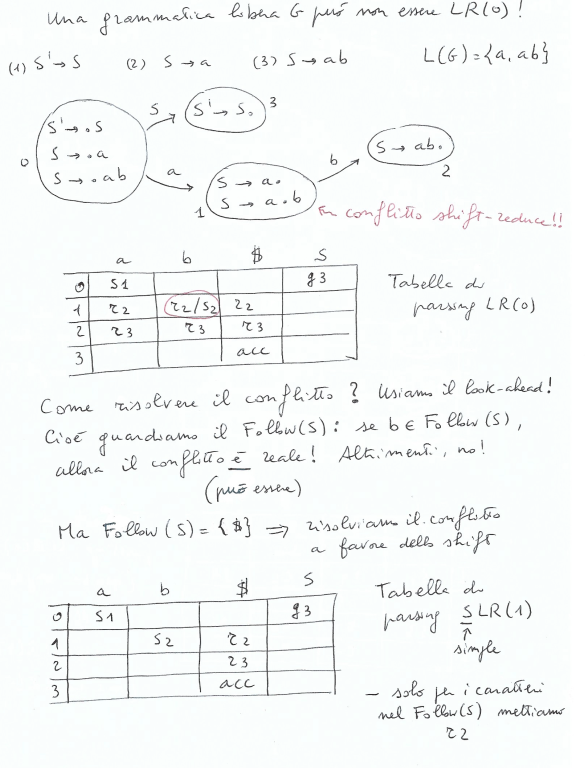
\includegraphics[width=10cm]{esempio-lr-1.png}
}

Ed ecco che entrano in gioco i cosidetti \textbf{Parser LR(1)} che sfruttano gli $item LR(1)$
\subsubsection{Item LR(1)}
\dfn{Item LR(1)}{
    Un itwm $LR(1)$ è una coppia formata da:
    \begin{itemize}
        \item un item LR(0) che viene chiamato nucleo
        \item un simbolo di look-ahead in $T\cup\{\$\}$
    \end{itemize}
}
introdurre questo simbolo di look-ahead è fondamentale, così che si può decidere che azione fare in base al simbolo letto in input 
\esempio{
    Un possibile item $LR(1)$ è:
    \[
        [S\to V.= E, \$]   
    \]
    Dove abbiamo che $S\to V. = E$ è il cuore e $\$$ è il simbolo di look ahead. Se avessi uno stato con due item dentro:
    %! ERRORE GRAFICO, CHE CAZZ È? 
    \[
        \begin{array}{l}
            \lbrack S \to V \cdot E, \, \$\rbrack \\
            \lbrack S \to V \cdot, \, \$\rbrack
        \end{array}
    \]
    In questo caso se leggo il simbolo "=" si avrà uno shift per poi andare in un altro stato grazie al primo item, mentre se si legge $\$$ input avremo un reduce $E\to V$ proprio grazie al simbolo $\$$ di look-ahead
}

\paragraph{Intuizione}: se l'automa canonico $LR(1)$ è in uno stato che contiene l'item $LR(1)\quad [A\to\alpha.\beta,x]$:

\begin{itemize}
    \item $[A\to\alpha.\beta,x]$:
    \begin{itemize}
        \item Sta cercando di riconoscere la maniglia $\alpha \beta$
        \item di essa, $\alpha$ è già sulla pila
        \item Sull'input si aspetta una stringa derivabile da $\beta x$, ovvero si aspetta in input $\beta$ (per fare uno shift) ed un $x$ per la reduce
    \end{itemize}
    \item $[A\to\alpha.,x]$: fai la reduce $A\to \alpha$ se il prossimo input è proprio $x$
\end{itemize}
\subsubsection{NFA LR(1)}

Per creare gli NFA LR(1) si procede in maniera molto simile per NFA LR(0), ma tenendo traccia anche del simbolo di look ahead
\begin{itemize}
    \item Stati: sono item $LR(1)$ della grammatica aumentata
    \item $[S'\to.S, \$]$ è lo stato iniziale
    \item dallo stato $[ato\alpha.X\beta,a]$ c'è una transizione allo stato $[A\to \alpha X.\beta,a]$ etichettata $X$ per $X\in T\cup NT$
    \item dallo stato $[ato\alpha.X\beta,a]$ per $X\in T\cup NT$ e $\forall X\to\gamma$, c'è una $\epsilon$-transizione verso lo stato $\forall b\in First(\beta a).[X\to .\gamma, b]$, dove $First(\beta a)\subseteq T\cup\{\$\}$
\end{itemize}

\subsubsection{Adesso si passa ai DFA LR(0)}

Introduciamo le due funzioni ausiliarie: \textbf{Clos(I) e Goto(I,X)}

\begin{algorithm}
    \caption{Clos}
    \KwIn{I}
    \KwOut{I}

    \While{$I$ non è più modificato}{
        \ForEach{item $[A\to\alpha.X\beta]\in I$}{
            \ForEach{produzione $X\to \gamma$}{
                \ForEach{$b\in First(\beta a)$}{
                    aggiungi $[X\to .\gamma, b]$ ad $I$\;
                }
            }
        }
    }
    \Return $I$\;
\end{algorithm}

\begin{algorithm}
    \caption{Goto}
    \KwIn{I}
    \KwOut{I}

    Inizializza $J=\emptyset$\;
    \ForEach{item $[A\to\alpha.X\beta,a]\in I$}{
        aggiungi $[A\to \alpha X.\beta, a]$ a $J$\;
    }
    \Return $clos(J)$\;
\end{algorithm}
%! altro errore grafico. EH?

Viene presentato, qui, un esempio del grosso automa $LR(1)$
\esempio{
    Sia $G$ la seguente grammatica
    \[
        G = \begin{array}{l}
            0) S'\to S\\
            1) S\to CC\\
            2) C\to cC\\
            3) C\to d
        \end{array}
    \]

    Allora l'automa canonico LR(1) è:
    \begin{center}
    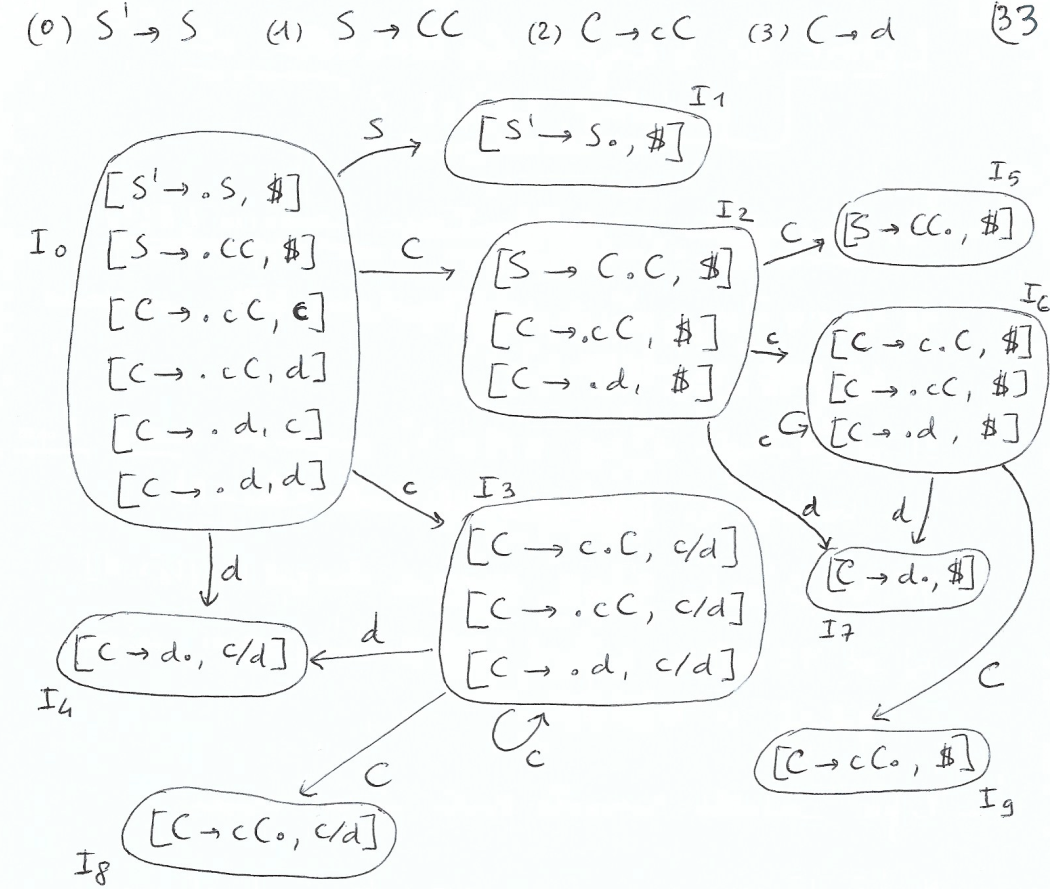
\includegraphics[width=10cm]{giga-automa.png}
    \end{center}
}

\subsubsection{Tabella di parsing $LR(0)$}
Uguale a quella $LR(0)$ e $SLR(1)$ solo che inserisco la reduce solo per il simbolo di look ahead. Riporto comunque la \textit{minghia} di descrizione riportata dal buon Babbo Natale

\begin{enumerate}
    \item Se \( x \in T \) e \( s \xrightarrow{x} t \) nell'automa LR(1), inserisco shift \( t \) in \( M[s, x] \).
    \item Se \([A \to \alpha \cdot, x] \in s\) e \( A 3\neq S' \), inserisco reduce \( A \to \alpha \) in \( M[s, x] \) \textit{(solo per \( x \) del look-ahead!)}.
    \item Se \([S' \to S \cdot, \$] \in s\), inserisco Accept in \( M[s, \$] \).
    \item Se \( A \in NT \) e \( s \xrightarrow{A} t \) nell'automa LR(1), inserisco goto \( t \) in \( M[s, A] \).
\end{enumerate}
\dfn{Grammatica di classe $LR(1)$}{
    Una grammatica libera $G$ e di classe $LR(1)$ se ogni casella della sua tabella di parsing $LR(1)$ contiene al massimo una azione
}

\esempio{
    Si consideri l'automa dell'esempio precedente, allora si ha:

    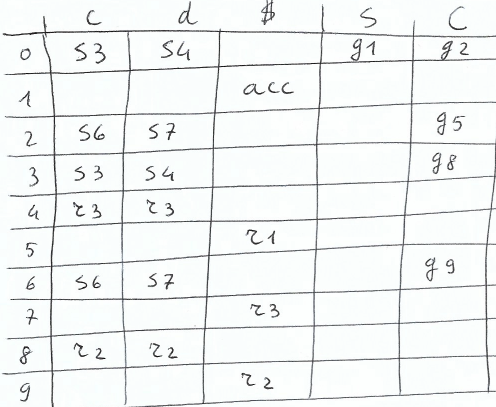
\includegraphics[width=10cm]{parsing-lr-0.png}

    si noti che per questa grammatica la tabella di parsing ha 7 stati anzichè 10, ed è pure senza conflitti 
}

\subsection{Parser $LALR(1)$}

Il problema coi parser $LR(1)$ è che le tabelle sue tabelle di parsing sono molto grandi (centinaia di migliaia di stati per linguaggi di media grandezza), pertanto entrano in gioco i $LALR(1)$ che rappresentano un buon compromesso tra semplicità e selettività

\subsubsection{Come si ottiene il parser $LALR(1)$}


Si osservi che:
\begin{enumerate}
    \item \textbf{Nucleo di uno stato LR(1)}: \\
    L'insieme di item LR(0) ottenuto dimenticando i \textit{look-ahead} dagli item LR(1).
    
    \item \textbf{Nucleo di stato LR(1)}: \\
    Ogni nucleo di uno stato LR(1) corrisponde a uno stato dell'automa LR(0).
    
    \item \textbf{Transizioni dell'automa LR(1)}: \\
    Le transizioni dell'automa LR(1) dipendono solo dal nucleo. La funzione \( \text{goto}(I, X) \) usa di \( I \) solo le parti ``nucleo/LR(0)'' degli item LR(1).
\end{enumerate}

\subsubsection{Tabella di parsing LALR(1)}
La tabella di parsing LALR(1) si ottiene da quella LR(1) \textbf{fondendo insieme gli stati con lo stesso nucleo}. \\
Ciò comporta:
\begin{itemize}
    \item \textbf{Meno righe}, poiché gli stati dell'automa LR(0) vengono combinati.
    \item \textbf{Meno reduce} rispetto alla tabella SLR(1).
\end{itemize}

\esempio{
    Sia la grammatica degli esempi precedenti, ecco qui il nostro automa
    \begin{center}
    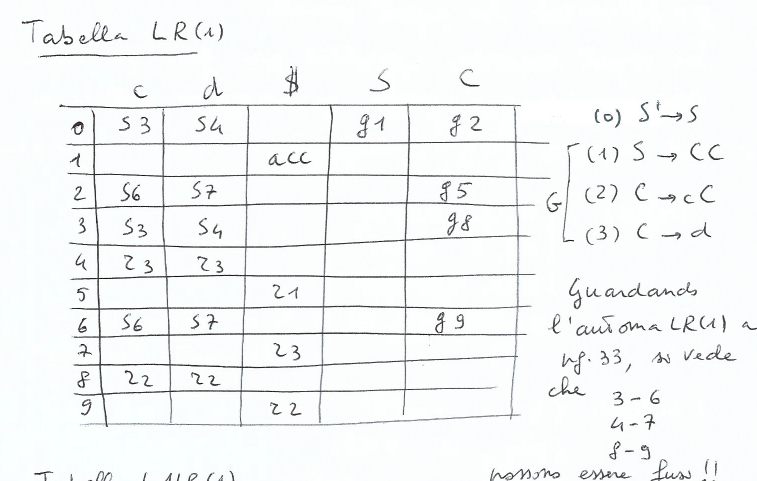
\includegraphics[width=10cm]{parsing-lalr-1.png}
    \end{center}
}

\subsubsection{Passando da lr(1) a LALR(1)}

La fusione di due stati $LR(1)$ con lo stesso core può causare conflitti

\thm{Babbo natale Theorem}{
    Quando fondo due stati $LR(1)$ per generare un parser $LALR(1)$ sono possibili solo conflitti \textbf{reduce/reduce}
}
\dimostrazione{
    Supponiamo che in $s$, stato ottenuto dalla fusione di due stati $LR(1)$, $s_1$ ed $s_2$

    Allora in $s$ esiste un item $[S\to\alpha.a]$ e un item $[B\to\beta.a\gamma, b]$ (H1)

    Suppongo che $[A\to\alpha.,a]\in s_1$ (H2)

    per (H1) $[A\to\alpha., a]\in s_1$ e $[B\to\beta.a\gamma,c]\in s_1$ (H3) dato che se ho fuso insieme $s_1$ ed $s_2$ allora il core $[B\to\beta.a\gamma]$ deve per forza esserci in entrambi $\heartsuit$

    Per (H3) si ha che anche in $LR(1)$ si verificherebbe un conflitto shift-reduce, contro l'ipotesi che la tabella $lr(1)$ non presenti conflitti, pertanto se $LR(1)$ è senza conflitti, $LARL(1)$ potrebbe solo presentare conflitti reduce-reduce
}

\nt{
    Se si generano conflitti, allora $G$ non è $LALR(1)$, pur essendo $LR(1)$
}

\esempio{
    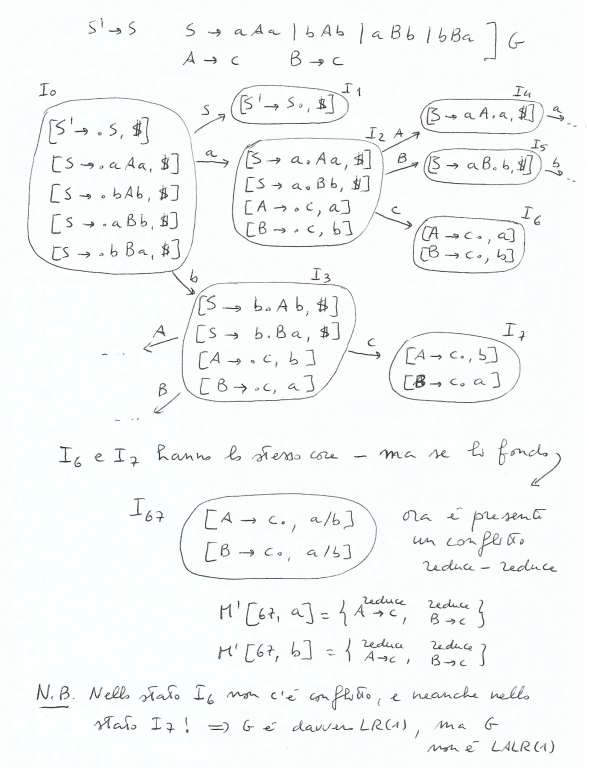
\includegraphics[width=10cm]{ultimo-lalr-1.png}
}

\section{Grammatiche $LR(k)$}
Ci si può concentrare adesso alle grammatiche $LR$ con $k$ simboli di look-ahead, nessuno le usa perché molto confusionarie e macchinose, ma si possono andare a definire

Prima della definizione di grammatica occorre definire \textbf{gli item $LR(k)$}

\dfn{
    Item $LR(k)$
}{
    Si definisce un \textbf{item $LR(k)$}, un item formato da una coppia formata da un item $LR(0)$ e una stringa $\beta$ la cui lunghezza è inferiore a $k$, e si denota nel seguente modo:
    \[
        [item\;LR(0), \beta] \text{ con }|\beta|\leq k
    \]
}

Tali item hanno queste caratteristiche:
\begin{itemize}
    \item Lo stato iniziale è sempre $[S'\to.S, \$]$
    \item Sia $s$ uno stato dell'automa canonico $LR(k)$, si che $([A\to \alpha.X\gamma, \beta]\in s\land \exists \text{ la produzione }X\to \gamma\land w\in First_k(\gamma\beta ) ) \implies [X\to.\gamma ,w]\in s$ 
\end{itemize}

Si può subito intuire che un automa canonico $LR(k)$ genera una quantità molto grande di stati molto difficili da gestire a mano

Una volta costruito l'automa canonico $LR(k)$ si passa alla tabella di parsing $LR(k)$ con collonne su $T^k$ (cioè su stringhe di terminali lunghe $k$)

\dfn{Grammatica $LR(k)$}{
    Si definisce $G$ una grammatica $LR(k)$ una grammatica costruita a partire da una tabella di parsing $LR(k)$, ottenuta a partire dall'automa canonico $LR(k)$, con le seguenti caratteristiche:
    \begin{itemize}
        \item Contiene al più un'azioni per ogni entrata della tabella
        \item non esistono sue $w_1$ e $w_2$ sulle colonne tali che $w_1$ è prefisso di $w_2$ e per almeno una righe le 2 corrispondenti entrate contengono un'azione
    \end{itemize}
}

\nt{Ovviamente la tabella viene tiempita nel modo ovvio per le azioni di shift/accept, mentre le reduce sono messe solo in corrispondenza del lookahead, ad esempio $[A\to\alpha.,w]$}

\subsection{Grammatiche $SLR(k)$}

Si parte dell'automa canonico $LR(0)$ e si riempie la tabella di parsing $SLR(k)$ - che ha colonne su $T^k$ - secondo la seguente legge: 
\[
    ([A\to\alpha.]\in s\land A\neq S')\implies \forall w\in Follow_k(A).(M[s,w]=\text{ reduce } A\to\alpha)
\] 

\subsection{
    Grammatiche $LALR(k)$
}
Si parte dall'automa canonico $LR(k)$ e si fondono insieme due stato con lo stesso nucleo, se non vi sono conflitti $G$ è $LALR(k)$

\subsection{relazione tra le varie grammatiche}
Si può noti il seguente schema riassuntivo:
\begin{center}
    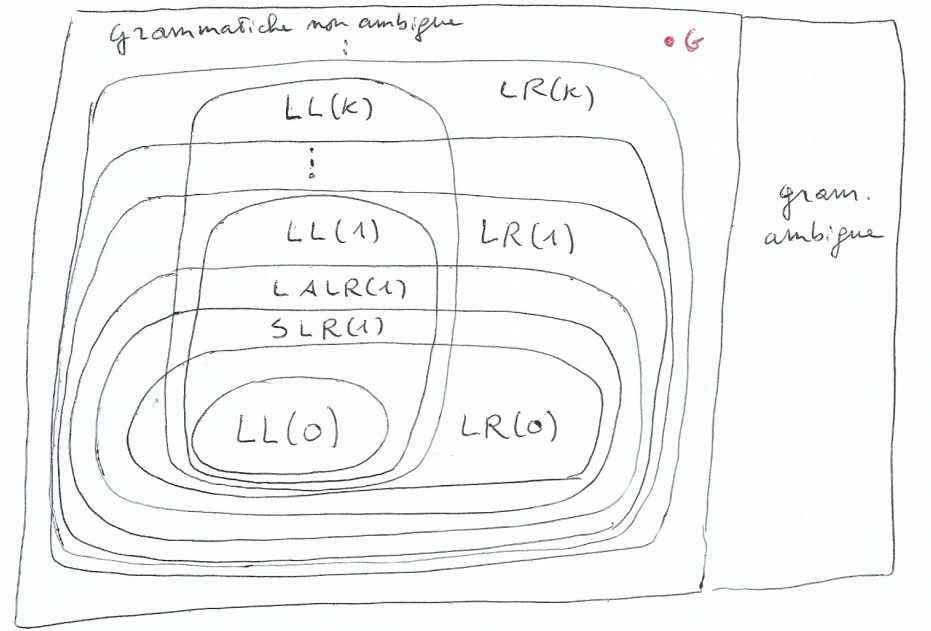
\includegraphics[width=10cm]{inclusione-tra-grammatiche.png}
\end{center}

Si può concludere che:
\[
LR:
\begin{cases}
    \text{SLR}(k) \subset \text{LALR}(k) \subset \text{LR}(k) & \text{per ogni } k \geq 1 \\
    \text{SLR}(1) \subset \text{SLR}(2) \subset \dots \subset \text{SLR}(k) \\
    \text{LALR}(1) \subset \text{LALR}(2) \subset \dots \subset \text{LALR}(k) \\
    \text{LR}(0) \subset \text{LR}(1) \subset \dots \subset \text{LR}(k)
\end{cases}
\]

\textbf{LL vs LR:}
\[
LL vs LR:
\begin{cases}
    \text{LL}(k) \subset \text{LR}(k) & \text{per ogni } k \geq 0 \\
    \text{LL}(k) \not\subset \text{LR}(k-1) & \text{per ogni } k \geq 1
\end{cases}
\]

\mprop{}{
    \begin{itemize}
        \item Se $G$ è $LL(k)$, allora $G$ è non ambigua e $L(G)$ è deterministico
        \item Se $G$ è $LR(k)$, allora $G$ è non ambigua e $L(G)$ è deterministico
    \end{itemize}
}
\nt{
    Esistono linguaggi generati da grammatiche non ambigue, ma nondeterministici
}

\esempio{
    Sia $G$ la seguente grammatica:
    \[
        S\to aSa\mid bSb\mid\epsilon      
    \]
    Allora
    \[
        L(G) = \{ww^R\mid w\in\{a,b\}^*\}
    \]
}

\section{Linguaggi generati dalle varie grammatiche}
\dfn{
    Linguaggio di classe $X$
}{
    Un linguaggio $L$ si definisce di classe $X$ se $\exists G$ di classe $X$ tale che $L=L(G)$

    Dove $X$ sta per $LR(0)/SLR(1)/LL(1)/\dots$
}
Se classifichiamo i linguaggi anziché le grammatica, il diagramma si semplifica molto

\esempio{
    \begin{center}
    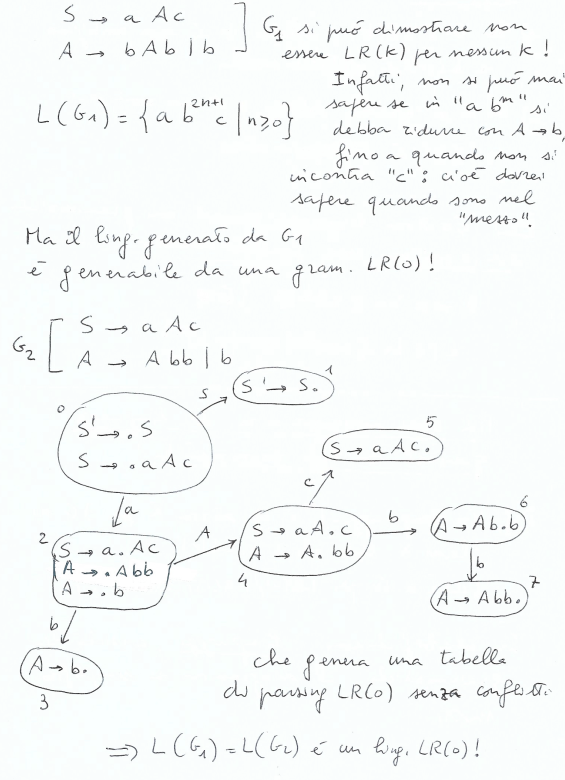
\includegraphics[width=10cm]{esempio-linguaggio.png}
    \end{center}
}
Si considerino queste note

\nt{
    Un linguaggio è libero deterministico se è accettato, per stato dinale 
}
\nt{
    Ogni linguaggio regolare è generato da una grammatica di classe $LL(1)$
}
\nt{
    esistono linguaggi regolari che non sono $LR(0)$ 

    Ad es. $L=\{a,ab\}$
}
Si considerino i seguenti teoremi:
\teorema{
    Un linguaggio è libero deterministico sse è generato da una grammatica $LR(1)$ per qualche $k\geq 0$
}
\teorema{
    Un linguaggio è libero deterministico sse è generato da una grammatica $SLR(1)$
}
\teorema{
    I linguaggi generati da grammatica $LL(k)$ sono esattamente contenuti nei linguaggi generati da grammatiche $SLR(1),\forall k\geq 0$
}
\subsubsection{calssificazione dei linguaggi}
Si noti il seguente schema:
\begin{center}
    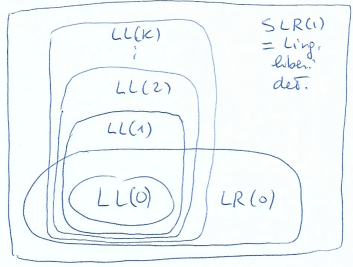
\includegraphics[width=10cm]{classificazione-dei-linguaggi.png}
\end{center}
\nt{
    Se $G$ è $LR(k)$, esiste $G'\in SLR(1)$ quivalente, ma $G'$ può essere molto più complessa di $G$ 
}

\esempio{
    Sia $L=\{a^i b^j\mid i\geq j\geq 0\}$ libero deterministico

    Si può notare che
    \begin{center}
        \begin{tikzpicture}
            \node[state, initial] (q) {$q_0$};
            \node[state, right of=q] (q1) {$q_1$};
            
            \path[->] 
                    (q_0) edge [loop above] node {$a, X/aX$} ()
                        edge  node {$b,a/\epsilon$} (q1)
                    (q_1) edge [loop above]  node {$b,a/\epsilon$} ();
        \end{tikzpicture}  
    \end{center}
    è il DPDA che riconosce $L$ per stato finale

    $L$ però non è $LL(k)$ per nessun $k$, tuttavia $L$ è $SLR(1)$, infatti esiste $G$ $SLR(1)$ tale che $L(G)=L$:
    \[
        \begin{array}{l}
            S\to aS\mid B\\
            B\to aBb\mid \epsilon
        \end{array}
    \]
    \begin{center}
    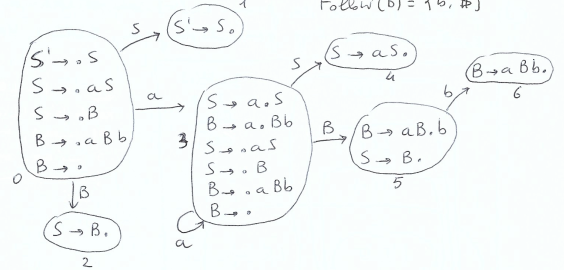
\includegraphics[width=10cm]{automa-bellino.png}
    \end{center}

    La cui tabella di parsing è:
    \[
        \begin{array}{c|c|c|c|c|c}
        & a & b & \$ & S & B \\
        \hline
        0 & S_3 & R_4 & R_4 & G_1 & G_2 \\
        1 & & & \text{acc} & & \\
        2 & & & R_2 & & \\
        3 & S_3 & R_4 & & G_4 & G_5 \\
        4 & & & R_4 & & \\
        5 & S_3 & & R_2 & & \\
        6 & R_3 & R_3 & & &
        \end{array}
    \]

    \textit{Tabella di parsing SLR(1) senza conflitti} \\
    $\Rightarrow G$ è SLR(1)
}

\nt{
    \begin{enumerate}
        \item $L_1 = \{ a^n b^n \mid n \geq 1 \} \in \text{LL}(1) \in \text{LR}(0)$ \\
            $L_2 = \{ a^n c^m \mid n, m \geq 1 \} \in \text{LL}(1) \in \text{LR}(0)$ \\
            
            ma $L_1 \cup L_2$ non è $\text{LL}(k)$ per nessun $k$, \\
            mentre $L_1 \cup L_2 \in \text{LR}(0)$ \\
            $\Rightarrow$ l'unione di linguaggi $\text{LL}(1)$ può non essere $\text{LL}(1)$
        \item $L_1 = \{ a \} \in \text{LL}(1) \in \text{LR}(0)$ \\
            $L_2 = \{ a b \} \in \text{LL}(1) \in \text{LR}(0)$ \\
            
            ma $L_1 \cup L_2$ non è $\text{LR}(0)$ perché non gode della prefix-property, \\
            mentre $L_1 \cup L_2 \in \text{LL}(1)$ \\
            $\Rightarrow$ l'unione di linguaggi $\text{LR}(0)$ può non essere $\text{LR}(0)$
        \item $L_1 = a^* = \{ a^n \mid n \geq 0 \} \in \text{LL}(1)$ \\
            $L_2 = \{ a^n b^n \mid n \geq 0 \} \in \text{LL}(1)$ \\
            
            ma $L_1 \cdot L_2 = \{ a^i b^j \mid i \geq j \geq 0 \}$ non è $\text{LL}(k)$ per nessun $k$ \\
            $\Rightarrow$ la concatenazione di due linguaggi $\text{LL}(1)$ può non essere $\text{LL}(1)$
    \end{enumerate}
}


zio pera
\end{document}